\documentclass[12pt,]{article}
%\usepackage{lmodern}  Melissa removed to deal with font rendering issue
\usepackage{amssymb,amsmath}
\usepackage{ifxetex,ifluatex}
\usepackage{fixltx2e} % provides \textsubscript

%Melissa removed the following section to deal with font rendering issue
%\ifnum 0\ifxetex 1\fi\ifluatex 1\fi=0 % if pdftex
%  \usepackage[T1]{fontenc}
%  \usepackage[utf8]{inputenc}
%%\else % if luatex or xelatex
%  \ifxetex
%    \usepackage{mathspec}
%  \else
%    \usepackage{fontspec}
%  \fi
%  \defaultfontfeatures{Ligatures=TeX,Scale=MatchLowercase}
%  \newcommand{\euro}{€}
%%%%%%\fi

% use upquote if available, for straight quotes in verbatim environments
\IfFileExists{upquote.sty}{\usepackage{upquote}}{}
% use microtype if available
\IfFileExists{microtype.sty}{%
\usepackage{microtype}
\UseMicrotypeSet[protrusion]{basicmath} % disable protrusion for tt fonts
}{}
\usepackage[margin=1in]{geometry}
\usepackage{hyperref}
\PassOptionsToPackage{usenames,dvipsnames}{color} % color is loaded by hyperref
\hypersetup{unicode=true,
            pdftitle={The Combined Status of Gopher (Sebastes carnatus) and Black-and-Yellow Rockfishes (Sebastes chrysomelas) in U.S. Waters Off California in 2019},
            pdfborder={0 0 0},
            breaklinks=true}
\urlstyle{same}  % don't use monospace font for urls
\usepackage{graphicx,grffile}
\makeatletter
\def\maxwidth{\ifdim\Gin@nat@width>\linewidth\linewidth\else\Gin@nat@width\fi}
\def\maxheight{\ifdim\Gin@nat@height>\textheight\textheight\else\Gin@nat@height\fi}
\makeatother
% Scale images if necessary, so that they will not overflow the page
% margins by default, and it is still possible to overwrite the defaults
% using explicit options in \includegraphics[width, height, ...]{}
\setkeys{Gin}{width=\maxwidth,height=\maxheight,keepaspectratio}
\setlength{\parindent}{0pt}
\setlength{\parskip}{6pt plus 2pt minus 1pt}
\setlength{\emergencystretch}{3em}  % prevent overfull lines
\providecommand{\tightlist}{%
  \setlength{\itemsep}{0pt}\setlength{\parskip}{0pt}}
\setcounter{secnumdepth}{5}

%%% Use protect on footnotes to avoid problems with footnotes in titles
\let\rmarkdownfootnote\footnote%
\def\footnote{\protect\rmarkdownfootnote}

%%% Change title format to be more compact
\usepackage{titling}

% Create subtitle command for use in maketitle
\newcommand{\subtitle}[1]{
  \posttitle{
    \begin{center}\large#1\end{center}
    }
}

\setlength{\droptitle}{-2em}
  \title{The Combined Status of Gopher (\emph{Sebastes carnatus}) and
Black-and-Yellow Rockfishes (\emph{Sebastes chrysomelas}) in U.S. Waters
Off California in 2019}
  \pretitle{\vspace{\droptitle}\centering\huge}
  \posttitle{\par}
  \author{}
  \preauthor{}\postauthor{}
  \date{}
  \predate{}\postdate{}


% This file contains all of the LaTeX packages you may need to compile the document
% Documentation for each package can be found onlines
\usepackage{tabularx}                                             % table environment providing flexibility
\usepackage{caption}                                              % for creating captions  
\usepackage{longtable}                                            % allows tables to span multiple pages
\usepackage{rotating}                                             % allows for sideways tables
\usepackage{float}                                                % floating environments; may not need in rmarkdown
\usepackage{placeins}                                             % keeps floats from moving
\usepackage{indentfirst}                                          % indents first paragraph of a section
\usepackage{mdwtab}                                               % continued float multi-page figure
\usepackage{enumerate}                                            % create lists
\usepackage{hyperref}                                             % highlight cross references
\hypersetup{colorlinks=true, urlcolor=blue, linktoc=page, linkcolor=blue, citecolor=blue} %define referencing colors
%\usepackage{makebox}                                             % make boxes around text
\usepackage[usenames,dvipsnames]{xcolor}                          % color name options
%\usepackage[space]{grffile}                                      % spaces in file name path
\usepackage{soul}                                                 % highlight text
\usepackage{enumitem}                                             % numbered lists
\usepackage{lineno}                                               % Line numbers; comment out for final
\usepackage{upquote}                                              % produce grave accent in latex
\usepackage{verbatim}                                             % produces verbatim results
\usepackage{fancyvrb}                                             % verbatim in a box
\usepackage{textcomp}                                             % fixes error with packages interfering
\usepackage{lscape}                                               % rotate pages - to allow for landscape longtables
%\pdfinterwordspaceon                                             % fix loss of inter word spacing
\usepackage{cmap}                                                 % fix mapping characters to unicode
\RequirePackage[linewidth = 1]{pdfcomment}                        % pdf comments
\RequirePackage[l2tabu, orthodox]{nag}                            % checks packages related to the accessibility?
%\usepackage[inline]{showlabels}                                   % show table and figure labels; comment                                                                      out for final
%\RequirePackage[tagged]{accessibilityMeta}
\usepackage{booktabs} 

%\linenumbers                                                      % specify use of line numbers


\definecolor{light-gray}{gray}{.85}                               % define light-gray as a color
%\usepackage[tagged]{accessibility-meta}

 
%\showlabels[\color{mred}]{label}

% Redefines (sub)paragraphs to behave more like sections
\ifx\paragraph\undefined\else
\let\oldparagraph\paragraph
\renewcommand{\paragraph}[1]{\oldparagraph{#1}\mbox{}}
\fi
\ifx\subparagraph\undefined\else
\let\oldsubparagraph\subparagraph
\renewcommand{\subparagraph}[1]{\oldsubparagraph{#1}\mbox{}}
\fi

\begin{document}
\maketitle


\begin{center}
\thispagestyle{empty}


\vspace{.5cm}

%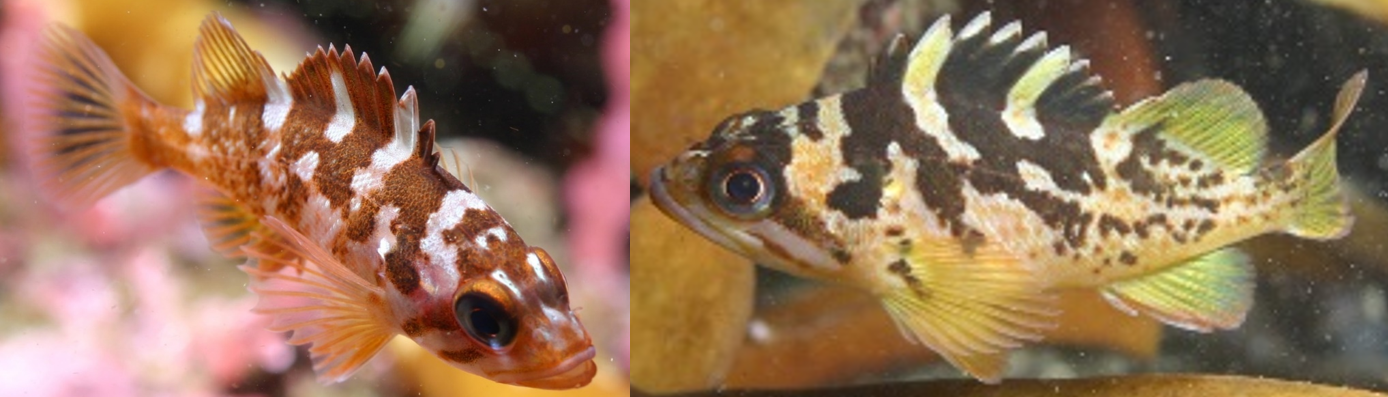
\includegraphics{cover_photo}~\\[1cm]
\pdftooltip{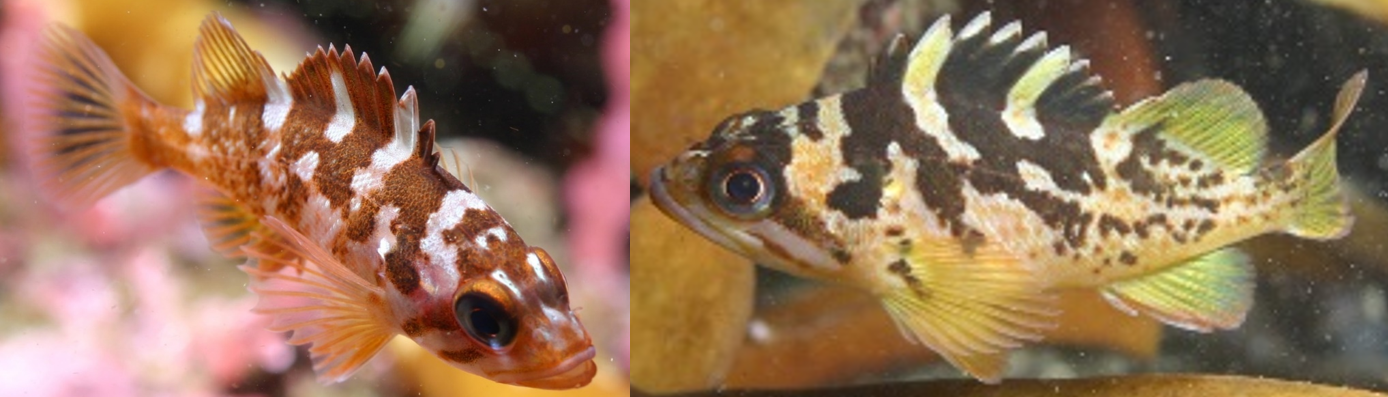
\includegraphics{cover_photo}}{This is a fish.}
Gopher rockfish (left) and black-and-yellow rockfish (right).      
\small
Photos by Steve Lonhart.

\vspace{.3cm}


Melissa H. Monk\textsuperscript{1}\\
Xi He\textsuperscript{1}\\

\vspace{.5cm}

\small
\textsuperscript{1}Southwest Fisheries Science Center, U.S. Department of Commerce, National Oceanic and Atmospheric Administration, National Marine Fisheries Service, 110 McAllister Way, Santa Cruz, California 95060\\

\vspace{1.5cm}


%\vfill
%DRAFT SAFE\\
Disclaimer: This information is distributed solely for the purpose of pre-dissemination
peer review under applicable information quality guidelines. It has not been formally
disseminated by NOAA Fisheries. It does not represent and should not be construed to
represent any agency determination or policy. 

\vspace{.1cm}
%Bottom of the page
%{\large \today}


\newpage{\thispagestyle{empty}}


\begin{flushleft}
This report may be cited as:

Monk, M. H.  and X. He. 2019. The Combined Status of Gopher \emph{Sebastes carnatus} and Black-and-Yellow Rockfishes \emph{Sebastes chrysomelas} in U.S. Waters Off California in 2019. Pacific Fishery Management Council, Portland, OR. Available from http://www.pcouncil.org/groundfish/stock-assessments/
\end{flushleft}

\maketitle

\pagenumbering{roman}
\setcounter{page}{1}
\end{center}

{
\setcounter{tocdepth}{4}
\tableofcontents
}
\setlength{\parskip}{5mm plus1mm minus1mm} \pagebreak

\setcounter{page}{1} \renewcommand{\thefigure}{\alph{figure}}
\renewcommand{\thetable}{\alph{table}}

\section*{Executive Summary}\label{executive-summary}
\addcontentsline{toc}{section}{Executive Summary}

\subsection*{Stock}\label{stock}
\addcontentsline{toc}{subsection}{Stock}

This assessment reports the status of the gopher and black-and-yellow
rockfish\\
complex (GBYR, \emph{Sebastes carnatus/Sebastes chrysomelas}) resource
in U.S. waters off the coast of California south of Cape Mendocino
(\(40^\circ 10^\prime\) N. latitude) using data through 2018. Both
gopher and black-and-yellow rockfishes are most abundant north of Point
Conception (\(34^\circ 27^\prime\) N. latitude) and are uncommon north
of Point Arena (\(38^\circ 57^\prime\) N. latitude). The range of gopher
rockfish extends into Baja California, but the black-and-yellow rockfish
are rare south of Point Conception.

\subsection*{Catches}\label{catches}
\addcontentsline{toc}{subsection}{Catches}

Information on historical landings of GBYR are available back to 1916
(Table \ref{tab:Exec_catch}). The recreational fleet began ramping up in
the 1950s and has fluctuated over the the last 50 years (Figure
\ref{fig:Exec_catch1}). The majority of GBYR recreational landings have
been from north of Point Conception throughtout the time period
modelled.

Commercial landings were small during the years of World War II, ranging
between 4 to 28 metric tons (mt) per year (Figure
\ref{fig:Exec_catch2}). Commercial landings increased after World War II
and show periods of cyclical catch for gopher and black-and-yellow
rockfishes. The commercial live fish fishery began in the early 1990s,
with the first reported live landings in 1993. Since then the commercial
catch has been dominated by the live fish fishery, with minimal landings
of dead gopher or black-and-yellow rockfishes. Estimates of total
mortality of commercial discards were available starting in 2004, and
were estimated prior to then. The catches aggregated by fleets modeled
in this assessment can be found in Figure \ref{fig:r4ss_catches}.

Since 2000, annual total landings of catch and discards of GBYR have
ranged between 70-169 mt, with landings (catch + discards) in 2018
totaling 92 mt.

\FloatBarrier

\begin{figure}
\centering
\includegraphics{Figures/rec_exec.png}
\caption{Catch history of GBYR landings for the recreational fleet north
(RecNorth) and south (RecSouth) of Point Conception..
\label{fig:Exec_catch1}}
\end{figure}

\begin{figure}
\centering
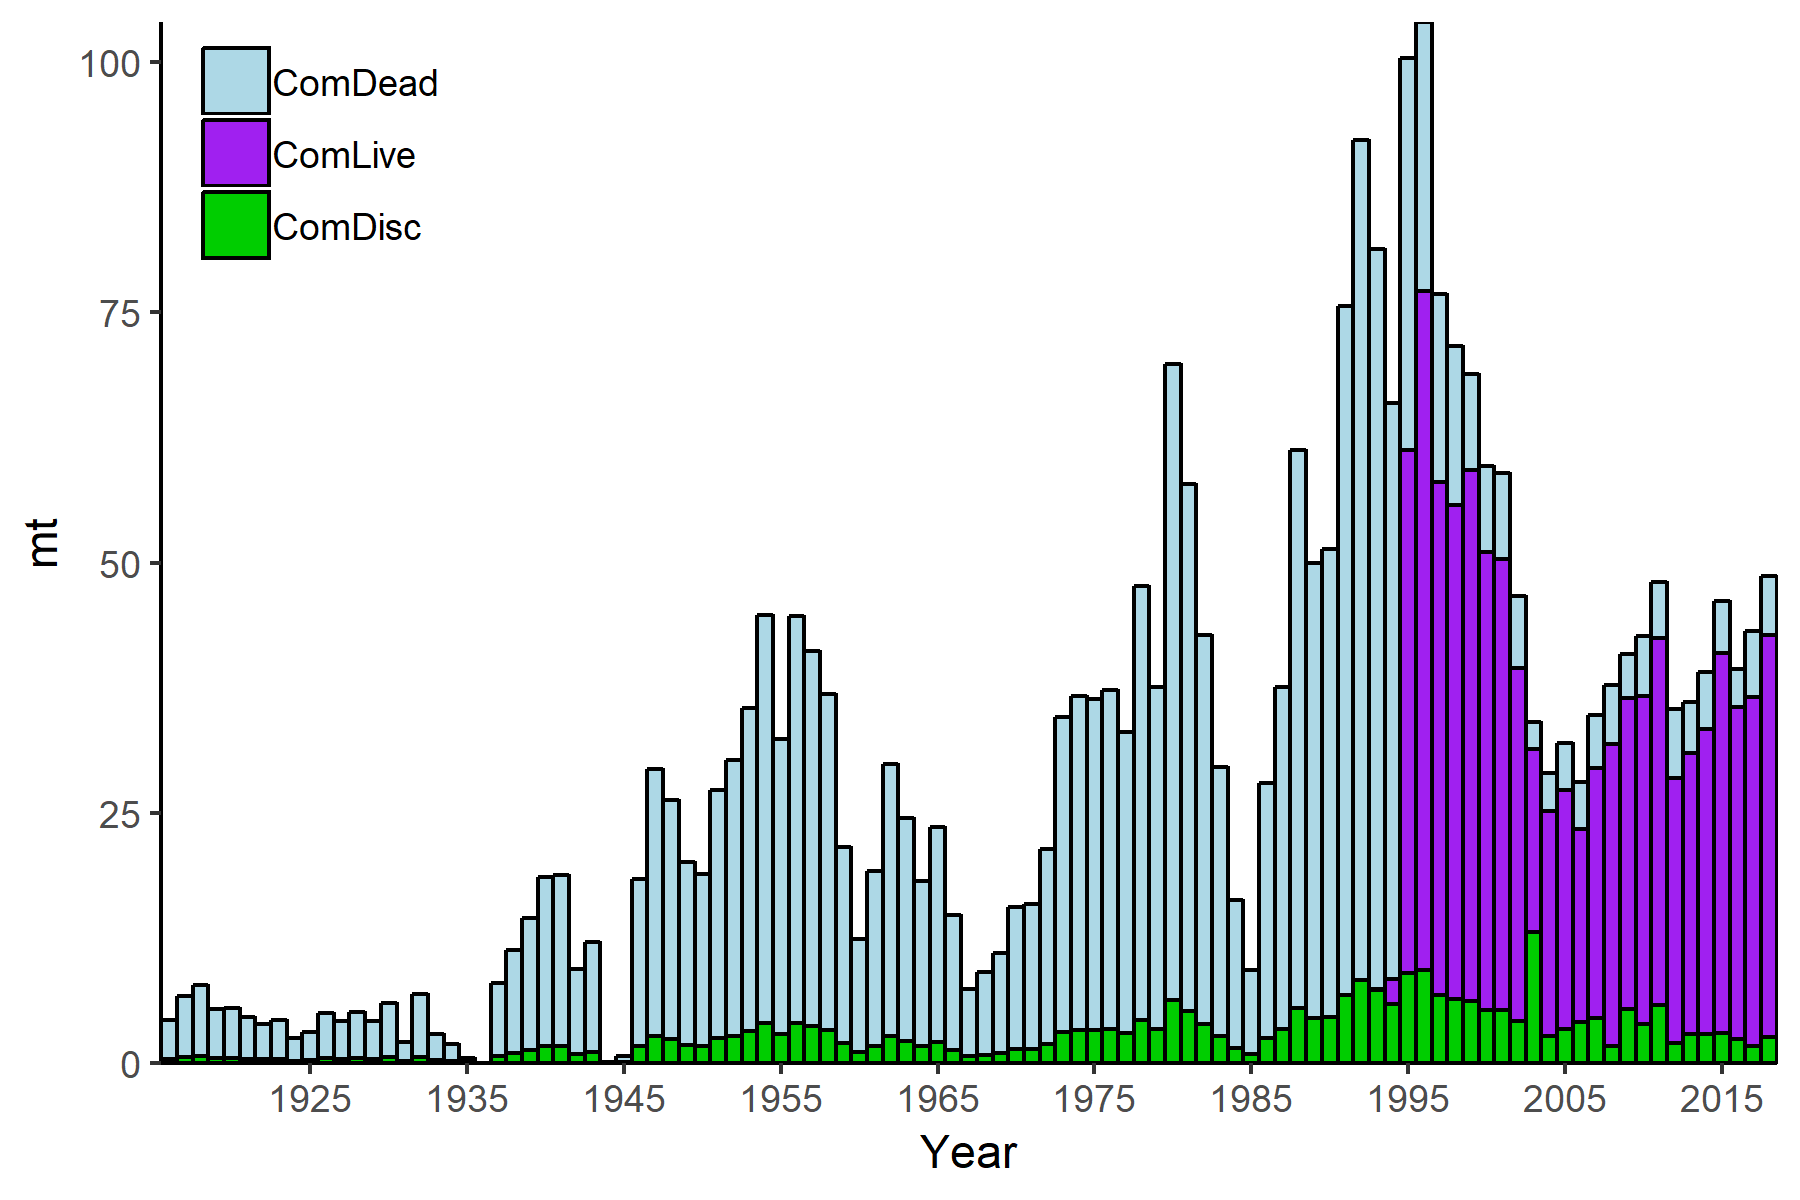
\includegraphics{Figures/comm_exec.png}
\caption{Catch history of GBYR for the commercial fleet by dead
(ComDead) and live (ComLive) landings, and discards (ComdDisc). Catches
in 1936 and 1946 were minimal. \label{fig:Exec_catch2}}
\end{figure}

\FloatBarrier

\begin{figure}
\centering
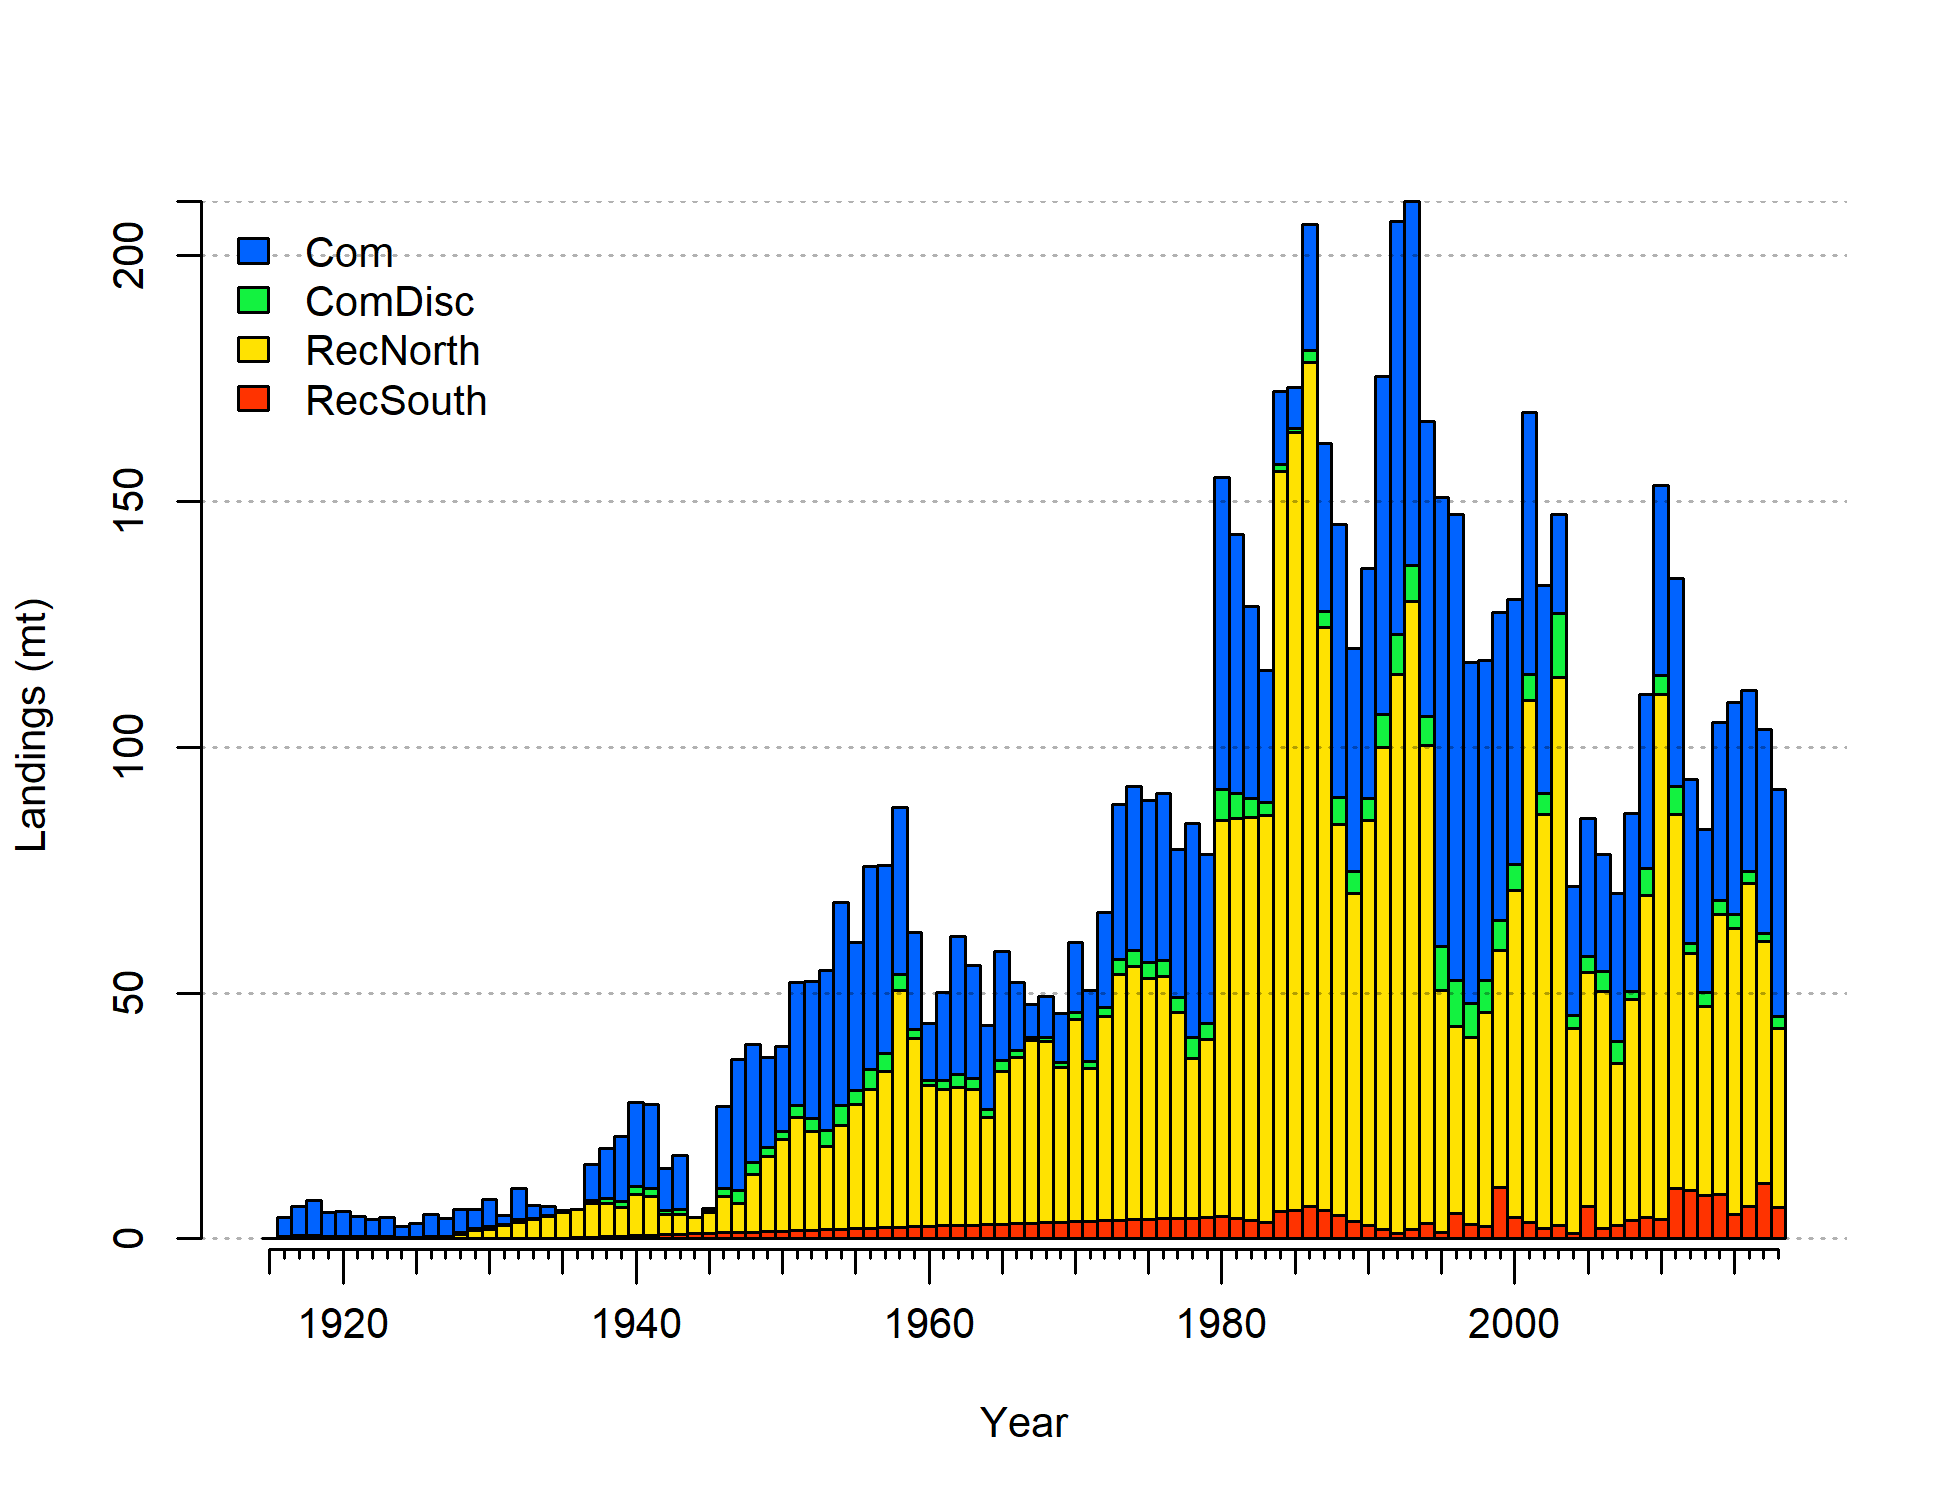
\includegraphics{r4ss/plots_mod1/catch2 landings stacked.png}
\caption{Catch history of GBYR in the model. \label{fig:r4ss_catches}}
\end{figure}

\begin{table}[ht]
\centering
\caption{Recent GBYR landings (mt) by 
                                            fleet, where the recreational fleet 
                                            is split at Point Conception.} 
\label{tab:Exec_catch}
\begin{tabular}{l>{\centering}p{1in}>{\centering}p{1in}>{\centering}p{1in}>{\centering}p{.9in}>{\centering}p{.9in}}
  \hline
Year & Commercial Retained & Commercial Discard & Recreational North & Recreational South & Total \\ 
  \hline
2009 & 35.62 & 5.38 & 65.64 & 4.30 & 110.93 \\ 
  2010 & 38.83 & 3.92 & 106.76 & 3.90 & 153.41 \\ 
  2011 & 42.39 & 5.72 & 76.16 & 10.24 & 134.52 \\ 
  2012 & 33.55 & 1.93 & 48.25 & 9.89 & 93.62 \\ 
  2013 & 33.45 & 2.85 & 38.43 & 8.86 & 83.59 \\ 
  2014 & 36.40 & 2.85 & 56.96 & 9.06 & 105.27 \\ 
  2015 & 43.25 & 2.93 & 58.09 & 5.00 & 109.27 \\ 
  2016 & 36.96 & 2.42 & 65.72 & 6.57 & 111.67 \\ 
  2017 & 42.04 & 1.65 & 49.36 & 11.15 & 104.19 \\ 
  2018 & 47.00 & 2.54 & 36.48 & 6.30 & 92.32 \\ 
   \hline
\end{tabular}
\end{table}

\FloatBarrier

\newpage

\subsection*{Data and Assessment}\label{data-and-assessment}
\addcontentsline{toc}{subsection}{Data and Assessment}

Gopher rockfish north of Point Conception (\(34^\circ 27^\prime\) N.
latitude) was first assessed as a full stock assessment in 2005 (Key et
al. \protect\hyperlink{ref-Key2005}{2005}) using SS2 (version 1.19). The
assessment was sensitive to the recreational party boat onboard observer
index of relative abundance (referred to as Deb Wilson-Vandenberg's
onboard observer index in this assessment). The final decision table was
based around the emphasis given to this index of relative abundance. The
stock was found to be at 97\% depletion in 2005.

Gopher rockfish south of Point Conception was assessed as a data poor
species in 2010 (Dick and MacCall
\protect\hyperlink{ref-Dick2010}{2010}). A Depletion-Corrected Average
Catch (DCAC) model was used due to time constraints. The mean yield from
the DCAC distribution was 25.5 mt.

This is the first full assessment to include data for black-and-yellow
rockfish. Black-and-yellow rockfish was assessed coastwide as a data
poor species using Depletion-Based Stock Reduction Analysis (DB-SRA)
(Dick and MacCall \protect\hyperlink{ref-Dick2010}{2010}). The DB-SRA
model assigned a 40\% probability that the then recent (2008-2009) catch
exceeded the 2010 OFL.

This assessment of the GBYR complex covers the area from Cape Mendocino
to the U.S./Mexico border (Figure \ref{fig:assess_region_map}). The
length composition data suggested that while the lengths of gopher and
black-and-yellow rockfish were similar, fish encountered south of Point
Conception were smaller. The similarity of the length distributions
between species and among modes within a region were similar and
justified one combined recreational fleet within each of the two regions
(north and south of Point Conception).

This stock assessment retains a single fleet for the commercial fishery,
including discards. Data on commercial discards were not available for
and not included in the 2005 assessment. The decision to retain one
commercial fleet was made by examining the length distributions across
species, fishing gears, and space, i.e., north and south of Point
Conception. There is very little difference between the length
composition of gopher and black-and-yellow rockfish landed in the
commercial fleet north and south of Point Conception.

A number of sources of uncertainty are addressed in this assessment.
This assessment includes length data, estimated growth, an updated
length-weight curve, an updated maturity curve, a number of new indices,
and new conditional age-at-length data.

\begin{figure}
\centering
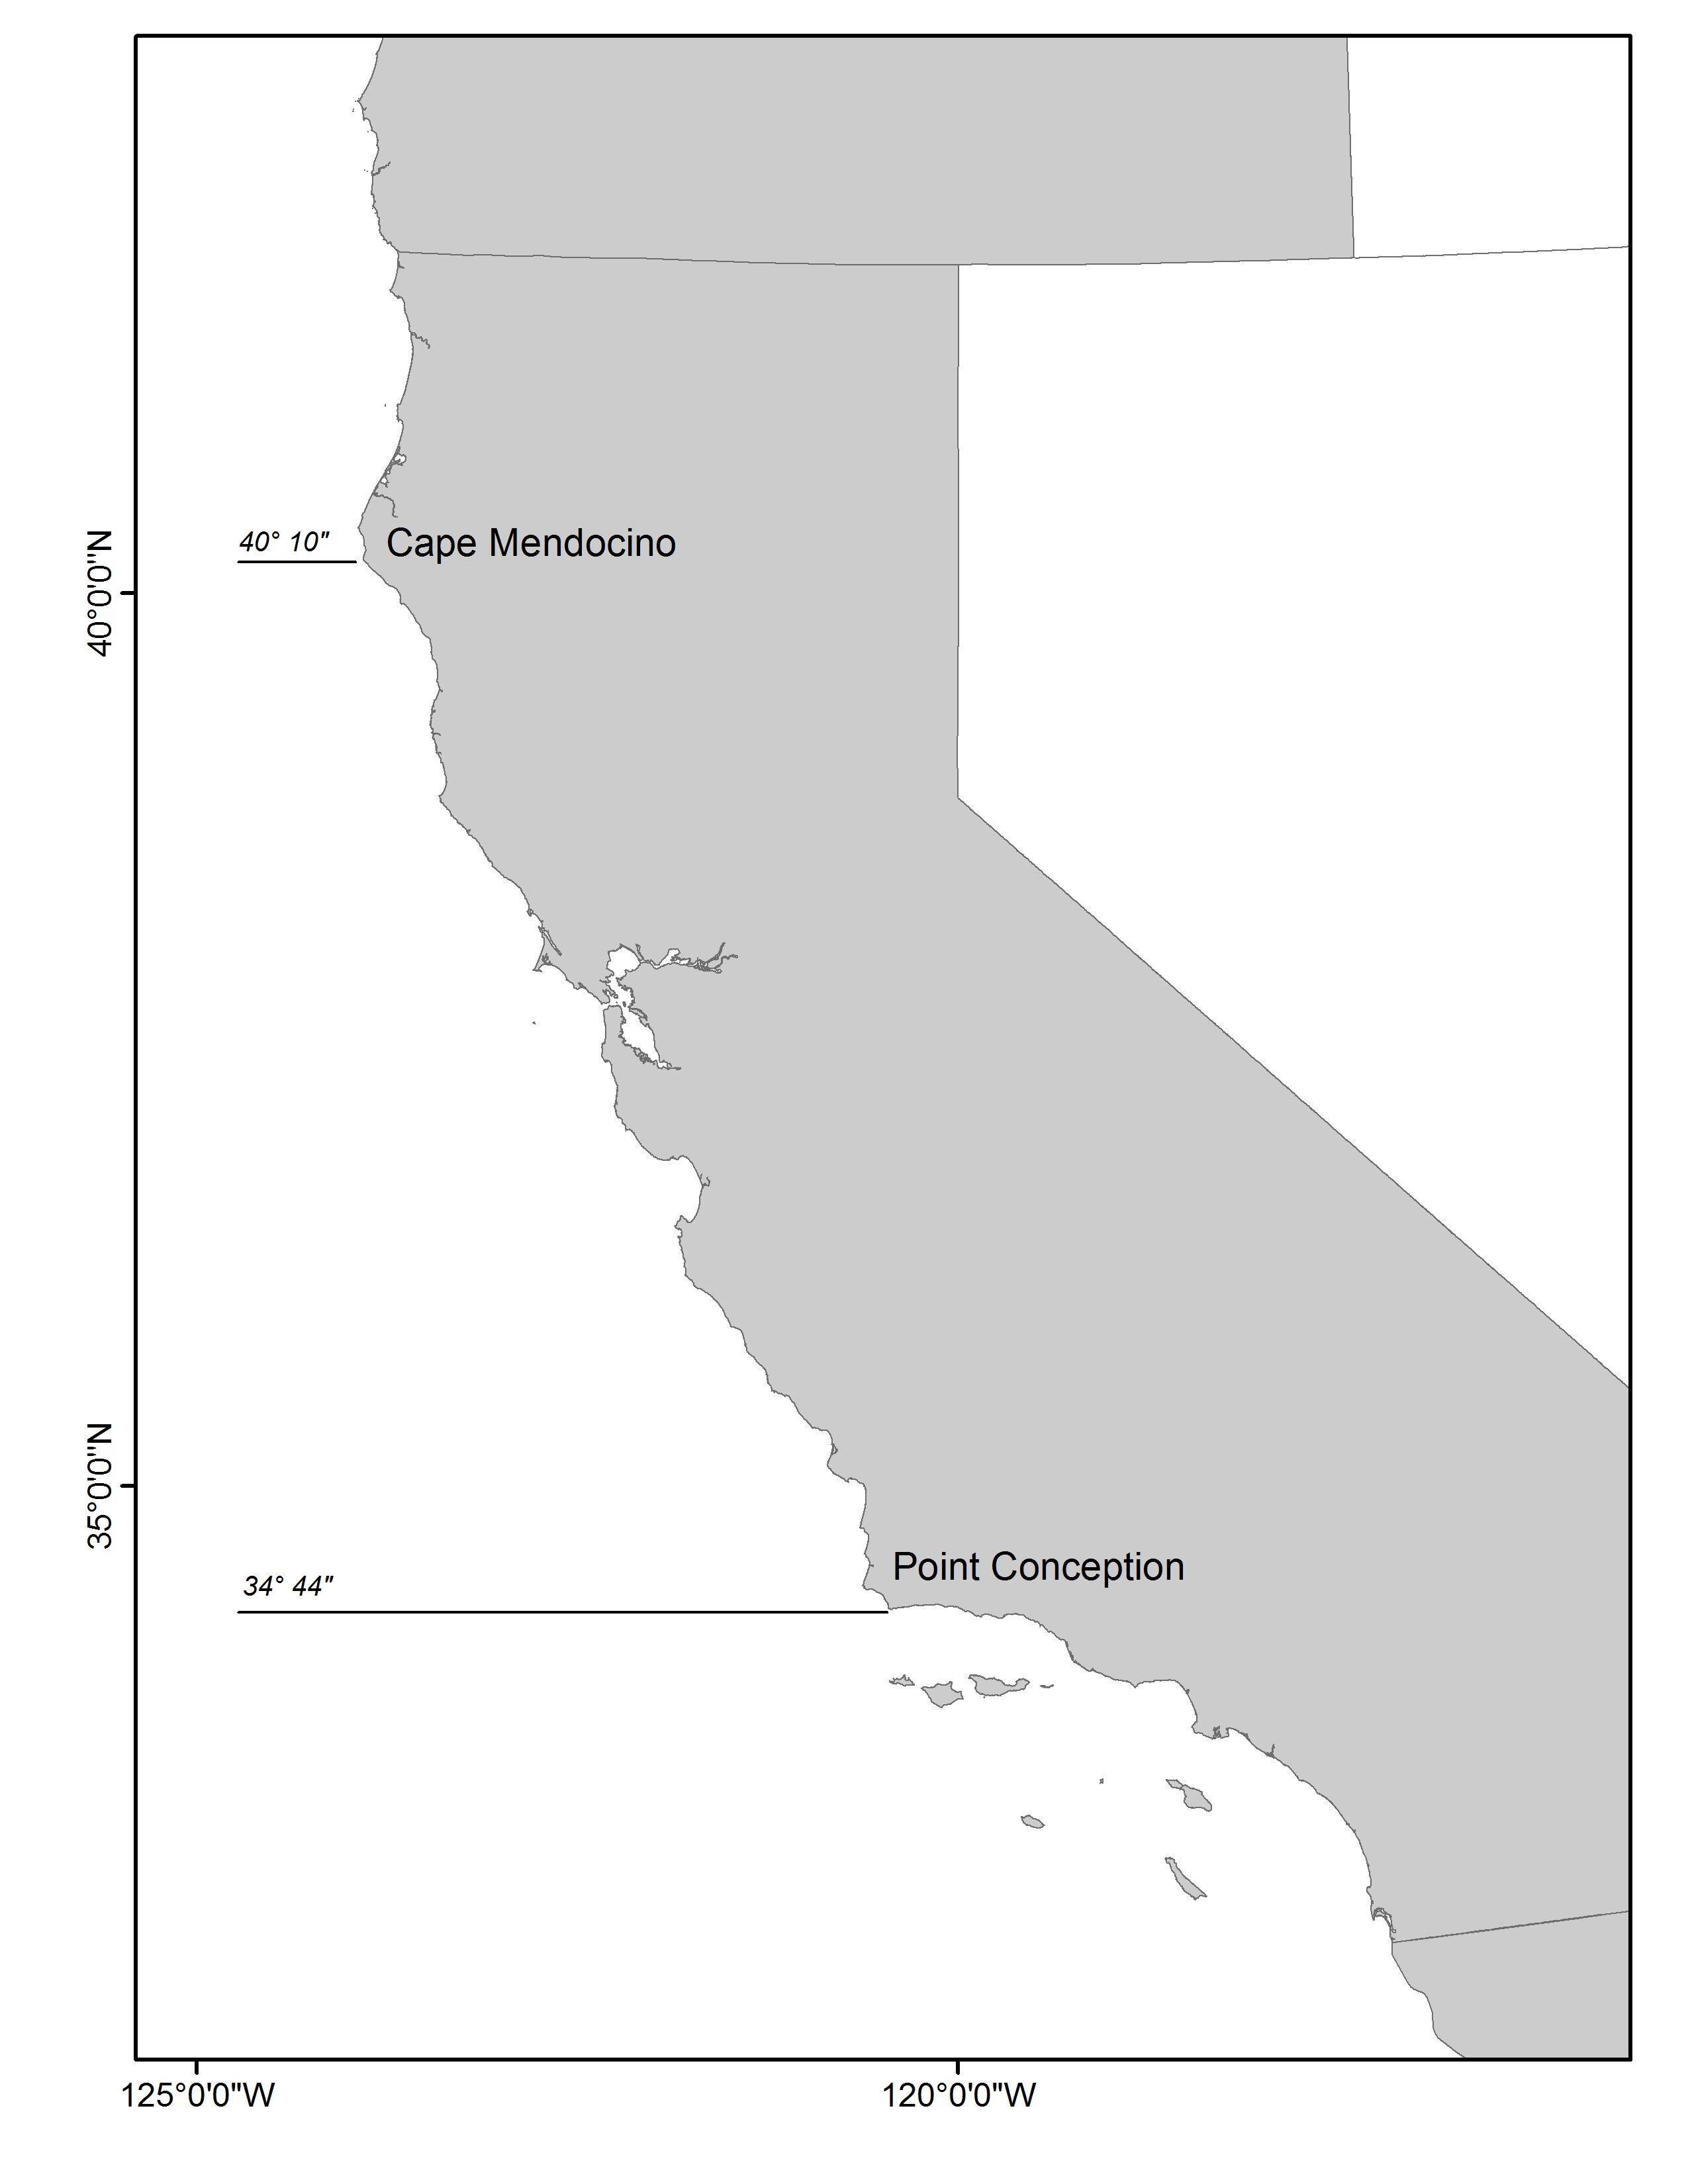
\includegraphics{Figures/assess_region_map.png}
\caption{Map depicting the core distribution of gopher and
black-and-yellow rockfishes. The stock assessment is bounded at Cape
Mendocino in the north to the U.S./Mexico border in the south.
\label{fig:assess_region_map}}
\end{figure}

\FloatBarrier

\subsection*{Stock Biomass}\label{stock-biomass}
\addcontentsline{toc}{subsection}{Stock Biomass}

The predicted spawning output from the base model generally showed a
slight decline prior to 1978, when the recruitment deviations were first
estimated (Figure \ref{fig:Spawnbio_all} and Table
\ref{tab:SpawningDeplete_mod1}). The stock declined from 1978 to 1994,
followed by a period of increase from 1995 to 2003. From 2004-2018 the
stock has been in decline, though increased in total biomass since 2016
and exhibits stable spawning output since from 2018 to 2019. The 2019
estimated spawning output relative to unfished equilibrium spawning
output is above the target of 40\% of unfished spawning output at 43.82
(95\% asymptotic interval: 33.57-54.06) (Figure
\ref{fig:RelDeplete_all}). Approximate confidence intervals based on the
asymptotic variance estimates show that the uncertainty in the estimated
spawning output is high, (95\% asymptotic interval: 337-767 million
eggs). \FloatBarrier

\begin{table}[ht]
\centering
\caption{Recent trend in beginning of the 
                                      year spawning output and depletion for
                                      the model for GBYR.} 
\label{tab:SpawningDeplete_mod1}
\begin{tabular}{l>{\centering}p{1.3in}>{\centering}p{1.2in}>{\centering}p{1in}>{\centering}p{1.3in}}
  \hline
Year & Spawning Output (million eggs) & \~{} 95\% confidence interval & Estimated depletion & \~{} 95\% confidence interval \\ 
  \hline
2010 & 882 & 597 - 1168 & 69.99 & 58.05 - 81.92 \\ 
  2011 & 817 & 548 - 1086 & 64.77 & 53.48 - 76.06 \\ 
  2012 & 761 & 507 - 1014 & 60.33 & 49.63 - 71.03 \\ 
  2013 & 727 & 486 - 968 & 57.66 & 47.5 - 67.81 \\ 
  2014 & 697 & 466 - 928 & 55.31 & 45.56 - 65.05 \\ 
  2015 & 655 & 434 - 877 & 51.98 & 42.4 - 61.55 \\ 
  2016 & 614 & 399 - 828 & 48.69 & 39.16 - 58.22 \\ 
  2017 & 576 & 367 - 786 & 45.70 & 36.12 - 55.28 \\ 
  2018 & 553 & 344 - 762 & 43.85 & 34.08 - 53.63 \\ 
  2019 & 552 & 337 - 767 & 43.82 & 33.57 - 54.06 \\ 
   \hline
\end{tabular}
\end{table}

\FloatBarrier

\begin{figure}
\centering
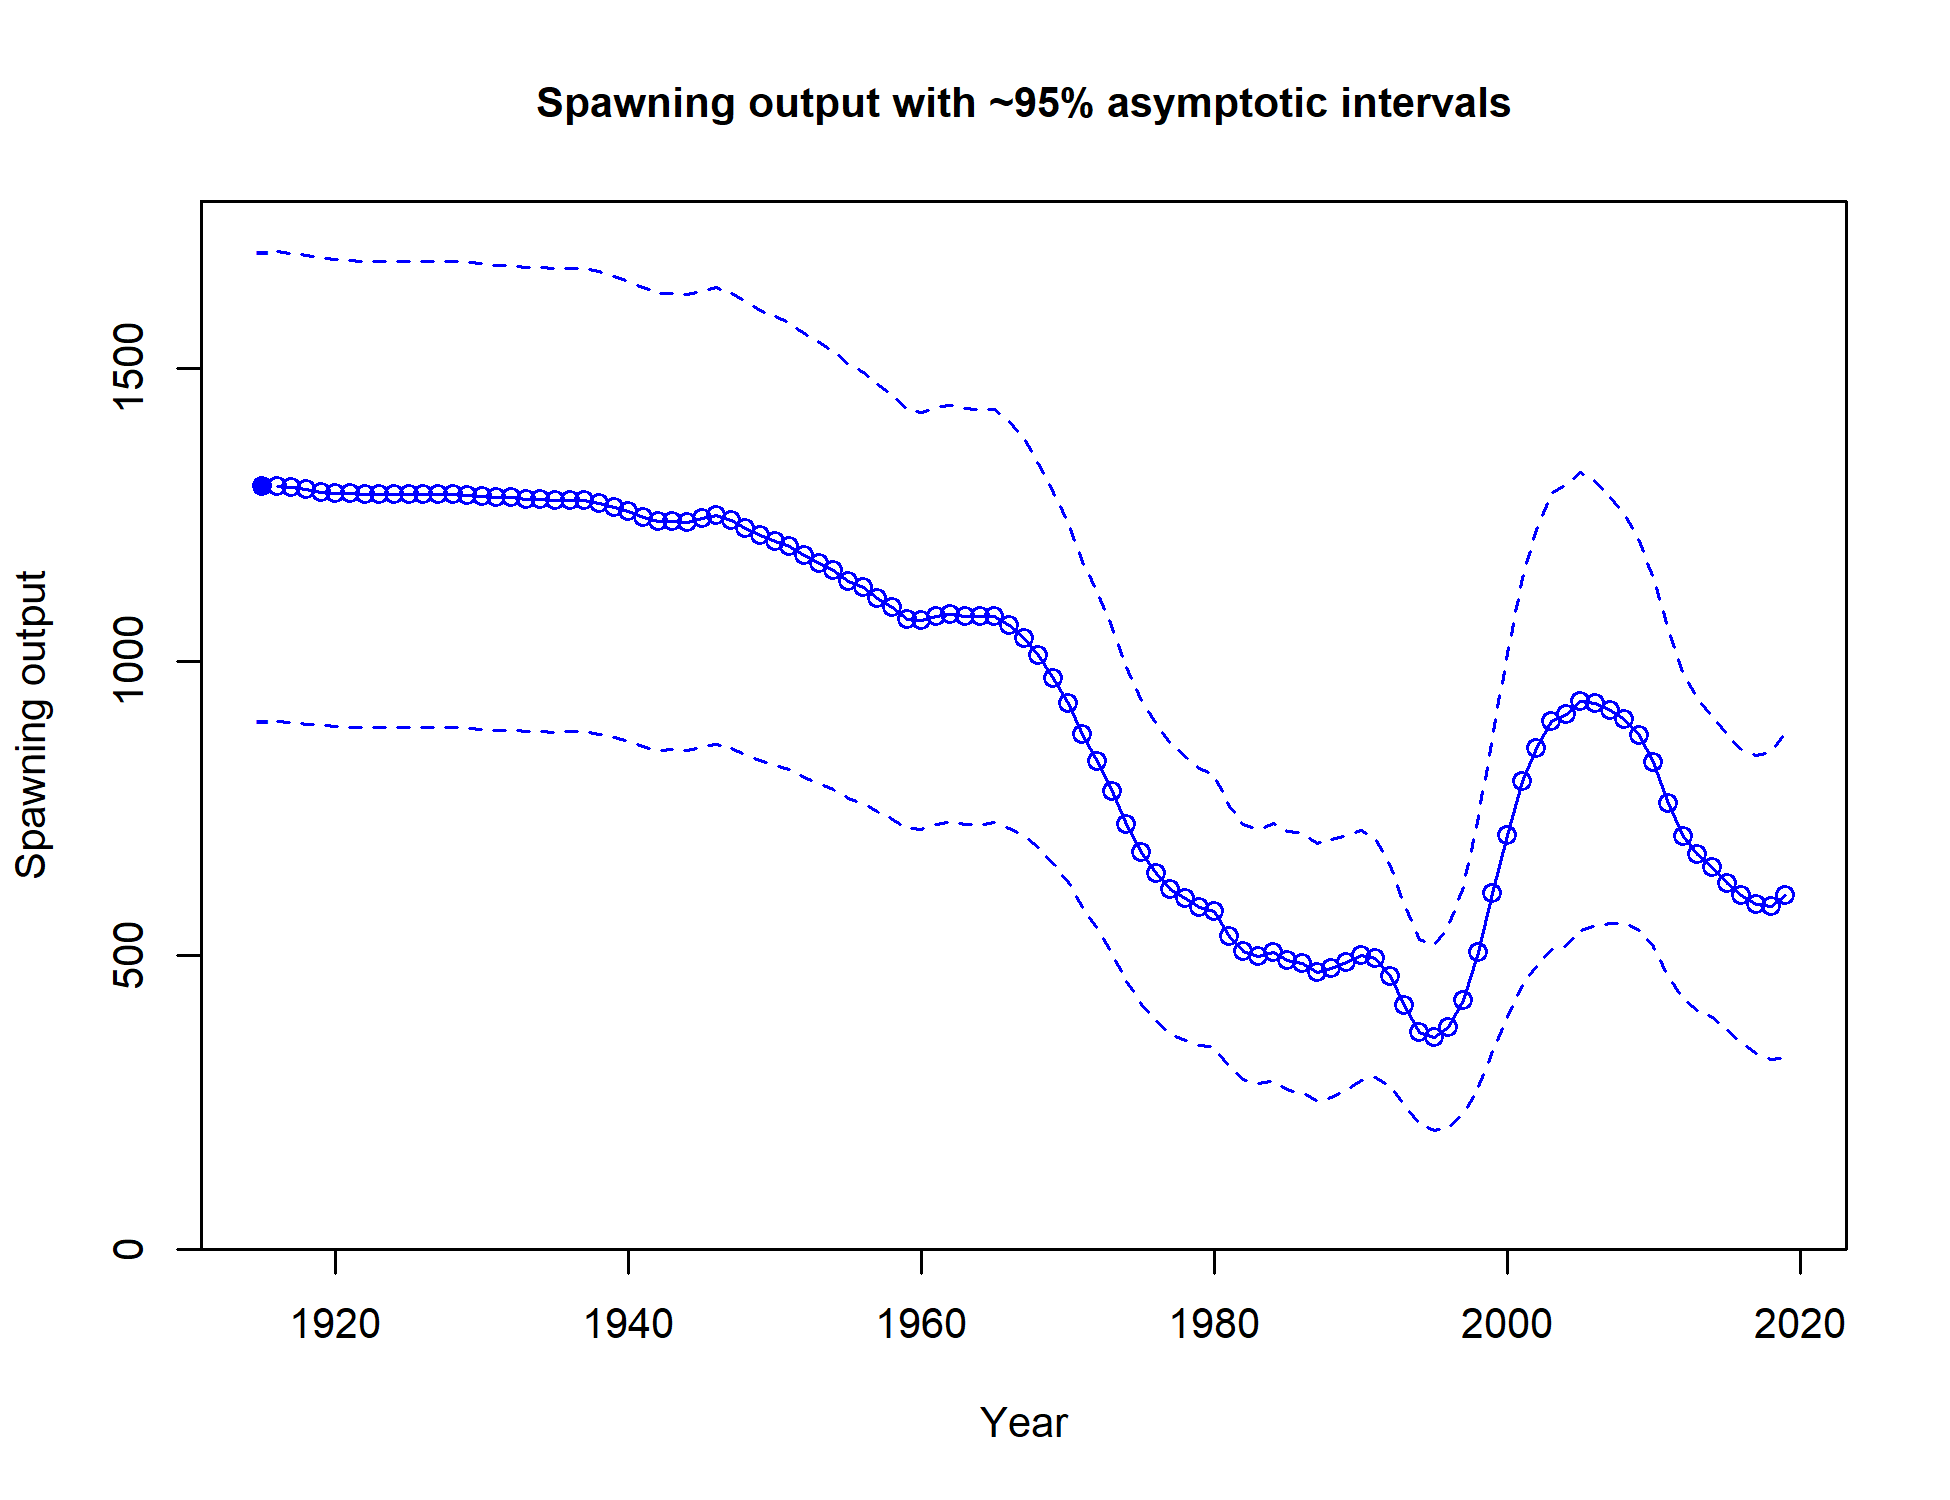
\includegraphics{r4ss/plots_mod1/ts7_Spawning_output_with_95_asymptotic_intervals_intervals.png}
\caption{Time series of spawning output trajectory (circles and line:
median; light broken lines: 95\% credibility intervals) for the base
case assessment model. \label{fig:Spawnbio_all}}
\end{figure}

\begin{figure}
\centering
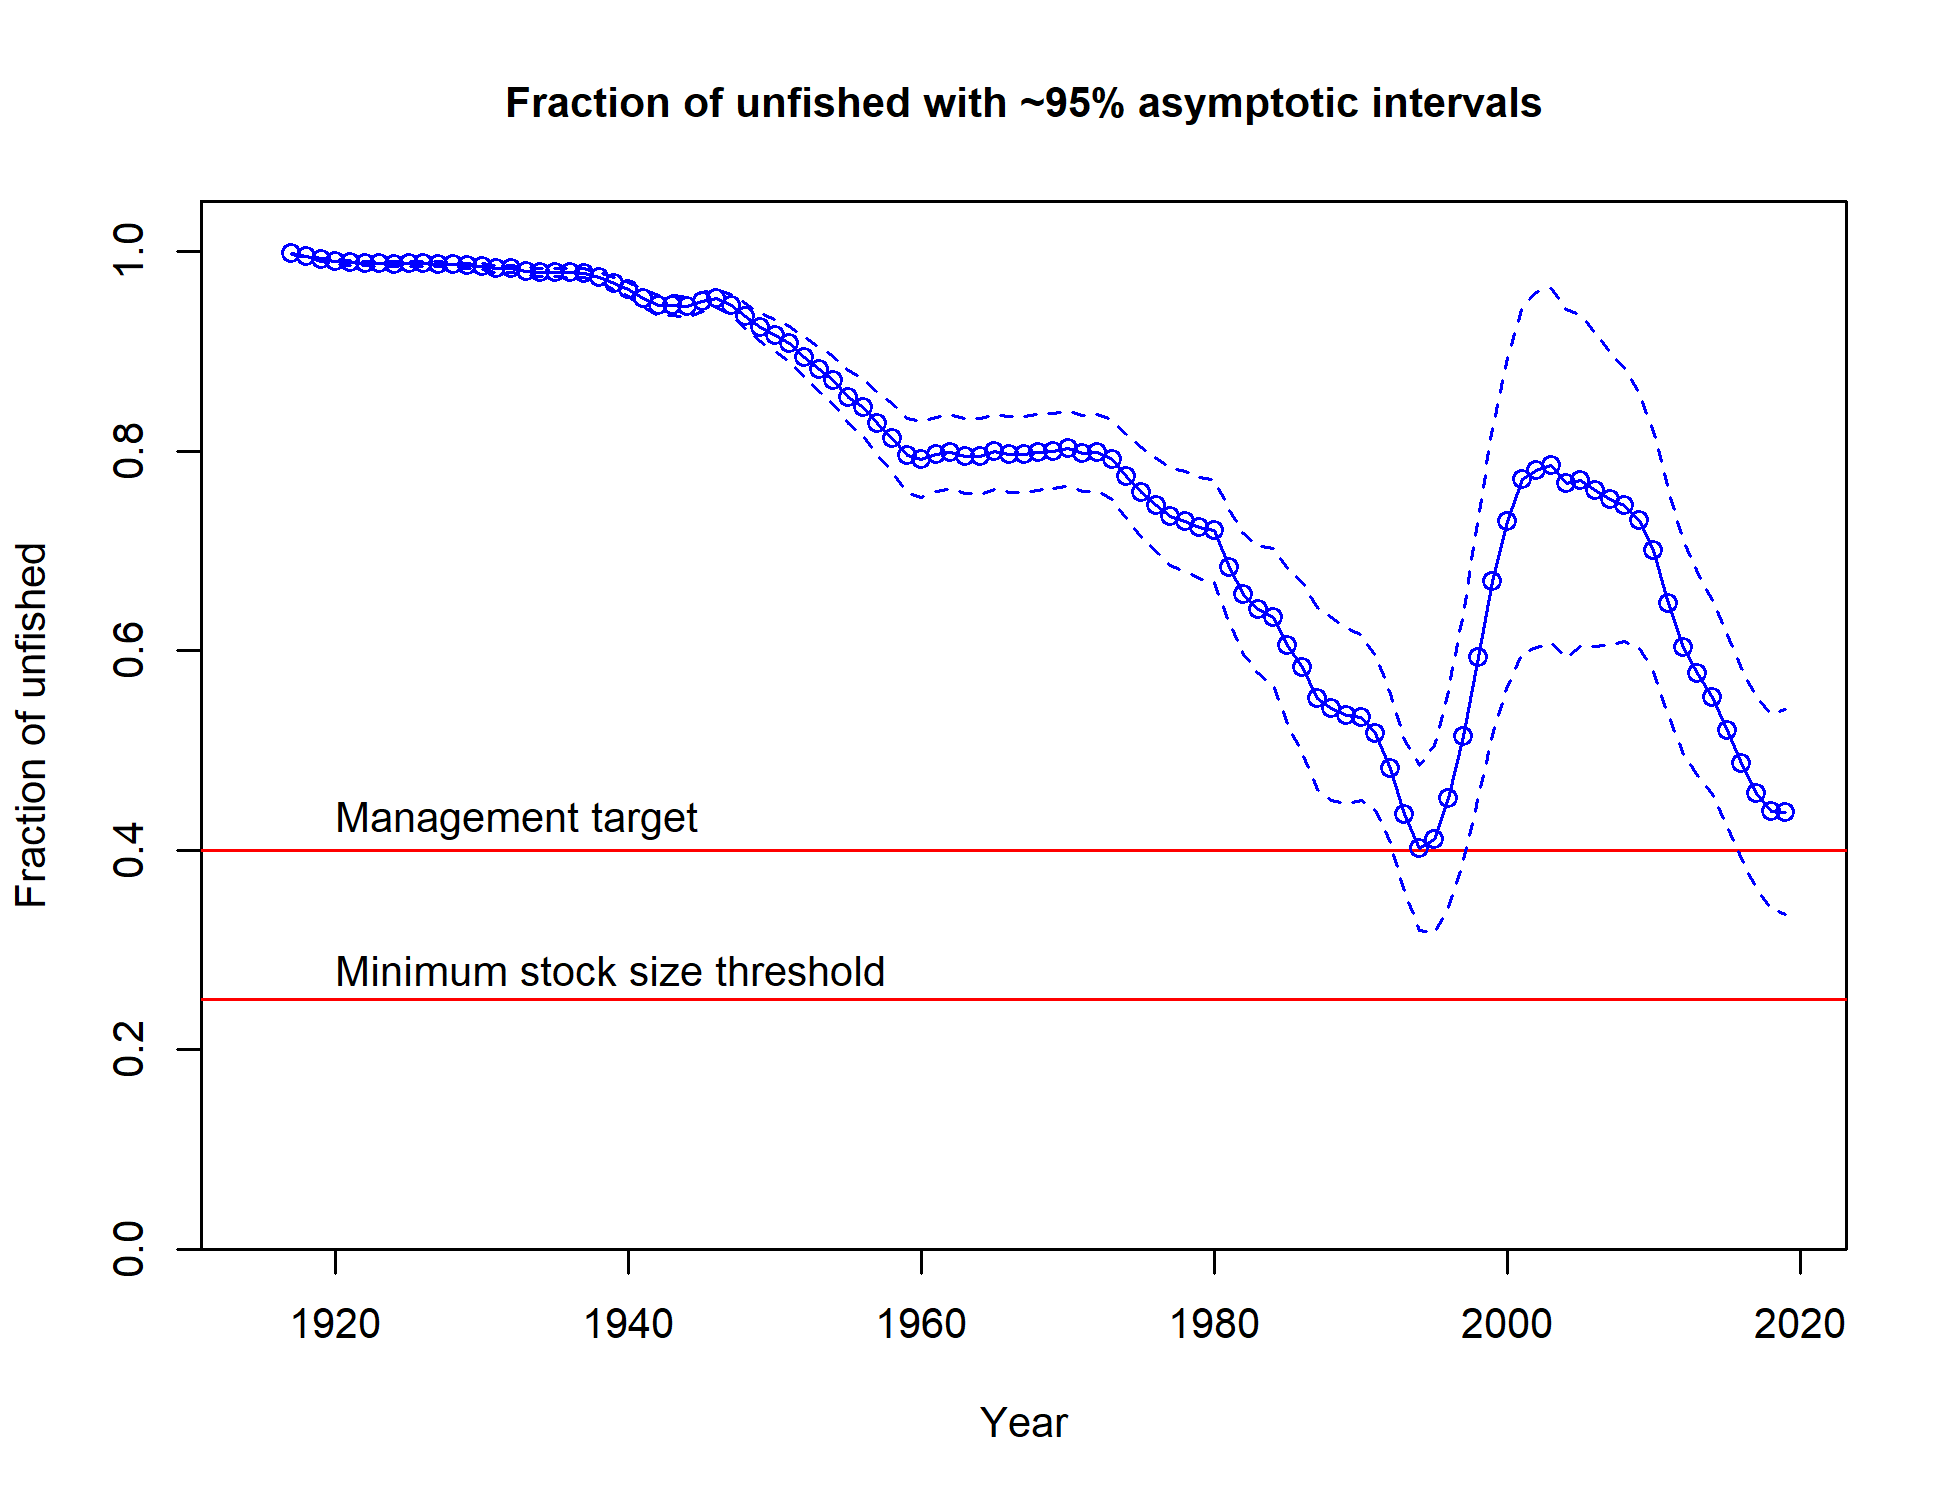
\includegraphics{r4ss/plots_mod1/ts9_Fraction_of_unfished_with_95_asymptotic_intervals_intervals.png}
\caption{Estimated fraction of unfished (percent depletion) with
approximate 95\% asymptotic confidence intervals (dashed lines) for the
base case assessment model. \label{fig:RelDeplete_all}}
\end{figure}

\FloatBarrier

\subsection*{Recruitment}\label{recruitment}
\addcontentsline{toc}{subsection}{Recruitment}

Recruitment deviations were estimated from 1979-2018 (Figure
\ref{fig:Recruits_all} and Table \ref{tab:Recruit_mod1}). There are
estimates of very strong recruitment in 1991, with high recruitment
pulses for a number of other years including 1994-1995 and 2014-2015.

\begin{table}[ht]
\centering
\caption{Recent recruitment for the GBYR assessment.} 
\label{tab:Recruit_mod1}
\begin{tabular}{>{\centering}p{.8in}>{\centering}p{1.6in}>{\centering}p{1.6in}}
  \hline
Year & Estimated Recruitment (1,000s) & \~{} 95\% confidence interval \\ 
  \hline
2010 & 2451 & 1257 - 4779 \\ 
  2011 & 2014 & 983 - 4127 \\ 
  2012 & 1800 & 761 - 4258 \\ 
  2013 & 1589 & 676 - 3734 \\ 
  2014 & 4568 & 2519 - 8284 \\ 
  2015 & 5264 & 2985 - 9282 \\ 
  2016 & 2487 & 1274 - 4857 \\ 
  2017 & 3701 & 1976 - 6935 \\ 
  2018 & 1432 & 664 - 3089 \\ 
  2019 & 2778 & 1086 - 7111 \\ 
   \hline
\end{tabular}
\end{table}

\FloatBarrier

\begin{figure}
\centering
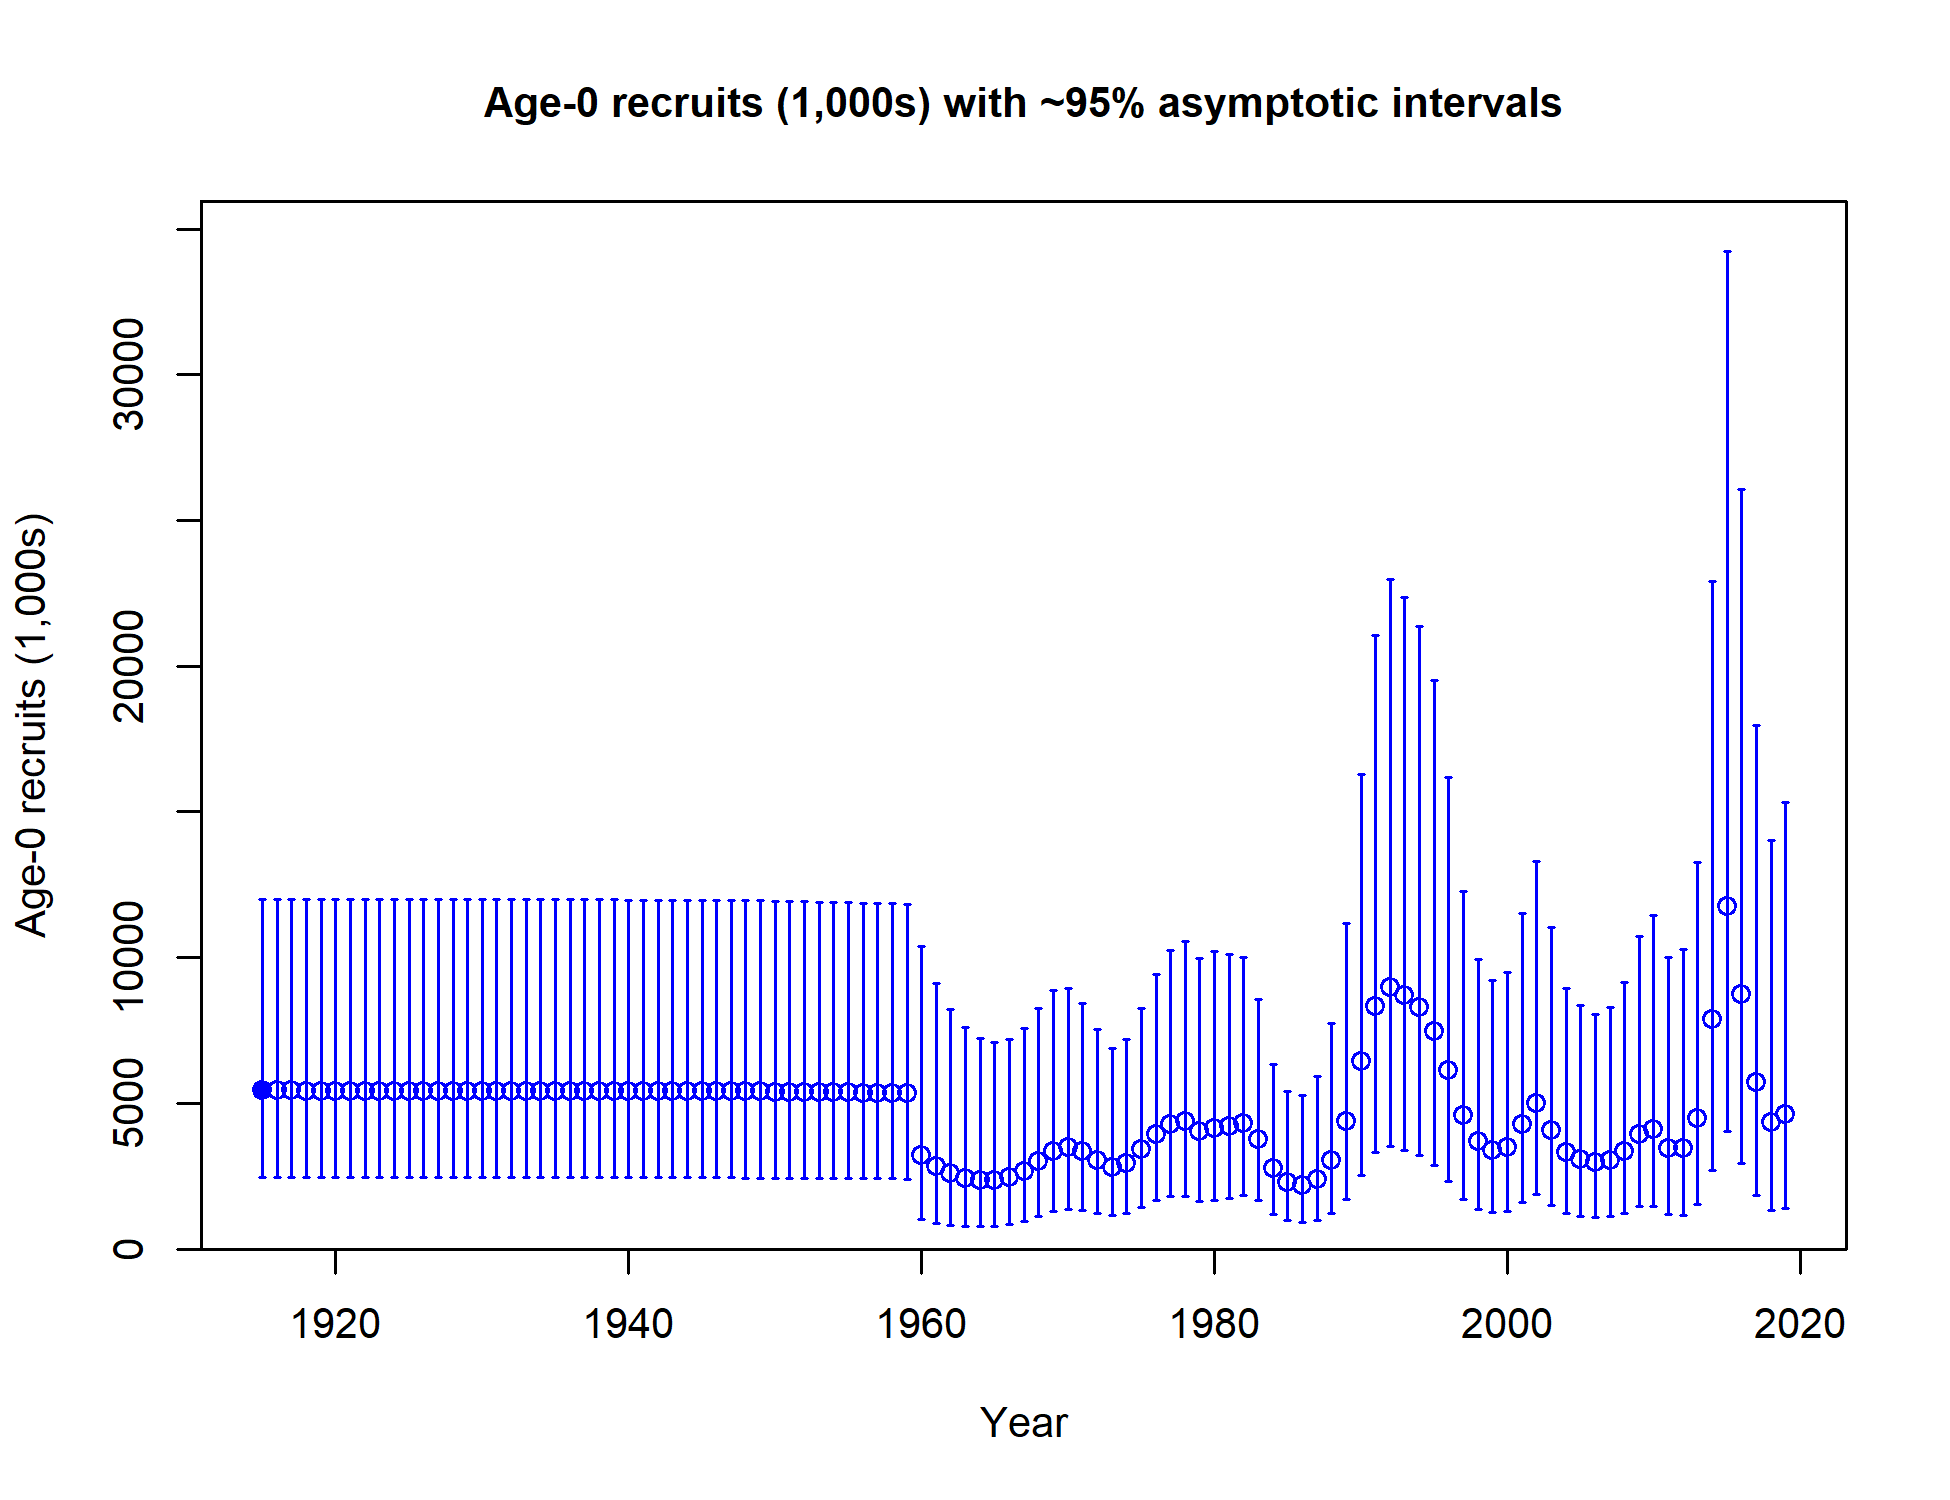
\includegraphics{r4ss/plots_mod1/ts11_Age-0_recruits_(1000s)_with_95_asymptotic_intervals.png}
\caption{Time series of estimated GBYR recruitments for the post-STAR
base model with 95\% confidence or credibility intervals.
\label{fig:Recruits_all}}
\end{figure}

\FloatBarrier

\subsection*{Exploitation status}\label{exploitation-status}
\addcontentsline{toc}{subsection}{Exploitation status}

Harvest rates estimated by the base model indicate catch levels have
been below the limits that would be associated with the Spawning
Potential Ratio (SPR) = 50\% limit (corresponding to a relative fishing
intensity of 100\%) (Table \ref{tab:SPR_Exploit_mod1} and Figure
\ref{fig:SPR_all}). SPR is calculated as the lifetime spawning potential
per recruit at a given fishing level relative to the lifetime spawning
potential per recruit with no fishing. The relative inverse SPR over the
last decade increased ranged from 0.64 to 0.77 from 2009-2015, and
ranged from 0.80 to 0.82 from 2016-2018 (Table
\ref{tab:SPR_Exploit_mod1}).

\FloatBarrier

\begin{table}[ht]
\centering
\caption{Recent trend in spawning potential 
                                        ratio (entered as $(1-SPR)/ (1-SPR_{50\%})$) 
                                        and exploitation for GBYR in the model.} 
\label{tab:SPR_Exploit_mod1}
\begin{tabular}{l>{\centering}p{1.2in}>{\centering}p{1.2in}>{\centering}p{1in}>{\centering}p{1.2in}}
  \hline
Year & Estimated (1-SPR)/(1-SPR50\%) & \~{} 95\% confidence interval & Exploitation rate & 95\% confidence interval \\ 
  \hline
2009 & 0.64 & 0.5 - 0.78 & 0.07 & 0.05 - 0.09 \\ 
  2010 & 0.78 & 0.64 - 0.93 & 0.10 & 0.08 - 0.13 \\ 
  2011 & 0.77 & 0.62 - 0.92 & 0.10 & 0.07 - 0.12 \\ 
  2012 & 0.67 & 0.52 - 0.81 & 0.07 & 0.05 - 0.09 \\ 
  2013 & 0.64 & 0.49 - 0.78 & 0.07 & 0.05 - 0.09 \\ 
  2014 & 0.74 & 0.59 - 0.88 & 0.09 & 0.06 - 0.11 \\ 
  2015 & 0.77 & 0.62 - 0.92 & 0.10 & 0.07 - 0.12 \\ 
  2016 & 0.81 & 0.66 - 0.96 & 0.10 & 0.07 - 0.13 \\ 
  2017 & 0.82 & 0.66 - 0.98 & 0.09 & 0.06 - 0.11 \\ 
  2018 & 0.80 & 0.63 - 0.96 & 0.07 & 0.05 - 0.1 \\ 
   \hline
\end{tabular}
\end{table}

\FloatBarrier

\begin{figure}
\centering
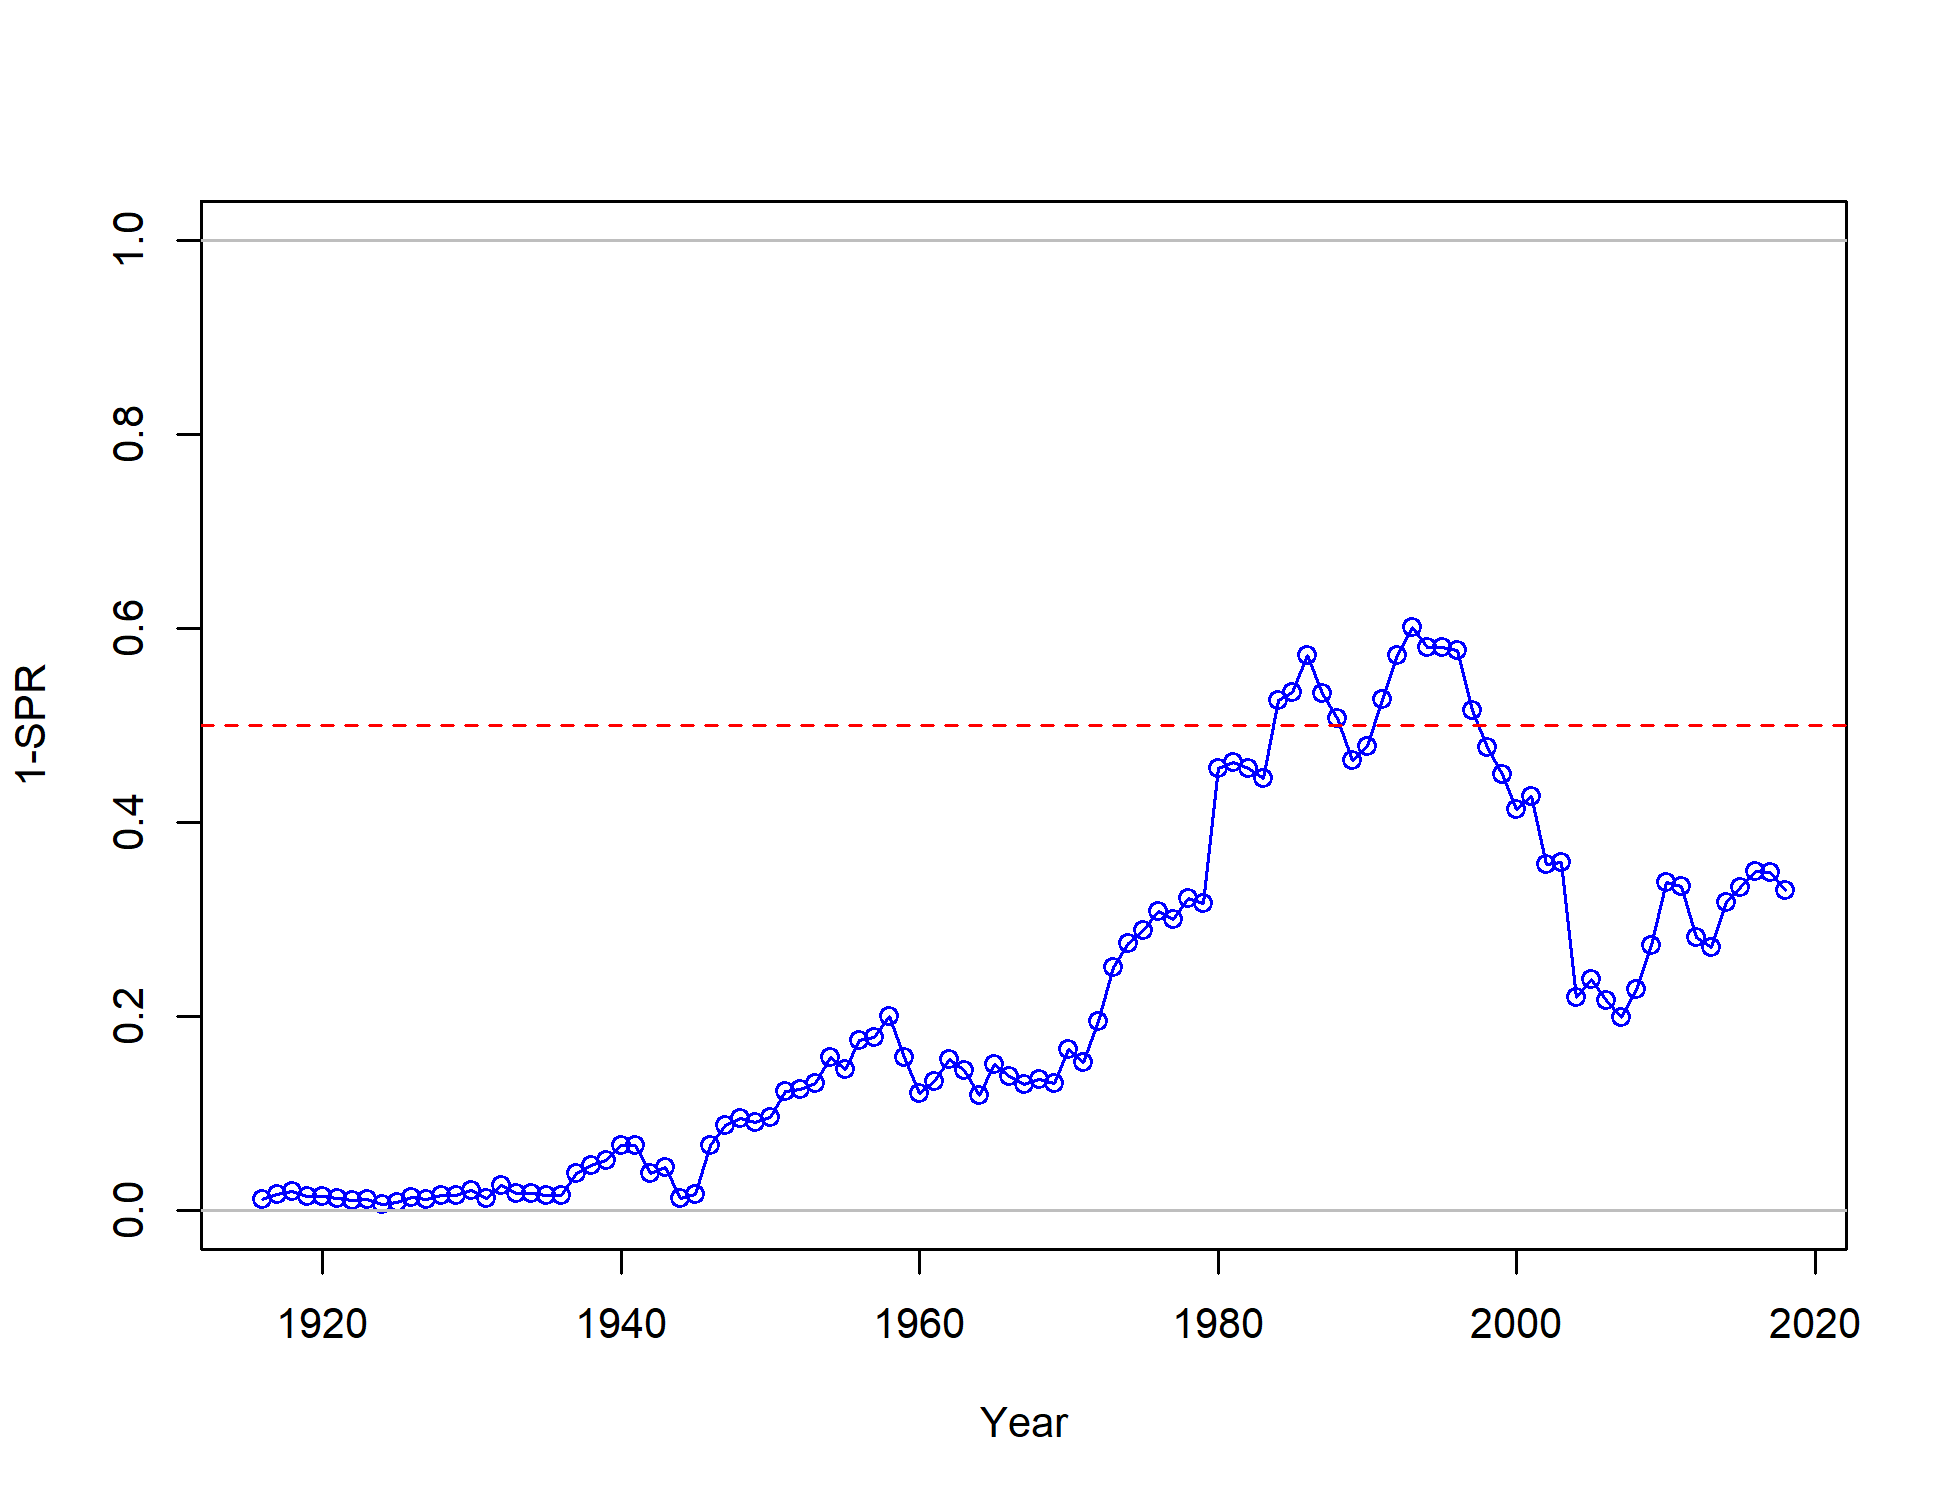
\includegraphics{r4ss/plots_mod1/SPR2_minusSPRseries.png}
\caption{Estimated inverse spawning potential ratio (SPR) for the
post-STAR base model, plotted as one minus SPR so that higher
exploitation rates occur on the upper portion of the y-axis. The
management target is plotted as a red horizontal line and values above
this reflect harvests in excess of the overfishing proxy based on the
SPR\textsubscript{50\%} harvest rate. The last year in the time series
is 2018. \label{fig:SPR_all}}
\end{figure}

\FloatBarrier

\subsection*{Ecosystem Considerations}\label{ecosystem-considerations}
\addcontentsline{toc}{subsection}{Ecosystem Considerations}

In this assessment, ecosystem considerations were not explicitly
included in the analysis.\\
This is primarily due to a lack of relevant data and results of analyses
(conducted elsewhere) that could contribute ecosystem-related
quantitative information for the assessment.

\subsection*{Reference Points}\label{reference-points}
\addcontentsline{toc}{subsection}{Reference Points}

This stock assessment estimates that GBYR in the model is above the
biomass target (\(SB_{40\%}\)), and well above the minimum stock size
threshold (\(SB_{25\%}\)). The estimated relative depletion level for
the base model in 2018 is 0.439 (95\% asymptotic interval: 0.341-0.536,
corresponding to an unfished spawning of 552 million eggs (95\%
asymptotic interval: 337 - 767 million eggs) of spawning output in the
base model (Table \ref{tab:Ref_pts_mod1}). Unfished age 1+ biomass was
estimated to be 2,042 mt in the base case model. The target spawning
output (\(SB_{40\%}\)) is 504 million eggs, which corresponds with an
equilibrium yield of 143 mt. Equilibrium yield at the proxy \(F_{MSY}\)
harvest rate corresponding to \(SPR_{50\%}\) is 134 mt (Figure
\ref{fig:Yield_all}).

\FloatBarrier

\begin{table}[ht]
\centering
\caption{Summary of reference 
                                      points and management quantities for the 
                                      base case model.} 
\label{tab:Ref_pts_mod1}
\begin{tabular}{>{\raggedright}p{4.1in}>{\raggedleft}p{.62in}>{\raggedleft}p{.62in}>{\raggedleft}p{.62in}}
  \hline
\textbf{Quantity} & \textbf{Estimate} & \textbf{Low 2.5\%  limit} & \textbf{High 2.5\%  limit} \\ 
  \hline
Unfished spawning output (million eggs) & 1,261 & 968 & 1,554 \\ 
  Unfished age 1+ biomass (mt) & 2,042 & 1,637 & 2,448 \\ 
  Unfished recruitment ($R_{0}$) & 3,125 & 2,643 & 3,606 \\ 
  Spawning output (2018 million eggs) & 553 & 344 & 762 \\ 
  Depletion (2018) & 0.439 & 0.341 & 0.536 \\ 
  \textbf{$\text{Reference points based on } \mathbf{SB_{40\%}}$} &  &  &  \\ 
  Proxy spawning output ($B_{40\%}$) & 504 & 427 & 582 \\ 
  SPR resulting in $B_{40\%}$ ($SPR_{B40\%}$) & 0.458 & 0.458 & 0.458 \\ 
  Exploitation rate resulting in $B_{40\%}$ & 0.126 & 0.109 & 0.144 \\ 
  Yield with $SPR_{B40\%}$ at $B_{40\%}$ (mt) & 143 & 124 & 162 \\ 
  \textbf{\textit{Reference points based on SPR proxy for MSY}} &  &  &  \\ 
  Spawning output & 563 & 476 & 649 \\ 
  $SPR_{proxy}$ & 0.5 &  &  \\ 
  Exploitation rate corresponding to $SPR_{proxy}$ & 0.111 & 0.096 & 0.126 \\ 
  Yield with $SPR_{proxy}$ at $SB_{SPR}$ (mt) & 134 & 116 & 152 \\ 
  \textbf{\textit{Reference points based on estimated MSY values}} &  &  &  \\ 
  Spawning output at $MSY$ ($SB_{MSY}$) & 281 & 235 & 328 \\ 
  $SPR_{MSY}$ & 0.299 & 0.29 & 0.308 \\ 
  Exploitation rate at $MSY$ & 0.209 & 0.174 & 0.244 \\ 
  Dead Catch $MSY$ (mt) & 163 & 141 & 185 \\ 
  Retained Catch $MSY$ (mt) & 163 & 141 & 185 \\ 
   \hline
\end{tabular}
\end{table}

\FloatBarrier

\subsection*{Management Performance}\label{management-performance}
\addcontentsline{toc}{subsection}{Management Performance}

Gopher and black-and-yellow rockfishes are managed as part of the minor
nearshore complex in the Pacific Coast Groundfish Fishery Management
Plan. The total mortality of the minor nearshore rockfish has been below
the ACL in all years (2011-2016). Total mortality estimates from the
NWFSC are not yet available for 2017-2018. GBYR total mortality was on
average 20\% of the total minor nearshore rockfish total mortality from
2011-2016. A summary of these values as well as other base case summary
results can be found in Table \ref{tab:mnmgt_perform}.

\begin{table}[ht]
\centering
\caption{Recent trend in total mortality for gopher and 
                            black-and-yellow rockfishes (GBYR), combined, relative to the 
                             management guidelines for Nearshore Rockfish 
                             South of $40^\circ 10^\prime$ N. latitude. 
                             Total mortality estimates are based on annual reports 
                                from the NMFS NWFSC.} 
\label{tab:mnmgt_perform}
\begin{tabular}{lllll}
  \hline
   \multicolumn{1}{c}{} & \multicolumn{1}{c}{GBYR} & \multicolumn{1}{c}{Shallow Nearshore Rockfish South} & \multicolumn{2}{c}{Nearshore Rockfish South} \\  \cmidrule(lr){2-2} \cmidrule(lr){3-3} \cmidrule(lr){4-5}
   \hline
Year & Total mortality & Total mortality & ACL & OFL \\ 
  \hline
\textbf{2011} & 122.87 & 436 & 1,001 & 1,156 \\ 
  \textbf{2012} & 91.96 & 445 & 1,001 & 1,145 \\ 
  \textbf{2013} & 104.53 & 495 & 990 & 1,164 \\ 
  \textbf{2014} & 103.63 & 596 & 990 & 1,160 \\ 
  \textbf{2015} & 107.95 & 676 & 1,114 & 1,313 \\ 
  \textbf{2016} & 111.55 & 641 & 1,006 & 1,288 \\ 
  \textbf{2017} & - & - & 1,163 & 1,329 \\ 
  \textbf{2018} & - & - & 1,179 & 1,344 \\ 
   \hline
   \hline
\end{tabular}
\end{table}

\FloatBarrier

\subsection*{Unresolved Problems and Major
Uncertainties}\label{unresolved-problems-and-major-uncertainties}
\addcontentsline{toc}{subsection}{Unresolved Problems and Major
Uncertainties}

The major source of uncertainty identified during the STAR panel are the
structure of two species complex, the contribution of each of the two
species to the complex, and differences in biological parameters between
the species. There is currently no information for either species on
regional differences in biological parameters and contributions to the
complex.

\FloatBarrier

\subsection*{Decision Table}\label{decision-table}
\addcontentsline{toc}{subsection}{Decision Table}

The forecasts of stock abundance and yield were developed using the
post-STAR base model, with the forecasted projections of the OFL
presented in Table \ref{tab:OFL_projection}. The total catches in 2019
and 2020 are set to the projected catch from the California Department
of Fish and Wildlife (CDFW) of 114 mt.

Uncertainty in the forecasts is based upon the three states of nature
agreed upon at the STAR panel and are based three states of nature of
growth. The external estimate of growth was different than the internal
Stock Synthesis estimate. Given that natural mortality is fixed in the
post-STAR base model, and the growth parameter \(k\) is negatively
correlated with natural mortality, \(k\) was chosen as the axis of
uncertainty. The high state of nature fixes \(k\) at the external
estimate, and the low state of nature is the same distance in log space
from the base as the high state of nature. The low state of nature fixed
\(k\) at 0.046 and the L1 and L1 parameters were estimated at 14.1 and
30.6, respectively. The high state of nature fixed all growth
parameters, \(k\) = 0.248, L1 = 13.8, and L2 = 28.5 to the external
estimate of growth (due to improbable estimates of L1 and L2 if only
\(k\) was fixed to the external estimate). The growth parameters in the
base model were estimated as \(k\) = 0.107, L1 = 13.4, and L2 = 28.8.

The forecasted buffer ramp was calculated assuming a category 2 stock,
with sigma = 1.0 and a \(p^*\) = 0.45. The buffer ranges from 0.874 in
2021 ramping to 0.803 in 2030. For reference, the model predicted sigma
is 0.189 and the decision table-based sigma is 0.197. Current
medium-term forecasts based on the alternative states of nature project
that the stock will remain above the target threshold of 40\% for all
but two scenarios (Table \ref{tab:Decision_table_mod1}). The low state
of nature with the high catches results in a stock at 26.4\% of unfished
in 2030 and the base state model with the high catches results in a
stock at 33.2\% of unfished in 2030. The base case model with the base
catches results in an increasing stock over the period from 2021-2030.
If the growth of GBYR is slower than the base model suggests, but the
base case catches are removed, the stock will be at the target threshold
in 2030.

\begin{table}[ht]
\centering
\caption{Projected OFL, default harvest control rule 
                                        catch (ABC = ACL) above 40\% SSB, biomass, 
                                        and depletion using the post-STAR base case model with 
                                        2019-2020 catches set equal to the projected catch 
                                        (114 mt) rather than the ABC.} 
\label{tab:OFL_projection}
\begin{tabular}{cc>{\centering}p{.9in}>{\centering}p{1in}>{\centering}p{1in}>{\centering}p{1in}}
  \hline
Year & OFL (mt) & ABC Catch (mt) & Age 0+ Biomass (mt) & Spawning Output (million eggs) &  Fraction unfished \\ 
  \hline
2019 & 154 & \textit{114} & 1281 & 552.5 & 43.8 \\ 
  2020 & 154 & \textit{114} & 1292 & 558.3 & 44.3 \\ 
  2021 & 136 & 119 & 1291 & 578.2 & 45.9 \\ 
  2022 & 137 & 119 & 1296 & 601.1 & 47.7 \\ 
  2023 & 143 & 122 & 1300 & 621.5 & 49.3 \\ 
  2024 & 150 & 127 & 1302 & 633.3 & 50.2 \\ 
  2025 & 155 & 130 & 1300 & 636.2 & 50.5 \\ 
  2026 & 158 & 131 & 1295 & 632.6 & 50.2 \\ 
  2027 & 158 & 130 & 1290 & 626.0 & 49.7 \\ 
  2028 & 156 & 128 & 1286 & 619.4 & 49.1 \\ 
  2029 & 155 & 125 & 1284 & 614.8 & 48.8 \\ 
  2030 & 153 & 123 & 1283 & 612.7 & 48.6 \\ 
   \hline
\end{tabular}
\end{table}\begin{table}[ht]
\centering
\caption{Summary of 10-year 
                                             projections beginning in 2020 
                                             for alternate states of nature based on 
                                             an axis of uncertainty for the model.  Columns range over low, mid, and high
                                             states of nature, and rows range over different 
                                             assumptions of catch levels. The low state of nature 
                                             fixed the growth parameter $k$ at 0.046 and the high 
                                             state fixes all growth parameters to the external 
                                             estimate ($k$ = 0.248, L1 = 13.8, L2 = 28.5). For reference 
                                             the base case estimated $k$ = 0.106, L1 = 13.4 and L2 = 28.9. 
                                            The 2019 and 2020 catches were set to the projected catch of 
                                              114 mt, provided by CDFW.} 
\label{tab:Decision_table_mod1}
\scalebox{0.85}{
\begin{tabular}{l|cc|>{\centering}p{.7in}c|>{\centering}p{.7in}c|>{\centering}p{.7in}c}
   \multicolumn{3}{c}{}  &  \multicolumn{2}{c}{} 
                               & \multicolumn{2}{c}{\textbf{States of nature}} 
                               & \multicolumn{2}{c}{} \\
  \multicolumn{3}{c}{}  &  \multicolumn{2}{c}{Low State} 
                               & \multicolumn{2}{c}{Base State} 
                               &  \multicolumn{2}{c}{High State} \\
 \hline
 & Year & Catch & Spawning Output & Depletion & Spawning Output & Depletion & Spawning Output & Depletion \\ 
  \hline
 & 2019 & 114 & 444.4 & 37.3 & 552.5 & 43.8 & 1105.4 & 58.5 \\ 
   & 2020 & 114 & 443.3 & 37.2 & 558.3 & 44.3 & 1168.8 & 61.9 \\ 
   & 2021 & 75 & 449.6 & 37.7 & 578.2 & 45.9 & 1231.2 & 65.2 \\ 
   & 2022 & 80 & 481.2 & 40.4 & 623.4 & 49.4 & 1296.5 & 68.6 \\ 
  Default harvest & 2023 & 85 & 510.4 & 42.8 & 660.8 & 52.4 & 1322.9 & 70.0 \\ 
  for Low State & 2024 & 91 & 534.5 & 44.9 & 687.1 & 54.5 & 1329.1 & 70.4 \\ 
   & 2025 & 96 & 552.0 & 46.3 & 702.5 & 55.7 & 1328.9 & 70.4 \\ 
   & 2026 & 101 & 562.5 & 47.2 & 709.3 & 56.3 & 1326.8 & 70.2 \\ 
   & 2027 & 104 & 567.1 & 47.6 & 710.4 & 56.3 & 1324.2 & 70.1 \\ 
   & 2028 & 105 & 567.5 & 47.6 & 708.5 & 56.2 & 1321.7 & 70.0 \\ 
   & 2029 & 105 & 565.8 & 47.5 & 706.1 & 56.0 & 1320.3 & 69.9 \\ 
   & 2030 & 104 & 563.8 & 47.3 & 704.8 & 55.9 & 1320.2 & 69.9 \\ 
   \hline
 & 2019 & 114 & 444.4 & 37.3 & 552.5 & 43.8 & 1105.4 & 58.5 \\ 
   & 2020 & 114 & 443.3 & 37.2 & 558.3 & 44.3 & 1168.8 & 61.9 \\ 
   & 2021 & 119 & 449.6 & 37.7 & 578.2 & 45.9 & 1231.2 & 65.2 \\ 
   & 2022 & 119 & 460.9 & 38.7 & 601.1 & 47.7 & 1267.4 & 67.1 \\ 
  Default harvest & 2023 & 122 & 475.0 & 39.9 & 621.5 & 49.3 & 1270.6 & 67.3 \\ 
  for Base State & 2024 & 127 & 486.5 & 40.8 & 633.3 & 50.2 & 1257.1 & 66.6 \\ 
   & 2025 & 130 & 492.9 & 41.4 & 636.2 & 50.5 & 1240.8 & 65.7 \\ 
   & 2026 & 131 & 493.9 & 41.5 & 632.6 & 50.2 & 1226.6 & 64.9 \\ 
   & 2027 & 130 & 490.8 & 41.2 & 626.0 & 49.7 & 1216.1 & 64.4 \\ 
   & 2028 & 128 & 485.6 & 40.8 & 619.4 & 49.1 & 1209.7 & 64.0 \\ 
   & 2029 & 125 & 480.5 & 40.3 & 614.8 & 48.8 & 1207.0 & 63.9 \\ 
   & 2030 & 123 & 476.8 & 40.0 & 612.7 & 48.6 & 1207.2 & 63.9 \\ 
   \hline
 & 2019 & 114 & 444.4 & 37.3 & 552.5 & 43.8 & 1105.4 & 58.5 \\ 
   & 202 & 114 & 443.3 & 37.2 & 558.3 & 44.3 & 1168.8 & 61.9 \\ 
   & 2021 & 235 & 449.6 & 37.7 & 578.2 & 45.9 & 1231.2 & 65.2 \\ 
   & 2022 & 225 & 410.9 & 34.5 & 544.4 & 43.2 & 1191.3 & 63.1 \\ 
  Default harvest & 2023 & 215 & 390.6 & 32.8 & 522.5 & 41.4 & 1132.0 & 59.9 \\ 
  for High State & 2024 & 204 & 377.9 & 31.7 & 503.3 & 39.9 & 1071.8 & 56.7 \\ 
   & 2025 & 192 & 366.0 & 30.7 & 484.2 & 38.4 & 1025.9 & 54.3 \\ 
   & 2026 & 183 & 353.2 & 29.7 & 466.5 & 37.0 & 996.7 & 52.8 \\ 
   & 2027 & 177 & 340.4 & 28.6 & 451.7 & 35.8 & 980.5 & 51.9 \\ 
   & 2028 & 173 & 328.9 & 27.6 & 440.7 & 34.9 & 972.2 & 51.5 \\ 
   & 2029 & 170 & 320.2 & 26.9 & 433.5 & 34.4 & 968.2 & 51.3 \\ 
   & 2030 & 168 & 314.3 & 26.4 & 429.2 & 34.0 & 966.0 & 51.1 \\ 
   \hline
\end{tabular}
}
\end{table}

\begin{sidewaystable}[ht]
\centering
\caption{Base case results summary.} 
\label{tab:base_summary}
\scalebox{0.6}{
\begin{tabular}{r>{\centering}p{1.1in}>{\centering}p{1.1in}>{\centering}p{1.1in}>{\centering}p{1.1in}>{\centering}p{1.1in}>{\centering}p{1.1in}>{\centering}p{1.1in}>{\centering}p{1.1in}>{\centering}p{1.1in}>{\centering}p{1.1in}}
  \hline
Quantity & 2010 & 2011 & 2012 & 2013 & 2014 & 2015 & 2016 & 2017 & 2018 & 2019 \\ 
  \hline
Total mortality (mt) & 153 & 135 &  94 &  84 & 105 & 109 & 112 & 104 &  92 &  \\ 
  Complex OFL (mt) &  & 1,156 & 1,145 & 1,164 & 1,160 & 1,313 & 1,288 & 1,329 & 1,344 &  \\ 
  Complex ACL (mt) &  & 1,001 & 1,001 & 990 & 990 & 1,114 & 1,006 & 1,163 & 1,179 &  \\ 
  (1-$SPR$)(1-$SPR_{50\%}$) & 0.78 & 0.77 & 0.67 & 0.64 & 0.74 & 0.77 & 0.81 & 0.82 & 0.80 &  \\ 
   \hline
Exploitation rate & 0.10 & 0.10 & 0.07 & 0.07 & 0.09 & 0.10 & 0.10 & 0.09 & 0.07 &  \\ 
   \hline
Age 1+ biomass (mt) & 1550.00 & 1469.27 & 1364.64 & 1283.44 & 1238.94 & 1196.76 & 1148.01 & 1143.82 & 1190.26 & 1237.83 \\ 
  Spawning Output & 882 & 817 & 761 & 727 & 697 & 655 & 614 & 576 & 553 & 552 \\ 
   \hline
~95\% CI & 597 - 1168 & 548 - 1086 & 507 - 1014 & 486 - 968 & 466 - 928 & 434 - 877 & 399 - 828 & 367 - 786 & 344 - 762 & 337 - 767 \\ 
  Depletion & 70.0 & 64.8 & 60.3 & 57.7 & 55.3 & 52.0 & 48.7 & 45.7 & 43.9 & 43.8 \\ 
   \hline
~95\% CI & 58.05 - 81.92 & 53.48 - 76.06 & 49.63 - 71.03 & 47.5 - 67.81 & 45.56 - 65.05 & 42.4 - 61.55 & 39.16 - 58.22 & 36.12 - 55.28 & 34.08 - 53.63 & 33.57 - 54.06 \\ 
  Recruits & 2451 & 2014 & 1800 & 1589 & 4568 & 5264 & 2487 & 3701 & 1432 & 2778 \\ 
   \hline
~95\% CI & 1257 - 4779 & 983 - 4127 & 761 - 4258 & 676 - 3734 & 2519 - 8284 & 2985 - 9282 & 1274 - 4857 & 1976 - 6935 & 664 - 3089 & 1086 - 7111 \\ 
   \hline
\end{tabular}
}
\end{sidewaystable}

\begin{figure}
\centering
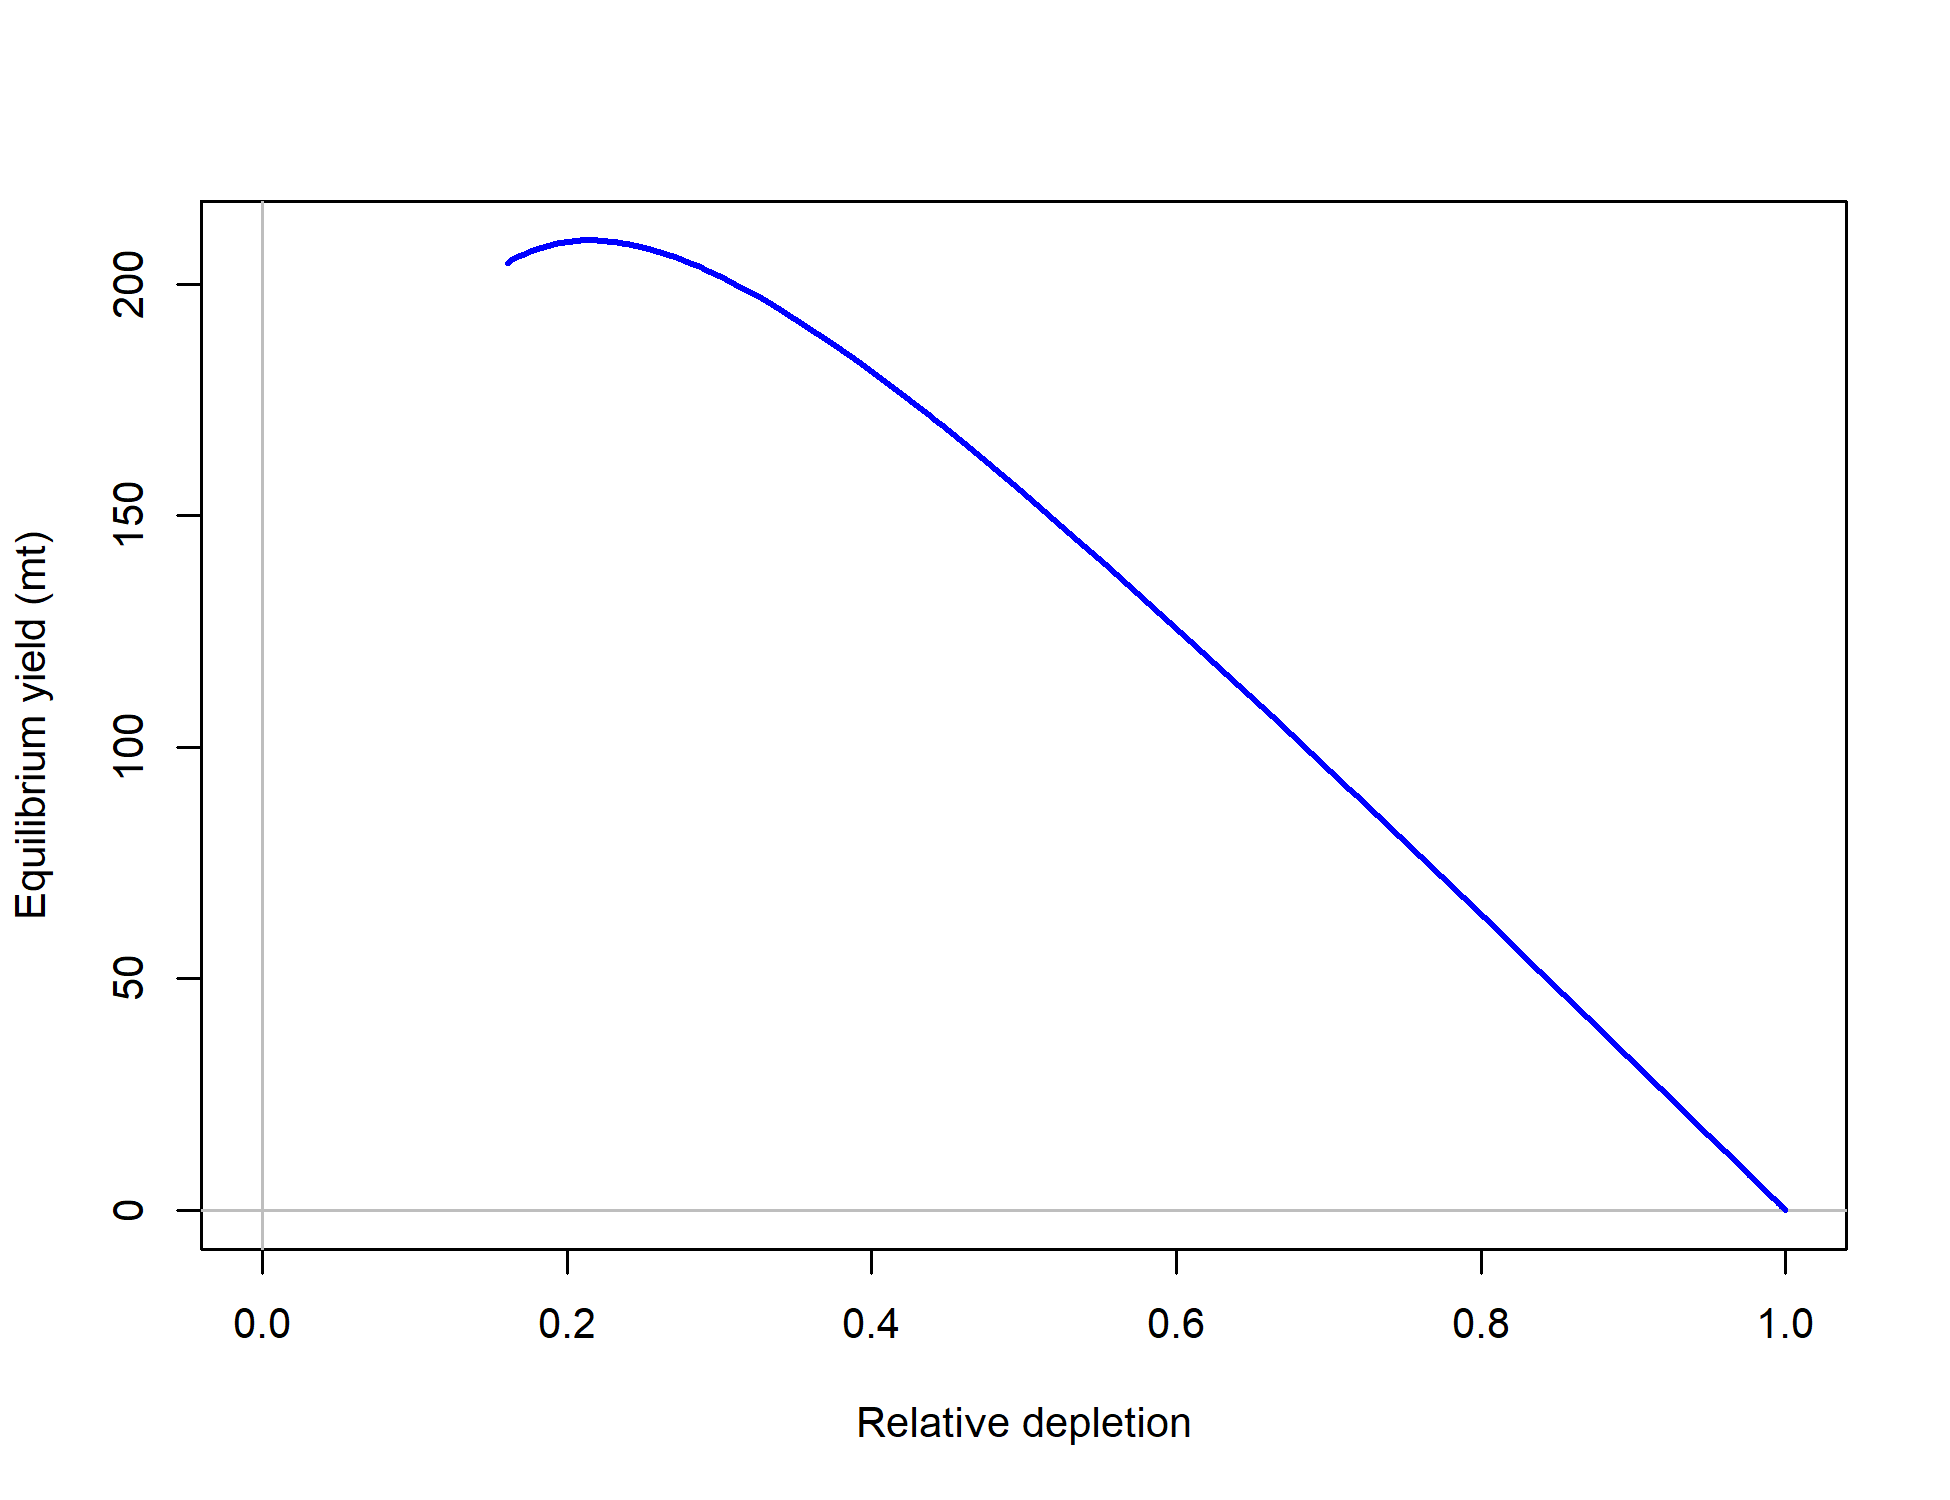
\includegraphics{r4ss/plots_mod1/yield1_yield_curve.png}
\caption{Equilibrium yield curve for the base case model. Values are
based on the 2018 fishery selectivity and with steepness fixed at 0.72.
\label{fig:Yield_all}}
\end{figure}

\FloatBarrier

\newpage

\subsection*{Research and Data Needs}\label{research-and-data-needs}
\addcontentsline{toc}{subsection}{Research and Data Needs}

We recommend the following research be conducted before the next
assessment:

\begin{enumerate}

\item Investigate the structure of complex and contribution of each species to the 
GBYR complex. Investigate possible spatial differences in biological parameters within 
a single species and also between the two species.  Little biological data for south of 
Point Conception or north of Point Arena were available for this assessment and is needed 
to better under biological parameters. 
    \begin{enumerate}
     \item Conduct life history studies
     \item conduct research to identify the proportion of each species in population and in catches
    \end{enumerate}

\item Take a closer look at the Ralston (Ralston et al. 2010) historical catch reconstruction 
for gopher and black-and-yellow rockfishes.  The recreational catch reconstruction for 
gopher rockfish south of Point Conception was an order of magnitude higher than expected 
when extracted for this assessment.  

\item Refine the PISCO survey data and analysis to better identify age-0 fish in each 
month of survey.  Occasional sampling during all months of the year would better help 
identify the length distribution of fish classified as age-0. This is the only recruitment 
index available for gopher and black-and-yellow rockfish. If possible, age data should be 
collected from the PISCO survey to aid in determining the growth of young gopher and 
black-and-yellow rockfish, and larger black-and-yellow rockfish.

\item Refine CCFRP survey index to look at alternative possible model structures, including 
a hierarchical structure and random effects.  Limited time did not allow for these 
explorations during this assessment cycle.  It is also strongly recommended to continue 
the coastwide sampling of the CCFRP program that began in 2017, as well as the collection 
of biological samples for nearshore rockfish species.  The CCFRP survey is the only 
fishery-independent survey available for nearshore rockfish sampling the nearshore rocky 
reef habitats. As of this assessment, only two years of coastwide data are available, 
and the index was limited to the site in central California that have been monitored 
since 2007.

\item Collection of length and age data are recommended for both the commercial and 
recreational fisheries.  Very little age data are available from either fishery for 
gopher rockfish and none for black-and-yellow rockfish.

\item Data collection and coordination across Research Recommendations 1-5 is needed to improve 
the efficacy of data collection and ensure that samples are representative of the 
data sources and the fisheries.  For example, the conditional age-at-length data in 
the dummy fleet represent a number of sampling techniques, areas sampled, and 
selectivities.  Better coordination of research efforts will allow the age data 
to be better utilized by the assessment.  Sampling of the commercial and recreational 
fleets by area in proportion to the length distribution of fish observed will also 
allow the model to better fit selectivity patterns and avoid possible patterns in the 
length and age composition residuals.

\item Investigate possible environmental drivers/co-variates for biological parameters, 
particularly for recruitment.

\item Examine the CFRS angler interview data for the recreational private/rental mode 
to create a "trip" based identifier or catch and effort. This will enable the creation 
of an index of abundance for the private/rental mode as well as investigate if 
selectivity for this mode differs from the party/charter mode.

\item Resolve differences between CalCOM and PacFIN expanded length composition data sets. 


\end{enumerate}

\FloatBarrier

\newpage

\renewcommand{\thefigure}{\arabic{figure}}
\renewcommand{\thetable}{\arabic{table}}

\setcounter{figure}{0} \setcounter{table}{0}

\pagenumbering{arabic}

\section{Introduction}\label{introduction}

\subsection{Basic Information and Life
History}\label{basic-information-and-life-history}

\emph{Population Structure and Complex Assessment Considerations}

There have been a number of analyses conducted on the genetic
differentiation between gopher rockfish and black-and-yellow rockfish.
The studies have yielded a range of results, but have generally
concluded that there is unusually low genetic differentiation between
the two species. The most frequently used measure of genetic analyses to
evaluate evidence for population differentiation is the fixation index
(\(F_{ST}\)), defined as the proportion of the total genetic variation
in one sub-population (subscript S) relative to the total genetic
variation (subscript T) (Hauser and Carvalho
\protect\hyperlink{ref-Hauser2008}{2008}, Waples et al.
\protect\hyperlink{ref-Waples2008}{2008}). Values of \(F_{ST}\) range
from 0 to 1 where a zero value implies the populations are panmictic and
a value closer to one implies the two populations are genetically
independent. Values of \(F_{ST}\) thought to be consistent with
biologically meaningful genetic differentiation and demographic
isolation between populations range from 0.01 to 0.05 (Waples and
Gaggiotti \protect\hyperlink{ref-Waples2006}{2006}). It is also
important to note that \(F_{ST}\) values are dependent on the study's
sample size and it may not necessarily be appropriate to compare them
across studies.

Morphologically, gopher and black-and-yellow rockfishes are almost
indistinct, except for their color variation (Hubbs and Schultz
\protect\hyperlink{ref-Hubbs1933}{1933}). Early efforts to evaluate
whether the two species were genetically distinct began with an allozyme
analysis by Seeb et al. (\protect\hyperlink{ref-Seeb1986}{1986}), which
did not detect genetic differentiation between gopher and
black-and-yellow rockfish. However, as allozymes are proteins that are
often conserved, this early work was not necessarily representative of
genome-wide relationships between the two groups. In a subsequent study
of restriction site polymorphisms, Hunter et al.
(\protect\hyperlink{ref-Hunter1994}{1994}) found slight but significant
differences between species based on restriction fragment length
polymorphisms (RFLP's). Following that study, an analysis of the
mitochondrial control region by Alesandrini and Bernardi
(\protect\hyperlink{ref-Alesandrini1999}{1999}) did not detect
differences between the two species, although mtDNA also has limitations
regarding how results can be extrapolated across the nuclear genome.
Analysis of seven microsatellite loci by Narum et al.
(\protect\hyperlink{ref-Narum2004}{2004}) found an \(F_{ST}\) of 0.049
across the overlapping range of the two species, which provided some
evidence of divergence, although such divergence is relatively low
compared to other species within \emph{Sebastes}. Those authors
characterized their results as suggesting that the two are
``reproductively isolated incipient species.'' Buonaccorsi et al.
(\protect\hyperlink{ref-Buonaccorsi2011}{2011}) found an even lower
\(F_{ST}\) of 0.01 using 25 microsatellite loci, and concluded that
gopher and black-and-yellow rockfish ``have not completed the speciation
process.'' All of these studies are indicative of low levels of genetic
divergence and a high probability of ongoing gene flow between the two
nominal species or incomplete lineage sorting.

Most recently, an analysis of rockfish species assignment using
microhaplotypes by Baetscher
(\protect\hyperlink{ref-Baetscher2019}{2019}) observed mistaken genetic
assignment of a small number of individuals between gopher and
black-and-yellow rockfishes, while no other species among the 54
rockfishes analyzed resulted in mis-assignments. In addition,
comparisons of \(F_{ST}\) values within the study indicated that the
level of genetic differentiation observed between gopher and
black-and-yellow rockfishes is lower (\(F_{ST}\) = 0.015) than that
observed among all other pairwise comparisons of the 54 species in the
\emph{Sebastes} genus that were included in their analysis. Baetscher
(\protect\hyperlink{ref-Baetscher2019}{2019}) characterized the results
as suggestive of the two species representing ``sister species with
evidence of ongoing gene flow,'' noting that a more rigorous evaluation
of the level of genetic distinction between these two species would
benefit from whole-genome sequencing of representatives from each
species group.

In addition to the differences in coloration, the depth distribution and
range differ between the two species. The range of both species extends
from Cape Blanco Oregon to Baja California. Both species are uncommon
north of Fort Bragg, California and black-and-yellow rockfish is
uncommon south of Point Conception, California. However, gopher rockfish
can be found as far south as Punta San Roque on the Baja peninsula.
Gopher rockfish are found in rocky reef habitat from the intertidal to
depths of 264 ft (80 m) with a predominant depth distribution of 30 to
120 ft (9-37 m), while the black-and-yellow rockfish occupies depths
from the intertidal to 120 ft (40 m) and is predominantly observed in
depths shallower than 60 ft (18 m) (Eschmeyer et al.
\protect\hyperlink{ref-Eschmeyer1983}{1983}, Love et al.
\protect\hyperlink{ref-Love2002}{2002}).

Both species are solitary, sedentary, and territorial with home ranges
of 10-12 square meters (Love et al.
\protect\hyperlink{ref-Love2002}{2002}). A large percentage (67-71\%) of
black-and-yellow rockfish returned to the site of capture within two
weeks after translocated within 50 m (Hallacher
\protect\hyperlink{ref-Hallacher1984}{1984}). Lea et al.
(\protect\hyperlink{ref-Lea1999}{1999}) found that gopher rockfish
exhibit minor patterns of movement (\textless{}12.8 km) with all fish
being recaptured on the same reef system where they were tagged.
Matthews (\protect\hyperlink{ref-Matthews1985}{1985}) found that 11.8\%
of tagged and recaptured gopher rockfish, and 25\% of black-and-yellow
rockfish, moved from four low-relief natural reefs to a new high-relief
artificial reef in Monterey Bay. The maximum distance between the
natural and artificial reefs traveled by gopher or black-and-yellow
rockfish was 1.6 km. After only a year, the fish assemblage on the
artificial reef closely resembled that of the nearby natural reefs. The
paper did not address the spatial segregation of gopher and
black-and-yellow rockfish on the new artificial reef.

Larson (\protect\hyperlink{ref-Larson1980}{1980}) conducted a study on
the territoriality and segregation between gopher and black-and-yellow
rockfishes. When one species was removed, the other extended its depth
range to areas where the other previously occupied, indicating
inter-specific competition plays a role in controlling their depth
distributions where both species are present. Of the two species,
black-and-yellow rockfish are socially dominant and aggressive towards
excluding gopher rockfish from shallower waters.

Both species feed at night, with similar diets composed primarily of
crabs and shrimp, supplemented by fish and cephalopods (Larson
\protect\hyperlink{ref-Larson1972}{1972},
\protect\hyperlink{ref-Hallacher1985}{1985}, Love et al.
\protect\hyperlink{ref-Love2002}{2002}). Loury et al.
(\protect\hyperlink{ref-Loury2015}{2015}) found no significant
differences in the diet of gopher rockfish inside and outside the 35
year old Point Lobos Marine Protected Area (MPA). She did find the diet
of gopher rockfish at Año Nuevo (shallower and north of Point Lobos) was
dominated by crabs and dominated by brittle stars at southern, deeper
study locations. Zuercher (\protect\hyperlink{ref-Zuercher2019}{2019})
examined the diets of a suite of nearshore rockfish species including
black-and-yellow and found that they relied on hard-bodied benthic
invertebrates such as Brachyuran crabs, shrimps, other arthropods, and
octopus. The diet of black-and-yellow rockfish remained the same across
sampling years, but they occupied a lower trophic level during the
upwelling season.

\subsection{Early Life History}\label{early-life-history}

Gopher and black-and-yellow rockfish have similar juvenile development.
Both rockfish species are viviparous and release one brood per season
between January and July (Echeverria
\protect\hyperlink{ref-Echeverria1987}{1987}). Larvae are approximately
4 mm in length at birth and have a 1-2 month pelagic stage before
recruiting to the kelp forest canopy, i.e., surface fronds of
\emph{Macrosystis pyrifera} and \emph{Cysteoseira osmundacea} at around
15-21 mm (Anderson \protect\hyperlink{ref-Anderson1983}{1983}, Wilson et
al. \protect\hyperlink{ref-Wilson2008}{2008}). The larvae are
transparent until they reach juvenile stage at 22-23 mm. Differences in
coloration between the two species begin to occur at 25-30 mm and can be
used to identify one species from the other. Gopher rockfish become more
orange and brown, while black-and-yellow rockfish become more black and
yellow.

The juveniles undergo ontogenetic migration down the stalks to deeper
depths, finally settling on rocky reef habitat in their respective adult
depth distribution. Benthic juveniles associate with \emph{Macrosystis}
holdfasts and sporophylls (Anderson
\protect\hyperlink{ref-Anderson1983}{1983}). Juvenile bocaccio and other
fish predate on young of year and other reef dwelling species;
individuals avoid rough surge conditions and predators by hiding in the
rocky bottom during the daylight hours, then returning to more open
water at dusk (Love et al. \protect\hyperlink{ref-Love2002}{2002}).

\subsection{Map}\label{map}

A map showing the scope of the assessment and depicting boundaries at
Cape Mendocino to the north and the U.S./ Mexico border at the south
(Figure \ref{fig:assess_region_map1}). The recreational fishing fleet
was split into two fleets at Point Conception.

\subsection{Ecosystem Considerations}\label{ecosystem-considerations-1}

In this assessment, ecosystem considerations were not explicitly
included in the analysis. This is primarily due to a lack of relevant
data and results of analyses (conducted elsewhere) that could contribute
ecosystem-related quantitative information for the assessment.

\subsection{Fishery Information}\label{fishery-information}

The hook-and-line fishery off California developed in the late 19th
century (Love et al. \protect\hyperlink{ref-Love2002}{2002}). The
rockfish trawl fishery was established in the early 1940s, when the
United States became involved in World War II and wartime shortage of
red meat created an increased demand for other sources of protein (Harry
and Morgan \protect\hyperlink{ref-Harry1961}{1961}, Alverson et al.
\protect\hyperlink{ref-Alverson1964}{1964}).

Gopher and black-and-yellow (referred to from hereon as GBYR when
discussing the complex) rockfish have been a minor component of the
commercial and recreational rockfish fishery since at least the late
1960s (CFIS and RecFIN). The commercial catch histories of the two
species cannot easily be separated (Figure
\ref{fig:Catches_livedeadNS_gby}); from 1916-1936 only black-and-yellow
rockfish were reported in the landings, and an average of 0.04 mt of
black-and-yellow rockfish are reported from 1937-1983. Black-and-yellow
rockfish reappear in the landings in 1984 with 7.2 mt landed
commercially. From 1985-1988 the trend switches and only
black-and-yellow rockfish appear in the commercial landings, with gopher
rockfish averaging 0.1 mt landed, and 0 mt reported in 1987. From 1988
and on, the landings are dominated by gopher rockfish, and both species
are represented in the commercial landings.

The landings from south of Point Conception are minor throughout the
time period, with peaks in the 1950s and 1960s for gopher rockfish.
Black-and-yellow rockfish are rare south of Point Conception and it is
therfore expected that these catches are minimal.

The live fish fishery began in the early 1990s, with the first reported
commercial landings of live gopher rockfish in 1993, and
black-and-yellow rockfish a year later. By 1995 over half (57\%; 39 mt)
of the commercial landings were from the live fish fishery. This
increased quickly over the next few years and has been on average 84\%
of the landed gopher and black-and-yellow rockfish since 2000. The
majority of the landings are from gopher rockfish north of Point
Conception. Landings of live GBYR south of Point Conception were higher
in the late 1990s, (max. 3.2 mt in 1999), and have been averaging 0.4 mt
since 2003.

The ex-vessel value of GBYR increased from less than \$40,000 in 1984
and peaked at \$680,452 in 1996 (source: PacFIN, Figure
\ref{fig:GBY_revenue}). The ex-vessel revenue has been fairly stable at
around \$500,000 a year since 2007. Prior to the live fish fishery in
1994, the average price per pound for either species was around \$2 a
pound. The live fish fishery increased the value of both species to an
average of \$6-\$8 a pound, with maximum reported value of either a
gopher or black-and-yellow rockfish was \$20 a pound in 2003.

The recreational GBYR fishery for California is most prominent north of
Point Conception throughout the entire catch history from 1928 to 1980
(Figure \ref{fig:Exec_catch1}).\\
The sharp increase in the 1980s could be an artifact of the MRFSS
sampling program that began in 1980; however, the more recent
recreational landings also exhibit a cyclical trend of years with high
catches followed by period of decreased recreational landings. The
California Recreational Fisheries Survey (CRFS) era recreational total
mortality represents the most accurate description of the recreational
fleet's catches in terms of area, mode and species (Figure
\ref{fig:CFRS_catches}).

Recreational GBYR catches are dominated by gopher rockfish north of
Point Conception in the private/rental (PR) and party/charter (PC or
CPFV) modes. South of Point Conception gopher rockfish are predominately
caught by the CPFV fleet, with all other modes being insignificant. The
total recreational mortality of black-and-yellow rockfish south of Point
Conception since 2005 is 3 mt, compared to 106 mt north of Point
Conception. The total mortality since 2005 for gopher rockfish is 86 mt
south of Point Conception and 669 mt north of Point Conception.

\subsection{Summary of Management
History}\label{summary-of-management-history}

Prior to the adoption of the Pacific Coast Groundfish Fishery Management
Plan (FMP) in 1982, GBYR were managed through a regulatory process that
included the California Department of Fish and Wildlife (CDFW) along
with either the California State Legislature or the Fish and Game
Commission (FGC) depending on the sector (recreation or commercial) and
fishery. With implementation of the Pacific Coast Groundfish FMP, GBYR
came under the management authority of the Pacific Fishery Management
Council (PFMC), and were managed as part of the \emph{Sebastes} complex.
Because neither species had undergone rigorous stock assessment and did
not compose a large fraction of the landings they were classified and
managed as part of ``Remaining Rockfish'' under the larger heading of
``Other Rockfish'' (PFMC (\protect\hyperlink{ref-PFMC2002}{2002},
\protect\hyperlink{ref-PFMC2004}{2004})).

Since the early 1980s a number of federal regulatory measures have been
used to manage the commercial rockfish fishery including cumulative trip
limits (generally for two- month periods) and seasons. Starting in 1994
the commercial groundfish fishery sector was divided into two
components: limited entry and open access with specific regulations
designed for each component. Other regulatory actions for the general
rockfish categories have included area closures, gear restrictions, and
cumulative bimonthly trip limits set for the four different commercial
sectors - limited entry fixed gear, limited entry trawl, open access
trawl, and open access non-trawl. Harvest guidelines are also used to
regulate the annual harvest for both the recreational and commercial
sectors.

In 2000, changes in the PFMC's rockfish management structure resulted in
the discontinued use of the \emph{Sebastes} complex, and was replaced
with three species groups: nearshore, shelf, and slope rockfishes
(January 4, 2000; 65 FR 221), of which GBYR are included in the
nearshore group. Within the nearshore group, they are included in the
``shallow nearshore rockfish'' component.

During the late 1990s and early 2000s, major changes also occurred in
the way that California managed its nearshore fishery. The Marine Life
Management Act (MLMA), which was passed in 1998 by the California
Legislature and enacted in 1999, required that the FGC adopt an FMP for
nearshore finfish (Wilson-Vandenberg et al.
\protect\hyperlink{ref-Vandenberg2014}{2014}). It also gave authority to
the FGC to regulate commercial and recreational nearshore fisheries
through FMPs and provided broad authority to adopt regulations for the
nearshore fishery during the time prior to adoption of the nearshore
finfish FMP. Within this legislation, the Legislature also included
commercial size limits for ten nearshore species including GBYR (10-inch
minimum size) and a requirement that commercial fishermen landing these
ten nearshore species possess a nearshore permit.

Following adoption of the Nearshore FMP and accompanying regulations by
the FGC in fall of 2002, the FGC adopted regulations in November 2002
which established a set of marine reserves around the Channel Islands in
southern California (which became effective April 2003). The FGC also
adopted a nearshore restricted access program in December 2002 (which
included the establishment of a Deeper Nearshore Permit) to be effective
starting in the 2003 fishing year.

Also, since the enactment of the MLMA, the Council and State in a
coordinated effort developed and adopted various management
specifications to keep harvest within the harvest targets, including
seasonal and area closures (e.g.~the CCAs; a closure of Cordell Banks to
specific fishing), depth restrictions, minimum size limits, and bag
limits to regulate the recreational fishery and license and permit
regulations, finfish trap permits, gear restrictions, seasonal and area
closures (e.g.~the RCAs and CCAs; a closure of Cordell Banks to specific
fishing), depth restrictions, trip limits, and minimum size limits to
regulate the commercial fishery.

The state of California has adopted regulatory measures to manage the
fishery based on the harvest guidelines set forth by the PFMC. The
commercial open access and limited entry fixed gear sectors have
undergone three different spatial management changes since 2000. Since
2005, both have managed the area south of \(40^\circ 10^\prime\) N.
latitude as one area. The open access commercial fishery is managed
based on bimonthly allowable catches, that have ranged from 200 pounds
to 1800 pounds per two months since 2000. From 2005 to 2018, the catch
limits have doubled and are now set at 1200 pounds per two months (for
all months) with March and April remaining closed. The limited entry
fixed gear sector has followed the same pattern as the open access
sector with bi-monthly limits and a doubling of the catch since 2005.
The limited entry trawl fleet is managed on monthly limits on an annual
basis. Since 2011, the limit has been 300 pounds per month for non-IFQ
species. A history of California's commercial regulations from 2000-2018
can be found in
\protect\hyperlink{appendix-a.-californias-commercial-fishery-regulations}{Appendix
A}. A 10-inch total length minimum size limit was implemented in 1999
for both species in the commercial fleet.

Significant regulatory changes in California's recreational sector began
with a change from unlimited number of hooks and lines allowed prior to
2000 to no more than three hooks and one line per angler in 2000. Since
2001, the limit has been no more than two hooks and one line per angler.
There is no size limit in the recreational fishery for gopher or
black-and-yellow rockfish. A nearshore complex sub-bag limit that
included GBYR was in place from 1999 to 2005, but was eliminated
thereafter.

California also began spatial management, including area closures, and
depth restrictions for the recreational fleet in 2000. In general, the
recreational season north of Point Conception extends from April to
December, and south of Point Conception from March to December. In the
area that GBYR are most commonly landed, from Monterey to Morro Bay, the
depth restrictions have been between 30 and 40 fathoms until 2017. In
2017 the depth restrictions were eased by 10 fathoms, opening up fishing
depths along the central California coast that had not been open
consistently since 2002. In both 2017 and 2018, the deepest 10 fathoms
was closed prior to the prescribed season in December due to high
by-catch rates of yelloweye rockfish, one of two rockfish species that
are still overfished. A full history of the recreational regulations
relating to the spatial management of the fleet can be found in
\protect\hyperlink{appendix-b.-californias-recreational-fishery-regulations}{Appendix
B}.

\subsection{Management Performance}\label{management-performance-1}

The contribution of GBYR to the nearshore rockfish OFLs is currently
derived from two sources: 1) forecasts from Key et al.
(\protect\hyperlink{ref-Key2005}{2005}), from Cape Mendocino to Point
Conception, and 2) a Depletion Corrected Average Catch (DCAC (MacCall
\protect\hyperlink{ref-MacCall2009}{2009})) for the area south of Point
Conception. The total mortality of the nearshore rockfish south complex
has been below the ACL in all years (2011-2016). Total mortality
estimates from the NMFS NWFSC are not yet available for 2017-2018. GBYR
total mortality was on average 20\% of the total nearshore rockfish
south total mortality from 2011-2016. The recent GBYR total mortality
contributed approximately 9\% to the nearshore rockfish south OFL, and
GBYR catches have not exceded the GBYR OFLs in recent years. GBYR is a
small component of the nearshore rockfish south complex that includes
twelve other species. A summary of these values as well as other
post-STAR base model summary results can be found in Table
\ref{tab:mnmgt_perform}.

\subsection{Fisheries Off Mexico or
Canada}\label{fisheries-off-mexico-or-canada}

The range of GBYR does not extend north to the Canadian border, and they
are rarely encountered in Oregon and Washington. The southern end of the
gopher rockfish's range extends to Punta San Roque (southern Baja
California) while the southern end of the black-and-yellow rockfish's
range extends to Isla Natividad (central Baja California) (Love et al.
\protect\hyperlink{ref-Love2002}{2002}). However, black-and-yellow
rockfish are rare south of Point Conception, California. This was no
available information on the fishery for GBYR at the time of this
assessment, nor additional details on the abundance or distribution
patterns in Mexican waters.

\section{Assessment}\label{assessment}

\subsection{Data}\label{data}

Data used in the GBYR assessment are summarized in Figure
\ref{fig:data_plot}. Descriptions of the data sources are in the
following sections.

\subsubsection{Commercial Fishery
Landings}\label{commercial-fishery-landings}

\emph{Overview of gopher and black-and-yellow catch histories}

Commercial fishery landings for gopher and black-and-yellow rockfishes
have not been reported consistently by species throughout the available
catch history (Figure \ref{fig:Catches_livedeadNS_gby}). The period from
1916-1935 suggests that only black-and-yellow rockfish were landed in
the commercial fishery, which then switched to predominately gopher
rockfish from 1937-1984. From 1985-1988 the landings data suggest that
only black-and-yellow rockfish were landed and not until 1995 are both
species well-represented in the catches. Pearson et al.
(\protect\hyperlink{ref-Pearson2008}{2008}) noted:

\begin{quote}
The fact that the majority of estimated landings are not based on actual
sampling, combined with the likelihood for misidentification {[}between
gopher and black-and-yellow rockfishes{]}, suggests that our landing
estimates are generally unreliable {[}see Figure 37 in Pearson et al.
(\protect\hyperlink{ref-Pearson2008}{2008}){]}. This is particularly
true for the time interval between 1983 and 1988. Between 1983 and 1988,
market category 962 (group gopher) landings increased sharply while
market category 263 (gopher rockfish) landings declined (not visible in
Figure 37 since the stratum was unsampled and the landings were
converted to unspecified rockfish). Port samples indicated a shift from
gopher rockfish to black-and-yellow rockfish during the same time
interval, suggesting problems with identification. We suggest that if
black-and-yellow landings are combined with gopher landings, the
estimates would be generally reliable for the group.
\end{quote}

There is no way to tease apart the historical catches by species and
even across north and south of Point Conception prior to about 1995.
This precludes the ability to model the catch histories for either
species accurately. Given these constraints, all commercial data were
combined to represent one commercial fleet in the assessment. Additional
details regarding this decision are described below.

The stock assessment of gopher rockfish in 2005 did not excplicitly
include black-and-yellow rockfish landings. A comparison of the
recreational and commercial landings from the 2005 assessment to those
used in this assessment suggest the 2005 assessment may have included
some black-and-yellow rockfish landings (Figure
\ref{fig:Assessment_compare}). The 2005 assessment estimated
recreational landings from 1969-1980 based on a ratio of commercial to
recreational landings, where as this assessment makes use of the
California Catch Reconstruction landings estimates (Ralston et al.
\protect\hyperlink{ref-Ralston2010}{2010}).

\emph{Commercial Landings Data Sources}

The California Catch Reconstruction (Ralston et al.
\protect\hyperlink{ref-Ralston2010}{2010}) contains landings estimates
of commercial landings from 1916-1968 and was queried on 4 April 2019
for GBYR. There were no estimated gopher rockfish landings prior to
1937. Landings in this database are divided into trawl and `non-trawl.'
Since the majority of GBYR are caught in the commercial fixed gear
fisheries, only estimated catch in the `non-trawl' was used. A total of
0.154 mt (3.18\%) were removed from Eureka commercial landings (based on
current proportions of commercial catch from north of Cape Mendocino in
Eureka) since the assessment represents the GBYR stock south of Cape
Mendocino. The majority of GBYR commercial landings (avg. 83\%) are
landed in the Monterey and Morro Bay port complexes.

Contemporary landings were extracted from two data sources, the
California Cooperative Groundfish Survey,
\href{https://calcom.psmfc.org/}{CALCOM}) and the Pacific Fisheries
Information Network (\href{https://pacfin.psmfc.org/}{PacFIN}) landings
databases. Both databases are based on the same data sources (CALCOM
landing receipts), but apply a catch expansion based on different
algorithms. CALCOM collects information including species composition
data (i.e.~the proportion of species landed in a sampling stratum), and
landing receipts (sometimes called ``fish tickets'') that are a record
of pounds landed in a given stratum. Strata in California are defined by
market category, year, quarter, gear group, port complex, and
disposition (live or dead). Although many market categories are named
after actual species, catch in a given market category can consist of
several species. These data form the basis for the ``expanded''
landings, i.e., species composition data collected by port samplers were
used to allocate pounds recorded on landing receipts to species starting
in 1978. Use of the ``Gopher Rockfish'' or the ``Black-and-Yellow
Rockfish'' categories alone to represent actual landings of GBY would
not be accurate.

See Pearson et al. Appendix C
(\protect\hyperlink{ref-Pearson2008}{2008}) for a simple example of the
expansion calculations for the CALCOM database and a description of the
landings in PacFIN can be found in Sampson and Crone
(\protect\hyperlink{ref-Sampson1997}{1997}). Both databases, including
species compositions, and expanded landings estimates are stored at the
Pacific States Marine Fisheries Commission, a central repository of
commercial landings data for the U.S. West Coast. As a note, CALCOM is
the only source for landings from 1969-1980.

Commercial landings from 1981-2018 were queried for a final time from
the CALCOM database on 4 April 2019 and from PacFIN on 3 June 2019.
There are very small differences in commercial landings between CALCOM
and PacFIN from 1981-2018 (Figure \ref{fig:Calcom_vs_Pacfin}). Landings
estimates from PacFIN were used in the assessment (Table
\ref{tab:CommCatches}). Landings were stratified by year, quarter,
live/dead, market category, gear group, port complex, and source of
species composition data (actual port samples, borrowed samples, or
assumed nominal market category). Data from individual quarters were
aggregated at the year level. Fish landed live or dead were combined,
due to changes over time in the reliability of condition information
(Don Pearson, retired NMFS SWFSC, personal communication). From
1916-1968, on average, 74\% of GBYR were landed north of Point
Conception, which rose to 97\% from 1978-2018. Given the smaller
landings south of Point Conception and the similar length composition of
GBYR north and south of Point Conception, no spatial separation was
considered for the commercial fleet.

\subsubsection{Commercial Discards}\label{commercial-discards}

The West Coast Groundfish Observer Program (WCGOP) provides observer
data on discarding across fishery sectors back to 2003. Gopher and
black-and-yellow rockfishes have species-specific depth-stratified
commercial fishery discard mortality rates (Pacific Fishery Managment
Council \protect\hyperlink{ref-PSMFC2018}{2018}). In consultation with
WCGOP staff, the STAT used estimates of total discard mortality from
WCGOP's Groundfish Expanded Mortality Multiyear (GEMM) report as the
best available estimate of discards for GBYR. WCGOP observes between
1-5\% of nearshore fixed gear landings annually south of
\(40^\circ 10^\prime\) N. latitude (coverage rates available
\href{https://www.nwfsc.noaa.gov/research/divisions/fram/observation/data_products/sector_products.cfm\#ob}{here}).
The expanded estimates of total discard weight by species is calculated
as the ratio of the observed discard weight of the individual species
divided by the observed landed weight from PacFIN landing receipts.
WCGOP discard estimates for the nearshore fixed gear fishery take into
account the depth distribution of landings in order to appropriately
apply the depth-stratified discard mortality rates by species (Somers et
al. \protect\hyperlink{ref-Somers2018}{2018}). The discard mortality for
2018 was estimated as an average of the discard mortality from
2013-2017. Discard mortality was estimated from the period prior to
WCGOP discard estimates (1916-2002) based on the average discard
mortality rate from 2004-2017 (2003 was excluded because 2003 discard
mortality was disproportionately higher than all other years) (Table
\ref{tab:CommCatches}).

\subsubsection{Commercial Fishery Length and Age
Data}\label{commercial-fishery-length-and-age-data}

Biological data from the commercial fisheries that caught GBYR were
extracted from CALCOM on 9 May 2019. The CALCOM length composition data
were catch-weighted to ``expanded'' length the raw length composition
data (Table \ref{tab:length_samples_fishery}). The 2005 assessment used
commercial length composition information from CALCOM, but did not
include black-and-yellow rockfish and is not directly comparable. The
2005 assessment used 2 cm length bins from 16-40 cm, where this
assessment uses 1 cm length bins from 4-40 cm. Sex was not available for
the majority (99.5\%) of the commercial length, and the assessment did
not find sexual dimorphism in growth for either species. We aggregated
the commercial length composition among all gears and regions south of
Cape Mendocino.

Discard length compositions from WCGOP (2003-2017) were expanded based
on the discard estimates and were aggregated for all regions south of
Cape Mendocino and across all fixed gear fisheries.

A total of 46 ages were available for gopher rockfish from the
commercial fisheries 2009-2011, 2016, and 2018. Though sparse, the data
were considerd as conditional age-at-length for the commercial fleet,
but not used in the final post-STAR base model.

The input sample sizes for commercial length composition data were
calculated via the Stewart Method for fisheries (Ian Stewart, personal
communication, IPHC, and develped at NWFSC):

\begin{center}

Input effN = $N_{\text{trips}} + 0.138 * N_{\text{fish}}$ if $N_{\text{fish}}/N_{\text{trips}}$ is $<$ 44

Input effN = $7.06 * N_{\text{trips}}$ if $N_{\text{fish}}/N_{\text{trips}}$ is $\geq$ 44

\end{center}

The PacFIN commercial length composition and the expanded catch-weight
length compositions were provided by Andi Stephens (NWFSC) processed
through the
\href{https://github.com/nwfsc-assess/PacFIN.Utilities}{PacFIN
Utilities} package. We compared differences between the catch-weighted
length composition expansions from CALCOM and PacFIN. We were unable to
reconcile the difference between the two data sets. Sample sizes became
more similar if the PacFIN data were restricted to the same market
categories used by CALCOM in the expansion. However, both data sets
apply other filters that we did not have time to explore. For instance,
in the year 2000, 290 more fish were used in the CALCOM expansion than
in PacFIN, but in 2002, 150 more fish were used in the PacFIN expansions
that were not used in CALCOM. Given these caveats, Figure
\ref{fig:Calcom_vs_pacfin_lengths} shows the percent difference in the
expanded length comps within a year. The biggest difference is in length
bin 32 in 2006. However, the same number of fish and samples were used
to expand the 2006 lengths in both databases, indicating there are also
fundamental differences in how the data are treated. Full documentation
is not available for the PacFIN length composition expansion program.
Consequently the STAT chose to use a query that they could completely
understand and selectively develop from the CALCOM database for the base
model, although a sensitivity was conducted using the PacFIN-derived
length composition data.

\subsubsection{Recreational Fishery Landings and
Discards}\label{recreational-fishery-landings-and-discards}

\emph{Historical recreational landings and discards, 1928-1980}

Ralston et al. (\protect\hyperlink{ref-Ralston2010}{2010}) reconstructed
estimates of recreational rockfish landings and discards in California,
1928-1980. Reported landings of total rockfish were allocated to species
based on several sources of species composition data. Estimates of GBYR
landings and discards (combined) from 1928-1979 are available from the
SWFSC. For this assessment, historical recreational catch was stratified
by year and area (north and south of Point Conception). The catches of
GBYR reported in Ralston et al.
(\protect\hyperlink{ref-Ralston2010}{2010}) are higher by an order of
magnitude than expected given the more recent catches of GBYR in the
MRFSS and CRFS eras south of Point Conception (Figure
\ref{fig:Catches_original}). The recreational catches estimated by
Ralston et al. (\protect\hyperlink{ref-Ralston2010}{2010}) were
discussed with the paper's co-authors and also Commercial Passenger
Fishing Vessel (CPFV), i.e., party/charter mode, captains in California.
A consensus was reached that the estimated landings did not accurately
represent the historical GBYR landings and an alternative catch stream
should be developed. One possibility for the inflated catches of GBYR in
southern California is that all nearshore shallow species were combined
and a constant relative fraction between the two was used to assign
catches to each combination of CDFW fishing block and year. The fraction
of GBYR within the nearshore shallow species group was likely
overestimated.

The California Catch Reconstruction applied a linear ramp from 1928-1936
that was not altered in this assessment. From 1937-1979 a linear ramp
was developed from the 1936 estimate to the average recreational landing
from 1980 and 1983 (1981-1982 catches interpolated as described in the
next section) of 4.3 mt. The recreational catches north of Point
Conception were not altered from the original catch reconstruction. The
resulting alternate recreational catch streams are in Table
\ref{tab:Rec_removal} and Figure \ref{fig:Catches_alternate}.

The total difference in the catch streams from Figure
\ref{fig:Catches_original} and Figure \ref{fig:Catches_alternate} is
plotted in Figure \ref{fig:catches_difference}. The differences in the
catches are due to the addition of commercial discards prior to 2004 and
the reduction of the recreational catches south of Point Conception.

\emph{Marine Recreational Fisheries Statistics Survey (MRFSS),
1980-2003}

From 1980-2003, the Marine Recreational Fisheries Statistics Survey
(MRFSS) executed a dockside (angler intercept) sampling program in
Washington, Oregon, and California (see Holliday et al.
(\protect\hyperlink{ref-Holliday1984}{1984}) for a description of
methods). Data from this survey are available from the Recreational
Fisheries Information Network \href{www.recfin.org}{RecFIN}. RecFIN
serves as a repository for recreational fishery data for California,
Oregon, and Washington. Catch estimates for years 1980-2003 were
downloaded on 23 March 2019, and are consistent from 1992-2004 with the
previous assessment (Key et al. \protect\hyperlink{ref-Key2005}{2005})
(Figure \ref{fig:Assessment_compare}).

MRFSS-era recreational removals for California were estimated for two
regions: north and south of Point Conception. No finer-scale estimates
of landings are available for this period. Catches were downloaded in
numbers and weight. Catch in weight is sometimes missing from the
database due to missing average weight estimates. We estimated average
weights based on adjacent strata as needed, although the effect was
relatively minor (7.4 mt over all years for gopher rockfish and 0.6 mt
for black-and-yellow rockfish). Data were not available for the CPFVs in
Northern California from 1980-1982, and we used the average value from
this mode and region from 1983-1987 for these three years. MRFSS
sampling was temporarily suspended from 1990-1992, and we used linear
interpolation to fill the missing years. Sampling of CPFVs in Northern
California was further delayed, and the linear interpolation spans the
period 1990-1995 for this boat mode and region. Landings data for the
shore-based modes (beach/bank, man-made/jetty and shore) were sparse
throughout the MRFSS sampling. All three shore-based modes were combined
by region and linear interpolations were applied missing data in 1981
for the Northern California and 1995, 1996-2001, and 2004 in Southern
California.

Catches from north of Cape Mendocino were removed based on a CRFS-era
average of fraction of recreational landings north of Cape Mendocino by
mode (3.3\% of shore-based, 0.1\% of CPFV, and 0.2\% of private/rental
were removed). From 1980-1989, San Luis Obispo County was sampled as
part of Southern California (personal observation from MRFSS Type 3
sampler examined catch where county is available for 1980-2004). This
assessment separates the recreational fleet at Point Conception.
Recreational landings were re-allocated from southern California from
1980-1992 by fleet based on the average proportion of recreational
landings in northern California from 1996-2004 (after sampling of the
CPFV fleet in northern California resumed). The average proportion
re-allocated from southern to northern California for the CPFV mode was
85\%, 97\% for the private/rental mode, and 81\% for the shore-based
modes. Data were pooled over all years and modes to estimate the
landings re-allocation for the shore-based modes. Total recreational
landings for 1981 and 1982 were 18.8 mt and 18.6 mt, respectively. These
landings were \textgreater{}60 mt lower than any of the neighboring
years. Landings from 1981-1982 were interpolated from the 1980 and 1983
landings.

Onboard sampling of the CPFV fleet began in 1999. A sampler rides along
during a CPFV trip and records the catch from a subset of anglers
onboard the vessel at each fishing location. Effort data are also
recorded, allowing for CPUE calculations at a fine spatial resolution.

\emph{California Recreational Fisheries Survey (CRFS), 2004-2016}

MRFSS was replaced with the California Recreational Fisheries Survey
(CRFS) beginning January 1, 2004. Among other improvements to MRFSS,
CRFS provides higher sampling intensity, finer spatial resolution (6
districts vs.~2 regions), and continued onboard CPFV sampling. Estimates
of catch from 2004-2018 were downloaded from the RecFIN database a final
time on 4 June 2019. We queried and aggregated CRFS data to match the
structure of the MRFSS data, by year, and region (Table
\ref{tab:Rec_removal}). Catches in the shore-based modes are small
compared to the CPFV and private rental modes. All modes are combined,
but separated at Point Conception for two recreational fleets in this
assessment, just as was done for the California Catch Reconstruction and
MRFSS time series.

\emph{Recreational Discards}

Recreational discards were only added to the California Catch
Reconstruction landings, as Ralston et al.
(\protect\hyperlink{ref-Ralston2010}{2010}) did not address discards for
the recreational reconstruction. Recreational removals from the
California Department of Fish and Wildlife MRFSS era (1980-2003)
includes catch type A + B1. Catch type A refers to estimates of catch
based on sampler-examined catch. Catch type B1 includes mainly
angler-reported discard, but also angler-reported retained fish that
were unavailable to the sampler during the interview (e.g., fillets).
The CRFS era removals account for depth-stratified discard mortality
rate and the catch time series includes both retained and discarded
catch (total mortality). We calculated the ratio of dead discards to
total mortality from the CRFS era by region and mode. The region average
across modes was applied to the California Catch Reconstruction as a
constant. The result added 4.68\% annually to recreational removals
north of Point Conception and 4.05\% annually to the removals South of
Point Conception). The final time series of landings and discard
mortality are in Table \ref{tab:Rec_removal}.

\subsubsection{Recreational Fishery Length and Age
Data}\label{recreational-fishery-length-and-age-data}

Recreational length composition samples for California were obtained
from several sources, depending on the time period and boat mode (Table
\ref{tab:length_samples_fishery}). This assessment makes use of a much
longer time series of length composition data, relative to the previous
assessment, as described below. Input sample sizes for recreational
length composition data were based on the number of observed trips, when
available. Other proxies that were used to estimate the number of trips
are described below.

There were no standardized coastwide surveys measuring retained or
discarded fish from the recreational fleet prior to 1980.

\emph{CPFV length composition data, 1959-1978}

The earliest available length data for this assessment were described by
Karpov et al. (\protect\hyperlink{ref-Karpov1995}{1995}), who assembled
a time series (1959-1972) of available California CPFV length data (made
available courtesy of W. Van Buskirk). For GBYR, data from 1959-1961 and
1966 were available north of Point Conception and from 1959-1961 from
south of Pt Conception. A total of 716 (680 north of Point Conception)
unsexed measurements of retained fish (no discards) were included in the
assessment (Table \ref{tab:length_samples_fishery}). Sampling of these
length data did not follow a consistent protocol over time and areas
(data are unweighted), and therefore may not be representative of total
catch. Since the number of trips sampled was not reported by Karpov et
al. (1995), we assume the number of sampled trips is proportional to the
number of measured fish in each year, and estimated the number of trips
using the ratio of fish measured per trip in the MRFSS data (roughly 10
fish per trip).

Collins and Crooke (n.d.) conducted an onboard observer survey of the
CPFV fleet in southern California from 1975-1978. A total of 1,308 GBYR
lengths were available from the study and were assumed to all be from
retained fish. Ally et al. (\protect\hyperlink{ref-Ally1991}{1991})
conducted an onboard observer program of the CPFV fleet from 1985-1987
in southern California. Because MRFSS data were available for this time
period as well and represents multiple recreational modes, the Ally et
al. (\protect\hyperlink{ref-Ally1991}{1991}) length data were not used
in the assessment.

\emph{MRFSS Recreational Length Data, 1980-1989 and 1993-2003}

Unsexed length data of retained fish were collected by MRFSS dockside
samplers and downloaded from the RecFIN website. We identified a subset
of lengths that were converted from weight measurements, and these were
excluded from the final data set (Table
\ref{tab:length_samples_fishery}). The length measurements from Collins
and Crooke (n.d.) from 1975-1978 are assumed to all be from retained
fish. As of 2003, the CDFW Onboard Observer program has taken length
measurements for discarded fish. The retained catch is measured during
the dockside (angler intercept) surveys.

The number of CPFV trips used as initial sample sizes for the MRFSS was
based on the number of CPFV trips was determined from the trip-level
MRFS CPFV database and the number of private boat trips was determined
based on unique combinations of the variables ASSNID ,ID\_CODE,
MODE\_FX, AREA\_X, DIST, INTSITE, HRSF, CNTRBTRS, SUB\_REG, WAVE, YEAR,
and CNTY in the Type 3 (sampler-examined catch) data.

During the recent restructuring of the CRFS data on RecFIN, a ``trip''
identifier was not carried over for all modes, and trip-level sample
sizes could not be extracted from the biological detail table on RecFIN.
A proxy for initial sample sizes for 2004-2018 were developed using the
2015 data for which I had access to raw data files by mode from CDFW. In
more recent years, sampling of the shore-based modes has declined and
were not sampled at all in 2018. Samples sizes were calculated by mode
as the number of port-days (or site-days for shore-based modes) during
bi-weekly intervals (e.g., Jan 1-15, Jan 16-31, etc). The number of
port-days sampled in the bi-weekly intervals was used as the initial
sample size for number of trips to calculate initial input sample sizes
using Ian Stewart's method (described above). All length data were
re-weighted in the assessment model.

\subsubsection{Fishery-Dependent Indices of
Abundance}\label{fishery-dependent-indices-of-abundance}

A summary of all indices in the post-STAR base model can be found in
Table \ref{tab:Index_summary}. Figure \ref{fig:All_index_compare} shows
each index from the pre-STAR base model (before any were modified or
removed from the model) scaled to the mean value of that index to show
them all on the same scale, i.e., the mean of each index in the plot is
1. Figure \ref{fig:All_index_compare_postSTAR} shows the final set of
indices in the post-STAR base model, each scaled to their mean. The
final index values and associated log standard error included in the
assessment can be found in Table \ref{tab:Indices}.

\textbf{MRFSS Dockside CPFV Index}

From 1980 to 2003 the MRFSS program conducted dockside intercept surveys
of recreational fishing fleet. The program was temporarily suspended
from 1990-1992 due to lack of funding. For purposes of this assessment,
the MRFSS time series was truncated at 1998 due to sampling overlap with
the onboard observer program (i.e., the same observer samples the catch
while onboard the vessel and also conducts the dockside intercept survey
for the same vessel). Each entry in the RecFIN Type 3 database
corresponds to a single fish examined by a sampler at a particular
survey site. Since only a subset of the catch may be sampled, each
record also identifies the total number of that species possessed by the
group of anglers being interviewed. The number of anglers and the hours
fished are also recorded. The data, as they exist in RecFIN, do not
indicate which records belong to the same boat trip. A description of
the algorithms and process used to aggregate the RecFIN records to the
trip level is outlined Supplemental Materials (``Identifying Trips in
RecFIN'').

Initial trip filters included eliminating trips targeting species caught
near the surface waters for all or part of the trip, including trips
with catch of bluefin tuna, yellowfin tuna, skipjack, and albacore.
Trips occuring in bays, e.g., San Francisco Bay, were also excluded.

The following filtering steps were applied to gopher rockfish, as well
as the sum of the two species to represent GBYR. No filtering or indices
were developed for black-and-yellow rockfish alone due to the sparseness
in the data. In the raw data, unfiltered data, black-and-yellow rockfish
only occurred in 48 trips that did not also observe gopher rockfish.
There were an additional 65 trips that encountered both species. There
was little difference between indices developed for gopher-only and the
GBYR complex for both north and south of Point Conception (Figure
\ref{fig:MRFSS_index_compare}). The descriptions of the filtering and
data below represent those for the GBYR complex.

The species composition of catch in California varies greatly with
latitude. Therefore, Stephens-MacCall filtering was applied
independently for north and south of Point Conception. Separate indices
were also developed to represent two recreational fleets in the model.
Since recreational fishing trips target a wide variety of species,
standardization of the catch rates requires selecting trips that are
likely to have fished in habitats containing GBYR. The Stephens-MacCall
(\protect\hyperlink{ref-Stephens2004}{2004}) filtering approach was used
to identify trips with a high probability of catching GBYR, based on the
species composition of the catch in a given trip. Prior to applying the
Stephens-MacCall filter, we identified potentially informative predictor
species, i.e., species with sufficient sample sizes and temporal
coverage (at least 30 positive trips total) to inform the binomial
model. Coefficients from the Stephens-MacCall analysis (a binomial GLM)
are positive for species which co-occur with GBYR, and negative for
species that are not caught with GBYR. Each of these filtering steps and
the resulting number of trips remaining in the sampling frame are
provided in Table \ref{tab:Fleet10_11_Filter}.

\emph{MRFSS Filtering and Index Standardization for North of Point
Conception.} Prior to the Stephens-MacCall filter, a total of 2,788
trips were retained for the analysis. As expected, positive indicators
of GBYR trips include several species of nearshore rockfish, treefish,
kelp rockfish, and blue rockfish, and the strongest counter-indicator
was striped bass (Figure \ref{fig:Fleet10_SM_filter}). While the filter
is useful in identifying co-occurring or non-occurring species assuming
all effort was exerted in pursuit of a single target, the targeting of
more than one target species can result in co-occurrence of species in
the catch that do not truly co-occur in terms of habitat associations
informative for an index of abundance. Stephens and MacCall (Stephens
and MacCall \protect\hyperlink{ref-Stephens2004}{2004}) recommended
including all trips above a threshold where the false negatives and
false positives are equally balanced. However, this does not have any
biological relevance and for this data set, we assume that if a GBYR was
landed, the anglers had to have fished in appropriate habitat,
especially given how territorial GBYR and both species are strongly
associated with rocky habitat.

Two levels of possible filtering were applied using the Stephens-MacCall
filter (Table \ref{tab:Fleet10_11_Filter}). The Stephens-MacCall
filtering method identified the probability of occurrence (in this case
0.4) at which the rate of ``false positives'' equals ``false
negatives.'' The trips selected using this criteria were compared to an
alternative method including all the ``false positive'' trips,
regardless of the probability of encountering GBYR (Table
\ref{tab:Fleet10_contingency} and Figure
\ref{fig:MRFSS_index_N_SM_falsepos}). This assumes that if GBYR were
caught, the anglers must have fished in appropriate habitat during the
trip. The catch included in this index is ``sampler-examined'' and the
samplers are well trained in species identification. The last filter
applied was to exclude years after 1999 due to a number of regulation
changes, and years in which there were less than 20 observed trips. The
final index is represented by 544 trips, 220 of which encountered GBYR.

Due to the large number of zeros in the data, we modeled catch per
angler hour (CPUE; number of fish per angler hour) using maximum
likelihood and Bayesian negative binomial regression. Models
incorporating temporal (year, 2-month waves) and geographic (region and
area\_x) factors were evaluated. Counties were grouped into three
regions, north of Sonoma county, Sonoma county through Santa Cruz
county, and San Luis Obispo county. Based on AIC values from maximum
likelihood fits (Table \ref{tab:Fleet10_AIC}), a main effects model
including all factors (year, region, area\_x, and 2-month waves) was fit
in the ``rstanarm'' R package (version 2.18.2). Diagnostic checks of the
Bayesian model fit (Neff, Rhat, and Monte Carlo standard error values)
were all reasonable. Predicted means by stratum (Year) were strongly
correlated with observed means, suggesting a reasonable fit to the data
(Figure \ref{fig:Fleet10_MLE_stan}). The NB model generated data sets
with roughly 50-70\% zeros, compared to the observed 60\% (Figure
\ref{fig:Fleet10_prop_zero_STAN}).

The index represents the years 1984-1989, 1995, 1996 and 1999. There is
not a lot of contrast in the index, except for a small increase in 1986.
The final index values and associated log standard error included in the
assessment can be found in Table \ref{tab:Indices}.

\emph{MRFSS Filtering and Index Standardization for South of Point
Conception.}\\
Note, the MRFSS index for south of Point Conception was not used in the
post-STAR base model.

Prior to the Stephens-MacCall filter, a total of 7,334 trips were
available for the analysis. As expected, positive indicators of GBYR
trips included several nearshore species, e.g., kelp rockfish, treefish,
and black croaker, while the strongest counter-indicator was opaleye
(Figure \ref{fig:Fleet11_SM_filter}). While the filter is useful in
identifying co-occurring or non-occurring species assuming all effort
was exerted in pursuit of a single target, the targeting of more than
one target species can result in co-occurrence of species in the catch
that do not truly co-occur in terms of habitat associations informative
for an index of abundance. For consistency with the methods used north
of Point Conception (Table \ref{tab:Fleet10_11_Filter}) the index
includes the trips identified as ``false positives'' from the
Stephens-MacCall filtering that had a lower threshold level of 0.22
(Table \ref{tab:Fleet11_contingency}). The last filter applied was to
exclude years after 1999 due to a number of regulation changes, and
years in which there were less than 20 observed trips. The final index
is represented by 475 trips, 342 of which encountered GBYR.

Catch per angler hour (CPUE; number of fish per angler hour) was modeled
using the delta-GLM approach (Lo et al.
\protect\hyperlink{ref-Lo1992}{1992}, Stefánsson
\protect\hyperlink{ref-Stefansson1996}{1996}). A negative binomial model
was explored, but the proportion of zeroes was not well estimated in the
negative binomial models. This is likely due to the facts that MRFSS
sampling effort was higher south of Point Conception, and GBYR are also
rare south of Point Conception, both leading to a higher proportion of
zeroes in the trip data than for north of Point Conception.

Model selection using Akaike Information Criterion (AIC) supported
inclusion of year, region, area\_x, and 2-month waves (Table
\ref{tab:Fleet11_AIC}). Counties were grouped into three regions, Santa
Barbara to Ventura counties, Los Angeles and Orange counties, and San
Diego county for both the positive observation model and the binomial
model. Area\_x is a measure of distance from shore, a categorical
variable indicating whether most of the fishing occurred inside or
outside three nautical miles from shore.

The resulting index for south of Point Conception represents different
years than the index for north of Point Conception (Table
\ref{tab:Indices}). The index starts in 1980 with continuous data
through 1986, and three additional years in 1996, 1998 and 1999. The
index increases through 1983 and a marked decrease to 1986. The index
for the three years in the 1990s does not exhibit any significant trend.

\textbf{CPFV Onboard Observer Surveys}

Onboard observer survey data were available from three sources for this
assessment, 1) a CDFW survey in central California from 1987-1998
(referred to as the Deb Wilson-Vandenberg onboard observer survey,
(Reilly et al. \protect\hyperlink{ref-Reilly1998}{1998})) the CDFW CPFV
onboard observer survey from 1999-2018, and 3) a Cal Poly survey from
2003-2018. During an onboard observer trip the sampler rides along on
the CPFV and records location-specific catch and discard information to
the species level for a subset of anglers onboard the vessel. The subset
of observed anglers is usually a maximum of 15 people the observed
anglers change during each fishing stop. The catch cannot be linked to
an individual, but rather to a specific fishing location. The sampler
also records the starting and ending time, number of anglers observed,
starting and ending depth, and measures discarded fish. The fine-scale
catch and effort data allow us to better filter the data for indices to
fishing stops within suitable habitat for the target species.

The state of California implemented a statewide onboard observer
sampling program in 1999 (Monk et al.
\protect\hyperlink{ref-Monk2014}{2014}). California Polytechnic State
University (Cal Poly) has conducted an independent onboard sampling
program as of 2003 for boats in Port San Luis and Morro Bay, and follows
the protocols established in Reilly et al.
(\protect\hyperlink{ref-Reilly1998}{1998}). Cal Poly has modified
protocols reflect sampling changes that CDFW has also adopted, e.g.,
observing fish as they are encountered instead of at the level of a
fisher's bag. Therefore, the Cal Poly data area incorporated in the same
index as the CDFW data from 1999-2018. The only difference is that Cal
Poly measures the length of both retained and discarded fish.

We generated separate relative indices of abundance in for the 1987-1999
and 2000-2018 data sets due to the number of regulation changes
occurring throughout the time period (see
\protect\hyperlink{appendix-b.-californias-recreational-fishery-regulations}{Appendix
B}). Separate indices were also developed for north and south of Point
Conception.

\emph{Deb Wilson-Vandenberg Onboard Observer Index Filtering and
Standardization.} A large effort was made by the SWFSC to recover data
from the original data sheets for this survey and developed into a
relational database (Monk et al.
\protect\hyperlink{ref-Monk2016}{2016}). The specific fishing locations
at each fishing stop were recorded at a finer scale than the catch data
for this survey. We aggregated the relevant location information (time
and number of observed anglers) to match the available catch
information. Between April 1987 and July 1992 the number of observed
anglers was not recorded for each fishing stop, but the number of
anglers aboard the vessel is available. We imputed the number of
observed anglers using the number of anglers aboard the vessel and the
number of observed anglers at each fishing stop from the August
1992-December 1998 data (see Supplemental materials for details). In
1987, trips were only observed in Monterey, CA and were therefore
excluded from the analysis. The years 1990 and 1991 were also removed
for low sample sizes. Final data filters included removing reefs that
never encountered GBYR, drifts that had fishing times outside 95\% of
the data, and fishing stops with depths \textless{}9 m and
\textgreater{}69m (Table \ref{tab:Fleet5_Filter}). The final data set
contained 2,411 fishing stops, with 1,096 of those encountering GBYR
(Figure \ref{fig:DebWV_sites}).

The index was fit using a delta-GLM model, with a lognormal model (AIC:
1,088) selected over a gamma model (AIC: 1,143) for the positive
encounters. Covariates considered in the full model included year,
depth, and month (Table \ref{tab:Fleet5_AIC}). The model selected by AIC
for both the lognormal and binomial components of the delta-GLM included
year, depth and reef. Depth was included in 10 m depth bins and eight
reefs were select in the final model. The final index did not indicate
an increasing trend that was seen in the 2005 gopher rockfish assessment
using the same data set (Figure \ref{fig:DebWV_index_compare}). A number
of reasons include that finer-scale location data was keypunched in 2012
for this survey, the index in this assessment includes black-and-yellow
rockfish, and different filters were applied to the data. However, the
the same peaks and decreases in the two indices are present.

\emph{CDFW and Cal Poly Onboard Observer Index Filtering and
Standardization} As described above the CDFW and Cal Poly onboard
observer programs are identical in that the same protocols are followed.
The only difference is that Cal Poly measures both retained and
discarded fish from the observed anglers and CDFW measures only
discarded fish from the observed anglers. CDFW measures retained fish as
part of the angler interview at the bag and trip level. Cal Poly has
also begun collecting otoliths during the onboard observer trips, which
are used as conditional age-at-length data the recreational fishery
north of Point Conception in this assessment.

A number of filters are applied to these data. All of the Cal Poly data
have been through a QA/QC process once key-punched, whereas a number of
errors remain in the data from CDFW. Data sheets from CDFW are no longer
available prior to 2012 and staff constraints have also prevented a
quality control review of the data.

Each drift was assigned to a reef (hard bottom). Hard bottom was
extracted from the
\href{http://seafloor.otterlabs.org/index.html}{California Seafloor
Mapping Project}, with bathymetric data from state waters available at a
2 m resolution. Reefs were developed based on a number of factors
described in the supplemental material (``Reef Delineation''). Reefs
outside the state boundary not included in the high resolution mappin
project were mapped using other data sources.

Initial filters were applied to the entire data set, north and south of
Point Conception combined. After an initial clean-up of the data, 67,850
drifts remained, with GBYR present in 9,317 (Table
\ref{tab:Fleet6_7_Filter}). This was reduced to 25,427 drifts with GBYR
present in 7,250 drifts after filtering the data to remove potential
outliers in the time fished and observed anglers, limiting the data to
reefs that observed GBYR and were sampled in at least 2/3 of all years,
and to drifts with starting locations within 1,000 m of a reef.

Recreational fishing trips north and south of Point Conception can be
fundamentally different due to differences in habitat structure, target
species, and weather.

\emph{Filtering and Index Standardization for north of Point Conception}
The number of drifts remaining before region specific filtering was
13,792, with 6,036 drifts encountering GBYR (Table
\ref{tab:Fleet6_7_Filter}).\\
Because GBYR are strongly associated with hard bottom habitat, the
distance from a reef at the start of a drift was re-examined for drifts
encountering GBYR. The maximum distance was 872 m, but the 97\% quantile
dropped to 42 m and was chosen as a reasonable cutoff value, and only
resulted in a reduction of 182 drifts that encountered gopher rockfish.
The final data were filtered to ensure all selected reefs were sampled
in at least 2/3 of all years, leaving 12,965 drifts for the final index,
5,796 of which encountered GBYR (Figure
\ref{fig:Onboard_observer_north_sites}).

The index of abundance was modeled with a delta-GLM modeling approach,
with year, month, 10 m depth bins from 10-59 m, and 12 reefs as possible
covariates. A lognormal model (AIC: 12,185) was selected over a gamma
(AIC: 12,520) for the positive observations using AIC (Table
\ref{tab:Fleet6_AIC}). The full model was selected by AIC for the
lognormal and binomial components of the delta-GLM. The index indicates
a relatively stable trend from 2001-2009 and a steady decrease from
2010-2013. The relative index of abundance has increased since 2014.

\emph{Filtering and Index Standardization for south of Point Conception}

Note, the CPFV onboard index for south of Point Conception was not used
in the final post-STAR base model.

The bathymetric data is not available at as fine-scale resolution for
the Southern California Bight and more of the trips and drifts target
mid-water species, including mid-water rockfish (Table
\ref{tab:Fleet6_7_Filter}). Therefore, instead of using distance to reef
as a filter, we filtered the data to drifts that encountered 20\% or
more groundfish. This resulted in the total number of drifts decreasing
from 11,635 to 5,495, but only decreased the number of drifts
encountering GBYR from 1,277 to 1,171. A final check was made to ensure
all reefs were sampled in at least 2/3 of all years, leaving 5,440 drift
for the final index, of which 1,132 encountered GBYR (Figure
\ref{fig:Onboard_observer_south_sites}).

The index of abundance was modeled with a delta-GLM modeling approach,
with year, month, 10 m depth bins from 10-59 m, and four reefs as
possible covariates. A lognormal model (AIC: 162) was selected over a
gamma (AIC: 277) for the positive observations using AIC (Table
\ref{tab:Fleet7_AIC}). A model with year, depth and reef was selected by
AIC for both the lognormal and binomial components of the delta-GLM. The
index indicates a relatively stable trend from 2001-2004 and a steady
increase from 2005-2017.

\subsubsection{Fishery-Dependent Indices: Available Length and Age
Data}\label{fishery-dependent-indices-available-length-and-age-data}

Length data associated with the MRFSS dockside CPFV survey and the
current onboard observer surveys conducted by CDFW are incorporated into
the biological data pulled from the respective data sources, MRFSS and
CRFS. The additional length data are not incorporated as separate length
composition data as they represent the same portion of the population
sampled by the CDFW onboard observer program.

Cal Poly collected otoliths from the onboard observer program starting
in 2017 as part of a special study to correlate fish length before and
after the fish was filleted by the deckhands onboard the CPFV vessels.
All fish collected in 2017 only had associated post-fillet lengths and
were not used in the assessment since the study has not been finalized
nor has the method been endorsed by the SSC. A subset of fish form the
2018 collection included both pre- and post-fillet length and were used
in the assessment as conditional age-at-length data associated with the
recreational fleet north of Point Conception.

Length composition from Deb Wilson-Vandenberg's onboard observer survey
are included in the assessment. This program measured both retained and
discarded fish, and represent the portion of the population sampled with
the spatial extent of the index. This onboard observer program continued
during the period from 1990-1992 when MRFSS was on hiatus.

\subsubsection{Fishery-Independent Data
Sources}\label{fishery-independent-data-sources}

The PISCO survey data have previously been used in one stock assessment
(cabezon) and the CCFRP data have not previously been used in stock
assessments as an index of abundance.

\textbf{California Collaborative Fisheries Research Project}

The California Collaborative Fisheries Research Project,
\href{https://www.mlml.calstate.edu/ccfrp/}{CCFRP}, is a
fishery-independent hook-and-line survey designed to monitor nearshore
fish populations at a series of sampling locations both inside and
adjacent to MPAs along the central California coast (Wendt and Starr
\protect\hyperlink{ref-Wendt2009}{2009}, Starr et al.
\protect\hyperlink{ref-Starr2015}{2015}). The CCFRP survey began in 2007
and was originally designed as a statewide program in collaboration with
NMFS scientists and fishermen. From 2007-2016 the CCFRP project was
focused on the central California coast, and has monitored four MPAs
consistently since then (Figure \ref{fig:CCFRP_sites}). In 2017, the
program was expanded coastwide within California. The index of abundance
was developed from the four MPAs sampled consistently (Año Nuevo and
Point Lobos by Moss Landing Marine Labs; Point Buchon and Piedras
Blancas by Cal Poly).

The survey design for CCFRP consists a number 500 x 500 m cells both
within and outside each MPA. On any given survey day site cells are
randomly selected within a stratum (MPA and/or reference cells). CPFVs
are chartered for the survey and the fishing captain is allowed to
search within the cell for a fishing location. During a sampling event,
each cell is fished for a total of 30-45 minutes by volunteer anglers.
Each fish encountered is recorded, measured, and can be linked back to a
particular angler, and released (or descended to depth). Starting in
2017, a subset of fish have been retained to collect otoliths and fin
clips that provide needed biological information for nearshore species.
For the index of abundance, CPUE was modeled at the level of the drift,
similar to the fishery-dependent onboard observer survey described
above.

The CCFRP data are quality controlled at the time they are key punched
and little filtering was needed for the index (Table
\ref{tab:Fleet9_Filter}). Cells not consistently sampled over time were
excluded as well as cells that never encountered GBYR. CCFRP samples
shallower depths to avoid barotrauma-induced mortality. The index was
constrained to 5-39m in 5 m depth bins. The final index included 4,920
drifts, 3,848 of which encountered GBYR.

We modeled catch per angler hour (CPUE; number of fish per angler hour)
using maximum likelihood and Bayesian negative binomial regression. The
proportion of zeroes in this data was relatively small (22\%), and if
overdispersion were not present, the regression would innately become
Poisson. Models incorporating temporal (year, month) and geographic (MPA
site and MPA vs Reference cells) factors were evaluated. Based on AIC
values from maximum likelihood fits (Table \ref{tab:Fleet9_AIC}), a main
effects model including all factors (year, month, site and MPA/REF) was
fit in the ``rstanarm'' R package (version 2.18.2). Diagnostic checks of
the Bayesian model fit (Neff, Rhat, and Monte Carlo standard error
values) were all reasonable. Predicted means by stratum (Year) were
strongly correlated with observed means, suggesting a reasonable fit to
the data (Figure \ref{fig:Fleet9_MLE_stan}). The NB model generated data
sets with roughly 18-22\% zeros, compared to the observed 22\% (Figure
\ref{fig:Fleet9_prop_zero_STAN}).

The CCFRP index of abundance closely matches the trend observed in the
CDFW/Cal Poly onboard observer index from 2009-2018 (Figure
\ref{fig:All_index_compare}). The index decreases from 2009 to 2013, and
then exhibits the same increase through 2018. When both indices are
standardized to their means, the values for 2013 and 2018 are the same.

\emph{CCFRP Length Measurements and Available Ages}

The CCFRP program measures every fish encountered to the nearest half
centimeter. A total of 22,470 GBYR were measured by CCFRP from
2007-2018, of which only 212 were black-and-yellow rockfish. The length
distributions for each of the four MPAs used in the index for this
assessment show slight differences in the peak length (Figure
\ref{CCFRP_lengths_by_site}). Año Nuevo is the most northern site and
Point Buchon the most southern.

Conditional age-at-length data were also incorporated into the
assessment from the CCFRP program, including two master's theses that
are products of the CCFRP. Erin Loury (Loury
\protect\hyperlink{ref-Loury2011}{2011}) collected gopher rockfish
otoliths as part of her thesis work from 2007-2009 that included
specimens from both inside and outside the MPAs. Natasha Meyers-Cherry
(Meyers-Cherry \protect\hyperlink{ref-MeyersCherry2014}{2014}) conducted
another thesis focused on the life history of gopher rockfish and
collected otoliths from 2011-2012, also both inside and outside the
MPAs. Both MLML and Cal Poly began routinely collecting otoliths from a
select number of fish in 2017 as part of the CCFRP program. Also
included in the conditional age-at-length data for this fleet are
otoliths collected in 2018 by the University of California Davis Bodega
Marine Lab CCFRP program.

\textbf{Partnership for Interdisciplinary Studies of Coastal Oceans}

The Partnership for Interdisciplinary Studies of Coastal Oceans,
\href{http://www.piscoweb.org/kelp-forest-study}{PISCO-UCSC}, conducts a
number of surveys to monitor the kelp forests, one of which is a kelp
forest fish survey. PISCO has monitored fish population in the 0-20 m
depth range as part of the Marine Life Protection Act (MLPA) since 1998.
Paired sites inside and outside MPAs are surveyed to monitor the
long-term dynamics of the kelp forest ecosystem and provide insight into
the effect of MPAs on kelp forest species. PISCO conducts the fish
surveys from late July through September. At each site, benthic,
midwater, and canopy scuba transects are conducted at 5, 10, 15, and 20
m depth. All divers are trained in species identification. Along each 30
m transect, divers enumerate all identifiable non-cryptic fish, and
measure total length to the nearest centimeter. PISCO surveys are
conducted by the University of California Santa Cruz (UCSC) in central
California and through the University of California Santa Barbara in
southern California. All PISCO data were provided by Dan Malone (UCSC).

The majority of filtering for the PISCO data set was to determine which
sites to retain for the final index (Table \ref{tab:Fleet8_Filter}).
After initial filtering the data for GBYR in southern California were
too sparse to be considered for the index of abundance. Gopher and
black-and-yellow rockfish were also rarely observed in the midwater and
canopy transects, and therefore the index is based only on the benthic
transects. Only sites sampled consistently throughout the time period
2001-2018 were kept for the index. Multiple transects can be conducted
along the same line within a sampling event. All transects within a site
were combined and effort was modeled as the number of transects
represented in the number of fish observed. The final index included
3,231 transects, of which 1,729 observed GBYR (Figure
\ref{fig:PISCO_sites}).

Three indices are described below. The pre-STAR base model includes a
single index of abundance for the PISCO survey. During the STAR panel
the decision was made to include two separate indices of abundance and
selectivities for the PISCO data. The PISCO data include information on
age-0 recruitment and also older fish. The PISCO age-0 recruitment index
includes fish that are 6 cm or smaller, and the PISCO index for larger
fish includes fish 15 cm and larger. There is uncertainty in the age of
fish in the 7-14 cm range due to the timing of sampling, growth, and the
timing of ages, i.e., all fish turn one on Jan 1 in the SS assessment
model. Additionally, fish in the 7-14 cm are also not well sampled by
the survey.

For all three iterations of the index we modeled number of fish observed
per transect(s) using maximum likelihood and Bayesian regression. The
index containing all data and the index for larger fish (15+ cm) only
were modeled as negative binomial, whereas the data for the age-0 (for
which the 4-6 cm fish serve as a proxy) index were sparse and modeled as
binomial. Models incorporating temporal (year, month) and geographic
(site and zone) factors were evaluated. The zone is a factor indicating
the depth stratification at a site, i.e., 5 m, 10 m, 15 m, or 20 m
targeted bottom depth.

\emph{Index based on all of the PISCO data (used in the pre-STAR base
model).}\\
Based on AIC values from maximum likelihood fits (Table
\ref{tab:Fleet8_AIC}), a main effects model including all factors (year,
month, site and zone) was fit in the ``rstanarm'' R package (version
2.18.2). Diagnostic checks of the Bayesian model fit (Neff, Rhat, and
Monte Carlo standard error values) were all reasonable. Predicted means
by stratum (Year) were strongly correlated with observed means,
suggesting a reasonable fit to the data (Figure
\ref{fig:Fleet8_MLE_stan}). The NB model generated data sets with
roughly 16-25\% zeros, compared to the observed 23\% (Figure
\ref{fig:Fleet8_prop_zero_STAN}).

The final index decreases from 2001 to the late 2000s, with lower
estimates of relative abundance from 2005-2010. From 2010 to 2015, the
index increases and peaks in 2015, before the decreasing trends from
2016-2018. The trend observed in this index is counter to that observed
in the onboard observer and CCFRP indices for north of Point Conception
(Figure \ref{fig:All_index_compare}). The PISCO survey is sampling
different habitat types than the other two surveys, and covers much
shallower depths. It's possible that the PISCO index captures
recruitment pulses, but because this index includes both
young-of-the-year and adult fish, the trend may be captured in the
model.

\emph{PISCO index based on fish 15 cm and larger (used in the post-STAR
base model).}\\
The same filtered dataset was used for the index for fish 15 cm and
larger as for the PISCO index that included all fish. Based on AIC
values from maximum likelihood fits (Table \ref{tab:Fleet8large_AIC}), a
main effects model including all factors (year, month, site and zone)
was fit in the ``rstanarm'' R package (version 2.18.2). Diagnostic
checks of the Bayesian model fit (Neff, Rhat, and Monte Carlo standard
error values) were all reasonable. Predicted means by stratum (Year)
were strongly correlated with observed means, suggesting a reasonable
fit to the data (Figure \ref{fig:Fleet8large_MLE_stan}). The NB model
generated data sets with roughly 20-30\% zeros, compared to the observed
25\% (Figure \ref{fig:Fleet8large_prop_zero_STAN}).

\emph{PISCO recruitment index based on fish 6 cm and smaller (used in
the post-STAR base model).}\\
The same filtered dataset was used for the index for fish 15 cm and
larger as for the PISCO index that included all fish. There was no
consistent pattern in the presence of age-0 fish to exclude any sites or
zones. All years were included in the final index, even if sample sizes
were small. Age-0 fish were present in 14\% of all transects. A negative
binomial model was not well fit to the data so a binomial
(presence/absence) model was selected for the recruitment index. Based
on AIC values for maximum likelihood fits (Table
\ref{tab:Fleet8age0_AIC}), a main effects model including year, month,
and zone was fit in the ``rstanarm'' R package (version 2.18.2). The
resulting index has large standard errors for years with sparse data,
including 2004-2008 and 2012-2013. A recruitment signal is present in
the index in a number of years, including 2001-2003, 2010, and
2014-2017.

\emph{PISCO Length Measurements}

All but one GBYR observed by PISCO divers was measured (N = 11,965).
Divers measure fish to the nearest centimeter, and are trained to
measure fish underwater and be aware of possible biases, e.g., ambient
light, body color, visibility, and body shape. Both juvenile and adult
GBYR were observed in the PISCO kelp forest fish survey data (Figure
\ref{fig:PISCO_lengths}). Of note is the similarity in length
distributions both between the species and for the two species combined
across sites. Fish in the 10-17 cm size range (approximately) are rarely
observed in this survey. There is significant post-settlement mortality
for both species, which is thought to be due to density-dependent
predation (Johnson \protect\hyperlink{ref-Johnson2006}{2006},
\protect\hyperlink{ref-Johnson2007}{2007}). Secondly, both species can
be cryptic and observed at higher frequency by divers at night than
during the day (Mark Carr, PISCO-UCSC, personal communication).

\subsubsection{Biological Parameters and
Data}\label{biological-parameters-and-data}

Neither gopher nor black-and-yellow rockfish have forked tails,
therefore total length and fork length are equal. All of the data
provided for this assessment were either in fork length or total length.

\textbf{Length and Age Compositions}

Length compositions were provided from the following sources:

\begin{itemize}[noitemsep,nolistsep,topsep=0pt]
  \item CALCOM (\emph{commercial retained dead fish}, 1987, 1992-2018)   
  \item WCGOP (\emph{commercial discarded fish}, 2004-2018)    
  \item Deb Wilson-Vandenberg's onboard observer survey (\emph{recreational charter retained and discarded catch}, 1987-1998)
  \item California recreational sources combined (\emph{recreational charter retained catch})     
    \begin{itemize}[noitemsep,nolistsep]
      \item Miller and Gotshall dockside survey (1959-1966)    
      \item Ally  et al. onboard observer survey (1985-1987)
      \item Collins and Crooke onboard observer survey (1975-1978)     
      \item MRFSS dockside survey (1980-2003)     
      \item CRFS onboard and dockside survey (2004-2018)
    \end{itemize}
 \item PISCO dive survey (\emph{research}, 2001-2018)      
 \item CCFRP hook-and-line survey (\emph{research}, 2007-2018)        
\end{itemize}

The length composition of all fisheries aggregated across time by fleet
is in Figure \ref{fig:comp_lendat_aggregated_across_time} and Table
\ref{tab:length_samples_survey}. Descriptions and details of the length
composition data are in the above section for each fleet or survey.

\vspace{.5cm} \textbf{Age Structures}

A total of 2,421 otoliths were incorporated in this assessment and a
summary by source can be found in Table \ref{tab:Age_data}. The final
base model excludes the commercial age data that were sparse and not
representative of the fishery. Gopher rockfish comprised 79\% of the
samples (922 females, 879 males, 121 unknown sex), and all but a few
black-and-yellow rockfish (247 females, 232 males, 20 unknown sex) came
from a directed study by Jody Zaitlin
(\protect\hyperlink{ref-Zaitlin1986}{1986}), collected from 1983-1986
(Figure \ref{fig:Age_length_by_study}).

Of the available ages, 94\% were collected during fishery-independent
surveys. The remaining 6\% were recreational dockside surveys and
collected by Cal Poly during their CPFV onboard observer survey (36
otoliths) in 2018.

All otoliths were read by Don Pearson (NMFS SWFSC, now retired) and
estimated ages ranged from 1-28. The aged black-and-yellow rockfish
ranged in length from 7-32 cm with a mean of 24 cm and gopher rockfish
ranged in length from 11-36 cm, with a mean of 26. In terms of ages, the
black-and-yellow rockfish ranged from 2-19 and gophers from 2-28. Fits
to the von Bertalanffy growth curve (Bertalanffy
\protect\hyperlink{ref-vonB1938}{1938}),
\(L_i = L_{\infty}e^{(-k[t-t_0])}\), where \(L_i\) is the length (cm) at
age \(i\), \(t\) is age in years, \(k\) is rate of increase in growth,
\(t_0\) is the intercept, and \(L_{\infty}\) is the asymptotic length,
were explore by species and sex.

No significant differences were found in growth between gopher and
black-and-yellow rockfishes (Figure \ref{Growth_by_species}) or between
males and females (Figure \ref{Growth_by_sex}), species combined.

\vspace{.5cm} \textbf{Aging Precision and Bias}

Uncertainty in ageing error was estimated using a collection of 376
gopher and black-and-yellow rockfish otoliths with two age reads (Figure
\ref{fig:GBY_age_error}). Age-composition data used in the model were
from a number of sources described above. All otoliths were read by Don
Pearson (NMFS SWFSC, now retired) who also conducted all blind double
reads.

Ageing error was estimated using publicly available software (Thorson et
al. \protect\hyperlink{ref-Thorson2012}{2012}). The software setting for
bias was set to unbiased since the same reader conducted the first and
second readings. The best fit model chose by AIC for the standard
deviation was a constant coefficient of variation for reader one and
mirrored for reader two (Figure \ref{fig:GBY_age_error2}).

The resulting estimate indicated a standard deviation in age readings
increasing from 0.74 years at age 0 to a standard deviation of 2.07
years at age 28, the first year of the plus group in the assessment
model.

\vspace{.5cm} \textbf{Weight-Length}

The weight-length relationship is based on the standard power function:
\(W = \alpha(L^\beta)\) where \(W\) is individual weight (kg), \(L\) is
length (cm), and \(\alpha\) and \(\beta\) are coefficients used as
constants.

The weight-length relationships was estimated from the three studies,
Loury (\protect\hyperlink{ref-Loury2011}{2011}), Meyers-Cherry
(\protect\hyperlink{ref-MeyersCherry2014}{2014}) (both gopher rockfish
only from CCFRP) and Zaitlin (Zaitlin
\protect\hyperlink{ref-Zaitlin1986}{1986}) (black-and-yellow rockfish
only). Only one weight-length relationship was estimated for the GBYR
complex. The estimated parameters are \(\alpha = 8.84e^{-006}\) and
\(\beta = 3.25584\). The estimated relationship is similar to that
estimated by Lea et al. (\protect\hyperlink{ref-Lea1999}{1999}) for
gopher rockfish (Figure \ref{fig:GBY_weight_length}). The weight-length
relationship estimated here was used in the assessment model to best
represent the GBYR complex.

\vspace{.5cm} \textbf{Sex Ratio, Maturity, and Fecundity}

The sex ratio for GBYR is assumed to be 50:50 as there is no evidence to
suggest otherwise.

Zaitlin (\protect\hyperlink{ref-Zaitlin1986}{1986}) found that females
reached 50\% maturity at 17.5 cm or 4 years of age in Central California
and were 100\% mature by age 6, with the same age of maturity found in
southern California though individuals were smaller at age. Echeverria
(\protect\hyperlink{ref-Echeverria1987}{1987}) estimated maturity for 17
rockfish species in central California. She found the size at first
maturity and the size at 50\% maturity for male and female gopher
rockfish to be 17 cm total length, and 100\% mature by 21 cm.
Black-and-yellow rockfish males and females were first mature at 14 cm,
50\% of females were mature at 15 cm, 50\% of males mature at 16 cm.
Male black-and-yellow rockfish were 100\% mature at 20 cm and females at
19 cm. In southern California waters, both males and females were found
to reach first maturity at 13 cm total length (Larson
\protect\hyperlink{ref-Larson1980}{1980}). We did not have any samples
from southern California to re-analyze the maturity ogive for that
portion of the population. Both Zaitlin and Echeverria estimated the
maturity ogives using ages from whole otoliths. A sample of 151
black-and-yellow rockfish otoliths surface read by Zaitlin were also
read by Don Pearson, and Zaitlin's ages were consistently younger than
Pearson's, by up to nine years. All of the available otoliths for this
assessment were re-aged using a combination of surface reading and
break-and-burn methodology.

The maturity data from Zaitlin
(\protect\hyperlink{ref-Zaitlin1986}{1986}) (422 black-and-yellow
rockfish) were re-analyzed along with samples from Meyers-Cherry
(\protect\hyperlink{ref-MeyersCherry2014}{2014}) (115 gopher rockfish).
Combining the two data sets provided an updated maturity ogive for the
GBYR complex females (Figure \ref{fig:GBY_maturity_ogive}). The first
observed mature fish was 19 cm and the length at 50\% was 21.66 cm,
larger than suggested from the estimate used by Key et al.
(\protect\hyperlink{ref-Key2005}{2005}) in the 2005 assessment. After
re-analyzing the available data, the length at which 50\% of female
gopher rockfish were mature was estimated at 23.33 cm, and was 21.26 cm
for female black-and-yellow rockfish. An important note is that the
smaller fish from these studies were black-and-yellow rockfish and the
larger fish were gopher rockfish. Although not used in this assessment,
the estimate of 50\% maturity for 23 GBYR from these studies was 21.88
cm. The age at 50\% mature increased in this assessment to 21.66 cm,
which is 3.96 cm larger than the value used in the 2005 assessment.

Mature females in central California release larvae between January and
July, peaking in February, March, and May (Larson
\protect\hyperlink{ref-Larson1980}{1980}, Lea et al.
\protect\hyperlink{ref-Lea1999}{1999}, Love et al.
\protect\hyperlink{ref-Love2002}{2002}). Both species of GBYR release
one brood per season (Love et al.
\protect\hyperlink{ref-Love2002}{2002}). Black-and-yellow rockfish
females can produce 25,000 - 450,000 eggs spawning from January to May.
Gopher rockfish females ranging between 176 and 307 grams carry
approximately 249 eggs per gram of body weight (MacGregor
\protect\hyperlink{ref-MacGregor1970}{1970}). The fecundity estimates
used in this assessment were provided by E.J. Dick (NMFS SWFSC) from a
meta-analysis of fecundity in the genus \emph{Sebastes} (Dick et al.
\protect\hyperlink{ref-Dick2017}{2017}).

\vspace{.5cm} \textbf{Natural Mortality}

Hamel (\protect\hyperlink{ref-Hamel2015}{2015}) developed a method for
combining meta-analytic approaches to relating the natural mortality
rate \(M\) to other life-history parameters such as longevity, size,
growth rate and reproductive effort, to provide a prior on M. In that
same issue of ICESJMS, Then et al.
(\protect\hyperlink{ref-Then2015}{2015}), provided an updated data set
of estimates of \(M\) and related life history parameters across a large
number of fish species, from which to develop an \(M\) estimator for
fish species in general. They concluded by recommending \(M\) estimates
be based on maximum age alone, based on an updated Hoenig non-linear
least squares (nls) estimator \(M= 4.899*{A_{max}}^{-0.916}\). The
approach of basing \(M\) priors on maximum age alone was one that was
already being used for west coast rockfish assessments. However, in
fitting the alternative model forms relating \(-0.916M\) to \(A_{max}\),
Then et al. (\protect\hyperlink{ref-Then2015}{2015}) did not
consistently apply their transformation. In particular, in real space,
one would expect substantial heteroscedasticity in both the observation
and process error associated with the observed relationship of \(M\) to
\(A_{max}\). Therefore, it would be reasonable to fit all models under a
log transformation. This was not done. Revaluating the data used in Then
et al. (\protect\hyperlink{ref-Then2015}{2015}) by fitting the
one-parameter \(A_{max}\) model under a log-log transformation (such
that the slope is forced to be -1 in the transformed space (as in Hamel
(\protect\hyperlink{ref-Hamel2015}{2015})), the point estimate for \(M\)
is:

\begin{equation}
M = \frac{5.4}{A_{max}}
\end{equation}

The above is also the median of the prior. The prior is defined as a
lognormal with mean \(ln\frac{5.4}{A_{max}}\) and SE = 0.4384343 (Owen
Hamel, personal communication, NMFS). Using a maximum age of 28 the
point estimate and median of the prior is 0.193, which is used as a
prior for in the assessment model and as a fixed quantity in the
post-STAR base model.

\vspace{.5cm}

\subsubsection{Environmental or Ecosystem Data Included in the
Assessment}\label{environmental-or-ecosystem-data-included-in-the-assessment}

In this assessment, neither environmental nor ecosystem considerations
were explicitly included in the analysis. This is primarily due to a
lack of relevant data and results of analyses (conducted elsewhere) that
could contribute ecosystem-related quantitative information for the
assessment.

\subsection{Previous Assessments}\label{previous-assessments}

\subsubsection{History of Modeling Approaches Used for this
Stock}\label{history-of-modeling-approaches-used-for-this-stock}

This is the first full assessment to include data for black-and-yellow
rockfish. Black-and-yellow rockfish was assessed coastwide as a data
poor species using Depletion-Based Stock Reduction Analysis (DB-SRA)
(Dick and MacCall \protect\hyperlink{ref-Dick2010}{2010}). The DB-SRA
model assigned a 40\% probability that the then recent (2008-2009) catch
exceeded the 2010 OFL.

Gopher rockfish south of Point Conception was assessed as a data poor
species in 2010 (Dick and MacCall
\protect\hyperlink{ref-Dick2010}{2010}). A Depletion-Corrected Average
Catch (DCAC) model was used due to time constraints. The mean yield from
the DCAC distribution was 25.5 mt.

Gopher rockfish north of Point Conception (\(34^\circ 27^\prime\) N.
latitude) was first assessed as a full stock assessment in 2005 (Key et
al. \protect\hyperlink{ref-Key2005}{2005}) using SS2 (version 1.19). The
assessment was sensitive to the CPFV onboard observer index of abundance
(referred to as Deb Wilson-Vandenberg's onboard observer index in this
assessment). The final decision table was based around the emphasis
given to this index. The stock was found to be at 97\% depletion in
2005.

\subsubsection{2005 Assessment
Recommendations}\label{assessment-recommendations}

The 2005 gopher rockfish STAR panel only had one recommendation specific
to gopher rockfish. However, they had a number of generic rockfish
recommendations that can be found in the STAR panel report available
\href{https://www.pcouncil.org/groundfish/stock-assessments/by-species/gopher-rockfish/}{here}.

\begin{description}[style=unboxed]

  \item[Recommendation 1: Additional length and age composition data should be 
  collected for gopher rockfish. This would help to characterize spatial and possibly 
  temporal variation in growth] \hfill \\

   2019 STAT response: Additional age and length data have been collected from a number of 
   sources, the majority of which have been fishery-independent studies, including 
   two master's theses focused on gopher rockfish.  Only a handful of otoliths have been 
   collected for gopher rockfish south of Point Conception.  Additional length composition 
   data are available since the last assessment.
   
\end{description}

\subsection{Model Description}\label{model-description}

The model descriptions in the following sections reflect decisions and
modelling choices the STAT team made prior to the STAR panel. Changes
from the pre-STAR base model to the final post-STAR base model are
documented in the ``Responses to the Current STAR Panel Requests''
section. During the STAR panel, the following structure change were
made; 1) the commercial retained and commercial discard fleets were
combined into one commercial fleet, 2) the MRFSS recreational dockside
and the CRFS recreational onboard indices south Point Conception were
removed, 3) the PISCO index was split into two indices, one representing
fish 15 cm and larger and an age-0 index representing fish 6 cm or less.
All of the figures and tables reflect the post-STAR final base model.
The section on the PISCO index of abundance has been updated to reflect
the change in the indices.

While investigating convergence issues in the cowcod assessment, Richard
Methot (NMFS) identified an issue with the performance of the `sfabs'
function in ADMB. This led to poor convergence during the iterative
search for \(F_{SPR}\) under certain conditions. Dr.~Methot resolved the
issue, and provided a new `safe' version of SS (V3.30.13.09) to the
cowcod and GBYR STATs on June 28, followed by an optimized executable on
June 30. Apart from the iterative \(F_{SPR}\) search mentioned above,
other model outputs and analyses were unaffected by the change. All of
the base model results were run in this newest version of SS.

\subsubsection{Transition to the Current Stock
Assessment}\label{transition-to-the-current-stock-assessment}

The first formal stock assessment for gopher rockfish was conducted in
2005 (Key et al. \protect\hyperlink{ref-Key2005}{2005}). There are two
major differences between the 2005 assessment this assessment, 1) this
assessment models gopher and black-and-yellow rockfish as a complex, and
2) this assessment includes the area south of Point Conception.

The 2005 model conducted in SS2 version 1.19 was first transitioned to
SS3.24z as a bridge model, before moving forward to SS3.30. Below, we
describe the most important changes made since the last full assessment
in 2005 and explain rationale for each change. Some of these items are
changes due to structure changes with Stock Synthesis, and some denote
parameters chosen for options that were not available in SS2 (version
1.19).

Changes in the bridge model from SS2 version 1.9 to SS3.24z and
SS3.30.13.09 include:

The way growth is modeled for age-0 fish has changed. More recent
versions of Stock Synthesis model length-at-age for fish below the first
reference age (Amin) as linearly increasing from the initial length bin
to the length given by the L\_at\_Amin parameter. The minimum population
length bin was reduced from 10 cm in the 2005 assessment to 4 cm in this
assessment. The timing of settlement was set at July to reflect the
month at which the young-of-the-year are expected to be at 4 cm (Figure
\ref{fig:SMURF_lengths}). The length data leading to this decision were
provided by Diana Baetscher (UCSC) and were collected via Standard
Monitoring Unit for the Recruitment of Fishes (SMURFs) (Ammann
\protect\hyperlink{ref-Ammann2004}{2004}) from the UCSC-PISCO kelp
forest fish survey as part of her dissertation work on rockfish genetics
(Baetscher \protect\hyperlink{ref-Baetscher2019}{2019}).

This stock assessment retains a single fleet for the commercial fishery,
and also includes a commercial discard fleet. Data on commercial
discards were not available for and not included in the 2005 assessment.
The decision to retain one commercial fleet was made by examining the
length distributions across species, fishing gears, and space, i.e.,
north and south of Point Conception (Figure
\ref{fig:Comm_lengths_justification}). There is very little difference
between the length composition of gopher and black-and-yellow rockfish
landed in the commercial fleet north of Point Conception, which
contributed 97\% of the commercial landings from 1978-2018. The length
distributions suggest that gopher rockfish south of Point Conception
landed dead south of Point Conception are slightly smaller on average
than north of Point Conception. However, there is not enough data
available to justify splitting the commercial fishery north and south of
Point Conception. The length compositions of discarded fish are small in
all of the subplots, suggesting size-based discarding. Because Stock
Synthesis is not set up to handle depth-dependent discard mortality
rates and this assessment represents a species complex with differing
depth-dependent discard mortality rates for each species, the time
series of commercial discards was incorporated as a fleet.

This assessment incorporates the area south of Point Conception, which
was previously excluded from the 2005 assessment. The length composition
data suggested that while the lengths of gopher and black-and-yellow
rockfish were similar, fish encountered south of Point Conception were
smaller (Figure \ref{fig:Rec_lengths_justification}). The recreational
catches from the man-made/jetty mode are negligible and did not
influence the decision to split the fleet at Point Conception. From
2005-2018, the man-made/jetty mode averaged 0.5\% of the total
recreational catch and discards north of Point Conception and 0.03\%
south of Point Conception. The similarity of the length distributions
between species and among modes within a region were similar and
justified one recreational fleet.

The 2005 model was a length-based model. This assessment uses
conditional age-at-length from fish aged from a number of sources (Table
\ref{tab:Age_data}).

Differences in both the recreational and commercial catches used in this
assessment are described in detail in Section \ref{fishery-information}.

The bias adjustment for recruitment deviations did not exist in SS2
(version 1.19). We set 1973-2015 as the range of years with full bias
adjustment to span the time series that was modeled.

The previous assessment modeled selectivity of the commercial fleet as
logistic curve, and both parameters for the logistic selectivity were
estimated. Selectivity for both the recreational fleet and onboard CPFV
survey were modeled using the double logistic. The current assessment
uses the six parameter double normal for all fleets for which
selectivity is estimated and not mirrored. The MRFSS dockside CPFV
surveys and the two CPFV onboard observer surveys are mirrored to the
recreational fishing fleets, north and south of Point Conception,
respectively.

The 2005 assessment did not include any time blocks. This assessment
includes two time blocks for the commercial fleet (1916-1998 and
1999-2018). A 10-inch minimum size limit was placed on the commercial
fleet in 1999, which was reflected in the CALCOM length composition
data. No additional time blocks were added for the recreational fleet.
GBYR are a minor component of the nearshore rockfish complex and no
significant changes were detected in the landings or length composition
during the time when regulations changed (1999-2002).

The 2005 assessment considered two candidate fishery-dependent indices
of abundance, the Deb Wilson-Vandenberg onboard observer CPFV survey and
a dockside intercept survey from MRFSS from 1983-2003. However, the
dockside index was removed at the request of the STAR panel, citing
``did not provide a reliable measure of relative abundance due to
changes in regulations and fishery targeting during the 1990s-2000s.''
The current assessment uses a version of the MRFSS database that has
been more robustly aggregated to the trip level. Starting in 1999, MRFSS
began angler interviews. Interviews are conducted for all the anglers on
the boat, whereas the onboard data is only collected for a subset of
anglers that changes with each fishing stop. Using both the onboard
observer data and the angler interviews for this time period would
result in developing indices from the same fish. The fine-scale onboard
observer data provides greater detail in terms of catch and location
than the angler interviews. The onboard observer indices do not include
the years 1999 and 2000 due to the number of regulation changes
occurring in those two years.

The fishery-independent indices are all new for this assessment; the
PISCO kelp forest fish survey and the CCFRP hook-and-line survey.

Maturity was changed for this assessment based upon newly available data
described in the biological specifications of this assessment.

The 2005 assessment pre-STAR base model fixed steepness for gopher
rockfish at 1.0, which was then changed to 0.65 (the Dorn prior at the
time) during the STAR panel. In this assessment, steepness was set at
0.72, the mean of the prior developed from a meta-analysis of West Coast
groundfish, with a standard deviation of 0.16 (see Accepted Practices
Guidelines for Groundfish Stock Assessments in the supplemental
material).

The prior for female natural mortality was updated to the median of the
prior from a meta-analysis conducted by Owen Hamel (see Accepted
Practices Guidelines for Groundfish Stock Assessments in the
supplemental material). Assuming a maximum age of 28 years, the median
of the prior is 0.193, close to the fixed value used in the 2005
assessment of 0.2.

Due to the fact that the 2005 model only included gopher rockfish and
excluded the area south of Point Conception, a complete bridge model was
not developed. Comparison of the 2005 input data, catch streams, and
indices are provided throughout the document in appropriate sections.

\subsubsection{Summary of Data for Fleets and
Areas}\label{summary-of-data-for-fleets-and-areas}

There are 10 fleets in the post-STAR base model. They include:

\emph{Commercial}: There is one commercial fleet that includes GBYR
landed (all gears combined) and dead discards.

\emph{Recreational}: The recreational fishery include two fleets, one
for north of Point Conception and one for south of Point Conception (all
modes combined) and includes dead discards.

\emph{Fishery-Dependent Surveys}: There are five fishery-dependent
survey fleets, all north of Point Conception. There is one for MRFRSS
CPFV dockside survey, one for the CDFW/Cal Poly onboard observer survey,
and one from the Deb Wilson-Vandenberg CPFV onboard observer survey.

\emph{Research}: There are two main sources of fishery-independent data
available the CCFRP survey and the PISCO kelp forest fish survey. The
PISCO survey was split into two indices in the post-STAR base, one
representing age-0 recruitment and one for fish 15+ cm. A third survey
fleet is included as a ``dummy'' fleet to allow incorporation of
additional conditional age-at-length composition data from the Zaitlin
and Abrams theses, the Pearson groundfish cruise, and the special study
conducted during the SWFSC's juvenile rockfish and ecosystem cruise.
This dummy fleet includes 1,067 ages of gopher and black-and-yellow
rockfish. This dummy fleet does not have any length composition data or
catches associated with it.

\subsubsection{Other Specifications}\label{other-specifications}

Stock Synthesis has a broad suite of structural options available. Where
possible, the `default' or most commonly used approaches are applied to
this stock assessment. The assessment is a one-sex model, as no
significant differences in growth between males and females was detected
in external analyses.

The length composition data for some years and fleets was small, and may
not be representative of the total catch. Length composition data were
removed from the model if fewer than 20 fish were measured in a given
year and fleet. From 1985-1989, two surveys measured fish from the
recreational party/charter fleet, the Ally et al. (Ally et al.
\protect\hyperlink{ref-Ally1991}{1991}) onboard observer survey and the
dockside intercept survey. The number of trips and fish sampled by the
onboard observer survey was far greater than the MRFSS survey and were
used in the model. Initial input sample sizes were also capped at 400
for each set of length composition data.

The time-series of landings begins in 1916 for the commercial fleet and
in 1928 for the recreational fleet. This captures the inception of the
fishery, so the stock is assumed to be in equilibrium at the beginning
of the modeled period.

The internal population dynamics model tracks ages 0-28, where age 28 is
the `plus-group.' There are relatively few observations in the age
compositions that are greater than age 28. The population length bins
and the length composition length bins are set at 1-cm bins from fish
4-40 cm.

The extra standard deviation parameter was added to all indices except
the MRFSS dockside index for north of Point Conception and the PISCO
age-0 index since both had relatively large estimated variances
associated with them. The extra parameter was explored, but estimated to
be on the lower bound, and was removed for the post-STAR base model. All
other indices, including the recreational onboard observer index, CCFRP,
and PISCO (15+ cm fish), were estimated with relatively small variances
(10-20\%) from their respective indices. Extra variance was estimated
for these indices in the post-STAR base model.

The following likelihood components are included in this model: catch,
indices, discards, length compositions, age compositions, recruitment,
parameter priors, and parameter soft bounds. See the SS technical
documentation for details (Methot et al.
\protect\hyperlink{ref-Methot2019}{2019}).

Electronic SS model files including the data, control, starter, and
forecast files can be found on the
\href{https://www.pcouncil.org/groundfish/stock-assessments/}{PFMC's
website}.

\subsubsection{Modeling Software}\label{modeling-software}

The STAT team used Stock Synthesis 3 version 3.30.13.09 (published on
6/28/2019) by Dr.~Richard Methot at the NWFSC. This most recent version
was used, since it included improvements and corrections to older
versions. The r4SS package (GitHub release number v1.35.1) was used to
post-process output data from Stock Synthesis.

\subsubsection{Data Weighting}\label{data-weighting}

Length composition and conditional-age-at-length (CAAL) compositions
sample sizes for the base model were tuned by the ``Francis method,''
based on equation TA1.8 in Francis
(\protect\hyperlink{ref-Francis2011}{2011}), and implemented in the r4ss
package. This approach involves comparing the residuals in the model's
expected mean length with respect to the observed mean length and
associated uncertainty derived from the composition vectors and their
associated input sample sizes. The sample sizes are then tuned so that
the observed and expected variability are consistent. After adjustment
to the sample sizes, models were not re-tuned if the bootstrap
uncertainty value around the tuning factor overlapped 1.0.

As outlined in the Best Practices, a sensitivity run was conducted with
length and conditional-age-at-length (CAAL) compositions were
re-weighted using the Ianelli-McAllister harmonic mean method
(McAllister and Ianelli \protect\hyperlink{ref-McAllister1997}{1997}).
Additionally, weighting using the Dirichlet-Multinomial likelihood, that
includes and estimable parameter (theta) that scales the input sample
size, was explored. However, the model did not converge when the
Dirichlet-Multinomial likelihood was applied to a number of the fleets
with composition data. Given this, and the current challenges with this
method described in the Stock Synthesis manual (Methot et al.
\protect\hyperlink{ref-Methot2019}{2019}), the Francis weightings were
applied in the pre-STAR and post-STAR base models. The final post-STAR
base model was re-weighted twice at which point the Francis weights
stabilized.

A series of sensitivities were conducted to determine the need to
estimate extra variability parameters were estimated and added to the
survey CPUE indices, and described below in the Estimated Parameters
section.

\subsubsection{Priors}\label{priors}

The log-normal prior for female natural mortality were based on a
meta-analysis completed by Hamel
(\protect\hyperlink{ref-Hamel2015}{2015}), as described under ``Natural
Mortality.'' Natural mortality was estimated using with a prior of 0.193
(with log-space sigma of 0.438) for an assumed maximum age of 28.
Natural mortality was fixed at the value of the prior in the post-STAR
base model.

The prior for steepness (\emph{h}) assumes a beta distribution with
parameters based on an update for the Thorson-Dorn rockfish prior (Dorn,
M. and Thorson, J., pers. comm.), which was endorsed by the Science and
Statistical Committee in 2019. The prior is a beta distribution with
\(mu\)=0.72 and \(sigma\)=0.16. Steepness is fixed in the post-STAR base
model at the mean of the prior.

\subsubsection{Estimated and Fixed
Parameters}\label{estimated-and-fixed-parameters}

A full list of all estimated and fixed parameters is provided in Table
\ref{tab:model_params}. Time-invariant, growth is estimated in this
assessment, with all SS growth parameters being estimated. The log of
the unexploited recruitment level for the Beverton-Holt stock-recruit
function is treated as an estimated parameter. The main recruitment
deviations estimated from 1978-2018, with no early recruitment
deviations. The survey catchability parameters are calculated
analytically (set as scaling factors) such that the estimate is median
unbiased, which is comparable to the way q is treated in most groundfish
assessments.

The post-STAR base model has a total of 61 estimated parameters in the
following categories:

\begin{itemize}
  \item Equilibrium recruitment ($R_0$) and 41 recruitment deviations
  \item Five growth parameters
  \item Four index extra standard deviation parameter, and
  \item Ten selectivity parameters
\end{itemize}

The estimated parameters are described in greater detail below and a
full list of all estimated and parameters is provided in Table
\ref{tab:model_params}.

\emph{Growth.} Five growth parameters were estimated for the one-sex
model: three von Bertalanffy parameters and two parameters for CV as a
function of length-at-age related to variability in length-at-age for
small and large fish.

\emph{Selectivity.} Double-normal, asymptotic selectivity was estimated
for all fleets with estimated selectivity parameters.

Three parameters were estimated for the recreational and commercial
fleets, the peak, the ascending width, and the selectivity at the first
bin. Only the ascending width parameter was estimated for the PISCO
fleet for fish 15+ cm.

The Deb Wilson-Vandenberg onboard observer fleet and the CCFRP fleet
were mirrored to the recreational fleet north of Point Conception.

\emph{Other Estimated Parameters.} Main recruitment deviations estimated
from 1978 to 2018. The post-STAR base model also included estimated
recruitment deviations for the forecast years, although these have no
impact on the model estimates for the current year.

Many variations of the base case model were explored during this
analysis. Sensitivities to asymptotic vs.~domed selectivity were
explored for the appropriate fisheries, e.g. commercial fisheries and
surveys, as well as estimating selectivity and mirroring fleet
selectivities. Time blocked selectivity without the time block from
1999-2019 for the recreational fisheries was investigated.

Much time was also spent tuning the advanced recruitment bias adjustment
options.\\
Sensitivities were performed to each of the thirteen advanced options
for recruitment, e.g., early recruitment deviation start year, early
recruitment deviation phase, years with bias adjustments, and maximum
bias adjustment. The final post-STAR base model sets the first year of
recruitment deviations just prior to when the majority of fishery/survey
length composition are available.

Several models were also investigated where steepness and natural
mortality were either estimated or fixed at their respective priors.

\emph{Other Fixed Parameters.} The stock-recruitment steepness was fixed
at the SSC approved steepness prior for rockfish of 0.72 and natural
mortality was fixed at 0.193, the mean of the prior given a maximum age
of 28 years.

\subsection{Model Selection and
Evaluation}\label{model-selection-and-evaluation}

\subsubsection{Key Assumptions and Structural
Choices}\label{key-assumptions-and-structural-choices}

Key assumptions in the model are that it is appropriate to model gopher
and black-and-yellow rockfish as a complex. The catch histories are
inseparable at this time, especially for the early commercial landings.
The biological information available also precluded complete analyses of
difference in growth, i.e., the majority of black-and-yellow rockfish
aged were small fish and small fish were lacking for gopher rockfish.
Data from both species were used to provide a complete picture of the
growth curve.

The assessment is a one area model with fleets as areas for the
recreational fishery. There were only a handful of aged gopher rockfish
from south of Point Conception, and not enough other biological
information available that would have justified a multi-area model.

\subsubsection{Alternate pre-STAR Models
Considered}\label{alternate-pre-star-models-considered}

A number of models were run with differing catch histories for the
recreational fleet south of Point Conception, given that the catch
histories were modified from the original data. None of the alternatives
explored altered the model at any significant level due to the fact that
the recreational catches south of Point Conception are relatively small
compare to catches north of Point Conception. Results from select
sensitivity runs compared to the base model are in Table
\ref{tab:Sensitivity_model1}.

Two sensitivities were also performed altering the commercial discard
catch history. The discard catch was set to zero for all years prior to
2004, the year when WCGOP estimates were first available, and to a
constant rate of 17\% of the commercial landings, the maximum discard
rate observed in the WCGOP data. Neither of these sensitivities resulted
in any significant change to the model outputs.

Sensitivity of the model to the spawning and settlement months were also
explored. The base model originally set settlement month to January.
Both gopher and black-and-yellow rockfish settle at a small size
(\textasciitilde{}2 cm) and over a course of several months. After
exploring the young-of-the-year length data made available by Diana
Baetscher (UCSC), the timing of settlement was moved to July for the
base model, when the majority of GBYR are 4 cm, the size of the smallest
length bin. The change of the timing of settlement had little effect on
the model results.

Runs of the base case model estimating steepness were also considered.

A sensitivity of the model to using the commercial length composition
data from PacFIN was also considered. The fits changed only slightly,
(increasing depletion from 0.46 to 0.48) but given the concerns outlined
in the discussion on commercial length composition the pre- and
post-STAR base models include the commercial length compositions from
CALCOM.

Sensitivities were developed to look at alternate selectivity patterns
for the commercial discard fleet and the CCFRP survey. A time block for
the commercial discard fishery was not considered since no length
composition of discarded fish were available prior to 2004.

\subsubsection{Uncertainty and Sensitivity Analyses to the pre-STAR
base}\label{uncertainty-and-sensitivity-analyses-to-the-pre-star-base}

A number of sensitivity analyses were conducted prior to the STAR panel,
including:

\begin{enumerate}

  \item Fixing natural mortality at the prior of 0.193
  
  \item Fixing the von Bertalanffy $k$ at the external estimate of 0.247
  
  \item Using the PacFIN expanded length composition data
  
  \item Data weighting scenarios including unweighted, harmonic means (McAllister-Ianelli method), and Francis weights

\end{enumerate}

The following sensitivities are based on the pre-STAR base model and
indicate areas that the STAT identified as either areas of uncertainty
or model sensitivities outlined in the Accepted Practices and Guidelines
document. A summary of parameters for all sensitivity runs is in Table
\ref{tab:Sensitivity_model1}.

Fixing either natural mortality or the von Bertalanffy \(k\) parameter
results in a stock with higher spawning output in 2018 as compared to
the base model (Figure \ref{fig:sensitivity1_spawnbio}).

Fixing either \(M\) or \(k\) demonstrates the negative correlation
between the two parameters. The von Bertalanffy \(k\) parameter is
estimated at 0.12 when natural mortality (estimated at 0.21) and growth
are both estimated. When natural mortality is fixed at the prior of
0.193, \(k\) is estimated at 0.14, but the two other growth parameters,
L1 and L2 do not change much at all. When \(k\) is fixed to the external
estimate of 0.247, natural mortality is estimated at 0.16, and the other
growth parameters both decrease. A number of additional sensitivities to
the growth parameters will be presented at the STAR panel.

Replacing the CALCOM commercial length composition data with the PacFIN
length composition results in the stock at an overall lower level of
biomass than the base model. Depletion in the final year with the PacFIN
length composition is 0.50, compared to 0.46 in the base model. A
detailed discussion on the decision to use the CALCOM length composition
in the base model can be found in the discussion commercial length and
age data, Section (\ref{commercial-fishery-length-and-age-data}).

Data weighting is an area of uncertainty for stock assessment, and
research is ongoing to determine the effects of data weighting and the
most appropriate initial sample sizes for length and age composition
data. The base model used the Stewart sample sizes for initial sample
sizes for the fishery data and either the Stewart sample sizes or number
of ``trips'' for the survey sample sizes. Weighting the data by the
harmonic mean resulted in a model with a total likelihood between the
base model, which uses the Francis method for weighting, and the model
with default weights (Figure \ref{fig:sensitivity2_spawnbio}). The end
year spawning output is almost identical for the models using harmonic
means and Francis weights, both of which down-weighted the composition
data.

The Francis weights in the base model were stable, and did not tend to
serially decrease (down-weight) any of the data sets, which has been
seen in other assessments. The final base model re-weights the
composition data only once. As discussed above in the data weighting
section, the Dirichlet-Multinomial weighting was explored, but a model
with a positive definite Hessian was not identified with the pre-STAR
base model.

\subsection{Response to the Current STAR Panel
Requests}\label{response-to-the-current-star-panel-requests}

\begin{description}[style=sameline]

\item[Request No. 1: Develop catch curves from age data as appropriate during 
different periods of fishing intensity according to the model.] \hfill \\
  
\textbf{Rationale:} To obtain an independent estimate of total mortality to better 
gauge natural mortality given the model uncertainty.    
    
\textbf{STAT Response:} The STAT created two catch curves using the available age 
data for gopher and black-and-yellow rockfish, one for the time period pre-2000 
(629 available ages) and the second from 2000-2018 (1,791 available ages) 
(Figure \ref{fig:STAR_request1}). The 
pre-2000 plot used fish aged eight and older, while the 2000-2018 plot used fish 
aged 13 and older. The estimate of total mortality (Z) was not very different 
between the two time periods, 0.37 for the earlier period and 0.36 for the later 
years. If restricted to the same ages (13 and older), the earlier period would 
have a steeper decline supporting higher mortality rates in the earlier period 
and suggesting estimates of $M$ are reasonable. 


\item[Request No. 2: Remove the indices from the Southern fleets 7 and 11 from the 
model] \hfill \\


\textbf{Rationale:} These cover a small portion of the population and would not 
be expected to have the same trends as the majority of the population are in 
conflict with the northern trends, and there is no straightforward way to combine 
indices from the two separate regions.


\textbf{STAT Response:} The STAT removed the two fishery-dependent indices 
representing the portion of the stock south of Pt. Conception, the CDFW 
MRFSS-era dockside survey and the CDFW CRFS-era onboard observer survey index 
(Figure \ref{fig:STAR_request2}).
There were minor changes to the model, with the total likelihood going from 515 
to 511 and the estimate of natural mortality going from 0.212 to 0.219.
    

\item[Request No. 3: Add discard to commercial catch data in terms of both catch and 
compositions (by weighting comps by the number of fish discarded or retained), and 
remove selectivity time block.  Apply discard rate back in time.] \hfill \\

\textbf{Rationale:} Simpler to have a single fleet for all commercial catch and the 
model is likely to better reflect the actual dynamics.   

\textbf{STAT Response:} Response under Request \#3a.

\item[Request No. 3a: Remove commercial length comp data from 2000-2003 in addition 
to request.] \hfill \\

\textbf{Rationale:} Length limit imposed in 2000 but length discards not available 
until 2004. Therefore, comp data from these years are not representative of total 
removals.  
    
\textbf{STAT Response:} The STAT combined the catches from the commercial retained 
and commercial discard fleets, to create one commercial fleet representing both 
catch streams (Figure \ref{fig:STAR_request3}).  The length composition data from 
the two fleets from 2004-2017 
were combined by weighting the length compositions by the catches from each fleet. 
Compared to the pre-STAR base, the model run for request 3a, reduced the number of 
estimated parameters by 10, and resulted in a decrease in natural mortality to 0.195. 
The overall model output did not change from the base model or the changes made from 
Request \#2. Nevertheless, the more appropriate treatment of the data in terms of the 
processes reflected in the model was deemed to be an improvement and was used in 
subsequent requests as the base model.  


\item[Request No. 4: Split PISCO survey such that the 0-age fish (4 and 5 cm) are 
in one survey and the 15 cm+ fish are in the other.  Fix age selectivity to age-0 
only for the first fleet and use a logistic selectivity for the second fleet.] \hfill \\

\textbf{Rationale:} To separate out the recruitment index in the survey and to simplify the 
selectivity assumptions for this fleet.
    
\textbf{STAT Response:} Response under Request \#4a.

\item[Request No. 4a: Include all years of the recruitment index developed above.] \hfill \\

\textbf{Rationale:} Years with low numbers of 4 and 5 cm fish indicate low recruitment and 
provide contrast to years with large numbers of those fish.
  
\textbf{STAT Response:} The STAT developed an index of abundance using only fish that 
were 5 cm or less and re-developed the length composition data for the PISCO survey 
representing fish 15 cm and larger.  The effect of splitting the PISCO index into two 
indices, one for young of the year and one representing older fish resulted in dampening 
of the age-0 recruits seen in the previous models (Figure \ref{fig:STAR_request4}). 
This was seen as a weakness in the model due to high uncertainty in the estimates due 
to limited compositional evidence of such an extended period of improved recruitment. 
The appropriateness of the size cutoff was investigated further in Request 8.


\item[Request No. 5: Remove the autocorrelation recruitment.] \hfill \\

\textbf{Rationale:} Given the sensitivity run presented, auto correlation didn’t make 
much of a difference in model results, and there was not adequate evidence in the 
data for autocorrelation. 
  
\textbf{STAT Response:} Removing the autocorrelation in recruitment resulted in 
no significant change to the model output. There was little evidence for 
autocorrelation in recruitment in the stock or that it provided much in the way of 
stability to the model, it was therefore decided that the assessment should not 
implement this option.      


\item[Request No. 6: 1) Start recruit deviation in 1978 as main recruit deviations and 
2) Start these in 2001.  Turn off all early recruit devs in both cases.] \hfill \\

\textbf{Rationale:} The composition data does not seem to be informing the estimates 
of the recruitment deviations but maybe driven by the artifacts in the catch data. 
The early recruit deviations are uninformed and all in one direction.  Recruitment 
indices start in 2001. 
  
\textbf{STAT Response:} Starting the recruitment deviations in 2001 did not produce 
a reasonable recruitment signal.  Starting the recruitment deviations in 1978 provided 
reasonable recruitment deviations and is a more appropriate starting year given the 
lack of sufficient length data prior to this period. 


\item[Request No. 7: Start from model shown at request 6(1). Fix M at 0.193 and let the model 
estimate k. Change the ramp to estimated level with up ramp from 1978 to 1979.  Provide 
all appropriate diagnostics.] \hfill \\

\textbf{Rationale:} STAT and STAR agree 6(1) was an improvement over the original base 
model and the request refers to adjusting the ramp value and M treatment consistent with 
the way these were dealt with in the original the pre-STAR-base model given the new settings. 
  
\textbf{STAT Response:} Requests 7 and 8 were conducted for comparison and the plots 
comparing the two requests are below Request 8.  Fixing natural mortality at the mean of 
the prior results in an increase in the growth parameter $k$ from 0.145 to 0.147 from Request 
6 due to the decrease in the modeled natural mortality rate and the observed correlation 
between estimated $M$ and $k$ values.


\item[Request No. 8: Determine if 6 cm or larger fish should be included in PISCO 
recruitment index.  If so, update the PISCO index and include the updated index in 
the model from Request 7 (above). ] \hfill \\

\textbf{Rationale:} Better to use all appropriate data for the recruitment index. 
The panel felt the splitting of the PISCO index had advantages based on the results 
from Request 4, but given the temporal variability in the survey over time wanted 
to ensure that the size cutoff included the majority of 0-group fish while 
minimizing the potential to include 1-group individuals. 
  
\textbf{STAT Response:} After an email discussion with Mark Carr, Dan Malone 
(UCSC PISCO) and Darren Johnson (CSU Long Beach) it was decided that fish of 
length 6 cm at the end of the year of birth would still all be young of the year 
fish during the months in which the PISCO survey is conducted.  Additional research 
could serve to verify the appropriate lengths to include, perhaps by month.  The 
PISCO age-0 index developed for this request (including all fish size 4, 5, and 6 
cm) resulted in a decrease in the recruitment index in the early 2000s, and an 
increase in the recruitment index in 2010 and from 2014-2018 relative to include 
only 4 and 5 cm individuals (Figure \ref{fig:STAR_request8}). The effects on spawning 
output of the revised PISCO age-0 index of abundance (8b), and a fix to an issue in 
the selectivity mirroring, and an additional correction that fixes the last year of 
bias adjustment to 2019 and not 2020 (8c) are shown in Figure \ref{fig:STAR_request8_2}.  
With natural mortality fixed at 0.193, the growth parameter $k$ is estimated at 0.114. The 
estimate of length at age-2 (L1) is 13.37, similar to the external estimates.


\item[Request No. 9: Mirror the DebWV\_CPFV selectivity to the RecN selectivity. 
Fix the start logit parameter for the adult PISCO selectivity to zero.  Investigate 
appropriate methods for modeling selectivity for CCFRP.] \hfill \\

\textbf{Rationale:} These will result in more appropriate and parsimonious treatment 
of selectivity.
  
\textbf{STAT Response:} The selectivity for the CCFRP index was also mirrored to 
the Recreational North fleet since the length compositions were not drastically 
different than the other fleets mirrored to the Recreational North fleet. The STAT 
could not find a domed selectivity pattern that had reasonable parameter estimates. 
The STAT also explored fitting asymptotic selectivity to the CCFRP index, but even 
when fixing the peak parameter to the upper bound, other parameters were not well 
estimated. Mirroring fleet selectivities was an advantage to the stability of the model.     

\item[Request No. 10: Perform a drop one out analysis for the index fleets.] \hfill \\

\textbf{Rationale:} To investigate the influence each of these data sets on the model.

\textbf{STAT Response:} No single index had a substantial effect on the model output 
(Figure \ref{fig:STAR_request10}). 
Each index contributed to the status of the stock, with some indicating an increase 
over the base model developed for Request 9, and some estimating a decreased stock status. 
Depending on which index was dropped, the year(s) of high recruitment predicted in the 
early 1990s did shift, and was either attributed to a single year, or spread over a few 
years. The PISCO age-0 index does inform recruitment and age-0 recruitment is dampened 
in recent years when this index is excluded.

\end{description}

\subsection{Post-STAR Base Case Model
Results}\label{post-star-base-case-model-results}

The following description of the model results reflects a base model
that incorporates all of the changes made during the STAR panel. A
comparison of the pre-STAR base model and the post-STAR base model can
be found in Figures \ref{fig:preSTAR_postSTAR_compare_spawnbio},
\ref{fig:preSTAR_postSTAR_compare_Bratio}, and
\ref{fig:preSTAR_postSTAR_compare_recruit} and Table
\ref{tab:preSTAR_postSTAR_compare}. A number of changes to the fleet
structures, removal of surveys south of Point Conception, and the
splitting of the PISCO index into two indices to better reflect life
stages contributed to the changes. The final model also fixes natural
mortality, whereas it was estimated in the pre-STAR base model. The
pre-STAR base model includes and ageing error matrix that was developed
using only half of the available double reads. The post-STAR base
includes the updated ageing error matrix (Figure
\ref{fig:GBY_age_error_updated}), and the update did not significantly
change the model outputs. The remainder of the document referencing the
base model (or base case) refers to the post-STAR base model.

The base model parameter estimates and their approximate asymptotic
standard errors are shown in Table \ref{tab:model_params} and the
likelihood components are in Table \ref{tab:like_components}. Estimates
of derived reference points and approximate 95\% asymptotic confidence
intervals are shown in Table \ref{tab:Ref_pts_mod1}. Time-series of
estimated stock size over time are shown in Table
\ref{tab:Timeseries_mod1}.

Steepness of the assumed Beverton-Holt stock-recruitment relationship
was fixed at 0.72, and natural mortality was fixed at 0.193.

\subsubsection{Convergence}\label{convergence}

Model convergence was determined by starting the minimization process
from dispersed values of the maximum likelihood estimates to determine
if the model found a better minimum. Jitter is a SS option that
generates random starting values from a normal distribution logistically
transformed into each parameter's range (Methot et al.
\protect\hyperlink{ref-Methot2019}{2019}). This was repeated 300 times
and the minimum was reached in 67\% of the runs (Table
\ref{tab:jitter}). The model did not experience convergence issues,
e.g., final gradient was below 0.0001, when reasonable starting values
were used and there were no difficulties in inverting the Hessian to
obtain estimates of variability. We did sensitivity runs for convergence
by changing the phases for key estimated parameters; neither the total
log-likelihood nor the parameter estimates changed.

\subsubsection{Parameter Estimates}\label{parameter-estimates}

The base model produces estimates of growth parameters different from
the external estimates (Figure \ref{fig:growth_compare}). The external
estimate of the von Bertalanffy growth coefficient \(k\) was 0.247,
whereas the internal estimate was much lower at 0.107. Using the Schnute
parameterization with the age for L1 set at 2 and L2 at 23, the external
estimates of lengths at Amin and Amax were similar at 13.80 and 28.22,
respectively. The internal estimates of the lengths for Amin and Amax
were 13.4 and 28.80, respectively. Given that natural mortality was
fixed in the base model and natural mortality and the growth parameter
\(k\) are negatively correlated, the model estimated a slower rate of
growth. A number of other factors including the length composition and
selectivity affect the internal estimate of growth. Hence, growth was
chosen as the axis of uncertainty for the decision table.

The estimated selectivities for all fleets within the model are shown in
Figure \ref{fig:sel01_multiple_fleets_length1}. The selectivity curves
for the commercial fleet, recreational fleets north and south of Point
Conception, and the larger PISCO (15+ cm) were estimated. All of the
selectivities are asymptotic except for the PISCO age-0 index, which has
an age selectivity set to 1.0. All of the recreational indices and the
CCFRP index selectivities were mirrored to the recreational fleet north
of Point Conception. Attempts to fit asymptotic and dome-shaped
selectivity to the CCFRP data resulted in poor estimation, large
standard deviations, or a lack of fit to the data. The aggregated CCFRP
length composition over time was similar to the length composition data
of the recreational fleets north of Point Conception and mirroring the
CCFRP selectivity provided a more parsimonious model.

The recreational fleet south of Point Conception encounters smaller
GBYR, which is reflected in the asymptotic selectivity shifted to the
left of all other fleets. Selectivities for the recreational fleet north
of Point Conception and the commercial fleet are very similar. Both
fleets include length composition of retained and discarded fish,
although no information on the size of discards is available from the
commercial fleet prior to 2004.

The selectivity for the commercial fleet was kept separate because the
fleet has different fishing behavior than the recreational fleet and
going forward in time, may diverge further from the fleets depending on
management decisions or changes in fishing behavior.

Selectivity for the PISCO (15+ cm fish) index was estimated as the
survey observes a wider range of length classes than the other fleets.
The estimated peak of the PISCO selectivity hit the upper bound of 38
and was fixed at 38 in the base model. The age selectivity for the PISCO
age-0 index was fixed at 1.0 and assumes that all age-0 fish are
selected.

The additional survey variability (process error added directly to each
year's input variability) for all surveys except the recreational
dockside index north of Point Conception (RecDocksideNorth) and the
PISCO age-0 index, was estimated within the model. The added variance
for Deb's onboard observer survey was estimated at 0.06. The added
variances were highest for the recreational onboard observer survey
north of Point Conception (0.237), PISCO (0.152), and CCFRP (0.212).

Recruitment deviations were estimated from 1978-2018 (Figure
\ref{fig:recdevs2_withbars}). Estimates of recruitment suggest that GBYR
are characterized by cyclical years of high and low recruitment (Figure
\ref{fig:Recruit_mod1}). The final base model does not include early
recruitment deviation and a steep bias adjustment ramp from 1978 to 1979
of 0.32 that extends to 2019 (Figure \ref{fig:recruit_fit_bias_adjust}).
The years of highest estimated recruitment is 1991, with recruitment
estimated more than double that of any other year. Fish from this cohort
can be observed in the length composition data from Deb Wilson
Vandenberg's onboard observer survey and recreational fleet north of
Point Conception in the later half of the 1990s. Additional periodic
recruitment events are estimated from 1994 and onward, with the peaks
from 2001 and on driven by the PISCO age-0 index. A period of below
average recruitment was estimated from 2004-2013, with another high
recruitment pulse from 2014-2015.

The stock-recruit curve resulting from a fixed value of steepness is
shown in Figure \ref{fig:SR_curve2}. The stock has not been depleted to
a low enough level that would inform the estimation of steepness.
Steepness was not estimated in this model, and profiles over steepness
values are discussed below.

\subsubsection{Fits to the Data}\label{fits-to-the-data}

Model fits to the indices of abundance, fishery length composition,
survey length composition, and conditional age-at-length observations
are all discussed below. The full r4ss plotting output is available in
the supplementary material.

The fits to the three fishery-dependent and three fishery-independent
survey indices are shown in Figures
\ref{fig:index5_logcpuefit_RecDocksideNorth},
\ref{fig:index5_logcpuefit_DebCPFV},
\ref{fig:index5_logcpuefit_RecOnboardNorth},
\ref{fig:index5_logcpuefit_PISCO},
\ref{fig:index5_logcpuefit_PISCOage0}, and
\ref{fig:index5_logcpuefit_CCFRP}. All indices represent the area north
of Point Conception only, and not all of these were fit well by the
assessment model. The MRFSS CPFV recreational dockside survey index
north of Point Conception spanning the 1980s-1990s was fit well by the
model without added variance, but relatively flat, and is not a very
informative index. The index for Deb Wilson-Vandenberg's CPFV onboard
observer survey spanning 1988-1998 was well fit and indicates an
increase in relative abundance in the last year of the survey. The
current recreational CDFW/Cal Poly onboard observer survey north of
Point Conception from 2001-2018 was relatively well fit, except for the
decline suggested 2013 and 2014. The increase in relative abundance
observed in 2018 was not fit by the model, even with the added variance.
The variance added to this survey was the highest for all indices.

The model did not capture the contrast in the PISCO index for 15+ cm
fish, fitting a decline to the time series from 2010 to 2018, when the
index suggests an increase from 2010 to 2013 and another increase after
a decline in 2016. The model does capture the PISCO age-0 index without
added variance. A number of years, e.g., 2004-2008, were marked by low
relative abundance of age-0 GBYR and have larger standard errors. The
years with lower relative abundance were not captured by the model, but
fit to the upper bound of the input standard error. The increases in
age-0 GBYR in 2001, 2001, 2014-2015 and 2017 were captured in the model
fit.

The model was not able to capture the trends observed in the
fishery-independent CCFRP hook-and-line survey. The index suggested the
same depressed relative abundance in 2013 as the fishery-dependent
CRFS/Cal Poly onboard observer survey, that was also not captured here
by the fit. The increasing trends in abundance from 2016-2018 was also
not captured by the model fit, and the fit suggests a declining trend
over the entire time series from 2007-2018.

The base model was re-weighted twice using Francis weights for the
length and age composition data. Fits to the length data are shown based
on the proportions of lengths observed by year and the Pearson
residuals-at-length for all fleets. Detailed fits to the length data by
year and fleet are provided in Appendix C. Aggregate fits by fleet are
shown in Figure \ref{fig:comp_lenfit__aggregated_across_time}. Overall,
the length composition all fit well. The PISCO fleet has the noisiest of
all the length composition data, but on an annual basis, the length data
were relatively well fit. The fit to the aggregated CCFRP data suggests
the model expects to see additional larger fish, which is likely due to
the mirroring of the selectivity. However, on an annual basis, there is
a trade-off with the CCFRP with under-fitting of the larger fish in the
earlier years and an under-fitting of the smaller fish expected in the
later years (2013-2018).

The mean age of the recreational fleet varied from 1980-1986 ranged from
approximately 8-11 years old, and increased in 2017 to approximately 13
years old (Figure
\ref{fig:comp_condAALfit_data_weighting_TA1.8_condAgeRecNorth}). The
conditional age data from the CCFRP data was not well fit for the
earliest years in the data, but was reasonably well fit for the last
four years of data (Figure
\ref{fig:comp_condAALfit_data_weighting_TA1.8_condAgeCCFRP}). The
conditional age composition data from the `dummy' fleet was well fit,
although heavily down-weighted. Age data in this fleet are from a number
of sources and sampling programs (Figure
\ref{fig:comp_condAALfit_data_weighting_TA1.8_condAgeDummy1}).

\subsubsection{Retrospective Analysis}\label{retrospective-analysis}

A 4-year retrospective analysis was conducted by running the model using
data only through 2017 (Retro1), 2016 (Retro2), 2015 (Retro3), and 2014
(Retro4) (Table \ref{tab:retro}). The initial population size and
estimation of trends in spawning biomass in the retrospective runs were
lower than the base model, except for Retro1 (Figure
\ref{fig:retro_spawnb}). All retrospective runs followed the same
general trend, with the differences in the trends stemming from the
change in recruitment deviations (Figure \ref{fig:retro_recdev}). The
PISCO age-0 index has a signal of increased recruitment in the most
recent years. For Retro2, Retro3, and Retro4, the trends in recruitment
are not observed by the model. There is no conditional age-at-length
composition data for 2015-2016, leading to the minor change in the age
composition likelihood from Retro2 to Retro3 and Retro4 (Table
\ref{tab:retro}). The age composition data in 2017 accounts for 2.5\% of
all available ages, and 4.5\% of all fish aged were from 2018. The
available length data in each year from 2015-2018 range from 4-6\% of
the total available length data. The length compositions of all the
other fleets have similar length distributions for 2015-2018 (Appendix
C). Additional investigations into the retrospective patterns will be
made by the STAT.

\subsubsection{Likelihood Profiles}\label{likelihood-profiles}

Likelihood profiles were conducted for \(R_0\), steepness, and over
natural mortality values separately with the post-STAR base. These
likelihood profiles were conducted by fixing the parameter at specific
values and estimated the remaining parameters based on the fixed
parameter value (Tables
\ref{tab:like_profiles}-\ref{tab:like_profiles2}).

In regards to values of \(R_0\), the negative log-likelihood was
minimized at approximately log(\(R_0\)) of 8.0 (Table
\ref{tab:like_profiles} and Figure \ref{fig:profile_R0_like}). In terms
of likelihood components, only the index data minimize at the upper
bound, while the other components minimize between 8.0 and 8.1. The
individual surveys tend to minimize at the upper bound or just below,
while the length composition data has conflicting trends, e.g., CCFRP
and commercial fleets minimize at the upper bound while the recreational
north fleet minimizes at the lower bound (Figures
\ref{fig:profile_R0_piner}-\ref{fig:profile_R0_piner2}). The majority of
data all consistently minimize around 8. Over the range of values of
\(R_0\), depletion ranged from 0.38-0.59 (Figure
\ref{fig:profile_R0_depl}).

For steepness, the negative log-likelihood reaches a minimum around a
steepness near the upper bound of 1.0 (Figures
\ref{fig:profile_h_like}-\ref{fig:profile_h_depl} and Table
\ref{tab:like_profiles}). The length composition likelihood components
declined towards the upper bound for Deb's onboard CPFV survey and the
recreational north fleet, while the other fleets either reached a
minimum around 0.55 or at the lower bound (Figure
\ref{fig:profile_h_piner}). Overall changes in the survey likelihood
across the range of steepness was less than 2.0, with surveys either
minimized at the lower or upper bound (Figure
\ref{fig:profile_h_piner2}). The relative depletion for GBYR ranges from
0.375 to 0.493 across different assumed values of steepness (Table
\ref{tab:like_profiles}).

The negative log-likelihood was minimized at a natural mortality value
around 0.21, slightly higher than the prior of 0.193 (Table
\ref{tab:like_profiles2} and Figure \ref{fig:profile_m_like}). The age,
length, index, and prior likelihood contributions were minimized at
natural mortality values around 0.22, and the recruitment contribution
was minimized at the upper bound (Table \ref{tab:like_profiles2}). The
length composition minimizes around a natural mortality value of 0.14,
with the commercial, recreational fleet north of Point Conception, and
CCFRP data minimizing towards the lower bound (Figure
\ref{fig:profile_m_piner}). The length data from Deb's CPFV survey
minimizes around 0.22, while the PISCO and recreational length
compositions south of Point Conception minimize at the upper bound. The
PISCO and CCFRP surveys minimized around a natural mortality value of
0.22, while the PISCO age-0 and overall survey likelihood minimized at
the upper bound of 0.3 (Figure \ref{fig:profile_m_piner2}). The relative
depletion for GBYR ranged from 0.32-0.59 across alternative values of
natural mortality (Figure \ref{fig:profile_m_depl}).

A profile over the growth parameter \(k\) from 0.07 to 0.25 (with
natural mortality fixed at 0.193) log-likelihood minimized at 0.11
(Table \ref{tab:like_profiles2} and Figure \ref{fig:profile_k_like}).
The total change in the negative log-likelihood is small until \(k\)
increases higher than 0.15. The combined age data minimize at a higher
value of 0.18, while the remaining components minimize at the lower
bound. The age composition by fleet also has conflicting trends with the
dummy fleet minimizing just lower than the over all around 0.17, the
CCFRP ages minimizing at the lower bound and the RecNorth ages
minimizing at the upper bound (Figure \ref{fig:profile_k_piner}). The
RecOnboardNorth survey likelihood component was the only survey
component minimized at the upper bround, with the remaining survey
component minimized at the lower bound of the \(k\) values explored
(Figure \ref{fig:profile_k_piner2}). The resulting 2019 depletion over
the range of \(k\) values spans 0.4 to 0.49 (Figure
\ref{fig:profile_k_depl}).

\subsubsection{Reference Points}\label{reference-points-1}

Reference points were calculated using the estimated selectivities and
catch distribution among fleets in the most recent year of the model,
2018. Sustainable total yield (landings plus discards) were 134 mt when
using an \(SPR_{50\%}\) reference harvest rate and with a 95\%
confidence interval of 116 mt based on estimates of uncertainty. The
spawning biomass equivalent to 40\% of the unfished level
(\(SB_{40\%}\)) was 504 mt.

The predicted spawning output from the base model shows an initial
decline starting the 1950s, is then stable, and declines steeply until
1995 (Figure
\ref{fig:ts7_Spawning_biomass_(mt)_with_95_asymptotic_intervals_intervals}).\\
The spawning output then rapidly increases through the early 2000s, and
has been in a decline since 2006.

The 2018 spawning biomass relative to unfished equilibrium spawning
biomass is above the target of 40\% of unfished levels (Figure
\ref{fig:ts9_unfished_with_95_asymptotic_intervals_intervals}). The
relative fishing intensity, \((1-SPR)/(1-SPR_{50\%})\), was above the
management target in 1987 and from 1992-1996. The stock has been below
the management target since 1997.

Table \ref{tab:Ref_pts_mod1} shows the full suite of estimated reference
points for the base model and Figure \ref{fig:yield1_yield_curve} shows
the equilibrium curve based on a steepness value fixed at 0.72.

\section{Harvest Projections and Decision
Tables}\label{harvest-projections-and-decision-tables}

The forecasts of stock abundance and yield were developed using the
post-STAR base model, with the forecasted projections of the OFL
presented in Table \ref{tab:OFL_projection}. The total catches in 2019
and 2020 are set to the projected catch from the California Department
of Fish and Wildlife (CDFW) of 114 mt.

Uncertainty in the forecasts is based upon the three states of nature
agreed upon at the STAR panel and are based three states of nature of
growth. The external estimate of growth was different than the internal
Stock Synthesis estimate. Given that natural mortality is fixed in the
post-STAR base model, and the growth parameter \(k\) is negatively
correlated with natural mortality, \(k\) was chosen as the axis of
uncertainty. The high state of nature fixes \(k\) at the external
estimate, and the low state of nature is the same distance in log space
from the base as the high state of nature. The low state of nature fixed
\(k\) at 0.046 and the L1 and L1 parameters were estimated at 14.1 and
30.6, respectively. The high state of nature fixed all growth
parameters, \(k\) = 0.248, L1 = 13.8, and L2 = 28.5 to the external
estimate of growth (due to improbable estimates of L1 and L2 if only
\(k\) was fixed to the external estimate). The growth parameters in the
base model were estimated as \(k\) = 0.107, L1 = 13.4, and L2 = 28.8.

The forecasted buffer ramp was calculated assuming a category 2 stock,
with sigma = 1.0 and a \(p^*\) = 0.45. The buffer ranges from 0.874 in
2021 ramping to 0.803 in 2030. For reference, the model predicted sigma
is 0.189 and the decision table-based sigma is 0.197. Current
medium-term forecasts based on the alternative states of nature project
that the stock will remain above the target threshold of 40\% for all
but two scenarios (Table \ref{tab:Decision_table_mod1}). The low state
of nature with the high catches results in a stock at 26.4\% of unfished
in 2030 and the base state model with the high catches results in a
stock at 33.2\% of unfished in 2030. The base case model with the base
catches results in an increasing stock over the period from 2021-2030.
If the growth of GBYR is slower than the base model suggests, but the
base case catches are removed, the stock will be at the target threshold
in 2030.

\section{Regional Management
Considerations}\label{regional-management-considerations}

While the proportion of the stock residing within U.S. waters is
unknown, the assessment provides an adequate geographic representation
of the portion assessed for management purposes. There is little
evidence that black-and-yellow rockfish extend into Mexico, and the
proportion of gopher rockfish residing south of Pt. Conception is small.
While there has been work on the genetic structure between the two
species, there has not been work done within each species to inform
spatial structure of the populations. Given the relatively small area in
the waters of California where these species occur, there is relatively
little concern regarding exploitation in proportion to the regional
distribution of abundance in the area assessed in this study.

The state of California implements regional management for the
recreational fleet in the form of five regions, referred to as
management areas with differing depth and season restrictions. Neither
gopher nor black-and-yellow rockfish are a large component of the total
recreational landings and are managed as part of the nearshore rockfish
complex. Current regional management appears appropriate for these
species.

\section{Research Needs}\label{research-needs}

We recommend the following research be conducted before the next
assessment:

\begin{enumerate}

\item Investigate the structure of complex and contribution of each species to the 
GBYR complex. Investigate possible spatial differences in biological parameters within 
a single species and also between the two species.  Little biological data for south of 
Point Conception or north of Point Arena were available for this assessment and is needed 
to better under biological parameters. 
    \begin{enumerate}
     \item Conduct life history studies
     \item Conduct research to identify the proportion of each species in population and in catches
    \end{enumerate}

\item Take a closer look at the Ralston (Ralston et al. 2010) historical catch reconstruction 
for gopher and black-and-yellow rockfishes.  The recreational catch reconstruction for 
gopher rockfish south of Point Conception was an order of magnitude higher than expected 
when extracted for this assessment.  

\item Refine the PISCO survey data and analysis to better identify age-0 fish in each 
month of survey.  Occasional sampling during all months of the year would better help 
identify the length distribution of fish classified as age-0. This is the only recruitment 
index available for gopher and black-and-yellow rockfish. If possible, age data should be 
collected from the PISCO survey to aid in determining the growth of young gopher and 
black-and-yellow rockfish, and larger black-and-yellow rockfish.

\item Refine CCFRP survey index to look at alternative possible model structures, including 
a hierarchical structure and random effects.  Limited time did not allow for these 
explorations during this assessment cycle.  It is also strongly recommended to continue 
the coastwide sampling of the CCFRP program that began in 2017, as well as the collection 
of biological samples for nearshore rockfish species.  The CCFRP survey is the only 
fishery-independent survey available for nearshore rockfish sampling the nearshore rocky 
reef habitats. As of this assessment, only two years of coastwide data are available, 
and the index was limited to the site in central California that have been monitored 
since 2007.

\item Collection of length and age data are recommended for both the commercial and 
recreational fisheries.  Very little age data are available from either fishery for 
gopher rockfish and none for black-and-yellow rockfish.

\item Data collection and coordination across Research Recommendations 1-5 is needed to improve 
the efficacy of data collection and ensure that samples are representative of the 
data sources and the fisheries.  For example, the conditional age-at-length data in 
the dummy fleet represent a number of sampling techniques, areas sampled, and 
selectivities.  Better coordination of research efforts will allow the age data 
to be better utilized by the assessment.  Sampling of the commercial and recreational 
fleets by area in proportion to the length distribution of fish observed will also 
allow the model to better fit selectivity patterns and avoid possible patterns in the 
length and age composition residuals.

\item Investigate possible environmental drivers/co-variates for biological parameters, 
particularly for recruitment.

\item Examine the CFRS angler interview data for the recreational private/rental mode 
to create a "trip" based identifier or catch and effort. This will enable the creation 
of an index of abundance for the private/rental mode as well as investigate if 
selectivity for this mode differs from the party/charter mode.

\item Resolve differences between CalCOM and PacFIN expanded length composition data sets. 


\end{enumerate}

\section{Acknowledgments}\label{acknowledgments}

We gratefully acknowledge input and review from the STAR panel including
the Owen Hamel (STAR panel chair; Northwest Fisheries Science Center,
NMFS, NOAA), Chantel Wetzel(Northwest Fisheries Science Center, NMFS,
NOAA), Sven Kupschus (Center for Independent Experts), and Robin Cook
(Center for Independent Experts). Thanks to the STAR panel advisors
Gerry Richter (GAP) and Melissa Mandrup (GMT) for their expertise and
additional guidance during the STAR panel. Thanks to Don Pearson for
reading all of the gopher and black-and-yellow rockfish before retiring
in 2018. We thank John Field and Rebecca Miller (NMFS SWFSC), John
Budrick (CDFW), and Emma Saas for contributions to the assessment
document. A special thanks to the PISCO and CCFRP programs for
conducting and providing the available fishery-independent data used in
the assessment. Thank you to everyone who answered my countless emails
regarding your survey methodologies and datasets.

\newpage

\FloatBarrier

\section{Tables}\label{tables}

\FloatBarrier

\begin{longtable}{c>{\centering}p{1in}>{\centering}p{.6in}>{\centering}p{1in}l}
\caption{Commercial landings and discards (mt) from the commercial 
                                fisheries. Data sources are the California Catch 
                                Reconstruction, CALCOM, PacFIN, and WCGOP GEMM report.} \\ 
  \hline
Year & Landings & Discards & Total Commercial Removals & Source \\ 
  \hline  \endfirsthead \caption[]{Commercial landings and discards (mt) from the commercial 
                                fisheries. Data sources are the California Catch 
                                Reconstruction, CALCOM, PacFIN, and WCGOP GEMM report.} \label{tab:CommCatches} \\ \hline Year & Landings & Discards & Total Commercial Removals & Source \\ \hline  \endhead \hline \multicolumn{4}{l}{\textit{Continues next page}} \ 
                                 \endfoot
                                 \endlastfoot \hline
1916 & 3.88 & 0.38 & 4.27 & Catch Reconstruction \\ 
  1917 & 6.03 & 0.59 & 6.63 & Catch Reconstruction \\ 
  1918 & 7.06 & 0.69 & 7.75 & Catch Reconstruction \\ 
  1919 & 4.91 & 0.48 & 5.39 & Catch Reconstruction \\ 
  1920 & 5.01 & 0.49 & 5.50 & Catch Reconstruction \\ 
  1921 & 4.13 & 0.41 & 4.54 & Catch Reconstruction \\ 
  1922 & 3.56 & 0.35 & 3.90 & Catch Reconstruction \\ 
  1923 & 3.84 & 0.38 & 4.22 & Catch Reconstruction \\ 
  1924 & 2.22 & 0.22 & 2.44 & Catch Reconstruction \\ 
  1925 & 2.78 & 0.27 & 3.05 & Catch Reconstruction \\ 
  1926 & 4.48 & 0.44 & 4.92 & Catch Reconstruction \\ 
  1927 & 3.81 & 0.37 & 4.18 & Catch Reconstruction \\ 
  1928 & 4.60 & 0.45 & 5.06 & Catch Reconstruction \\ 
  1929 & 3.81 & 0.37 & 4.18 & Catch Reconstruction \\ 
  1930 & 5.40 & 0.53 & 5.93 & Catch Reconstruction \\ 
  1931 & 1.93 & 0.19 & 2.11 & Catch Reconstruction \\ 
  1932 & 6.24 & 0.61 & 6.85 & Catch Reconstruction \\ 
  1933 & 2.58 & 0.25 & 2.84 & Catch Reconstruction \\ 
  1934 & 1.75 & 0.17 & 1.92 & Catch Reconstruction \\ 
  1935 & 0.43 & 0.04 & 0.47 & Catch Reconstruction \\ 
  1936 & 0.01 & 0.00 & 0.01 & Catch Reconstruction \\ 
  1937 & 7.27 & 0.71 & 7.98 & Catch Reconstruction \\ 
  1938 & 10.29 & 1.01 & 11.30 & Catch Reconstruction \\ 
  1939 & 13.13 & 1.29 & 14.42 & Catch Reconstruction \\ 
  1940 & 16.90 & 1.66 & 18.56 & Catch Reconstruction \\ 
  1941 & 17.06 & 1.67 & 18.73 & Catch Reconstruction \\ 
  1942 & 8.55 & 0.84 & 9.38 & Catch Reconstruction \\ 
  1943 & 11.00 & 1.08 & 12.08 & Catch Reconstruction \\ 
  1944 & 0.05 & 0.00 & 0.05 & Catch Reconstruction \\ 
  1945 & 0.59 & 0.06 & 0.65 & Catch Reconstruction \\ 
  1946 & 16.71 & 1.64 & 18.35 & Catch Reconstruction \\ 
  1947 & 26.71 & 2.62 & 29.33 & Catch Reconstruction \\ 
  1948 & 23.95 & 2.35 & 26.30 & Catch Reconstruction \\ 
  1949 & 18.29 & 1.79 & 20.09 & Catch Reconstruction \\ 
  1950 & 17.15 & 1.68 & 18.83 & Catch Reconstruction \\ 
  1951 & 24.83 & 2.44 & 27.26 & Catch Reconstruction \\ 
  1952 & 27.59 & 2.71 & 30.29 & Catch Reconstruction \\ 
  1953 & 32.30 & 3.17 & 35.47 & Catch Reconstruction \\ 
  1954 & 40.75 & 4.00 & 44.74 & Catch Reconstruction \\ 
  1955 & 29.49 & 2.89 & 32.38 & Catch Reconstruction \\ 
  1956 & 40.66 & 3.99 & 44.65 & Catch Reconstruction \\ 
  1957 & 37.52 & 3.68 & 41.20 & Catch Reconstruction \\ 
  1958 & 33.56 & 3.29 & 36.86 & Catch Reconstruction \\ 
  1959 & 19.62 & 1.92 & 21.54 & Catch Reconstruction \\ 
  1960 & 11.30 & 1.11 & 12.41 & Catch Reconstruction \\ 
  1961 & 17.49 & 1.72 & 19.20 & Catch Reconstruction \\ 
  1962 & 27.18 & 2.67 & 29.85 & Catch Reconstruction \\ 
  1963 & 22.29 & 2.19 & 24.48 & Catch Reconstruction \\ 
  1964 & 16.55 & 1.62 & 18.17 & Catch Reconstruction \\ 
  1965 & 21.50 & 2.11 & 23.61 & Catch Reconstruction \\ 
  1966 & 13.44 & 1.32 & 14.76 & Catch Reconstruction \\ 
  1967 & 6.70 & 0.66 & 7.36 & Catch Reconstruction \\ 
  1968 & 8.29 & 0.81 & 9.10 & Catch Reconstruction \\ 
  1969 & 9.99 & 0.98 & 10.97 & CALCOM \\ 
  1970 & 14.21 & 1.39 & 15.60 & CALCOM \\ 
  1971 & 14.41 & 1.41 & 15.83 & CALCOM \\ 
  1972 & 19.42 & 1.91 & 21.33 & CALCOM \\ 
  1973 & 31.43 & 3.08 & 34.51 & CALCOM \\ 
  1974 & 33.41 & 3.28 & 36.69 & CALCOM \\ 
  1975 & 33.08 & 3.25 & 36.33 & CALCOM \\ 
  1976 & 33.90 & 3.33 & 37.23 & CALCOM \\ 
  1977 & 30.13 & 2.96 & 33.09 & CALCOM \\ 
  1978 & 43.41 & 4.26 & 47.67 & CALCOM \\ 
  1979 & 34.24 & 3.36 & 37.60 & CALCOM \\ 
  1980 & 63.65 & 6.24 & 69.89 & CALCOM \\ 
  1981 & 52.71 & 5.17 & 57.87 & PacFIN \\ 
  1982 & 38.97 & 3.82 & 42.79 & PacFIN \\ 
  1983 & 28.67 & 2.64 & 31.30 & PacFIN \\ 
  1984 & 16.74 & 1.45 & 18.20 & PacFIN \\ 
  1985 & 8.54 & 0.83 & 9.37 & PacFIN \\ 
  1986 & 25.16 & 2.50 & 27.66 & PacFIN \\ 
  1987 & 34.05 & 3.36 & 37.40 & PacFIN \\ 
  1988 & 54.98 & 5.47 & 60.44 & PacFIN \\ 
  1989 & 45.22 & 4.46 & 49.68 & PacFIN \\ 
  1990 & 46.08 & 4.59 & 50.67 & PacFIN \\ 
  1991 & 67.98 & 6.75 & 74.73 & PacFIN \\ 
  1992 & 83.91 & 8.24 & 92.15 & PacFIN \\ 
  1993 & 73.43 & 7.27 & 80.70 & PacFIN \\ 
  1994 & 54.84 & 5.89 & 60.74 & PacFIN \\ 
  1995 & 91.10 & 8.97 & 100.07 & PacFIN \\ 
  1996 & 95.08 & 9.29 & 104.37 & PacFIN \\ 
  1997 & 69.99 & 6.81 & 76.80 & PacFIN \\ 
  1998 & 65.29 & 6.40 & 71.70 & PacFIN \\ 
  1999 & 62.65 & 6.15 & 68.80 & PacFIN \\ 
  2000 & 54.44 & 5.29 & 59.72 & PacFIN \\ 
  2001 & 53.76 & 5.24 & 59.00 & PacFIN \\ 
  2002 & 42.64 & 4.15 & 46.79 & PacFIN \\ 
  2003 & 21.08 & 13.04 & 34.12 & PacFIN \& WCGOP \\ 
  2004 & 26.25 & 2.66 & 28.91 & PacFIN \& WCGOP \\ 
  2005 & 28.67 & 3.33 & 31.99 & PacFIN \& WCGOP \\ 
  2006 & 24.05 & 4.10 & 28.15 & PacFIN \& WCGOP \\ 
  2007 & 30.36 & 4.50 & 34.87 & PacFIN \& WCGOP \\ 
  2008 & 36.22 & 1.63 & 37.85 & PacFIN \& WCGOP \\ 
  2009 & 35.62 & 5.38 & 40.99 & PacFIN \& WCGOP \\ 
  2010 & 38.83 & 3.92 & 42.75 & PacFIN \& WCGOP \\ 
  2011 & 42.39 & 5.72 & 48.12 & PacFIN \& WCGOP \\ 
  2012 & 33.55 & 1.93 & 35.48 & PacFIN \& WCGOP \\ 
  2013 & 33.45 & 2.85 & 36.31 & PacFIN \& WCGOP \\ 
  2014 & 36.40 & 2.85 & 39.24 & PacFIN \& WCGOP \\ 
  2015 & 43.25 & 2.93 & 46.18 & PacFIN \& WCGOP \\ 
  2016 & 36.96 & 2.42 & 39.38 & PacFIN \& WCGOP \\ 
  2017 & 42.04 & 1.65 & 43.68 & PacFIN \& WCGOP \\ 
  2018 & 47.00 & 2.54 & 49.54 & PacFIN \& WCGOP \\ 
   \hline
\hline
\end{longtable}

\FloatBarrier

\begin{table}[ht]
\centering
\caption{Length composition sample sizes for fishery dependent data. Continuous years begin in 1975. 
           Recreational north samples include Karpov et al., MRFSS, and CRFS data. 
           Recreational south samples include Karpov et al., Collins and Crooke unpub.,
           Ally et al. 1991, MRFSS, and CRFS data.} 
\label{tab:length_samples_fishery}
\scalebox{0.76}{
\begin{tabular}{l>{\centering}p{0.6in}>{\centering}p{0.6in}>{\centering}p{0.6in}>{\centering}p{0.6in}>{\centering}p{0.6in}>{\centering}p{0.6in}>{\centering}p{0.6in}>{\centering}p{0.6in}>{\centering}p{0.6in}>{\centering}p{0.6in}}
  \hline
   \multicolumn{1}{c}{} & \multicolumn{2}{c}{CALCOM} & \multicolumn{2}{c}{WCGOP} & \multicolumn{2}{c}{Rec North} & \multicolumn{2}{c}{Rec South} & \multicolumn{2}{c}{Deb WV} \\  \cmidrule(lr){2-3} \cmidrule(lr){4-5} \cmidrule(lr){6-7} \cmidrule(lr){8-9} \cmidrule(lr){10-11}
  Year & Trips & Lengths & Trips & Lengths & Trips & Lengths & Trips & Lengths & Trips & Lengths \\ 
  \hline
1959 &  &  &  &  &  27 & 271 & 2.10 &  21 &  &  \\ 
  1960 &  &  &  &  &  39 & 394 & 1.40 &  14 &  &  \\ 
  1961 &  &  &  &  &   1 &   8 & 0.10 &   1 &  &  \\ 
  1966 &  &  &  &  &   1 &   7 &  &  &  &  \\ 
  1975 &  &  &  &  &  &  & 50.00 & 159 &  &  \\ 
  1976 &  &  &  &  &  &  & 73.00 & 224 &  &  \\ 
  1977 &  &  &  &  &  &  & 96.00 & 392 &  &  \\ 
  1978 &  &  &  &  &  &  & 91.00 & 533 &  &  \\ 
  1979 &  &  &  &  &  &  &  &  &  &  \\ 
  1980 &  &  &  &  &   4 & 164 & 21.00 &  53 &  &  \\ 
  1981 &  &  &  &  &   1 &  19 & 30.00 & 100 &  &  \\ 
  1982 &  &  &  &  &   1 &  50 & 17.00 &  58 &  &  \\ 
  1983 &  &  &  &  &   6 & 323 & 60.00 & 170 &  &  \\ 
  1984 &  &  &  &  &  14 & 849 & 42.00 & 150 &  &  \\ 
  1985 &  &  &  &  &  35 & 1027 & 34.00 & 180 &  &  \\ 
  1986 &  &  &  &  &  36 & 826 & 126.00 & 362 &  &  \\ 
  1987 &   2 &  82 &  &  &  28 & 392 & 131.00 & 529 &  14 &  73 \\ 
  1988 &  &  &  &  &  30 & 303 & 110.00 & 410 &  54 & 664 \\ 
  1989 &  &  &  &  &  19 & 303 & 111.00 & 436 &  70 & 727 \\ 
  1990 &  &  &  &  &  &  &  &  &  17 & 109 \\ 
  1991 &  &  &  &  &  &  &  &  &  38 & 722 \\ 
  1992 &  56 & 671 &  &  &  &  &  &  &  55 & 838 \\ 
  1993 & 148 & 1648 &  &  &  14 & 1094 & 8.00 &  24 &  75 & 614 \\ 
  1994 & 170 & 1379 &  &  &  12 & 608 & 1.00 &  15 &  86 & 735 \\ 
  1995 & 174 & 1523 &  &  &  &  &  &  &  90 & 1171 \\ 
  1996 & 256 & 3270 &  &  &  74 & 607 & 14.00 &  32 & 100 & 1364 \\ 
  1997 & 140 & 1319 &  &  &  95 & 1424 & 7.00 &  23 & 107 & 1415 \\ 
  1998 & 206 & 2549 &  &  &  89 & 614 & 19.00 &  66 &  83 & 1048 \\ 
  1999 & 251 & 3283 &  &  &  49 & 1112 & 33.00 & 301 &  &  \\ 
  2000 & 384 & 4918 &  &  &  21 & 695 & 12.00 &  58 &  &  \\ 
  2001 & 142 & 2179 &  &  &  46 & 929 & 14.00 &  35 &  &  \\ 
  2002 &  59 & 870 &  &  &  58 & 1656 & 22.00 &  65 &  &  \\ 
  2003 &  55 & 625 &  &  &  72 & 1690 & 15.00 & 100 &  &  \\ 
  2004 &  63 & 770 &  72 & 572 &  19 & 2023 & 3.00 &  42 &  &  \\ 
  2005 &  72 & 700 &  42 & 260 &  30 & 3217 & 8.00 &  93 &  &  \\ 
  2006 &  31 & 478 &  42 & 266 &  35 & 3737 & 9.00 & 106 &  &  \\ 
  2007 &  80 & 1165 &  37 & 268 &  30 & 3200 & 10.00 & 126 &  &  \\ 
  2008 &  46 & 503 &  12 &  46 &  39 & 4165 & 11.00 & 132 &  &  \\ 
  2009 &  73 & 854 &  22 & 263 &  43 & 4612 & 15.00 & 184 &  &  \\ 
  2010 &  75 & 925 &  37 & 344 &  47 & 4992 & 16.00 & 192 &  &  \\ 
  2011 &  61 & 858 &  68 & 366 &  44 & 4692 & 22.00 & 270 &  &  \\ 
  2012 &  57 & 709 &  69 & 302 &  46 & 4904 & 89.00 & 1081 &  &  \\ 
  2013 &  48 & 581 &  56 & 348 &  40 & 4339 & 77.00 & 930 &  &  \\ 
  2014 &  15 & 184 &  62 & 388 &  44 & 4746 & 49.00 & 595 &  &  \\ 
  2015 &  48 & 578 &  93 & 521 &  54 & 5789 & 36.00 & 436 &  &  \\ 
  2016 &  77 & 928 &  56 & 317 &  58 & 6265 & 37.00 & 444 &  &  \\ 
  2017 &  67 & 1581 &  49 & 226 &  44 & 4691 & 39.00 & 478 &  &  \\ 
  2018 &  67 & 1210 &  &  &  33 & 3563 & 26.00 & 317 &  &  \\ 
   \hline
  \end{tabular}
}
\end{table}

\FloatBarrier
\newpage

\begin{longtable}{c>{\centering}p{1.2in}>{\centering}p{1.2in}>{\centering}p{1in}l}
\caption{Recreational removals (mt) of GBYR. Data sources are the California Catch 
                                Reconstruction (modified for south of Pt. Conception), MRFSS (modified for 1981-1982), and CRFS.} \\ 
  \hline
Year & North of Pt. Conception & South of Pt. Conception & Total Recreational Removals & Source \\ 
  \hline  \endfirsthead \caption[]{Recreational removals (mt) of GBYR. Data sources are the California Catch 
                                Reconstruction (modified for south of Pt. Conception), 
                              MRFSS (modified for 1981-1982), and CRFS.} \label{tab:Rec_removal} \\ \hline Year & North of Pt. Conception & South of Pt. Conception & Total Recreational Removals & Source \\ \hline  \endhead \hline \multicolumn{4}{l}{\textit{Continues next page}} \ 
                                 \endfoot
                                 \endlastfoot \hline
1928 & 0.84 & 0.02 & 0.85 & Catch Reconstruction \\ 
  1929 & 1.67 & 0.03 & 1.70 & Catch Reconstruction \\ 
  1930 & 1.92 & 0.05 & 1.97 & Catch Reconstruction \\ 
  1931 & 2.56 & 0.06 & 2.62 & Catch Reconstruction \\ 
  1932 & 3.20 & 0.08 & 3.28 & Catch Reconstruction \\ 
  1933 & 3.84 & 0.09 & 3.93 & Catch Reconstruction \\ 
  1934 & 4.48 & 0.11 & 4.59 & Catch Reconstruction \\ 
  1935 & 5.12 & 0.12 & 5.24 & Catch Reconstruction \\ 
  1936 & 5.76 & 0.22 & 5.98 & Catch Reconstruction \\ 
  1937 & 6.82 & 0.31 & 7.14 & Catch Reconstruction \\ 
  1938 & 6.71 & 0.41 & 7.12 & Catch Reconstruction \\ 
  1939 & 5.87 & 0.50 & 6.37 & Catch Reconstruction \\ 
  1940 & 8.45 & 0.60 & 9.05 & Catch Reconstruction \\ 
  1941 & 7.81 & 0.69 & 8.51 & Catch Reconstruction \\ 
  1942 & 4.15 & 0.79 & 4.94 & Catch Reconstruction \\ 
  1943 & 3.97 & 0.88 & 4.85 & Catch Reconstruction \\ 
  1944 & 3.26 & 0.98 & 4.24 & Catch Reconstruction \\ 
  1945 & 4.35 & 1.07 & 5.42 & Catch Reconstruction \\ 
  1946 & 7.48 & 1.17 & 8.65 & Catch Reconstruction \\ 
  1947 & 5.92 & 1.26 & 7.18 & Catch Reconstruction \\ 
  1948 & 11.81 & 1.36 & 13.17 & Catch Reconstruction \\ 
  1949 & 15.30 & 1.45 & 16.76 & Catch Reconstruction \\ 
  1950 & 18.65 & 1.55 & 20.20 & Catch Reconstruction \\ 
  1951 & 22.97 & 1.64 & 24.61 & Catch Reconstruction \\ 
  1952 & 19.99 & 1.74 & 21.73 & Catch Reconstruction \\ 
  1953 & 17.02 & 1.83 & 18.85 & Catch Reconstruction \\ 
  1954 & 21.16 & 1.93 & 23.09 & Catch Reconstruction \\ 
  1955 & 25.23 & 2.02 & 27.25 & Catch Reconstruction \\ 
  1956 & 28.17 & 2.12 & 30.28 & Catch Reconstruction \\ 
  1957 & 31.80 & 2.21 & 34.01 & Catch Reconstruction \\ 
  1958 & 48.15 & 2.31 & 50.46 & Catch Reconstruction \\ 
  1959 & 38.25 & 2.40 & 40.65 & Catch Reconstruction \\ 
  1960 & 28.66 & 2.50 & 31.15 & Catch Reconstruction \\ 
  1961 & 27.74 & 2.59 & 30.33 & Catch Reconstruction \\ 
  1962 & 28.04 & 2.69 & 30.73 & Catch Reconstruction \\ 
  1963 & 27.53 & 2.78 & 30.32 & Catch Reconstruction \\ 
  1964 & 21.73 & 2.88 & 24.61 & Catch Reconstruction \\ 
  1965 & 31.10 & 2.97 & 34.07 & Catch Reconstruction \\ 
  1966 & 33.85 & 3.07 & 36.91 & Catch Reconstruction \\ 
  1967 & 37.08 & 3.16 & 40.25 & Catch Reconstruction \\ 
  1968 & 36.78 & 3.26 & 40.03 & Catch Reconstruction \\ 
  1969 & 31.46 & 3.35 & 34.81 & Catch Reconstruction \\ 
  1970 & 41.25 & 3.45 & 44.70 & Catch Reconstruction \\ 
  1971 & 31.18 & 3.54 & 34.72 & Catch Reconstruction \\ 
  1972 & 41.50 & 3.64 & 45.13 & Catch Reconstruction \\ 
  1973 & 50.02 & 3.73 & 53.75 & Catch Reconstruction \\ 
  1974 & 51.60 & 3.83 & 55.43 & Catch Reconstruction \\ 
  1975 & 49.01 & 3.92 & 52.93 & Catch Reconstruction \\ 
  1976 & 49.30 & 4.02 & 53.32 & Catch Reconstruction \\ 
  1977 & 41.99 & 4.11 & 46.10 & Catch Reconstruction \\ 
  1978 & 32.57 & 4.21 & 36.77 & Catch Reconstruction \\ 
  1979 & 36.23 & 4.30 & 40.53 & Catch Reconstruction \\ 
  1980 & 80.56 & 4.54 & 85.10 & MRFSS \\ 
  1981 & 81.32 & 1.42 & 82.74 & Estimated \\ 
  1982 & 82.08 & 0.90 & 82.99 & Estimated \\ 
  1983 & 82.85 & 3.29 & 86.14 & MRFSS \\ 
  1984 & 150.47 & 5.58 & 156.05 & MRFSS \\ 
  1985 & 158.34 & 5.74 & 164.08 & MRFSS \\ 
  1986 & 171.81 & 6.52 & 178.33 & MRFSS \\ 
  1987 & 118.51 & 5.78 & 124.29 & MRFSS \\ 
  1988 & 79.43 & 4.80 & 84.23 & MRFSS \\ 
  1989 & 66.61 & 3.57 & 70.19 & MRFSS \\ 
  1990 & 82.33 & 2.73 & 85.06 & MRFSS \\ 
  1991 & 98.04 & 1.89 & 99.93 & MRFSS \\ 
  1992 & 113.76 & 1.04 & 114.80 & MRFSS \\ 
  1993 & 127.71 & 1.97 & 129.68 & MRFSS \\ 
  1994 & 97.39 & 3.03 & 100.42 & MRFSS \\ 
  1995 & 49.25 & 1.19 & 50.44 & MRFSS \\ 
  1996 & 38.06 & 5.23 & 43.28 & MRFSS \\ 
  1997 & 38.15 & 2.84 & 40.99 & MRFSS \\ 
  1998 & 43.55 & 2.52 & 46.07 & MRFSS \\ 
  1999 & 48.17 & 10.45 & 58.61 & MRFSS \\ 
  2000 & 66.53 & 4.39 & 70.92 & MRFSS \\ 
  2001 & 106.23 & 3.29 & 109.53 & MRFSS \\ 
  2002 & 84.28 & 2.15 & 86.43 & MRFSS \\ 
  2003 & 111.50 & 2.70 & 114.20 & MRFSS \\ 
  2004 & 41.75 & 0.98 & 42.73 & CRFS \\ 
  2005 & 47.51 & 6.59 & 54.10 & CRFS \\ 
  2006 & 48.10 & 2.13 & 50.22 & CRFS \\ 
  2007 & 32.88 & 2.70 & 35.58 & CRFS \\ 
  2008 & 45.14 & 3.61 & 48.74 & CRFS \\ 
  2009 & 65.64 & 4.30 & 69.94 & CRFS \\ 
  2010 & 106.76 & 3.90 & 110.67 & CRFS \\ 
  2011 & 76.16 & 10.24 & 86.40 & CRFS \\ 
  2012 & 48.25 & 9.89 & 58.14 & CRFS \\ 
  2013 & 38.43 & 8.86 & 47.28 & CRFS \\ 
  2014 & 56.96 & 9.06 & 66.02 & CRFS \\ 
  2015 & 58.09 & 5.00 & 63.09 & CRFS \\ 
  2016 & 65.72 & 6.57 & 72.29 & CRFS \\ 
  2017 & 49.36 & 11.15 & 60.51 & CRFS \\ 
  2018 & 36.48 & 6.30 & 42.78 & CRFS \\ 
   \hline
\hline
\end{longtable}

\newpage

\FloatBarrier

\begin{landscape}
\begin{table}[ht]
\centering
\caption{Summary of the biomass/abundance
                                              time series used in the stock
                                              assessment. Blank fleet number indicates 
                                              the index was not used in the post-STAR base 
                                              model.} 
\label{tab:Index_summary}
\begin{tabular}{>{\raggedright}p{.8in}>{\raggedright}p{1in}>{\raggedright}p{2in}>{\raggedright}p{1.3in}>{\raggedright}p{1in}>{\raggedright}p{1in}>{\raggedright}p{1in}}
  \hline
Fleet & Years & Name & Fishery ind. & Filtering & Method & Endorsed \\ 
  \hline
4 & 1988-1998 & Deb Wilson-Vandenberg's Onboard Observer Survey & Fishery-dependent & Central California & Delta lognormal & SSC \\ 
  5 & 2001-2018 & CRFS CPFV Onboard Observer Survey & Fishery-dependent & North of Pt. Conception & Delta lognormal & SSC \\ 
   & 2001-2018 & CRFS CPFV Onboard Observer Survey & Fishery-dependent & South of Pt. Conception & Delta lognormal & SSC \\ 
  6 & 2001-2018 & PISCO Dive Survey 15+ cm fish & Fishery-independent & North of Pt. Conception & Negative Binomial & First use in stock assmnt \\ 
  10 & 2001-2018 & PISCO Dive Survey age=0 fish & Fishery-independent & North of Pt. Conception & Binomial & First use in stock assmnt \\ 
  7 & 2007-2018 & CCFRP Hook-and-Line Survey & Fishery-independent & Central California & Negative Binomial & First use in stock assmnt \\ 
  8 & 1984-1999 & MRFSS Dockside Survey & Fishery-dependent & North of Pt. Conception & Negative Binomial & SSC \\ 
   & 1980-1999 & MRFSS Dockside Survey & Fishery-dependent & South of Pt. Conception & Delta lognormal & SSC \\ 
   \hline
\end{tabular}
\end{table}
\end{landscape}

\FloatBarrier

\begin{table}[ht]
\centering
\caption{Index inputs.} 
\label{tab:Indices}
\scalebox{0.78}{
\begin{tabular}{rrrrrrrrrrrrrrrrr}
  \hline
   \multicolumn{1}{c}{} & \multicolumn{2}{c}{Deb WV} & \multicolumn{2}{c}{MRFSS N} & \multicolumn{2}{c}{MRFSS S} & \multicolumn{2}{c}{Onboard N} & \multicolumn{2}{c}{Onboard S} & \multicolumn{2}{c}{CCFRP} & \multicolumn{2}{c}{PISCO 15+cm} & \multicolumn{2}{c}{PISCO age-0} \\  \cmidrule(lr){2-3} \cmidrule(lr){4-5} \cmidrule(lr){6-7} \cmidrule(lr){8-9} \cmidrule(lr){10-11} \cmidrule(lr){12-13} \cmidrule(lr){14-15} \cmidrule(lr){16-17}
  Year & Obs & se\_log & Obs & se\_log & Obs & se\_log & Obs & se\_log & Obs & se\_log & Obs & se\_log & Obs & se\_log & Obs & se\_log \\ 
  \hline
1980 &  &  &  &  & 0.08 & 0.21 &  &  &  &  &  &  &  &  &  &  \\ 
  1981 &  &  &  &  & 0.05 & 0.24 &  &  &  &  &  &  &  &  &  &  \\ 
  1982 &  &  &  &  & 0.07 & 0.25 &  &  &  &  &  &  &  &  &  &  \\ 
  1983 &  &  &  &  & 0.13 & 0.13 &  &  &  &  &  &  &  &  &  &  \\ 
  1984 &  &  & 0.04 & 0.60 & 0.09 & 0.17 &  &  &  &  &  &  &  &  &  &  \\ 
  1985 &  &  & 0.03 & 0.55 & 0.09 & 0.21 &  &  &  &  &  &  &  &  &  &  \\ 
  1986 &  &  & 0.09 & 0.58 & 0.03 & 0.19 &  &  &  &  &  &  &  &  &  &  \\ 
  1987 &  &  & 0.02 & 0.66 &  &  &  &  &  &  &  &  &  &  &  &  \\ 
  1988 & 0.22 & 0.17 & 0.03 & 0.61 &  &  &  &  &  &  &  &  &  &  &  &  \\ 
  1989 & 0.34 & 0.15 & 0.02 & 0.66 &  &  &  &  &  &  &  &  &  &  &  &  \\ 
  1990 &  &  &  &  &  &  &  &  &  &  &  &  &  &  &  &  \\ 
  1991 &  &  &  &  &  &  &  &  &  &  &  &  &  &  &  &  \\ 
  1992 & 0.30 & 0.17 &  &  &  &  &  &  &  &  &  &  &  &  &  &  \\ 
  1993 & 0.20 & 0.14 &  &  &  &  &  &  &  &  &  &  &  &  &  &  \\ 
  1994 & 0.23 & 0.12 &  &  &  &  &  &  &  &  &  &  &  &  &  &  \\ 
  1995 & 0.25 & 0.10 & 0.04 & 0.64 &  &  &  &  &  &  &  &  &  &  &  &  \\ 
  1996 & 0.28 & 0.10 & 0.04 & 0.52 & 0.04 & 0.28 &  &  &  &  &  &  &  &  &  &  \\ 
  1997 & 0.21 & 0.09 &  &  &  &  &  &  &  &  &  &  &  &  &  &  \\ 
  1998 & 0.24 & 0.11 &  &  & 0.05 & 0.26 &  &  &  &  &  &  &  &  &  &  \\ 
  1999 &  &  & 0.03 & 0.53 & 0.05 & 0.22 &  &  &  &  &  &  &  &  &  &  \\ 
  2000 &  &  &  &  &  &  &  &  &  &  &  &  &  &  &  &  \\ 
  2001 &  &  &  &  &  &  & 0.32 & 0.12 & 0.01 & 0.52 &  &  & 1.39 & 0.22 & 0.19 & 0.41 \\ 
  2002 &  &  &  &  &  &  & 0.19 & 0.14 & 0.01 & 0.37 &  &  & 1.60 & 0.19 & 0.11 & 0.45 \\ 
  2003 &  &  &  &  &  &  & 0.28 & 0.07 & 0.03 & 0.33 &  &  & 1.35 & 0.17 & 0.18 & 0.33 \\ 
  2004 &  &  &  &  &  &  & 0.27 & 0.06 & 0.01 & 0.37 &  &  & 1.56 & 0.20 & 0.01 & 1.00 \\ 
  2005 &  &  &  &  &  &  & 0.26 & 0.08 & 0.02 & 0.24 &  &  & 1.32 & 0.21 & 0.01 & 1.01 \\ 
  2006 &  &  &  &  &  &  & 0.34 & 0.08 & 0.04 & 0.21 &  &  & 1.16 & 0.20 & 0.00 & 2.00 \\ 
  2007 &  &  &  &  &  &  & 0.33 & 0.08 & 0.08 & 0.16 & 1.20 & 0.15 & 0.94 & 0.22 & 0.02 & 0.82 \\ 
  2008 &  &  &  &  &  &  & 0.33 & 0.08 & 0.06 & 0.16 & 1.14 & 0.16 & 1.17 & 0.20 & 0.01 & 1.96 \\ 
  2009 &  &  &  &  &  &  & 0.27 & 0.08 & 0.07 & 0.16 & 1.13 & 0.16 & 0.70 & 0.21 & 0.03 & 0.62 \\ 
  2010 &  &  &  &  &  &  & 0.26 & 0.07 & 0.08 & 0.15 & 1.32 & 0.16 & 0.61 & 0.19 & 0.08 & 0.48 \\ 
  2011 &  &  &  &  &  &  & 0.24 & 0.07 & 0.15 & 0.11 & 0.97 & 0.16 & 1.01 & 0.17 & 0.05 & 0.52 \\ 
  2012 &  &  &  &  &  &  & 0.18 & 0.08 & 0.09 & 0.11 & 1.00 & 0.15 & 1.59 & 0.22 & 0.02 & 0.99 \\ 
  2013 &  &  &  &  &  &  & 0.09 & 0.09 & 0.07 & 0.12 & 0.38 & 0.16 & 1.74 & 0.20 & 0.01 & 1.02 \\ 
  2014 &  &  &  &  &  &  & 0.10 & 0.10 & 0.09 & 0.13 & 0.81 & 0.15 & 1.44 & 0.21 & 0.26 & 0.37 \\ 
  2015 &  &  &  &  &  &  & 0.17 & 0.10 & 0.06 & 0.17 & 1.03 & 0.16 & 1.55 & 0.20 & 0.31 & 0.33 \\ 
  2016 &  &  &  &  &  &  & 0.18 & 0.08 & 0.09 & 0.14 & 0.96 & 0.16 & 1.02 & 0.21 & 0.12 & 0.47 \\ 
  2017 &  &  &  &  &  &  & 0.15 & 0.12 & 0.08 & 0.17 & 1.18 & 0.16 & 1.11 & 0.21 & 0.21 & 0.39 \\ 
  2018 &  &  &  &  &  &  & 0.30 & 0.10 & 0.08 & 0.18 & 1.33 & 0.16 & 1.41 & 0.18 & 0.03 & 0.66 \\ 
   \hline
  \end{tabular}
}
\end{table}

\vspace{3cm}

\FloatBarrier

\begin{table}[!h]
\centering
\caption{Data filtering steps for the MRFSS dockside intercept survey 
                                           index of abundance for north and south of Pt. Conception.} 
\label{tab:Fleet10_11_Filter}
\begin{tabular}{>{\raggedright}p{4in}cc}
  \hline
Filter & Trips & Positive Trips \\ 
  \hline
All data & 10,392 & 1,061 \\ 
  Remove north of Cape Mendocino & 10,327 & 1,061 \\ 
  Remove trips targeting offshore species & 10,122 & 1,061 \\ 
   &  &  \\ 
  Start northern filtering & 2,788 & 620 \\ 
  Remove species that never co-occur and  not present in at least 1\% of all & 2,788 & 620 \\ 
  Stephens-MacCall filter (keep all positives - selected filter) & 806 & 620 \\ 
  Alternate Stephens-MacCall filter (keep only above threshold) & 623 & 437 \\ 
  Remove years after 1999 due to regulation changes and with fewer than 20 trips & 544 & 220 \\ 
   &  &  \\ 
  Start southern filtering & 7,334 & 441 \\ 
  Remove species that never co-occur and  not present in at least 1\% of all & 7,334 & 441 \\ 
  Stephens-MacCall filter (keep all positives - selected filter) & 687 & 441 \\ 
  Alternate Stephens-MacCall filter (keep only above threshold) & 430 & 184 \\ 
  Remove years after 1999 due to regulation changes and with fewer than 20 trips & 475 & 342 \\ 
   \hline
\end{tabular}
\end{table}

\clearpage
\newpage

\vspace{3cm}

\begin{table}[!h]
\centering
\caption{Contingency table for the Stephens-MacCall 
                                            filtering for the MRFSS dockside CPFV index 
                                            for GBYR north of Pt. Conception.} 
\label{tab:Fleet10_contingency}
\begin{tabular}{rcc}
  \hline
  & GBYR absent & GBYR present \\ 
  \hline
Above 0.4 & 186 & 437 \\ 
  Below 0.4 & 1982 & 183 \\ 
   \hline
\end{tabular}
\end{table}

\vspace{3cm}

\vspace{3cm}

\begin{table}[!h]
\centering
\caption{Model selection for the MRFSS dockside intercept survey 
                                        north of Pt. Conception. Bold 
                                        values indicate the model selected.} 
\label{tab:Fleet10_AIC}
\begin{tabular}{ll}
  \hline
Model & AIC \\ 
  \hline
Year & 1,481 \\ 
  Year + Region & 1,429 \\ 
  Year + Region + Area\_X & 1,403 \\ 
  Year + Region + Area\_X + Wave & \textbf{1,397} \\ 
   \hline
\end{tabular}
\end{table}

\vspace{3cm}

\begin{table}[!h]
\centering
\caption{Contingency table for the Stephens-MacCall 
                                            filtering for the MRFSS dockside CPFV index 
                                            for GBYR south of Pt. Conception.} 
\label{tab:Fleet11_contingency}
\begin{tabular}{rcc}
  \hline
  & GBYR absent & GBYR present \\ 
  \hline
Above 0.22 & 246 & 184 \\ 
  Below 0.22 & 6647 & 257 \\ 
   \hline
\end{tabular}
\end{table}

\vspace{3cm}

\vspace{3cm}

\begin{table}[!h]
\centering
\caption{Model selection for the MRFSS dockside intercept 
                                        survey south of Pt. Conception. Bold 
                                        values indicate the model selected.} 
\label{tab:Fleet11_AIC}
\begin{tabular}{lll}
  \hline
Model & Lognormal & Binomial \\ 
  \hline
Year & 911 & 552 \\ 
  Year+ Wave & 908 & 538 \\ 
  Year + Wave + Area\_X & 905 & 540 \\ 
  Year + Wave + Area\_X + SubRegion & \textbf{903} & \textbf{537} \\ 
  Year + Wave + SubRegion & 908 & 536 \\ 
   \hline
\end{tabular}
\end{table}

\vspace{3cm}

\begin{table}[!h]
\centering
\caption{Data filtering steps for Deb Wilson-Vandenberg's CPFV onboard observer 
                                        index of abundance.} 
\label{tab:Fleet5_Filter}
\begin{tabular}{lll}
  \hline
Filter & Drifts & Positive Drifts \\ 
  \hline
Remove errors, missing data & 6691 & 1470 \\ 
  Remove 1987 (sampled only MNT), 1990-1991 low sample sizes & 4283 & 1372 \\ 
  Remove reefs that never encountered GBY & 4022 & 1372 \\ 
  Remove lower and upper 2.5\% of time fished & 3762 & 1300 \\ 
  Remove depth less than 9 m and greater than 69 m & 3515 & 1279 \\ 
  Remove reefs with low sample rates & 2411 & 1096 \\ 
   \hline
\end{tabular}
\end{table}

\vspace{3cm}

\begin{table}[ht]
\centering
\caption{Model selection for Deb Wilson-Vandenberg's CPFV onboard observer 
                                        index of abundance. Bold values indicate the model selected.} 
\label{tab:Fleet5_AIC}
\begin{tabular}{lll}
  \hline
Model & Lognormal & Binomial \\ 
  \hline
Year & 2834 & 3330 \\ 
  Year + Depth & 2781 & 2906 \\ 
  Year + Reef & 2716 & 2880 \\ 
  Year + Month & 2839 & 3286 \\ 
  Year + Depth + Reef & \textbf{2625} & \textbf{2488} \\ 
  Year + Month+ Reef & 2725 & 2844 \\ 
  Year + Depth + Month & 2780 & 2902 \\ 
  Year+ Depth+Month+Reef & 2632 & 2479 \\ 
   \hline
\end{tabular}
\end{table}

\vspace{3cm} \FloatBarrier

\begin{table}[ht]
\centering
\caption{Data filtering steps for the CRFS CPFV onboard observer 
                                        index of abundance for north and south of Pt. Conception.} 
\label{tab:Fleet6_7_Filter}
\begin{tabular}{lcc}
  \hline
Filter & Drifts & Positive Drifts \\ 
  \hline
Data from SQL filtered for missing data & 67850 & 9317 \\ 
  Remove years prior to 2001 and north of Cape Mendocino & 64448 & 9129 \\ 
  Depth, remove 1\% data on each tail of positive catches & 50846 & 8955 \\ 
  Time fished, remove 1\% data on each tail & 50100 & 8903 \\ 
  Observed anglers, remove 1\% data on each tail & 48089 & 8774 \\ 
  Limit to reefs observering gopher/byel in at least 20 drifts & 29639 & 8025 \\ 
  Limit to reefs sampled in at least 2/3 of all years & 32672 & 7517 \\ 
  Limit to drifts within 1000 m of a reef & 27355 & 7358 \\ 
  Put depth in 10m depth bins, remove 0-9 and 60-69 m bins & 25427 & 7250 \\ 
   &  &  \\ 
  Start of north filtering & 13792 & 6036 \\ 
  Filter to drifts within 43 m of a reef, 97\% quantile & 13145 & 5854 \\ 
  Make sure reefs still sampled at least 2/3 of years & 12965 & 5796 \\ 
   &  &  \\ 
  Start of south filtering & 11635 & 1277 \\ 
  Filter to drifts with $>$=20\% groundfish and recheck reefs & 5495 & 1171 \\ 
  Make sure reefs still sampled at least 2/3 of years & 5440 & 1132 \\ 
   \hline
\end{tabular}
\end{table}

\clearpage
\newpage

\begin{table}[ht]
\centering
\caption{Model selection for the CRFS CPFV onboard observer 
                                        index of abundance for north of Pt. Conception. Bold 
                                        values indicate the model selected.} 
\label{tab:Fleet6_AIC}
\begin{tabular}{lll}
  \hline
Model & Lognormal & Binomial \\ 
  \hline
Year & 14135 & 17531 \\ 
  Year + Month & 14120 & 17529 \\ 
  Year + Depth & 13953 & 17025 \\ 
  Year + Reef & 14126 & 17293 \\ 
  Year + Month + Depth & 13951 & 17027 \\ 
  Year + Month + Depth + Reef & \textbf{13921} & \textbf{16674} \\ 
   \hline
\end{tabular}
\end{table}

\vspace{3cm}

\begin{table}[ht]
\centering
\caption{Model selection for the CRFS CPFV onboard observer 
                                        index of abundance for south of Pt. Conception. Bold 
                                        values indicate the model selected.} 
\label{tab:Fleet7_AIC}
\begin{tabular}{lll}
  \hline
Model & Lognormal & Binomial \\ 
  \hline
Year & 2798 & 5490 \\ 
  Year + Month & 2799 & 5487 \\ 
  Year + Depth & 2744 & 5159 \\ 
  Year + Reef & 2653 & 5390 \\ 
  Year + Depth + Reef & \textbf{2652} & \textbf{5071} \\ 
  Year + Depth + Reef + Month & 2663 & 5072 \\ 
   \hline
\end{tabular}
\end{table}

\newpage

\begin{table}[ht]
\centering
\caption{Data filtering steps for the fishery-independent CCFRP hook-and-line survey.} 
\label{tab:Fleet9_Filter}
\begin{tabular}{>{\raggedright}p{3.5in}c>{\centering}p{1.4in}}
  \hline
Filter & Drifts & Positive Drifts \\ 
  \hline
All data & 5,886 & Drift and catch data not merged \\ 
  Remove missing data and cells not sampled consistently at Piedras Blancas & 4,942 & 3,857 \\ 
  Remove cells that never encountered GBYR & 4,934 & 3,857 \\ 
  Remove depth bins with little or no sampling (keep 5-39 m) & 4,920 & 3,848 \\ 
   \hline
\end{tabular}
\end{table}

\vspace{3cm}

\begin{table}[ht]
\centering
\caption{Model selection for the fishery-independent CCFRP hook-and-line survey.} 
\label{tab:Fleet9_AIC}
\begin{tabular}{ll}
  \hline
Model & AIC \\ 
  \hline
Year & 23,212 \\ 
  Year + Month & 23,214 \\ 
  Year + Depth & 22,901 \\ 
  Year + Depth + Site & 22,642 \\ 
  Year + Depth + Site + MPA/REF & \textbf{22,341} \\ 
   \hline
\end{tabular}
\end{table}

\FloatBarrier

\vspace{3cm}

\begin{table}[ht]
\centering
\caption{Data filtering steps for the PISCO dive survey.} 
\label{tab:Fleet8_Filter}
\begin{tabular}{>{\raggedright}p{4in}cc}
  \hline
Filter & Transects & Positive Transects \\ 
  \hline
Remove missing data and retain only bottom transects & 22,055 & 6,330 \\ 
  Remove month of  June - few samples & 21,941 & 6,318 \\ 
  Remove dives earlier than 2004 for UCSB and 2001 for UCSC & 20,659 & 6,165 \\ 
  Keep sites sampled in at least half of all years (UCSC and UCSB separate) & 14,721 & 4,097 \\ 
  Keep sites observing GBYR in at least half of all years & 12,139 & 4,002 \\ 
  Remove transects denoted as old, no longer sampled & 10,712 & 3,268 \\ 
  Subset to just UCSC sites & 5,686 & 2,939 \\ 
  Use only consistently sampled sites & 3,231 & 1,729 \\ 
  Collapse repeated transects & 1,928 & 1,487 \\ 
   \hline
\end{tabular}
\end{table}

\vspace{3cm}

\begin{table}[ht]
\centering
\caption{Model selection for the PISCO dive survey data.} 
\label{tab:Fleet8_AIC}
\begin{tabular}{ll}
  \hline
Model & AIC \\ 
  \hline
Year & 5,687 \\ 
  Year + Month & 5,672 \\ 
  Year + Month + Site & 5,623 \\ 
  Year + Month + Site + Zone & \textbf{5,512} \\ 
   \hline
\end{tabular}
\end{table}

\clearpage
\newpage

\vspace{3cm}

\begin{table}[ht]
\centering
\caption{Model selection for the PISCO dive survey data for fish 15 cm and larger.} 
\label{tab:Fleet8large_AIC}
\begin{tabular}{ll}
  \hline
Model & AIC \\ 
  \hline
Year & 4,940 \\ 
  Year + Month & 4,937 \\ 
  Year + Month + Site & 4,770 \\ 
  Year + Month + Zone & \textbf{4,651} \\ 
   \hline
\end{tabular}
\end{table}

\vspace{3cm}

\begin{table}[ht]
\centering
\caption{Model selection for the PISCO dive survey data recruitment index.} 
\label{tab:Fleet8age0_AIC}
\begin{tabular}{ll}
  \hline
Model & AIC \\ 
  \hline
Year & 708 \\ 
  Year + Month & 703 \\ 
  Year + Month + Site & 713 \\ 
  Year + Month + Site + Zone & \textbf{699} \\ 
   \hline
\end{tabular}
\end{table}

\FloatBarrier

\begin{table}[ht]
\centering
\caption{Length composition sample sizes for survey data.} 
\label{tab:length_samples_survey}
\begin{tabular}{l>{\centering}p{0.6in}>{\centering}p{0.6in}>{\centering}p{0.6in}>{\centering}p{0.6in}}
  \hline
   \multicolumn{1}{c}{} & \multicolumn{2}{c}{CCFRP} & \multicolumn{2}{c}{PISCO} \\  \cmidrule(lr){2-3} \cmidrule(lr){4-5}
  Year & Trips & Lengths & Trips & Lengths \\ 
  \hline
2001 &  &  &  55 & 222 \\ 
  2002 &  &  &  56 & 438 \\ 
  2003 &  &  &  64 & 473 \\ 
  2004 &  &  &  64 & 312 \\ 
  2005 &  &  &  65 & 241 \\ 
  2006 &  &  &  68 & 220 \\ 
  2007 &  35 & 2147 &  68 & 156 \\ 
  2008 &  52 & 3143 &  67 & 198 \\ 
  2009 &  35 & 1579 &  68 & 154 \\ 
  2010 &  32 & 2201 &  58 & 144 \\ 
  2011 &  32 & 1727 &  68 & 260 \\ 
  2012 &  32 & 1820 &  40 & 183 \\ 
  2013 &  32 & 685 &  61 & 258 \\ 
  2014 &  32 & 1655 &  61 & 313 \\ 
  2015 &  18 & 1121 &  64 & 622 \\ 
  2016 &  32 & 2015 &  56 & 346 \\ 
  2017 &  58 & 2402 &  58 & 317 \\ 
  2018 &  29 & 1975 &  60 & 264 \\ 
   \hline
  \end{tabular}
\end{table}

\FloatBarrier

\begin{sidewaystable}[ht]
\centering
\caption{Summary of available age data.  All ages except the commercial ages 
                                    were used in the assessment.} 
\label{tab:Age_data}
\begin{tabular}{>{\raggedright}p{1.8in}l>{\raggedright}p{1.6in}>{\raggedright}p{1.3in}>{\raggedright}p{1in}>{\centering}p{.6in}>{\centering}p{.6in}}
  \hline
Project & Source & Years & Region & Gear & Black-and-yellow & Gopher \\ 
  \hline
Port sampling & Commercial & 2009-2010; 2018 & Bodega; Morro Bay & hook-and-line & 0 & 46 \\ 
  CDFW sampling & Recreational & 1978; 1980; 1982-1986 & Morro Bay; San Francisco & hook-and-line & 0 & 138 \\ 
  Cal Poly onboard observer & Recreational & 2018 & Morro Bay & hook-and-line & 0 & 36 \\ 
  E.J.'s trap survey & Research & 2012 & Monterey & trap & 1 & 25 \\ 
  Zaitlin thesis & Research & 1983-1986 & Monterey & spear & 491 & 0 \\ 
  Pearson groundfish cruise & Research & 2002-2005 & Monterey & hook-and-line & 0 & 118 \\ 
  Hanan CPFV survey & Research & 2003-2004 & Morro Bay; Santa Barbara & hook-and-line & 0 & 189 \\ 
  Juv. rockfish cruise special study & Research & 2004-2005 & Monterey & hook-and-line & 0 & 79 \\ 
  CCFRP & Research & 2007-2013 & Central CA & hook-and-line & 7 & 1,191 \\ 
  CCFRP trap & Research & 2008-2009 & Central CA & trap & 0 & 87 \\ 
  Abrams thesis & Research & 2010-2011 & Fort Bragg & hook-and-line & 0 & 59 \\ 
  \textbf{Total} &  &  &  &  & \textbf{499} & \textbf{1,968} \\ 
   \hline
\end{tabular}
\end{sidewaystable}

\FloatBarrier

\begin{landscape}

\begin{longtable}{rlrrcccp{1.5in}}
\caption{List of parameters used in
                                              the base model, including estimated 
                                              values and standard deviations (SD), 
                                              bounds (minimum and maximum), 
                                              estimation phase (negative values indicate
                                              not estimated), status (indicates if 
                                              parameters are near bounds, and prior type
                                              information (mean, SD).} \\ 
  \hline
No. & Parameter & Value & Phase & Bounds & Status & SD & Prior (Exp.Val, SD)  \\ 
  \hline 
\endhead 
\hline 
\multicolumn{3}{l}{\footnotesize Continued on next page} 
\endfoot 
\endlastfoot 
 \hline
1 & NatM\_p\_1\_Fem\_GP\_1 & 0.193 & -2 & (0.05, 0.4) &  &  & Log\_Norm (-1.6458, 0.4384) \\ 
  2 & L\_at\_Amin\_Fem\_GP\_1 & 13.422 & 3 & (4, 50) & OK & 0.853 & None \\ 
  3 & L\_at\_Amax\_Fem\_GP\_1 & 28.799 & 3 & (20, 60) & OK & 0.827 & None \\ 
  4 & VonBert\_K\_Fem\_GP\_1 & 0.107 & 3 & (0.01, 0.3) & OK & 0.020 & None \\ 
  5 & CV\_young\_Fem\_GP\_1 & 0.171 & 3 & (0.05, 0.5) & OK & 0.026 & None \\ 
  6 & CV\_old\_Fem\_GP\_1 & 0.121 & 3 & (0.03, 0.3) & OK & 0.012 & None \\ 
  7 & Wtlen\_1\_Fem\_GP\_1 & 0.000 & -3 & (-3, 3) &  &  & None \\ 
  8 & Wtlen\_2\_Fem\_GP\_1 & 3.256 & -3 & (2, 4) &  &  & None \\ 
  9 & Mat50\%\_Fem\_GP\_1 & 21.666 & -3 & (-3, 3) &  &  & None \\ 
  10 & Mat\_slope\_Fem\_GP\_1 & -0.906 & -3 & (-6, 3) &  &  & None \\ 
  11 & Eggs/kg\_inter\_Fem\_GP\_1 & 1.000 & -3 & (-3, 3) &  &  & None \\ 
  12 & Eggs/kg\_slope\_wt\_Fem\_GP\_1 & 0.000 & -3 & (-3, 3) &  &  & None \\ 
  13 & CohortGrowDev & 1.000 & -1 & (0.1, 10) &  &  & None \\ 
  14 & FracFemale\_GP\_1 & 0.500 & -4 & (0.000001, 0.999999) &  &  & None \\ 
  15 & SR\_LN(R0) & 8.047 & 1 & (2, 15) & OK & 0.079 & None \\ 
  16 & SR\_BH\_steep & 0.720 & -1 & (0.2, 1) &  &  & Full\_Beta (0.72, 0.16) \\ 
  17 & SR\_sigmaR & 0.500 & -2 & (0, 2) &  &  & None \\ 
  18 & SR\_regime & 0.000 & -4 & (-5, 5) &  &  & None \\ 
  19 & SR\_autocorr & 0.000 & -4 & (-1, 1) &  &  & None \\ 
  85 & LnQ\_base\_DebCPFV(4) & -7.157 & -1 & (-15, 15) &  &  & None \\ 
  86 & Q\_extraSD\_DebCPFV(4) & 0.060 & 4 & (0, 2) & OK & 0.045 & None \\ 
  87 & LnQ\_base\_RecOnboardNorth(5) & -7.766 & -1 & (-15, 15) &  &  & None \\ 
  88 & Q\_extraSD\_RecOnboardNorth(5) & 0.237 & 4 & (0.0001, 2) & OK & 0.056 & None \\ 
  89 & LnQ\_base\_PISCO(6) & -6.425 & -1 & (-15, 15) &  &  & None \\ 
  90 & Q\_extraSD\_PISCO(6) & 0.152 & 4 & (0.0001, 2) & OK & 0.061 & None \\ 
  91 & LnQ\_base\_CCFRP(7) & -6.199 & -1 & (-15, 15) &  &  & None \\ 
  92 & Q\_extraSD\_CCFRP(7) & 0.212 & 4 & (0.0001, 2) & OK & 0.078 & None \\ 
  93 & LnQ\_base\_RecDocksideNorth(8) & -9.288 & -1 & (-15, 15) &  &  & None \\ 
  94 & LnQ\_base\_PISCOage0(10) & -10.187 & -1 & (-15, 15) &  &  & None \\ 
  95 & Size\_DblN\_peak\_Com(1) & 31.058 & 1 & (19, 38) & OK & 0.383 & None \\ 
  96 & Size\_DblN\_top\_logit\_Com(1) & 8.000 & -5 & (-5, 10) &  &  & None \\ 
  97 & Size\_DblN\_ascend\_se\_Com(1) & 2.733 & 5 & (-9, 10) & OK & 0.108 & None \\ 
  98 & Size\_DblN\_descend\_se\_Com(1) & 5.000 & -5 & (-9, 9) &  &  & None \\ 
  99 & Size\_DblN\_start\_logit\_Com(1) & -9.363 & 5 & (-15, -5) & OK & 0.971 & None \\ 
  100 & Size\_DblN\_end\_logit\_Com(1) & 10.000 & -5 & (-5, 15) &  &  & None \\ 
  101 & Size\_DblN\_peak\_RecNorth(2) & 32.116 & 3 & (19, 39) & OK & 0.331 & None \\ 
  102 & Size\_DblN\_top\_logit\_RecNorth(2) & 8.000 & -5 & (-5, 10) &  &  & None \\ 
  103 & Size\_DblN\_ascend\_se\_RecNorth(2) & 3.202 & 5 & (-9, 10) & OK & 0.055 & None \\ 
  104 & Size\_DblN\_descend\_se\_RecNorth(2) & 5.000 & -5 & (-9, 9) &  &  & None \\ 
  105 & Size\_DblN\_start\_logit\_RecNorth(2) & -11.110 & 5 & (-15, -5) & OK & 1.137 & None \\ 
  106 & Size\_DblN\_end\_logit\_RecNorth(2) & 10.000 & -5 & (-5, 15) &  &  & None \\ 
  107 & Size\_DblN\_peak\_RecSouth(3) & 27.565 & 4 & (19, 38) & OK & 0.951 & None \\ 
  108 & Size\_DblN\_top\_logit\_RecSouth(3) & 8.000 & -5 & (-5, 10) &  &  & None \\ 
  109 & Size\_DblN\_ascend\_se\_RecSouth(3) & 3.078 & 5 & (-9, 10) & OK & 0.238 & None \\ 
  110 & Size\_DblN\_descend\_se\_RecSouth(3) & 5.000 & -5 & (-9, 9) &  &  & None \\ 
  111 & Size\_DblN\_start\_logit\_RecSouth(3) & -7.504 & 5 & (-15, -5) & OK & 1.592 & None \\ 
  112 & Size\_DblN\_end\_logit\_RecSouth(3) & 10.000 & -5 & (-5, 15) &  &  & None \\ 
  113 & SizeSel\_P1\_DebCPFV(4) & -1.000 & -5 & (-1, 10) &  &  & None \\ 
  114 & SizeSel\_P2\_DebCPFV(4) & -1.000 & -5 & (-1, 10) &  &  & None \\ 
  115 & SizeSel\_P1\_RecOnboardNorth(5) & -1.000 & -5 & (-1, 10) &  &  & None \\ 
  116 & SizeSel\_P2\_RecOnboardNorth(5) & -1.000 & -5 & (-1, 10) &  &  & None \\ 
  117 & Size\_DblN\_peak\_PISCO(6) & 38.000 & -5 & (19, 38) &  &  & None \\ 
  118 & Size\_DblN\_top\_logit\_PISCO(6) & 8.000 & -5 & (-15, 10) &  &  & None \\ 
  119 & Size\_DblN\_ascend\_se\_PISCO(6) & 4.699 & 5 & (-9, 10) & OK & 0.085 & None \\ 
  120 & Size\_DblN\_descend\_se\_PISCO(6) & 5.000 & -5 & (-9, 9) &  &  & None \\ 
  121 & Size\_DblN\_start\_logit\_PISCO(6) & -17.029 & -5 & (-25, 15) &  &  & None \\ 
  122 & Size\_DblN\_end\_logit\_PISCO(6) & 10.000 & -5 & (-5, 15) &  &  & None \\ 
  123 & SizeSel\_P1\_CCFRP(7) & -1.000 & -5 & (-1, 10) &  &  & None \\ 
  124 & SizeSel\_P2\_CCFRP(7) & -1.000 & -5 & (-1, 10) &  &  & None \\ 
  125 & SizeSel\_P1\_RecDocksideNorth(8) & -1.000 & -5 & (-1, 10) &  &  & None \\ 
  126 & SizeSel\_P2\_RecDocksideNorth(8) & -1.000 & -5 & (-1, 10) &  &  & None \\ 
  127 & minage@sel=1\_PISCOage0(10) & 0.000 & -5 & (0, 1) &  &  & None \\ 
  128 & maxage@sel=1\_PISCOage0(10) & 0.000 & -5 & (0, 1) &  &  & None \\ 
   \hline
\hline
\label{tab:model_params}
\end{longtable}

\end{landscape}

\FloatBarrier

\begin{sidewaystable}[ht]
\centering
\caption{Sensitivity of the base model 
                                          to alternative assumptions 
                                          about natural mortality, growth, 
                                          and using PacFIN-derived length composition data.} 
\label{tab:Sensitivity_model1}
\begin{tabular}{l>{\centering}p{1in}>{\centering}p{1in}>{\centering}p{1in}>{\centering}p{1in}>{\centering}p{1in}>{\centering}p{1in}}
  \hline
Label & Base model (Francis weights) & Fix M at prior & Fix k at external est. & PacFIN length comps & Default weighting & Harmonic mean weighting \\ 
  \hline
TOTAL\_like & 516.36 & 516.61 & 524.71 & 508.20 & 4041.05 & 1734.79 \\ 
  Catch\_like & 0.00 & 0.00 & 0.00 & 0.00 & 0.00 & 0.00 \\ 
  Equil\_catch\_like & 0.00 & 0.00 & 0.00 & 0.00 & 0.00 & 0.00 \\ 
  Survey\_like & -32.17 & -32.25 & -31.21 & -31.91 & -25.08 & -27.59 \\ 
  Length\_comp\_like & 372.46 & 372.55 & 373.98 & 365.19 & 2192.10 & 1015.78 \\ 
  Age\_comp\_like & 189.56 & 189.70 & 194.77 & 188.81 & 1872.77 & 753.42 \\ 
  Recruitment\_like & -13.51 & -13.40 & -12.94 & -13.99 & 1.13 & -6.87 \\ 
  Param\_prior\_like & 0.02 & 0.00 & 0.11 & 0.09 & 0.13 & 0.05 \\ 
  Param\_softbounds\_like & 0.00 & 0.00 & 0.01 & 0.01 & 0.01 & 0.01 \\ 
  Female\_M & 0.21 & 0.19 & 0.16 & 0.23 & 0.24 & 0.22 \\ 
  Steepness & 0.72 & 0.72 & 0.72 & 0.72 & 0.72 & 0.72 \\ 
  lnR0 & 8.60 & 8.33 & 7.86 & 8.87 & 9.03 & 8.80 \\ 
  Total Biomass & 2369.39 & 2313.35 & 2322.80 & 2307.70 & 2321.26 & 2439.02 \\ 
  Depletion & 0.46 & 0.43 & 0.42 & 0.00 & 0.50 & 0.49 \\ 
  SPR ratio & 1.00 & 1.00 & 1.00 & 0.00 & 1.00 & 1.00 \\ 
  L\_at\_Amin\_Fem\_GP\_1 & 9.67 & 9.61 & 8.53 & 9.91 & 9.62 & 9.88 \\ 
  L\_at\_Amax\_Fem\_GP\_1 & 28.44 & 28.23 & 26.39 & 27.79 & 27.24 & 27.64 \\ 
  VonBert\_K\_Fem\_GP\_1 & 0.12 & 0.14 & 0.25 & 0.11 & 0.10 & 0.12 \\ 
  No. para & 112.00 & 111.00 & 111.00 & 112.00 & 112.00 & 112.00 \\ 
   \hline
\end{tabular}
\end{sidewaystable}

\FloatBarrier

\begin{table}[ht]
\centering
\caption{Comparison of ket parameters and likelihood 
                                            components from the pre-STAR base model and the 
                                            post-STAR base model.} 
\label{tab:preSTAR_postSTAR_compare}
\begin{tabular}{lrr}
  \hline
Parameter & Value & NA \\ 
  \hline
Female M & 0.21 & 0.19 \\ 
  Steepness & 0.72 & 0.72 \\ 
  lnR0 & 8.60 & 8.05 \\ 
  Total biomass (mt) & 2369.39 & 2046.78 \\ 
  Depletion & 0.46 & 0.44 \\ 
  SPR ratio & 1.00 & 0.90 \\ 
  Female Lmin & 9.67 & 13.42 \\ 
  Female Lmax & 28.44 & 28.80 \\ 
  Female K & 0.12 & 0.11 \\ 
  Negative log-likelihood &  &  \\ 
  TOTAL & 516.36 & 530.10 \\ 
  Catch & 0.00 & 0.00 \\ 
  Survey & -32.17 & -34.06 \\ 
  Length\_comp & 372.46 & 411.53 \\ 
  Age\_comp & 189.56 & 147.06 \\ 
  Recruitment & -13.51 & 5.58 \\ 
  Parm\_priors & 0.02 & 0.00 \\ 
  Parm\_softbounds & 0.00 & 0.00 \\ 
   \hline
\end{tabular}
\end{table}

\FloatBarrier

\newpage

\begin{table}[ht]
\centering
\caption{Likelihood components from the base model.} 
\label{tab:like_components}
\begin{tabular}{lr}
  \hline
Likelihood component & Value \\ 
  \hline
TOTAL & 530.102 \\ 
  Catch & 1.450E-07 \\ 
  Survey & -34.063 \\ 
  Length composition & 411.530 \\ 
  Age composition & 147.059 \\ 
  Recruitment & 5.575 \\ 
  Forecast recruitment & 0.000E+00 \\ 
  Parameter priors & 1.410E-06 \\ 
  Parmeter soft bounds & 9.750E-04 \\ 
   \hline
\end{tabular}
\end{table}

\newpage

\begin{longtable}{c>{\centering}p{.6in}>{\centering}p{.6in}>{\centering}p{.6in}>{\centering}p{.6in}>{\centering}p{.8in}>{\centering}p{.8in}c}
\caption{Time-series of population estimates 
                                        from the base-case model. Relative exploitation 
                                        rate is $(1-SPR)/(1-SPR_{50\%})$.} \\ 
  \hline
Year & Total biomass (mt) & Spawning biomass (mt) & Depletion & Age-0 recruits & Total catch (mt) & Relative exploitation rate & SPR \\ 
  \hline  \endfirsthead \caption[]{Time-series of population estimates 
                                        from the base-case model. Relative exploitation 
                                        rate is $(1-SPR)/(1-SPR_{50\%})$.} \label{tab:Timeseries_mod1} \\ \hline Year & Total biomass (mt) & Spawning biomass (mt) & Depletion & Age-0 recruits & Total catch (mt) & Relative exploitation rate & SPR \\ \hline  \endhead \hline \multicolumn{5}{l}{\textit{Continues next page}} \ 
                                 \endfoot
                                 \endlastfoot \hline
1916 & 2047 & 1261 & 0.000 & 3125 & 4 & 0.00 & 0.99 \\ 
  1917 & 2044 & 1258 & 0.998 & 3124 & 7 & 0.00 & 0.98 \\ 
  1918 & 2040 & 1254 & 0.995 & 3123 & 8 & 0.00 & 0.97 \\ 
  1919 & 2036 & 1250 & 0.992 & 3122 & 5 & 0.00 & 0.98 \\ 
  1920 & 2033 & 1248 & 0.990 & 3122 & 5 & 0.00 & 0.98 \\ 
  1921 & 2032 & 1247 & 0.989 & 3121 & 5 & 0.00 & 0.98 \\ 
  1922 & 2031 & 1246 & 0.988 & 3121 & 4 & 0.00 & 0.99 \\ 
  1923 & 2030 & 1245 & 0.988 & 3121 & 4 & 0.00 & 0.99 \\ 
  1924 & 2029 & 1245 & 0.987 & 3121 & 2 & 0.00 & 0.99 \\ 
  1925 & 2030 & 1245 & 0.988 & 3121 & 3 & 0.00 & 0.99 \\ 
  1926 & 2030 & 1246 & 0.988 & 3121 & 5 & 0.00 & 0.98 \\ 
  1927 & 2029 & 1245 & 0.987 & 3121 & 4 & 0.00 & 0.99 \\ 
  1928 & 2029 & 1244 & 0.987 & 3121 & 6 & 0.00 & 0.98 \\ 
  1929 & 2027 & 1243 & 0.986 & 3120 & 6 & 0.00 & 0.98 \\ 
  1930 & 2026 & 1241 & 0.985 & 3120 & 8 & 0.00 & 0.97 \\ 
  1931 & 2023 & 1239 & 0.983 & 3119 & 5 & 0.00 & 0.98 \\ 
  1932 & 2023 & 1239 & 0.983 & 3119 & 10 & 0.01 & 0.97 \\ 
  1933 & 2019 & 1236 & 0.980 & 3118 & 7 & 0.00 & 0.98 \\ 
  1934 & 2018 & 1235 & 0.979 & 3118 & 7 & 0.00 & 0.98 \\ 
  1935 & 2018 & 1234 & 0.979 & 3118 & 6 & 0.00 & 0.98 \\ 
  1936 & 2017 & 1234 & 0.979 & 3118 & 6 & 0.00 & 0.98 \\ 
  1937 & 2017 & 1234 & 0.978 & 3118 & 15 & 0.01 & 0.95 \\ 
  1938 & 2011 & 1228 & 0.974 & 3117 & 18 & 0.01 & 0.94 \\ 
  1939 & 2003 & 1221 & 0.968 & 3115 & 21 & 0.01 & 0.93 \\ 
  1940 & 1995 & 1213 & 0.962 & 3113 & 28 & 0.01 & 0.91 \\ 
  1941 & 1983 & 1202 & 0.953 & 3110 & 27 & 0.01 & 0.91 \\ 
  1942 & 1973 & 1193 & 0.946 & 3107 & 14 & 0.01 & 0.95 \\ 
  1943 & 1973 & 1192 & 0.946 & 3107 & 17 & 0.01 & 0.94 \\ 
  1944 & 1971 & 1191 & 0.944 & 3107 & 4 & 0.00 & 0.98 \\ 
  1945 & 1978 & 1197 & 0.950 & 3109 & 6 & 0.00 & 0.98 \\ 
  1946 & 1982 & 1202 & 0.953 & 3110 & 27 & 0.01 & 0.91 \\ 
  1947 & 1972 & 1193 & 0.946 & 3108 & 37 & 0.02 & 0.89 \\ 
  1948 & 1957 & 1179 & 0.935 & 3104 & 39 & 0.02 & 0.88 \\ 
  1949 & 1942 & 1165 & 0.924 & 3100 & 37 & 0.02 & 0.88 \\ 
  1950 & 1931 & 1155 & 0.916 & 3097 & 39 & 0.02 & 0.88 \\ 
  1951 & 1919 & 1144 & 0.907 & 3094 & 52 & 0.03 & 0.84 \\ 
  1952 & 1901 & 1127 & 0.894 & 3089 & 52 & 0.03 & 0.84 \\ 
  1953 & 1885 & 1112 & 0.882 & 3085 & 55 & 0.03 & 0.83 \\ 
  1954 & 1869 & 1098 & 0.871 & 3080 & 68 & 0.04 & 0.80 \\ 
  1955 & 1846 & 1077 & 0.854 & 3074 & 60 & 0.03 & 0.81 \\ 
  1956 & 1831 & 1064 & 0.844 & 3069 & 76 & 0.04 & 0.78 \\ 
  1957 & 1808 & 1043 & 0.827 & 3063 & 76 & 0.04 & 0.77 \\ 
  1958 & 1788 & 1025 & 0.813 & 3056 & 88 & 0.05 & 0.74 \\ 
  1959 & 1763 & 1003 & 0.795 & 3048 & 62 & 0.04 & 0.79 \\ 
  1960 & 1757 & 998 & 0.791 & 3047 & 44 & 0.02 & 0.84 \\ 
  1961 & 1764 & 1005 & 0.797 & 3049 & 50 & 0.03 & 0.82 \\ 
  1962 & 1766 & 1007 & 0.799 & 3050 & 61 & 0.03 & 0.79 \\ 
  1963 & 1759 & 1002 & 0.795 & 3048 & 56 & 0.03 & 0.81 \\ 
  1964 & 1758 & 1002 & 0.794 & 3048 & 43 & 0.02 & 0.84 \\ 
  1965 & 1764 & 1008 & 0.799 & 3050 & 58 & 0.03 & 0.80 \\ 
  1966 & 1760 & 1004 & 0.796 & 3049 & 52 & 0.03 & 0.82 \\ 
  1967 & 1760 & 1004 & 0.797 & 3049 & 48 & 0.03 & 0.83 \\ 
  1968 & 1763 & 1007 & 0.799 & 3050 & 49 & 0.03 & 0.82 \\ 
  1969 & 1764 & 1009 & 0.800 & 3051 & 46 & 0.03 & 0.83 \\ 
  1970 & 1767 & 1012 & 0.802 & 3052 & 60 & 0.03 & 0.80 \\ 
  1971 & 1761 & 1006 & 0.798 & 3050 & 51 & 0.03 & 0.82 \\ 
  1972 & 1762 & 1007 & 0.798 & 3050 & 66 & 0.04 & 0.78 \\ 
  1973 & 1752 & 998 & 0.791 & 3047 & 88 & 0.05 & 0.74 \\ 
  1974 & 1729 & 977 & 0.775 & 3039 & 92 & 0.05 & 0.72 \\ 
  1975 & 1707 & 957 & 0.759 & 3031 & 89 & 0.05 & 0.72 \\ 
  1976 & 1689 & 940 & 0.746 & 3024 & 91 & 0.05 & 0.72 \\ 
  1977 & 1673 & 926 & 0.734 & 3018 & 79 & 0.05 & 0.73 \\ 
  1978 & 1666 & 920 & 0.729 & 3257 & 84 & 0.05 & 0.72 \\ 
  1979 & 1657 & 912 & 0.723 & 3049 & 78 & 0.05 & 0.73 \\ 
  1980 & 1657 & 908 & 0.720 & 3557 & 155 & 0.09 & 0.61 \\ 
  1981 & 1610 & 862 & 0.683 & 3325 & 143 & 0.09 & 0.61 \\ 
  1982 & 1583 & 828 & 0.657 & 3627 & 129 & 0.08 & 0.62 \\ 
  1983 & 1575 & 808 & 0.641 & 2938 & 118 & 0.07 & 0.63 \\ 
  1984 & 1577 & 799 & 0.633 & 2076 & 174 & 0.11 & 0.54 \\ 
  1985 & 1539 & 763 & 0.605 & 2143 & 173 & 0.11 & 0.53 \\ 
  1986 & 1485 & 735 & 0.583 & 2061 & 206 & 0.14 & 0.48 \\ 
  1987 & 1400 & 696 & 0.552 & 2195 & 162 & 0.12 & 0.51 \\ 
  1988 & 1343 & 683 & 0.542 & 2609 & 145 & 0.11 & 0.53 \\ 
  1989 & 1297 & 675 & 0.535 & 3277 & 120 & 0.09 & 0.57 \\ 
  1990 & 1274 & 672 & 0.533 & 3596 & 136 & 0.11 & 0.55 \\ 
  1991 & 1269 & 652 & 0.517 & 11997 & 175 & 0.14 & 0.50 \\ 
  1992 & 1267 & 608 & 0.482 & 3312 & 207 & 0.16 & 0.45 \\ 
  1993 & 1366 & 549 & 0.436 & 3764 & 210 & 0.15 & 0.43 \\ 
  1994 & 1490 & 507 & 0.402 & 4812 & 161 & 0.11 & 0.45 \\ 
  1995 & 1569 & 518 & 0.411 & 4650 & 150 & 0.10 & 0.45 \\ 
  1996 & 1663 & 569 & 0.451 & 3656 & 148 & 0.09 & 0.45 \\ 
  1997 & 1758 & 648 & 0.514 & 2786 & 118 & 0.07 & 0.51 \\ 
  1998 & 1843 & 748 & 0.594 & 2528 & 118 & 0.06 & 0.54 \\ 
  1999 & 1887 & 844 & 0.669 & 2579 & 127 & 0.07 & 0.56 \\ 
  2000 & 1888 & 919 & 0.729 & 2147 & 131 & 0.07 & 0.58 \\ 
  2001 & 1864 & 973 & 0.772 & 3459 & 169 & 0.09 & 0.56 \\ 
  2002 & 1797 & 985 & 0.781 & 2585 & 133 & 0.07 & 0.61 \\ 
  2003 & 1754 & 990 & 0.785 & 4185 & 148 & 0.08 & 0.61 \\ 
  2004 & 1702 & 968 & 0.767 & 1896 & 72 & 0.04 & 0.74 \\ 
  2005 & 1705 & 972 & 0.771 & 1891 & 86 & 0.05 & 0.72 \\ 
  2006 & 1687 & 959 & 0.761 & 2569 & 78 & 0.05 & 0.74 \\ 
  2007 & 1645 & 948 & 0.752 & 1600 & 70 & 0.04 & 0.76 \\ 
  2008 & 1608 & 940 & 0.746 & 1981 & 87 & 0.05 & 0.72 \\ 
  2009 & 1552 & 921 & 0.730 & 1634 & 111 & 0.07 & 0.68 \\ 
  2010 & 1473 & 882 & 0.700 & 2451 & 153 & 0.10 & 0.61 \\ 
  2011 & 1367 & 817 & 0.648 & 2014 & 135 & 0.10 & 0.61 \\ 
  2012 & 1286 & 761 & 0.603 & 1800 & 94 & 0.07 & 0.67 \\ 
  2013 & 1241 & 727 & 0.577 & 1589 & 84 & 0.07 & 0.68 \\ 
  2014 & 1203 & 697 & 0.553 & 4568 & 105 & 0.09 & 0.63 \\ 
  2015 & 1155 & 655 & 0.520 & 5264 & 109 & 0.10 & 0.62 \\ 
  2016 & 1147 & 614 & 0.487 & 2487 & 112 & 0.10 & 0.59 \\ 
  2017 & 1195 & 576 & 0.457 & 3701 & 104 & 0.09 & 0.59 \\ 
  2018 & 1240 & 553 & 0.439 & 1432 & 92 & 0.07 & 0.60 \\ 
  2019 & 1281 & 552 & 0.438 & 2778 &  &  &  \\ 
   \hline
\hline
\end{longtable}

\newpage

\begin{table}[ht]
\centering
\caption{Results from 100 jitters from the base 
                                      case model.} 
\label{tab:jitter}
\begin{tabular}{lr}
  \hline
Description & Value \\ 
  \hline
MinLike & 530.10 \\ 
  MaxLike & 538.08 \\ 
  DiffLike & 7.98 \\ 
  MinMGC & 0.00 \\ 
  MaxMGC & 0.00 \\ 
  DepletionAtMinLikePercent & 43.82 \\ 
  DepletionAtMaxLikePercent & 41.40 \\ 
  DiffDepletionPercent & -2.41 \\ 
  NJitter & 300.00 \\ 
  PropRunAtMinLike & 0.67 \\ 
  PropRunAtMaxLike & 0.00 \\ 
   \hline
\end{tabular}
\end{table}

\begin{table}[ht]
\centering
\caption{Summaries of key assessment outputs 
                                              and likelihood values from the retrospective 
                                              analysis. The base model includes all of the data.  Retro1 
                                             removes the last year of data (2018), Retro2 removes the last 
                                             two years of data, Retro3 removes three years and Retro4 
                                             removes four years.} 
\label{tab:retro}
\begin{tabular}{lrrrrr}
  \hline
Label & Base & Retro1 & Retro2 & Retro3 & Retro4 \\ 
  \hline
Female natural mortality & 0.19 & 0.19 & 0.19 & 0.19 & 0.19 \\ 
  Steepness & 0.72 & 0.72 & 0.72 & 0.72 & 0.72 \\ 
  lnR0 & 8.05 & 8.04 & 8.02 & 7.98 & 7.93 \\ 
  Total Unfished Biomass (mt) & 2046.78 & 2021.95 & 1950.40 & 1864.26 & 1730.31 \\ 
  Depletion & 0.44 & 0.39 & 0.37 & 0.35 & 0.32 \\ 
  SPR ratio & 1.00 & 1.00 & 0.99 & 0.98 & 0.97 \\ 
  Female Lmin & 13.42 & 13.19 & 12.78 & 12.70 & 12.52 \\ 
  Female Lmax & 28.80 & 28.73 & 28.67 & 28.46 & 28.25 \\ 
  Female K & 0.11 & 0.11 & 0.12 & 0.12 & 0.12 \\ 
  Negative log-likelihood &  &  &  &  &  \\ 
  TOTAL & 530.10 & 507.41 & 494.56 & 484.87 & 472.75 \\ 
  Equililibrium catch & 0.00 & 0.00 & 0.00 & 0.00 & 0.00 \\ 
  Survey & -34.06 & -35.72 & -34.67 & -32.52 & -32.50 \\ 
  Length composition & 411.53 & 400.45 & 389.17 & 377.93 & 367.72 \\ 
  Age composition & 147.06 & 136.61 & 133.40 & 132.14 & 130.62 \\ 
  Recruitment & 5.58 & 6.07 & 6.67 & 7.32 & 6.90 \\ 
  Forecast Recruitment & 0.00 & 0.00 & 0.00 & 0.00 & 0.00 \\ 
  Parameter priors & 0.00 & 0.00 & 0.00 & 0.00 & 0.00 \\ 
   \hline
\end{tabular}
\end{table}

\newpage

\begin{landscape}

\begin{table}[ht]
\centering
\caption{Summaries of key assessment outputs 
                                              and likelihood values from selected 
                                              likelihood profile runs on virgin 
                                              recruitment (lnR0) and steepness.  
                                              Depletion and SPR ratio are for the year 2019.} 
\label{tab:like_profiles}
\begin{tabular}{l|ccccc|ccccc}
  \hline
Label & R07500 & R07750 & R08000 & R08250 & R08500 & h0390 & h0550 & h0710 & h0850 & h0990 \\ 
  \hline
Female M & 0.19 & 0.19 & 0.19 & 0.19 & 0.19 & 0.27 & 0.23 & 0.21 & 0.20 & 0.20 \\ 
  Steepness & 0.72 & 0.72 & 0.72 & 0.72 & 0.72 & 0.39 & 0.55 & 0.71 & 0.85 & 0.99 \\ 
  lnR0 & 7.50 & 7.75 & 8.00 & 8.25 & 8.50 & 9.71 & 9.02 & 8.62 & 8.39 & 8.23 \\ 
  Total unfished biomass (mt) & 1136.52 & 1494.09 & 1948.53 & 2528.35 & 3313.95 & 4035.93 & 2872.00 & 2389.96 & 2158.79 & 2009.99 \\ 
  Depletion & 0.38 & 0.37 & 0.42 & 0.51 & 0.59 & 0.38 & 0.43 & 0.46 & 0.48 & 0.49 \\ 
  SPR ratio & 0.99 & 0.99 & 1.00 & 1.00 & 1.00 & 0.99 & 1.00 & 1.00 & 1.00 & 1.00 \\ 
  Female Lmin & 12.29 & 12.79 & 13.35 & 13.68 & 13.93 & 10.08 & 9.82 & 9.67 & 9.60 & 9.54 \\ 
  Female Lmax & 27.47 & 28.25 & 28.78 & 28.67 & 28.23 & 28.74 & 28.55 & 28.45 & 28.38 & 28.34 \\ 
  Female K & 0.14 & 0.12 & 0.11 & 0.11 & 0.12 & 0.10 & 0.12 & 0.12 & 0.13 & 0.13 \\ 
  Negative log-likelihood &  &  &  &  &  &  &  &  &  &  \\ 
  TOTAL & 559.53 & 538.72 & 530.29 & 532.87 & 540.31 & 525.26 & 519.36 & 516.49 & 515.18 & 515.70 \\ 
  Catch & 0.00 & 0.00 & 0.00 & 0.00 & 0.00 & 0.00 & 0.00 & 0.00 & 0.00 & 0.00 \\ 
  Survey & -29.36 & -30.94 & -33.60 & -35.55 & -35.83 & -30.36 & -31.68 & -32.16 & -32.35 & -32.46 \\ 
  Length\_comp & 414.22 & 412.12 & 411.34 & 413.52 & 417.35 & 373.67 & 372.78 & 372.47 & 372.35 & 372.29 \\ 
  Age\_comp & 154.09 & 146.67 & 146.61 & 149.75 & 152.41 & 191.65 & 190.34 & 189.60 & 189.18 & 188.88 \\ 
  Recruitment & 20.58 & 10.87 & 5.94 & 5.14 & 6.38 & -11.56 & -12.69 & -13.47 & -13.94 & -14.28 \\ 
  Parm\_priors & 0.00 & 0.00 & 0.00 & 0.00 & 0.00 & 1.85 & 0.60 & 0.04 & -0.05 & 1.27 \\ 
  Parm\_softbounds & 0.00 & 0.00 & 0.00 & 0.00 & 0.00 & 0.01 & 0.01 & 0.00 & 0.00 & 0.00 \\ 
   \hline
\end{tabular}
\end{table}
\begin{table}[ht]
\centering
\caption{Summaries of key assessment outputs 
                                              and likelihood values from selected 
                                              likelihood profile runs on female 
                                              natural mortality and the growth parameter k.  
                                              Depletion and SPR ratio 
                                              are for the year 2019.} 
\label{tab:like_profiles2}
\begin{tabular}{l|ccccc|ccccc}
  \hline
Label & M0140 & M0180 & M0220 & M0260 & M0300 & K0070 & K0110 & K0150 & K0200 & K0250 \\ 
  \hline
Female M & 0.14 & 0.18 & 0.22 & 0.26 & 0.30 & 0.19 & 0.19 & 0.19 & 0.19 & 0.19 \\ 
  Steepness & 0.72 & 0.72 & 0.72 & 0.72 & 0.72 & 0.72 & 0.72 & 0.72 & 0.72 & 0.72 \\ 
  lnR0 & 7.61 & 8.16 & 8.70 & 9.25 & 9.80 & 8.06 & 8.05 & 8.03 & 7.99 & 7.96 \\ 
  Total unfished biomass (mt) & 2325.92 & 2290.85 & 2396.04 & 2613.52 & 2993.24 & 2049.72 & 2045.80 & 1992.79 & 1901.63 & 1856.94 \\ 
  Depletion & 0.32 & 0.40 & 0.47 & 0.54 & 0.59 & 0.40 & 0.44 & 0.46 & 0.47 & 0.49 \\ 
  SPR ratio & 0.97 & 1.00 & 1.00 & 1.00 & 1.00 & 1.00 & 1.00 & 1.00 & 1.00 & 1.00 \\ 
  Female Lmin & 9.43 & 9.57 & 9.69 & 9.76 & 9.76 & 13.94 & 13.37 & 12.39 & 10.73 & 9.71 \\ 
  Female Lmax & 27.91 & 28.09 & 28.51 & 28.92 & 29.46 & 29.87 & 28.73 & 27.92 & 27.29 & 26.62 \\ 
  Female K & 0.18 & 0.15 & 0.12 & 0.09 & 0.07 & 0.07 & 0.11 & 0.15 & 0.20 & 0.25 \\ 
  Negative log-likelihood &  &  &  &  &  &  &  &  &  &  \\ 
  TOTAL & 520.87 & 517.09 & 516.39 & 517.29 & 518.96 & 531.89 & 530.11 & 532.03 & 536.74 & 542.96 \\ 
  Catch & 0.00 & 0.00 & 0.00 & 0.00 & 0.00 & 0.00 & 0.00 & 0.00 & 0.00 & 0.00 \\ 
  Survey & -31.78 & -32.25 & -32.13 & -31.84 & -31.48 & -34.86 & -33.97 & -32.58 & -30.84 & -29.45 \\ 
  Length\_comp & 373.35 & 372.68 & 372.45 & 372.59 & 372.88 & 411.36 & 411.62 & 413.73 & 416.31 & 418.00 \\ 
  Age\_comp & 191.76 & 189.93 & 189.56 & 189.86 & 190.58 & 149.97 & 146.86 & 144.62 & 144.22 & 146.40 \\ 
  Recruitment & -12.73 & -13.28 & -13.54 & -13.57 & -13.53 & 5.43 & 5.61 & 6.26 & 7.04 & 8.01 \\ 
  Parm\_priors & 0.27 & 0.01 & 0.04 & 0.23 & 0.51 & 0.00 & 0.00 & 0.00 & 0.00 & 0.00 \\ 
  Parm\_softbounds & 0.00 & 0.00 & 0.00 & 0.01 & 0.01 & 0.00 & 0.00 & 0.00 & 0.00 & 0.00 \\ 
   \hline
\end{tabular}
\end{table}

\end{landscape}

\FloatBarrier

\newpage

\newpage

\FloatBarrier

\FloatBarrier

\newpage

\section{Figures}\label{figures}

\begin{figure}
\centering
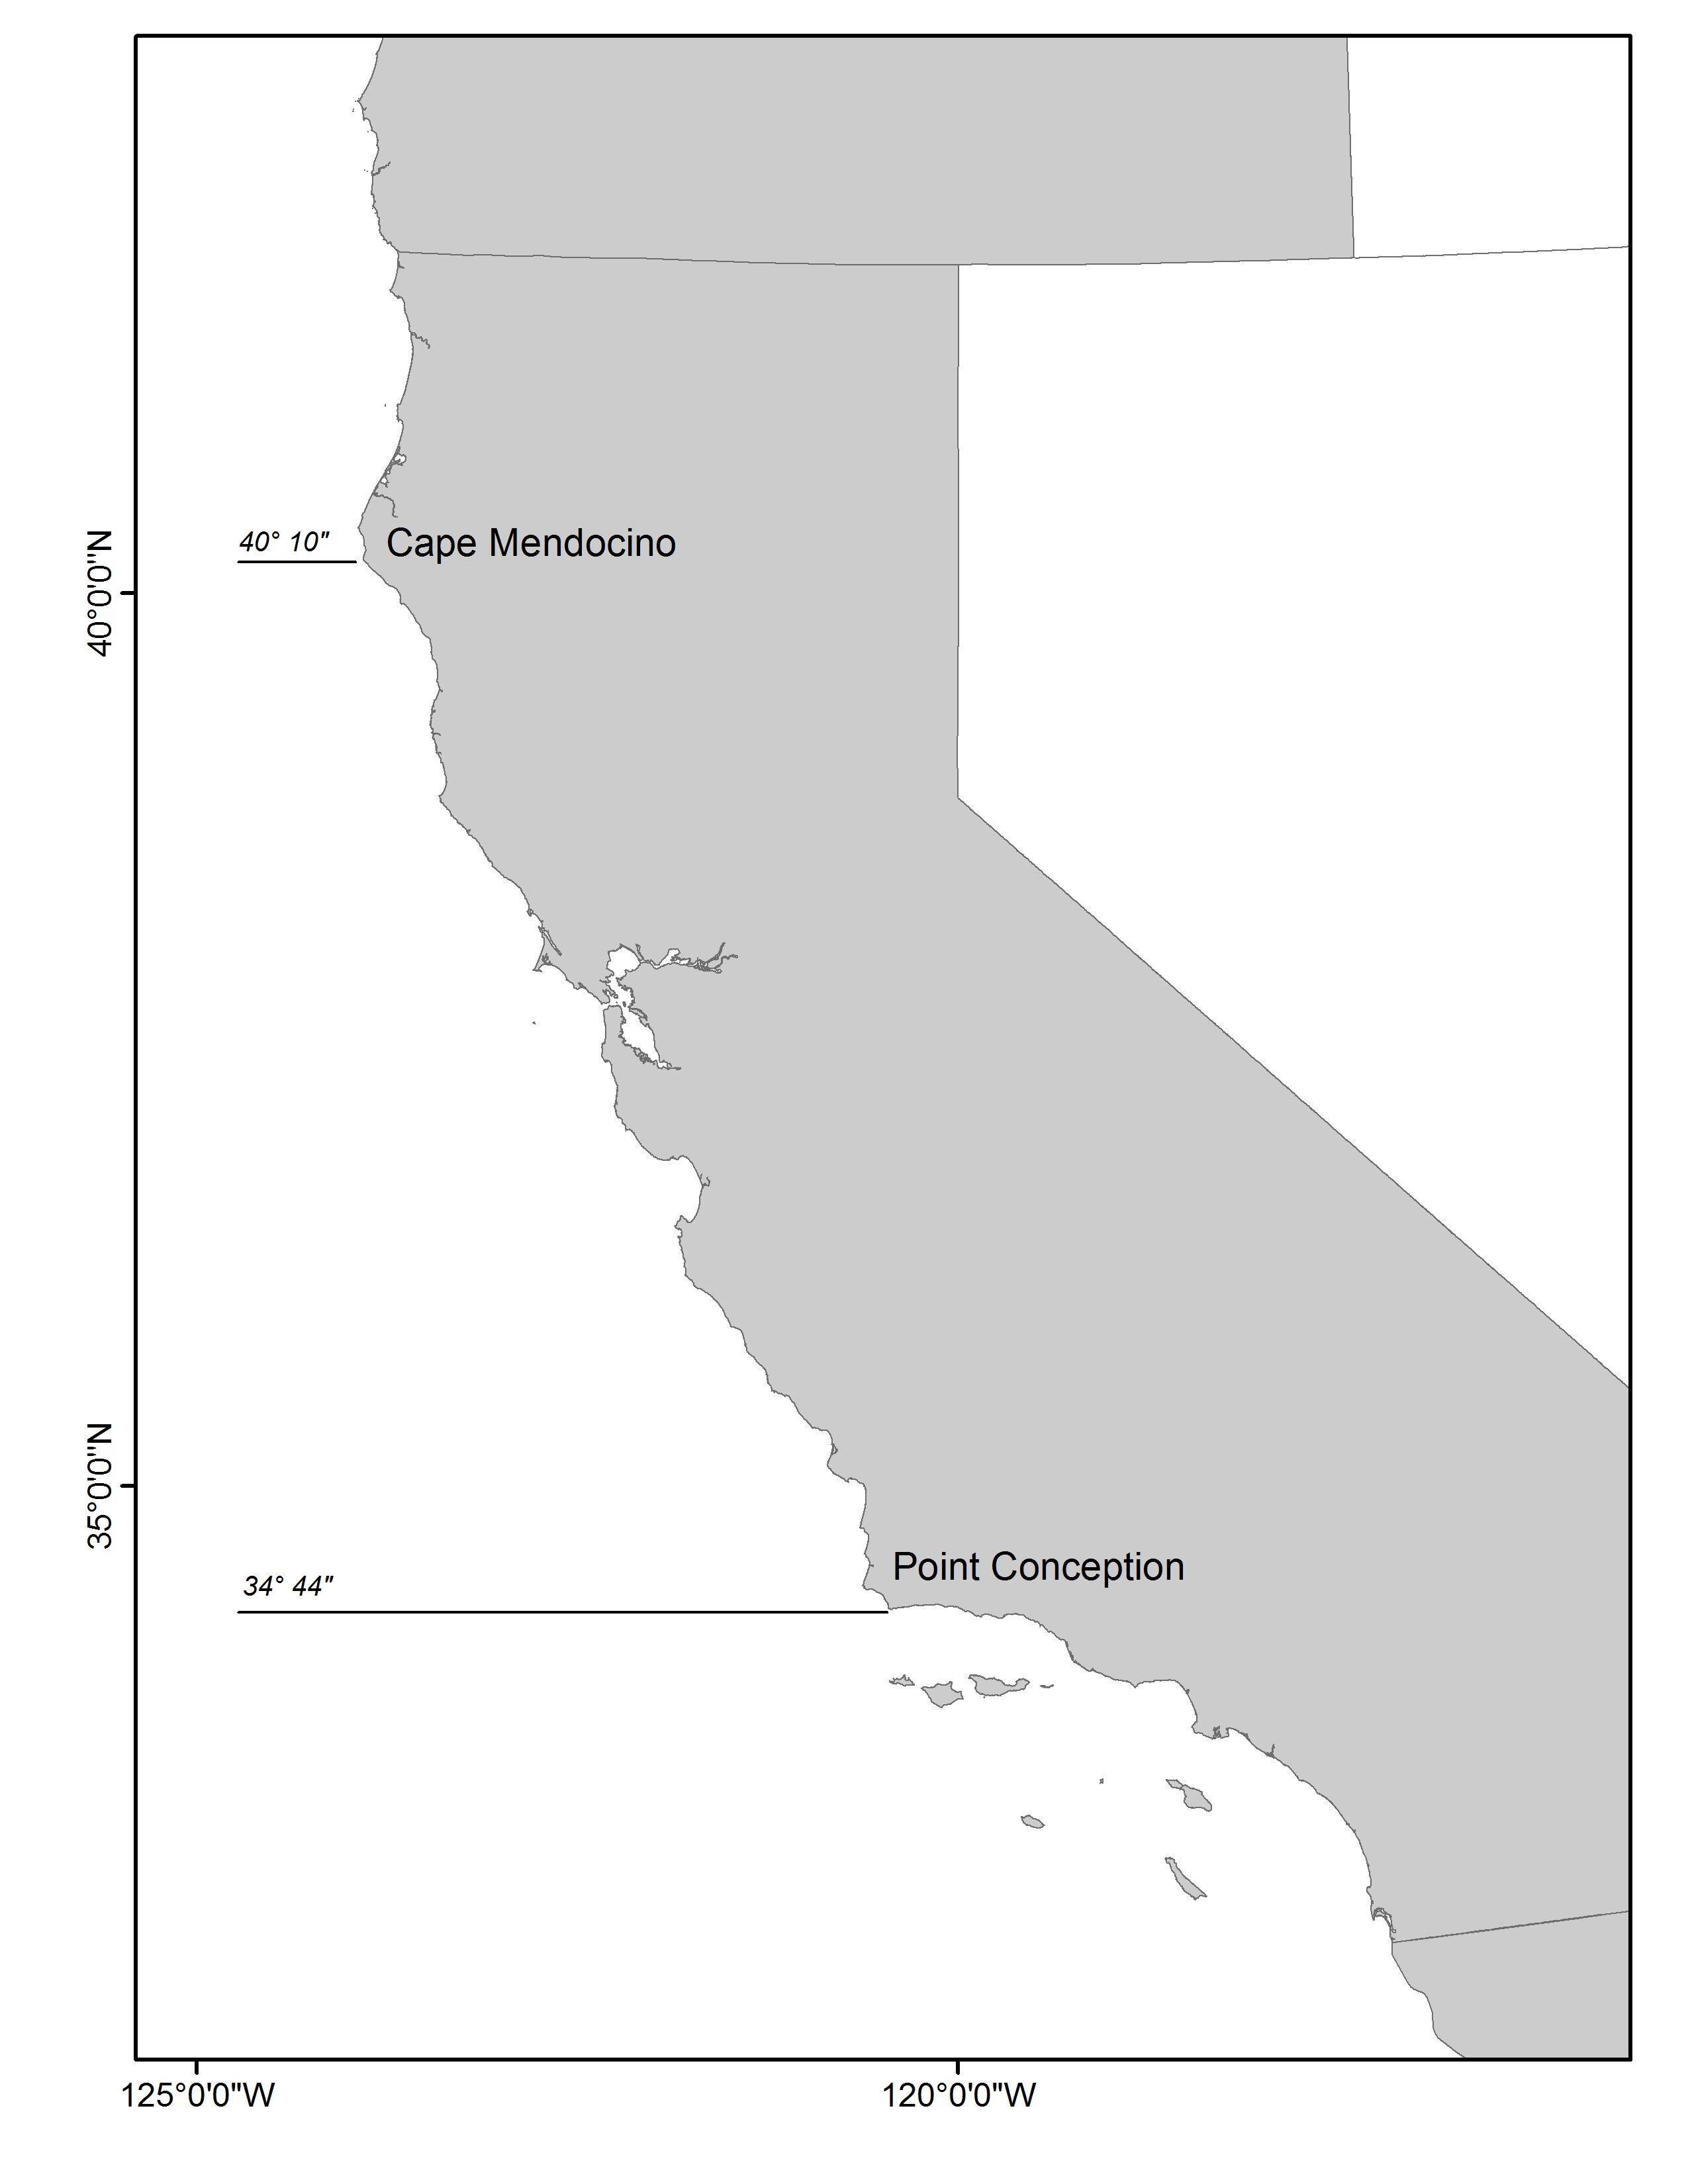
\includegraphics{Figures/assess_region_map.png}
\caption{Map showing the management area for gopher and black-and-yellow
rockfish from Cape Mendocino to the U.S.-Mexico border.
\label{fig:assess_region_map1}}
\end{figure}

\begin{figure}
\centering
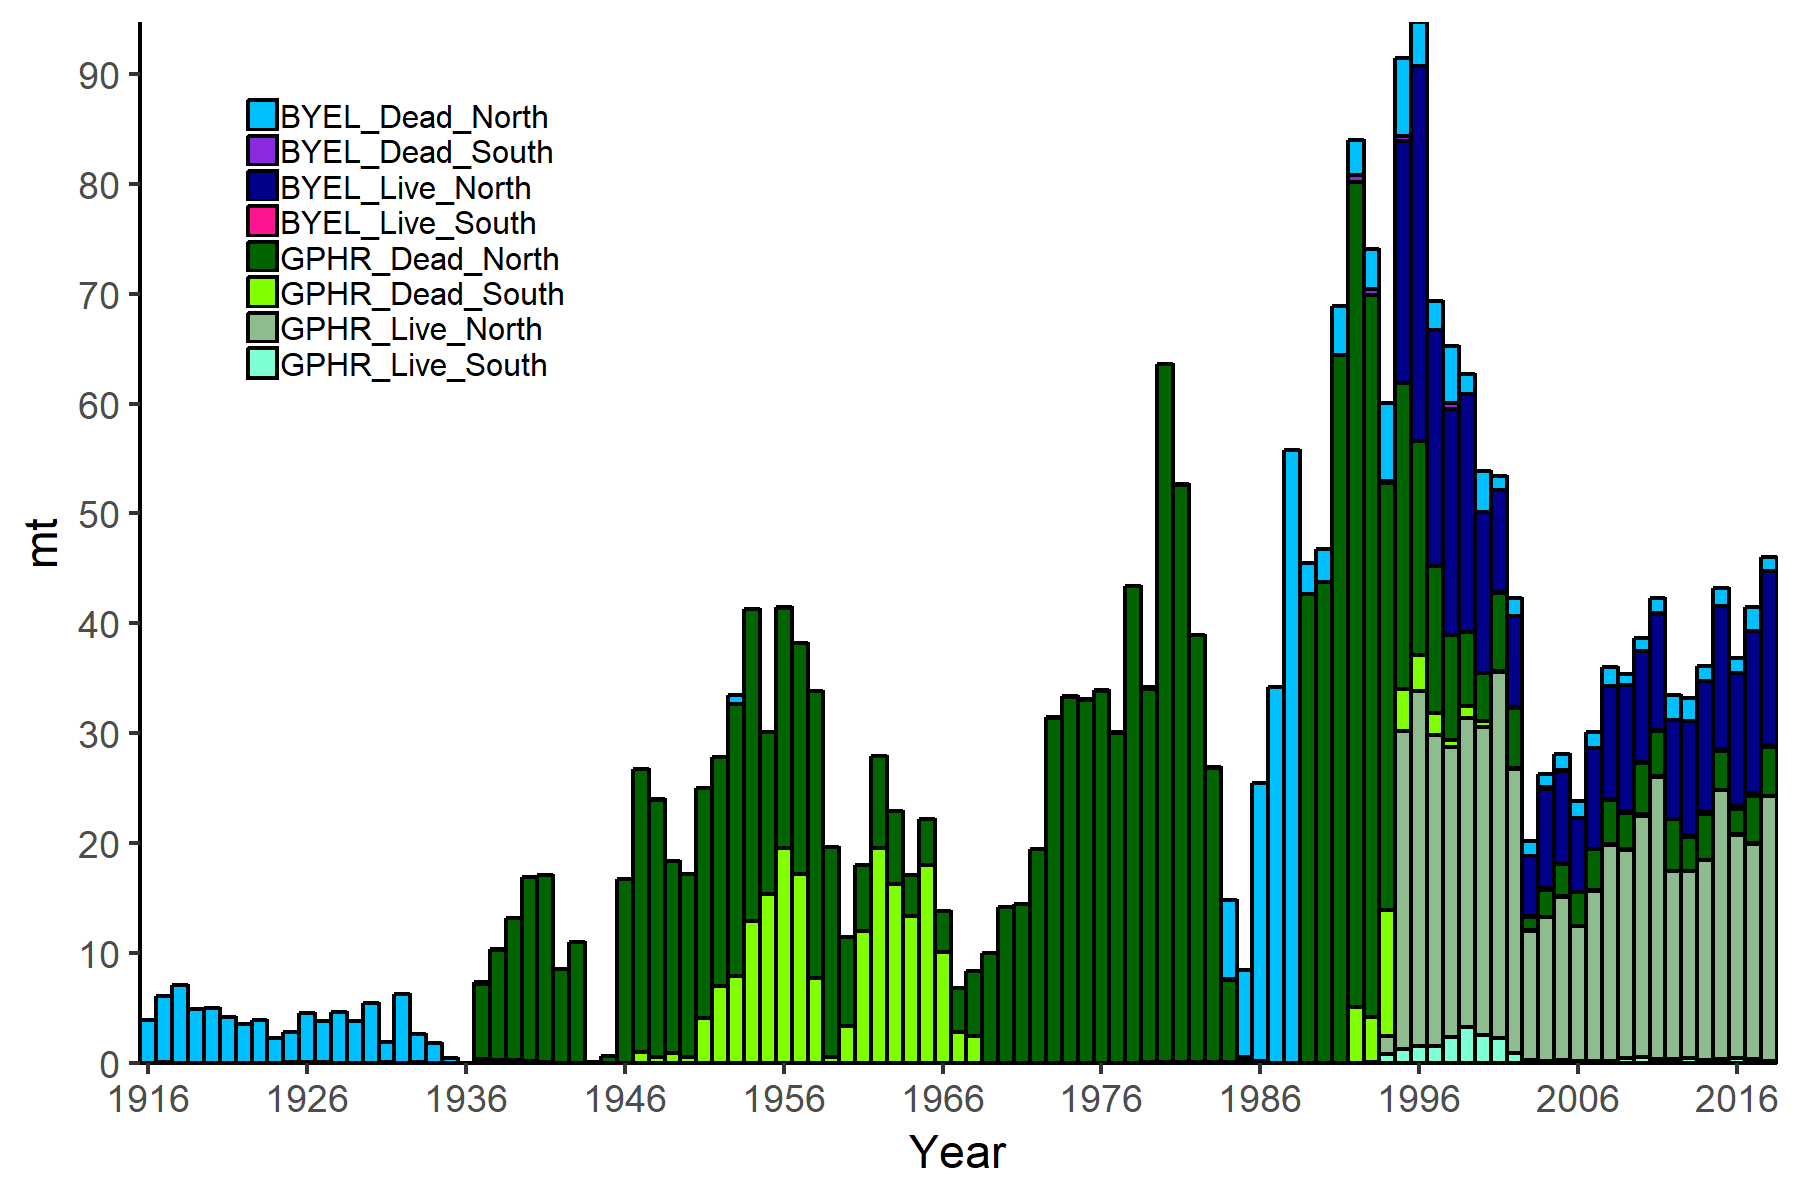
\includegraphics{Figures/Catches_livedeadNS_gby.png}
\caption{Commercial landings for gopher (GPHR) and black-and-yellow
(BYEL) rockfishes landed live and dead north and south of Point
Conception. All catch time series were combined for the assessment into
one commercial fleet. \label{fig:Catches_livedeadNS_gby}}
\end{figure}

\begin{figure}
\centering
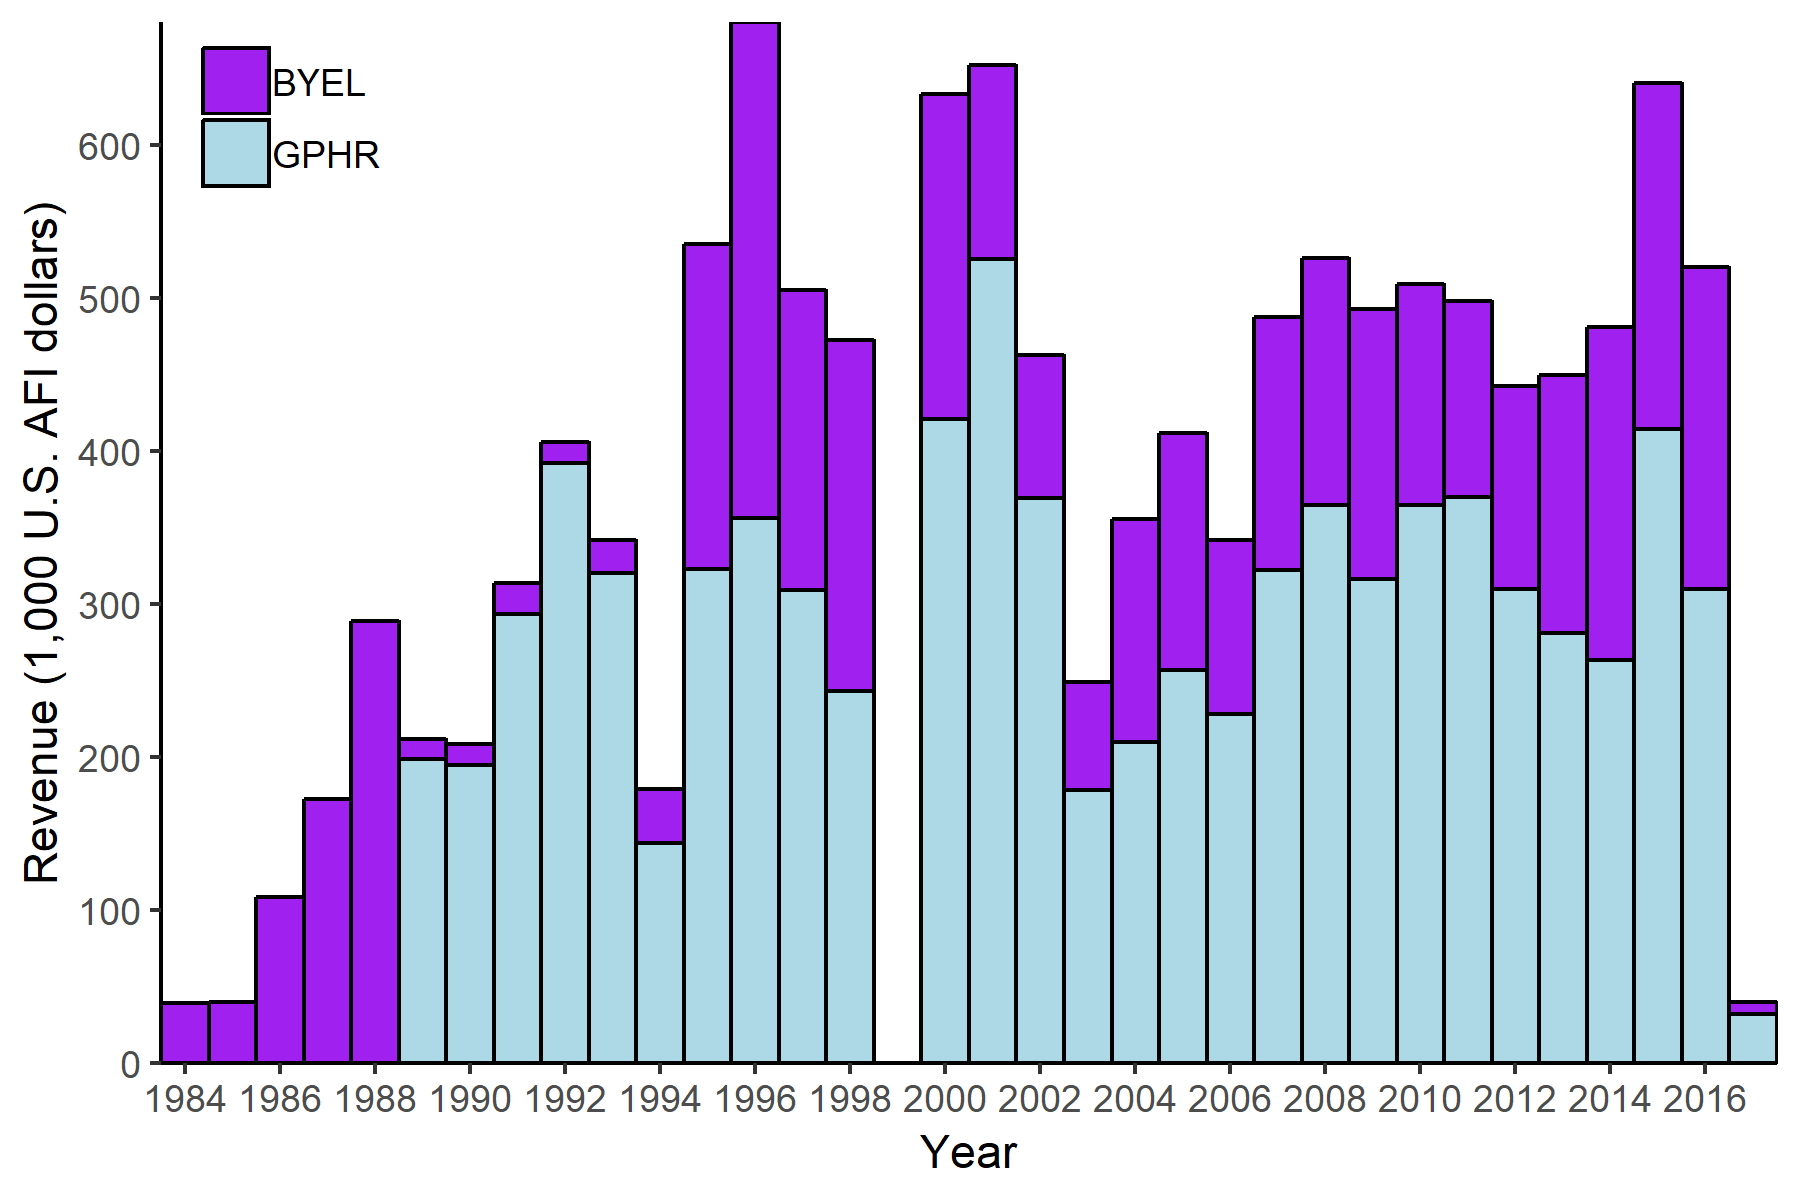
\includegraphics{Figures/GBY_revenue.png}
\caption{Annual ex-vessel revenue, adjusted for inflation (AFI) in
thousands of dollars for gopher and black-and-yellow rockfish.
\label{fig:GBY_revenue}}
\end{figure}

\begin{figure}
\centering
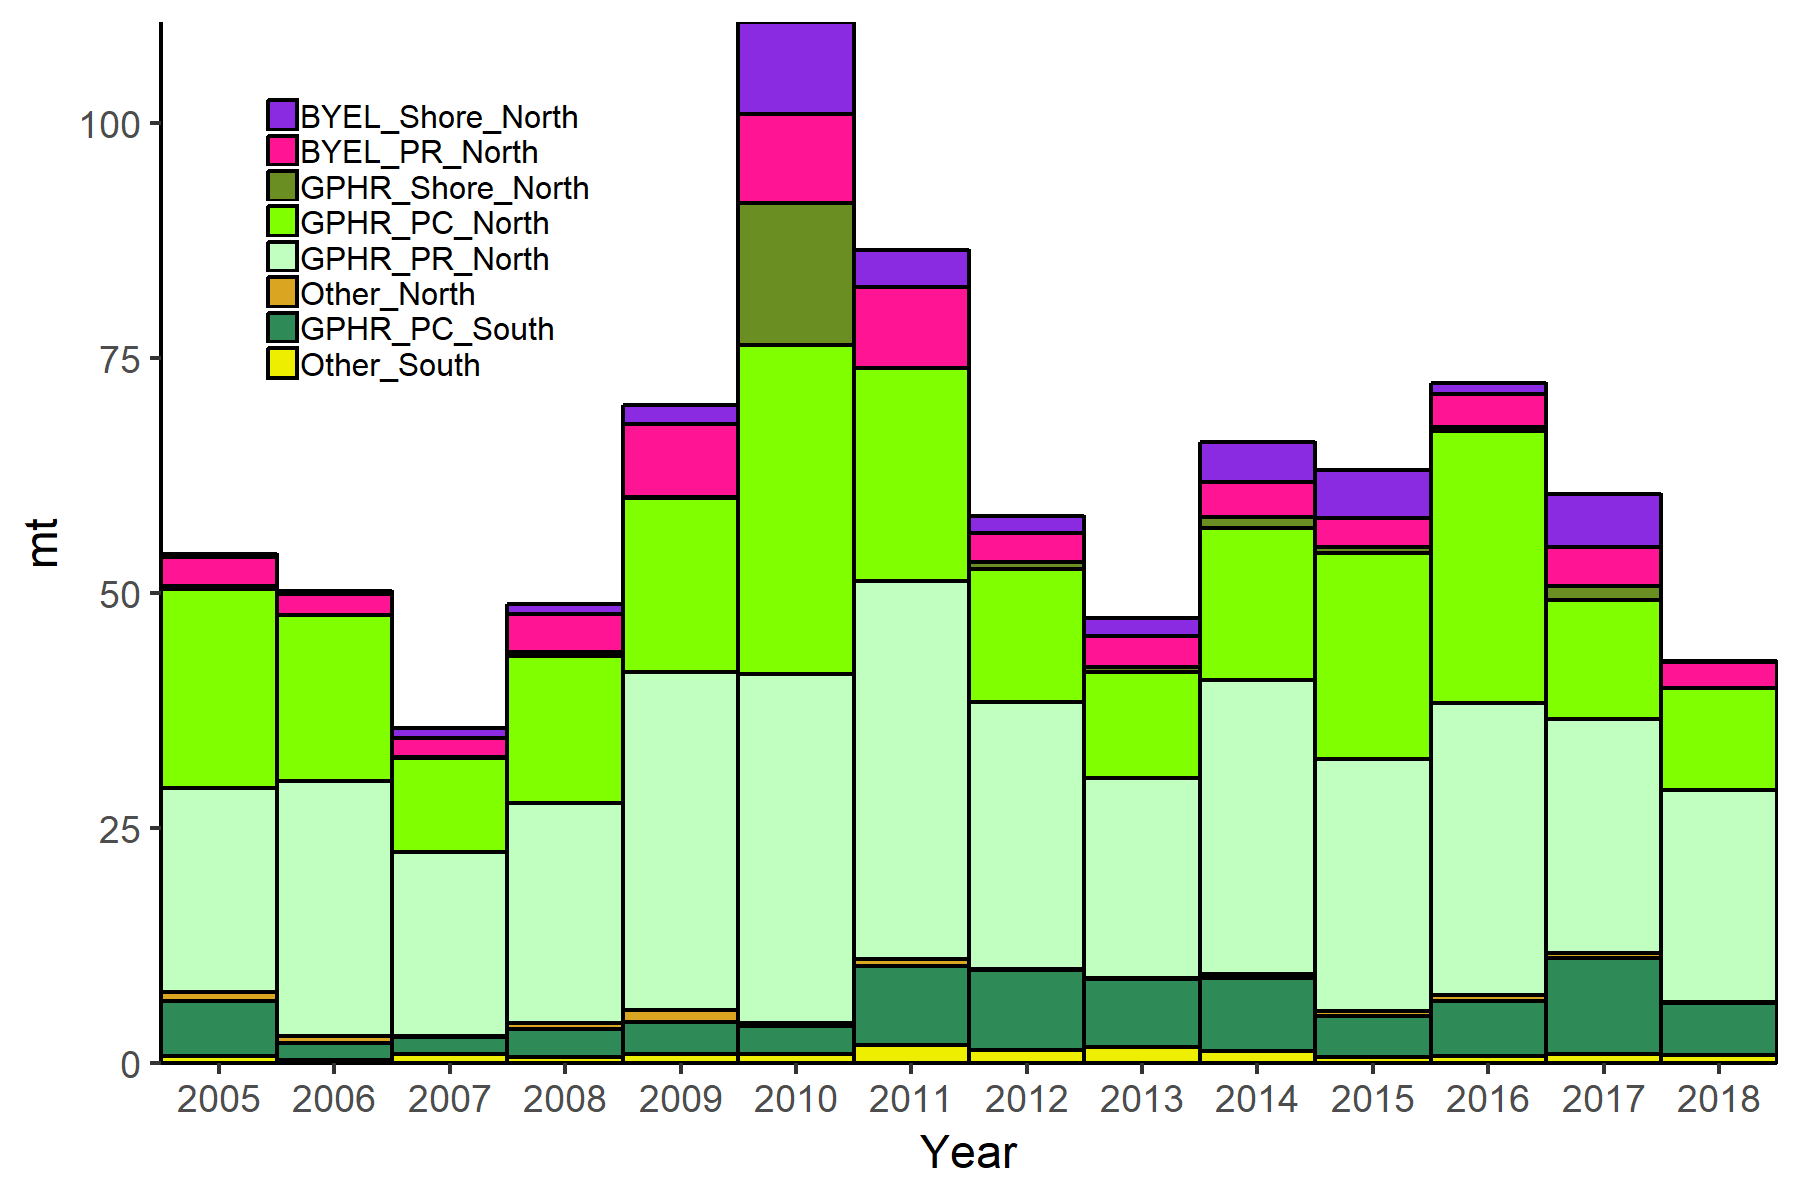
\includegraphics{Figures/CRFS_totalmort_gby.png}
\caption{Recreational total mortality for gopher rockfish (GPHR) and
black-and-yellow (BYEL) rockfish from the CRFS sampling era by mode and
split north and south of Point Conception. \label{fig:CFRS_catches}}
\end{figure}

\begin{figure}
\centering
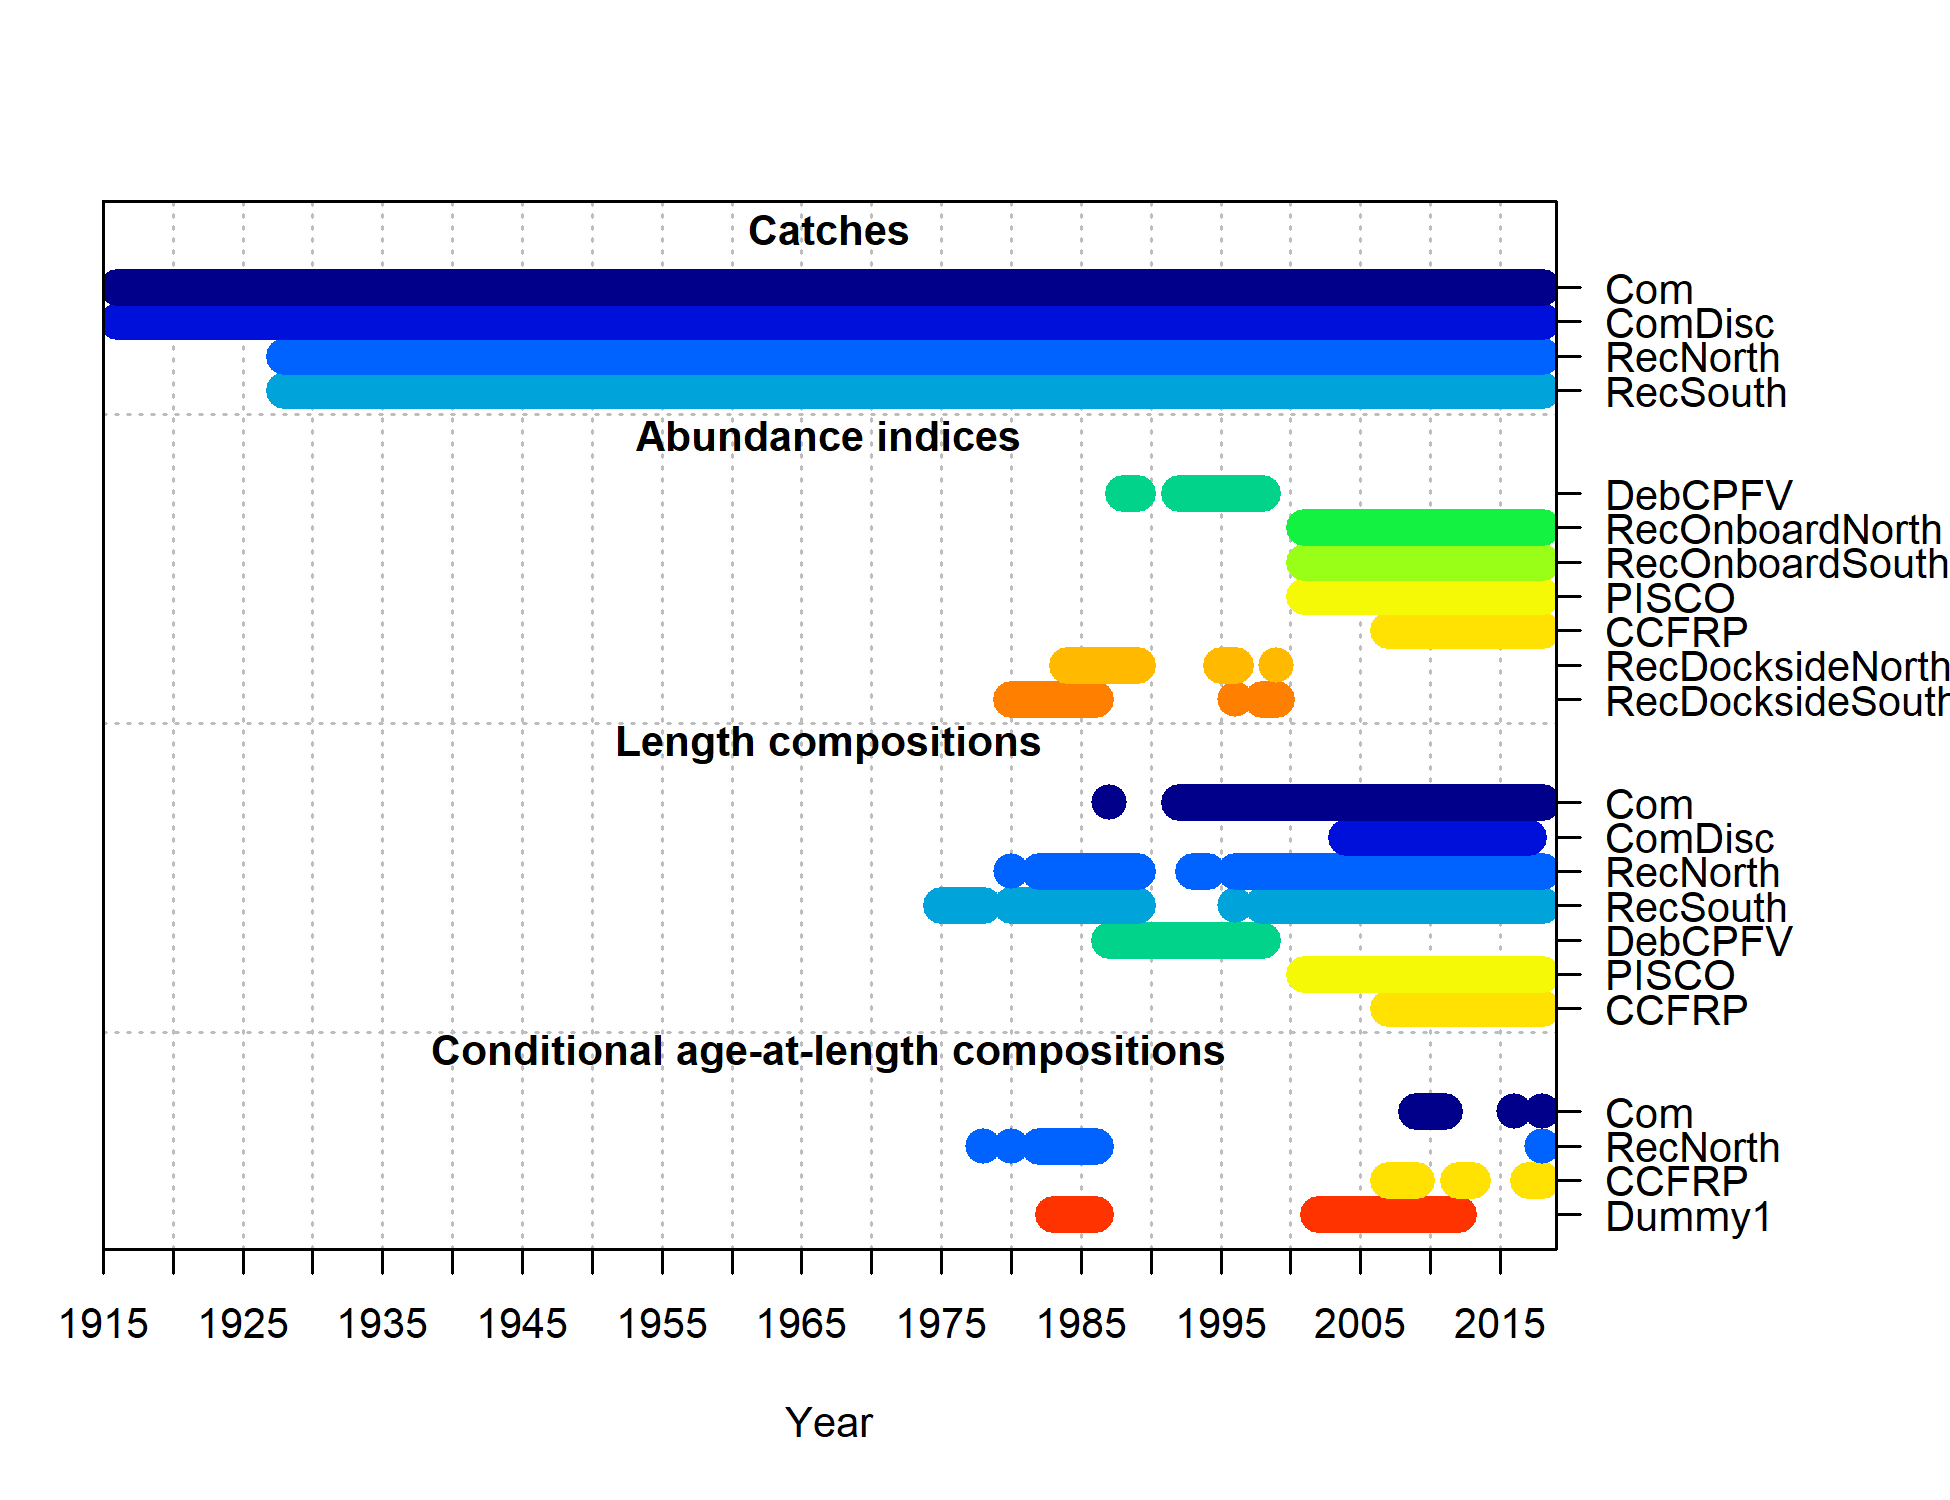
\includegraphics{r4ss/plots_mod1/data_plot.png}
\caption{Summary of data sources used in the model.
\label{fig:data_plot}}
\end{figure}

\begin{figure}
\centering
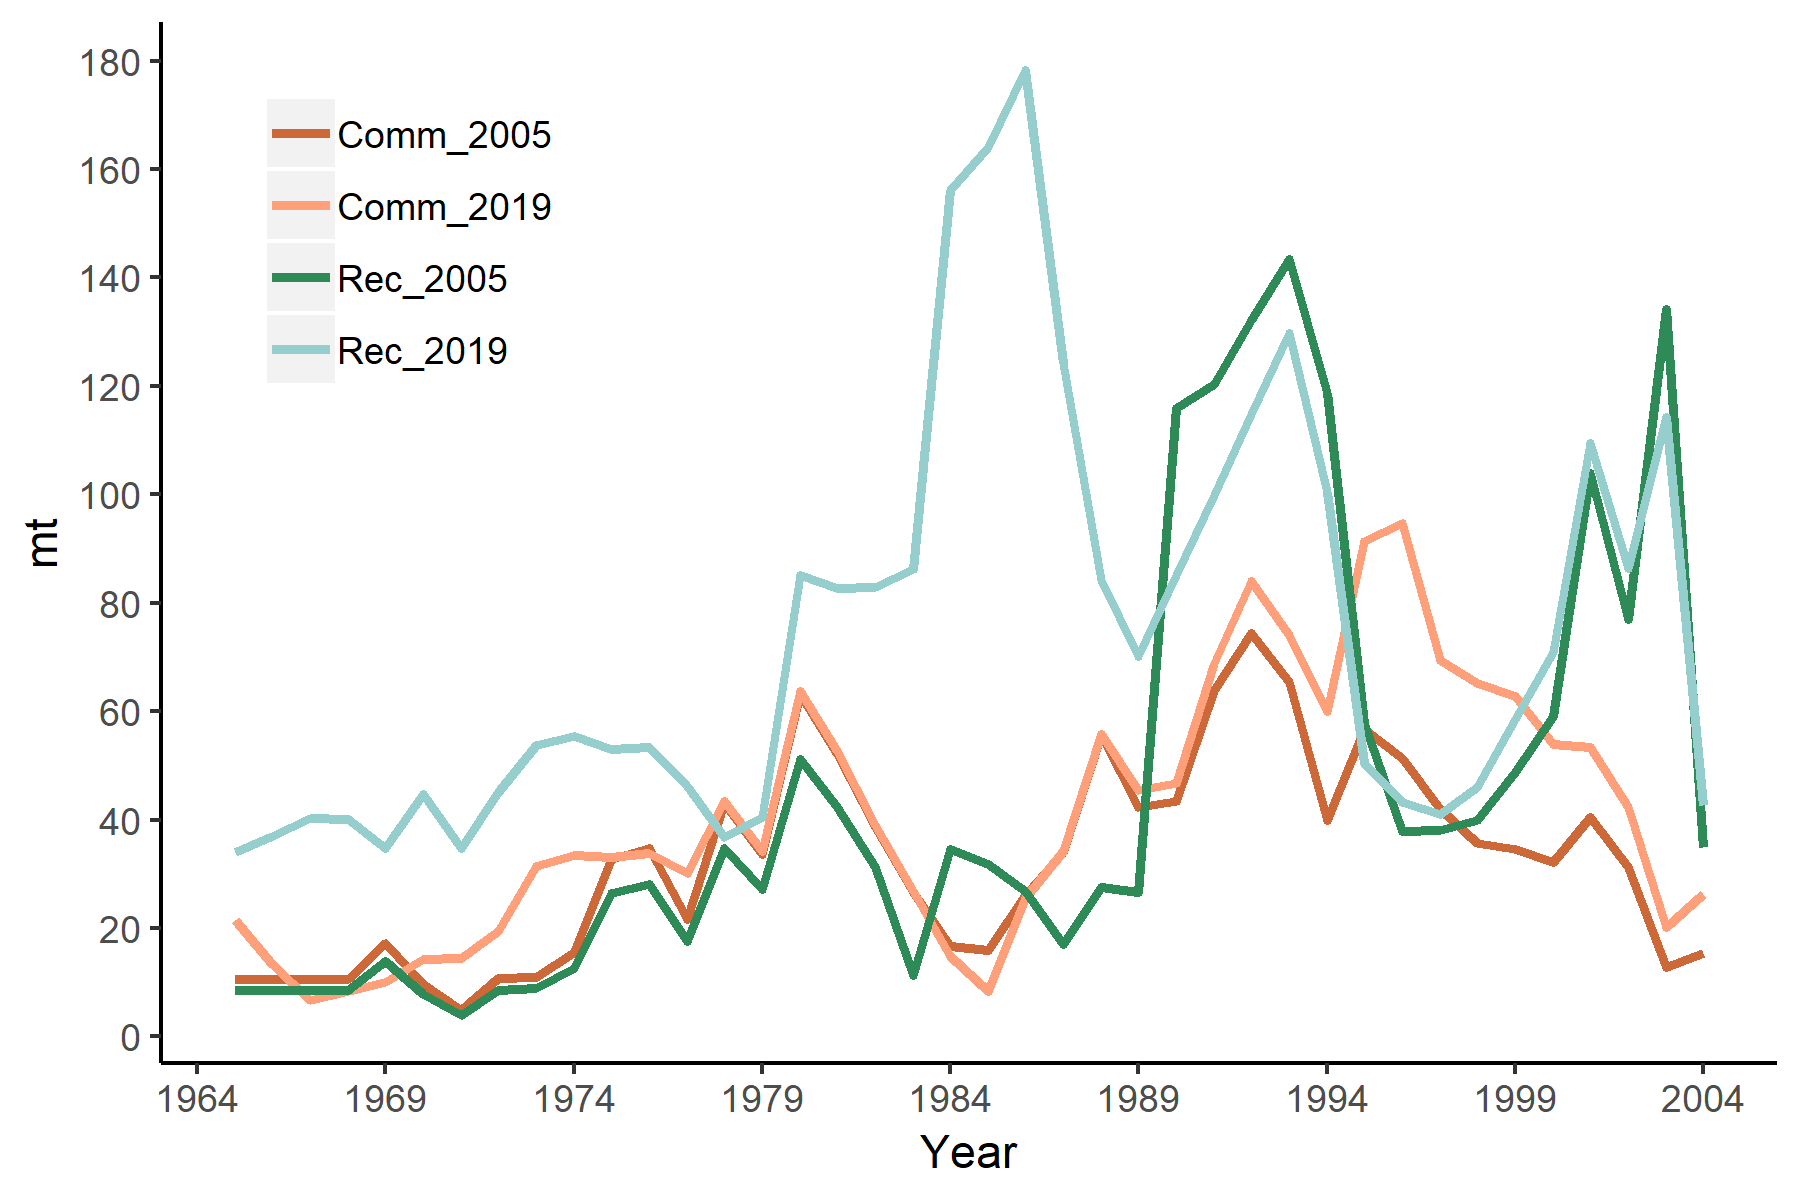
\includegraphics{Figures/assessment_compare.png}
\caption{Comparison of the recreational and commercial fishery landings
from the 2005 assessment to this 2019 assessment. Note that the 2019
assessment includes both gopher and black-and-yellow rockfish where the
2005 assessment represents gopher rockfish only. The 2005 assessment
also did not include landings from south of Point Conception.
\label{fig:Assessment_compare}}
\end{figure}

\begin{figure}
\centering
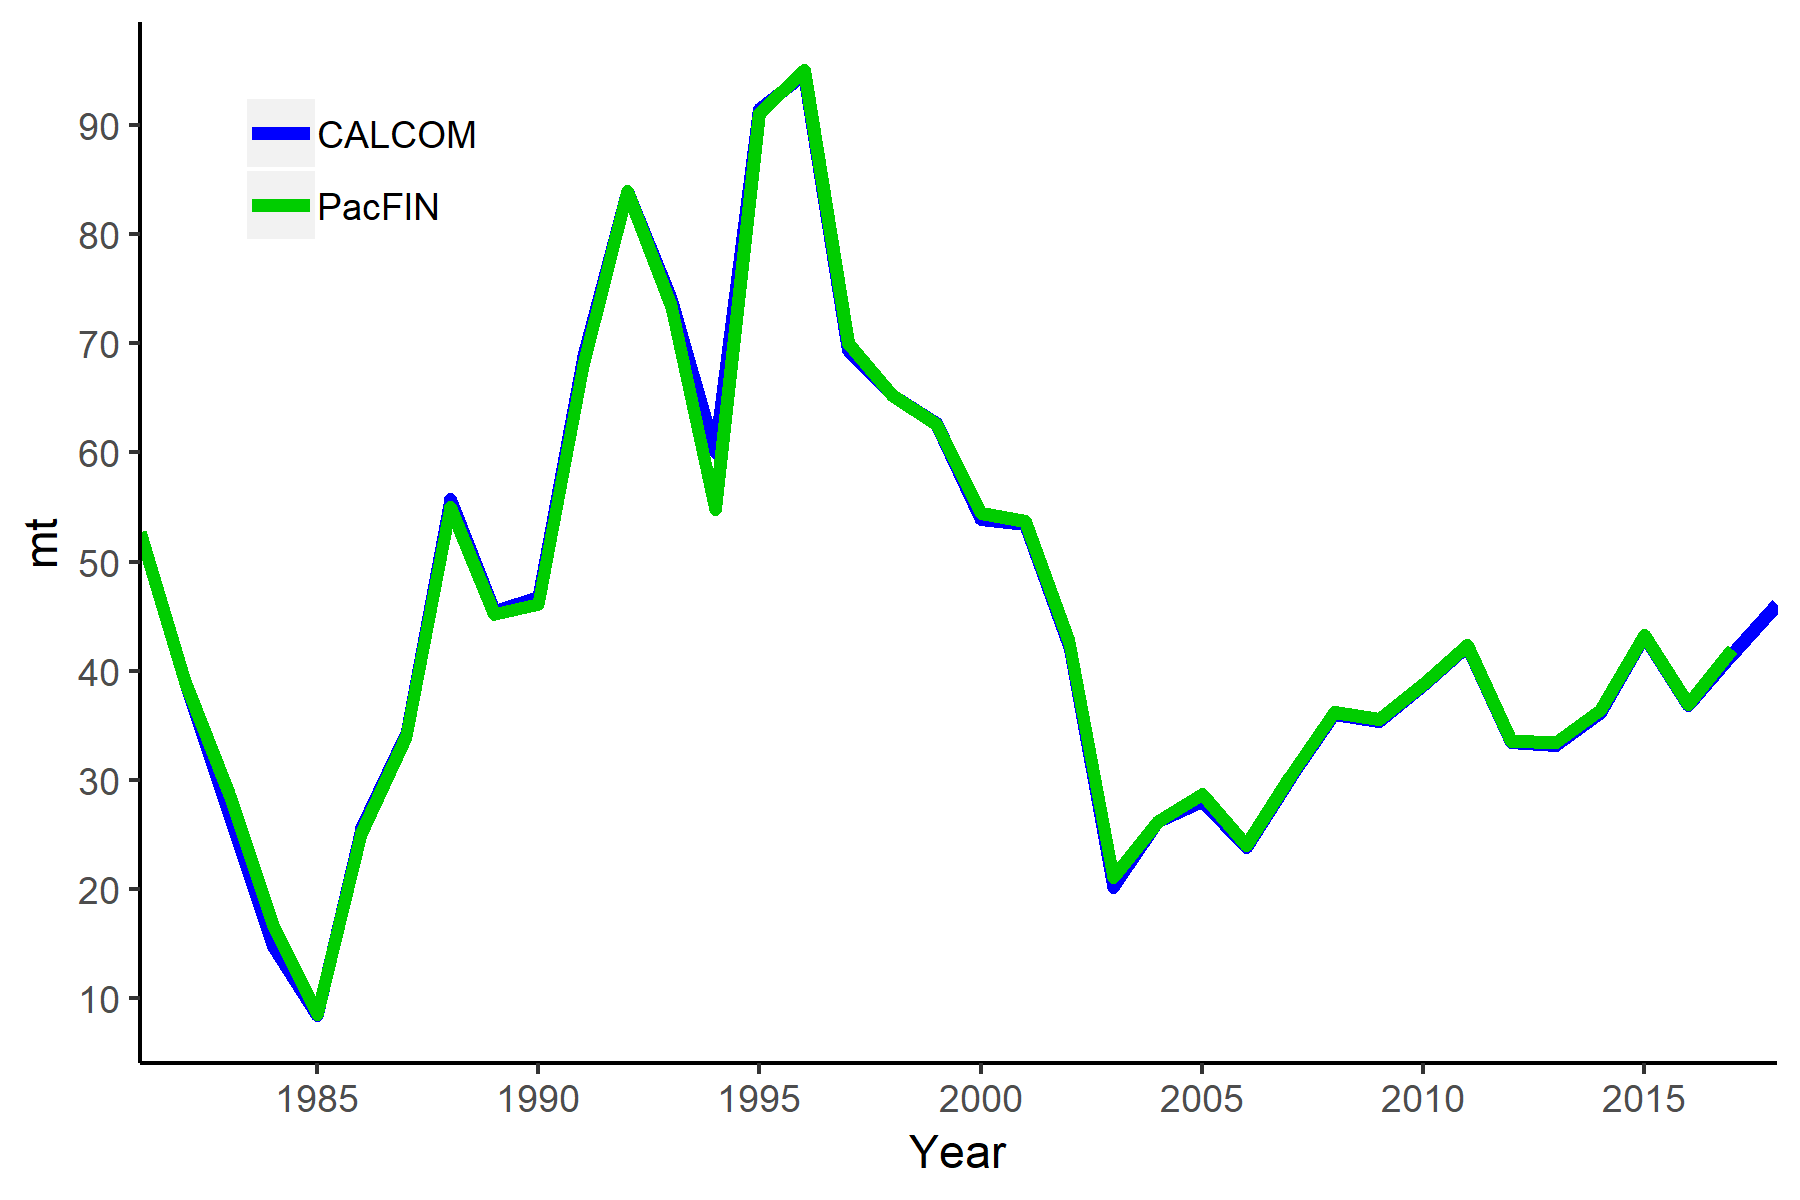
\includegraphics{Figures/Calcom_vs_Pacfin.png}
\caption{Commercial landings estimates from CALCOM and PacFIN.
\label{fig:Calcom_vs_Pacfin}}
\end{figure}

\begin{figure}
\centering
\includegraphics{Figures/Calcom_vs_pacfin_lengths.png}
\caption{Percent differences in the expanded length compositions by year
from CALCOM and PacFIN. The same market categories were used for each
dataset, but each database was subject to further independent filtering
criteria and expansion algorithms. \label{fig:Calcom_vs_pacfin_lengths}}
\end{figure}

\begin{figure}
\centering
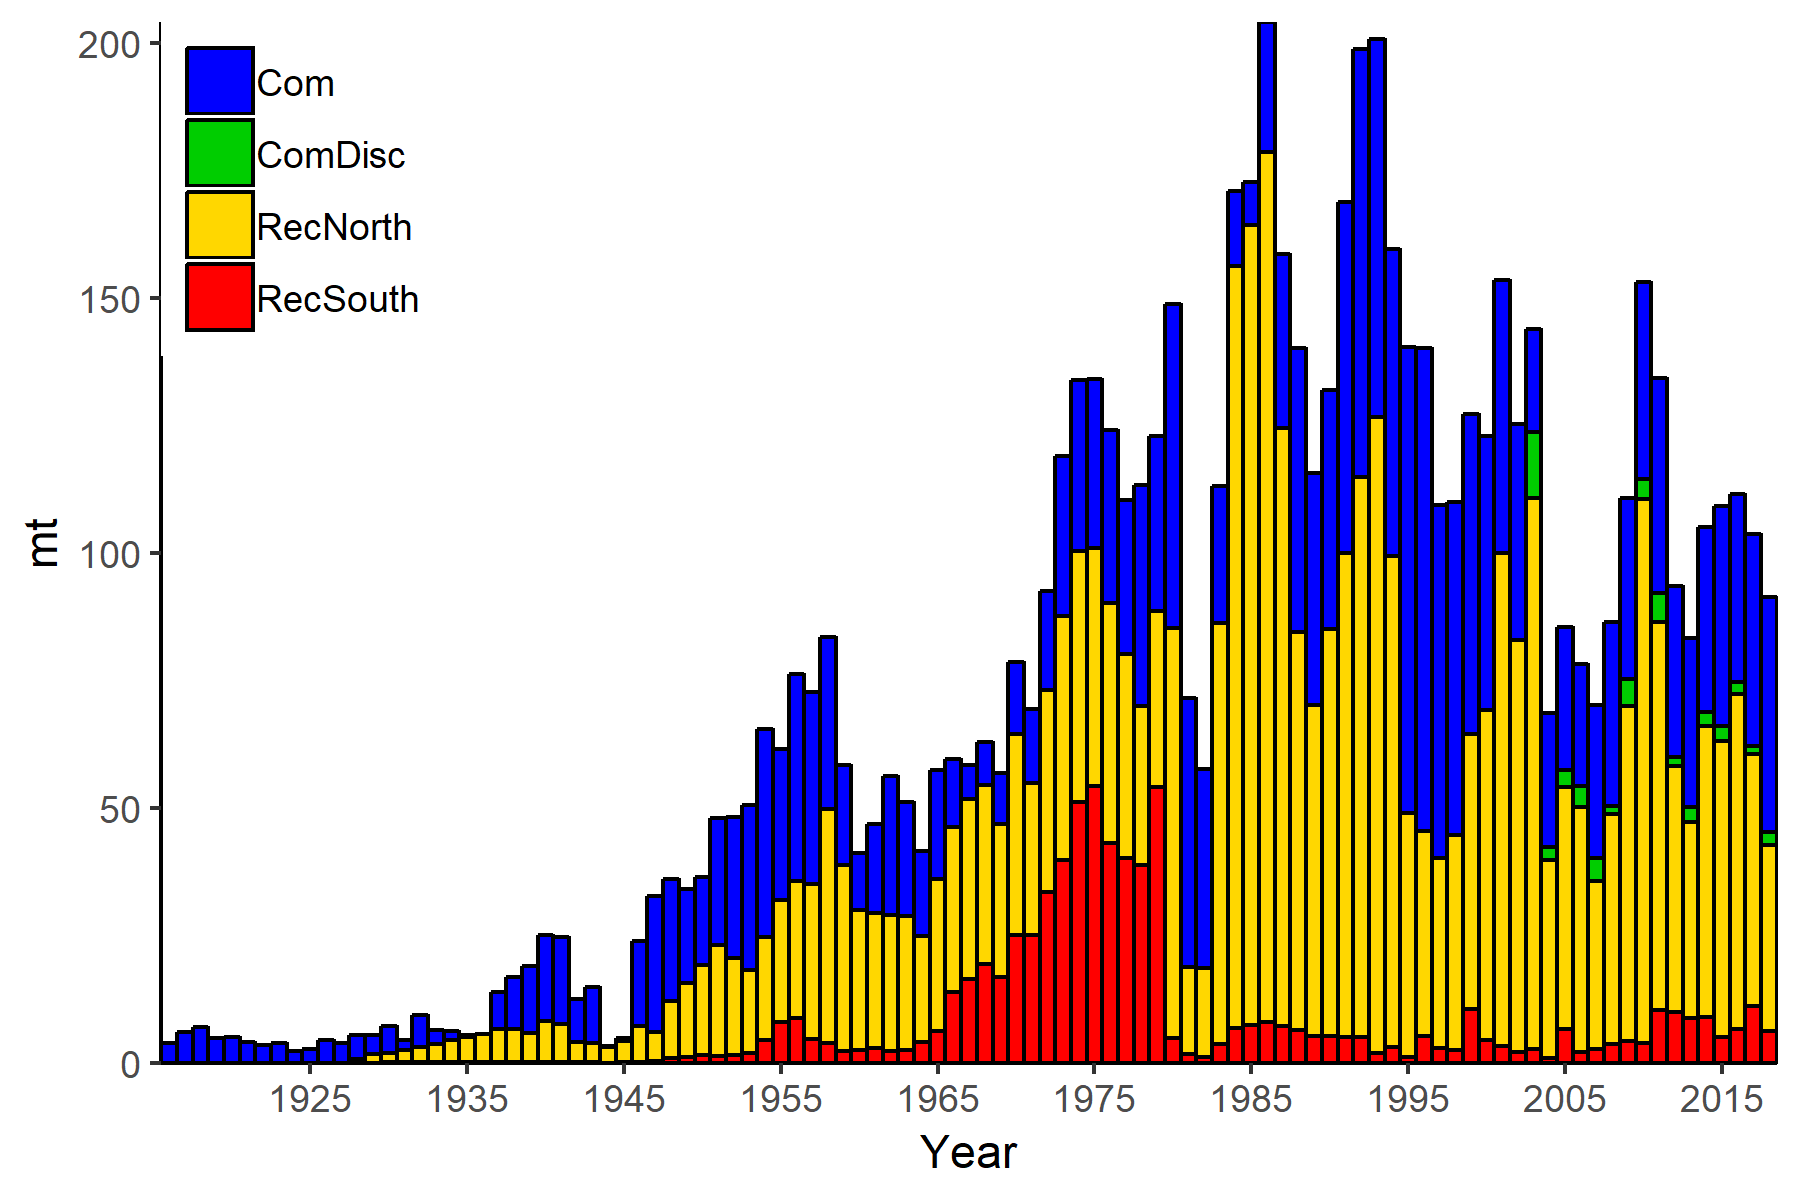
\includegraphics{Figures/Catches_original.png}
\caption{Commercial and recreational landings estimates prior to any
data modification or interpolation to the recreational catches or
hindcasting of commercial discards. \label{fig:Catches_original}}
\end{figure}

\begin{figure}
\centering
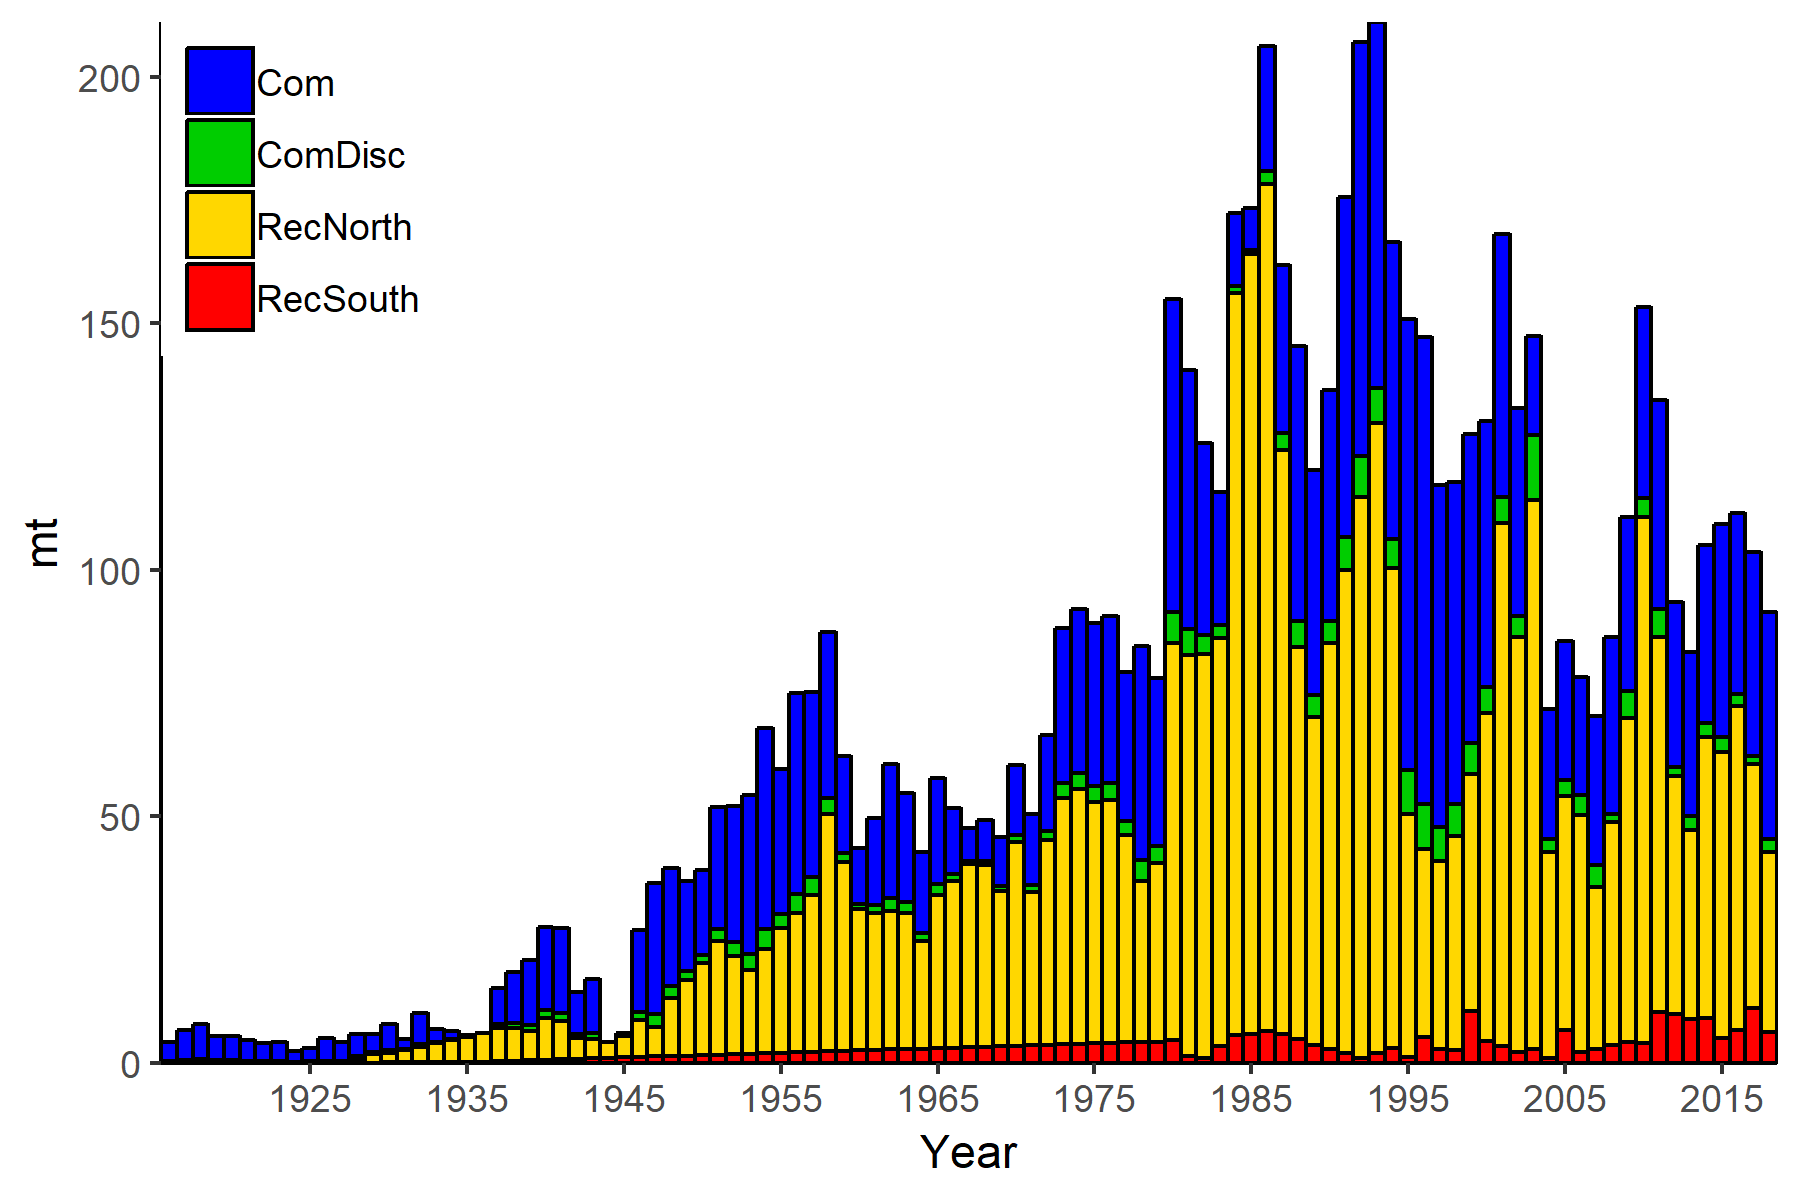
\includegraphics{Figures/Catches_alternate.png}
\caption{Commercial and recreational landings estimates after data
modification and interpolations were made to the recreational catches
and commercial discards. \label{fig:Catches_alternate}}
\end{figure}

\begin{figure}
\centering
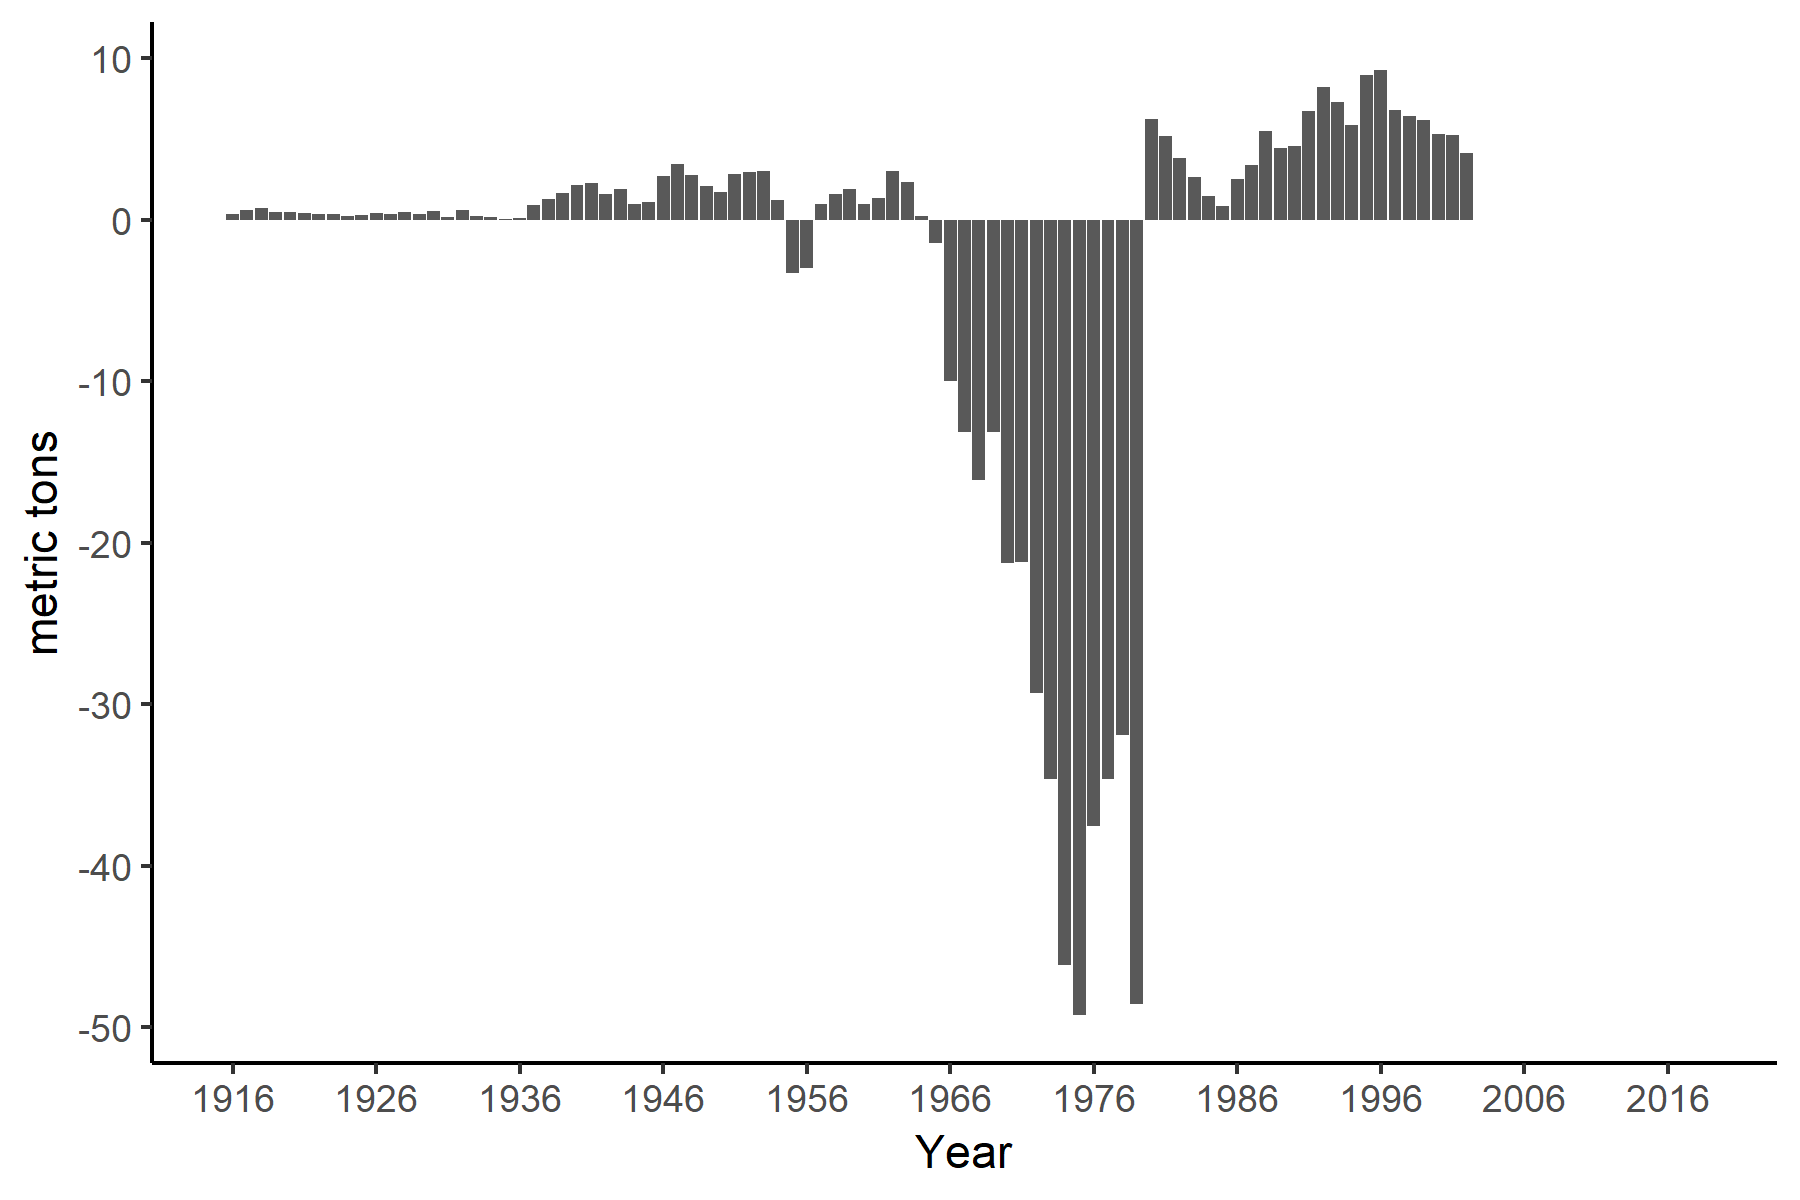
\includegraphics{Figures/catches_difference.png}
\caption{Difference in landings between the original and modified
landings presented in the previous two figures. The only two fleets with
modifications are recreational south and commercial discards. Negative
values indicate catches removed from the original estimates and positive
values represent the addition of landings from the commercial discards.
\label{fig:catches_difference}}
\end{figure}

\FloatBarrier

\begin{figure}
\centering
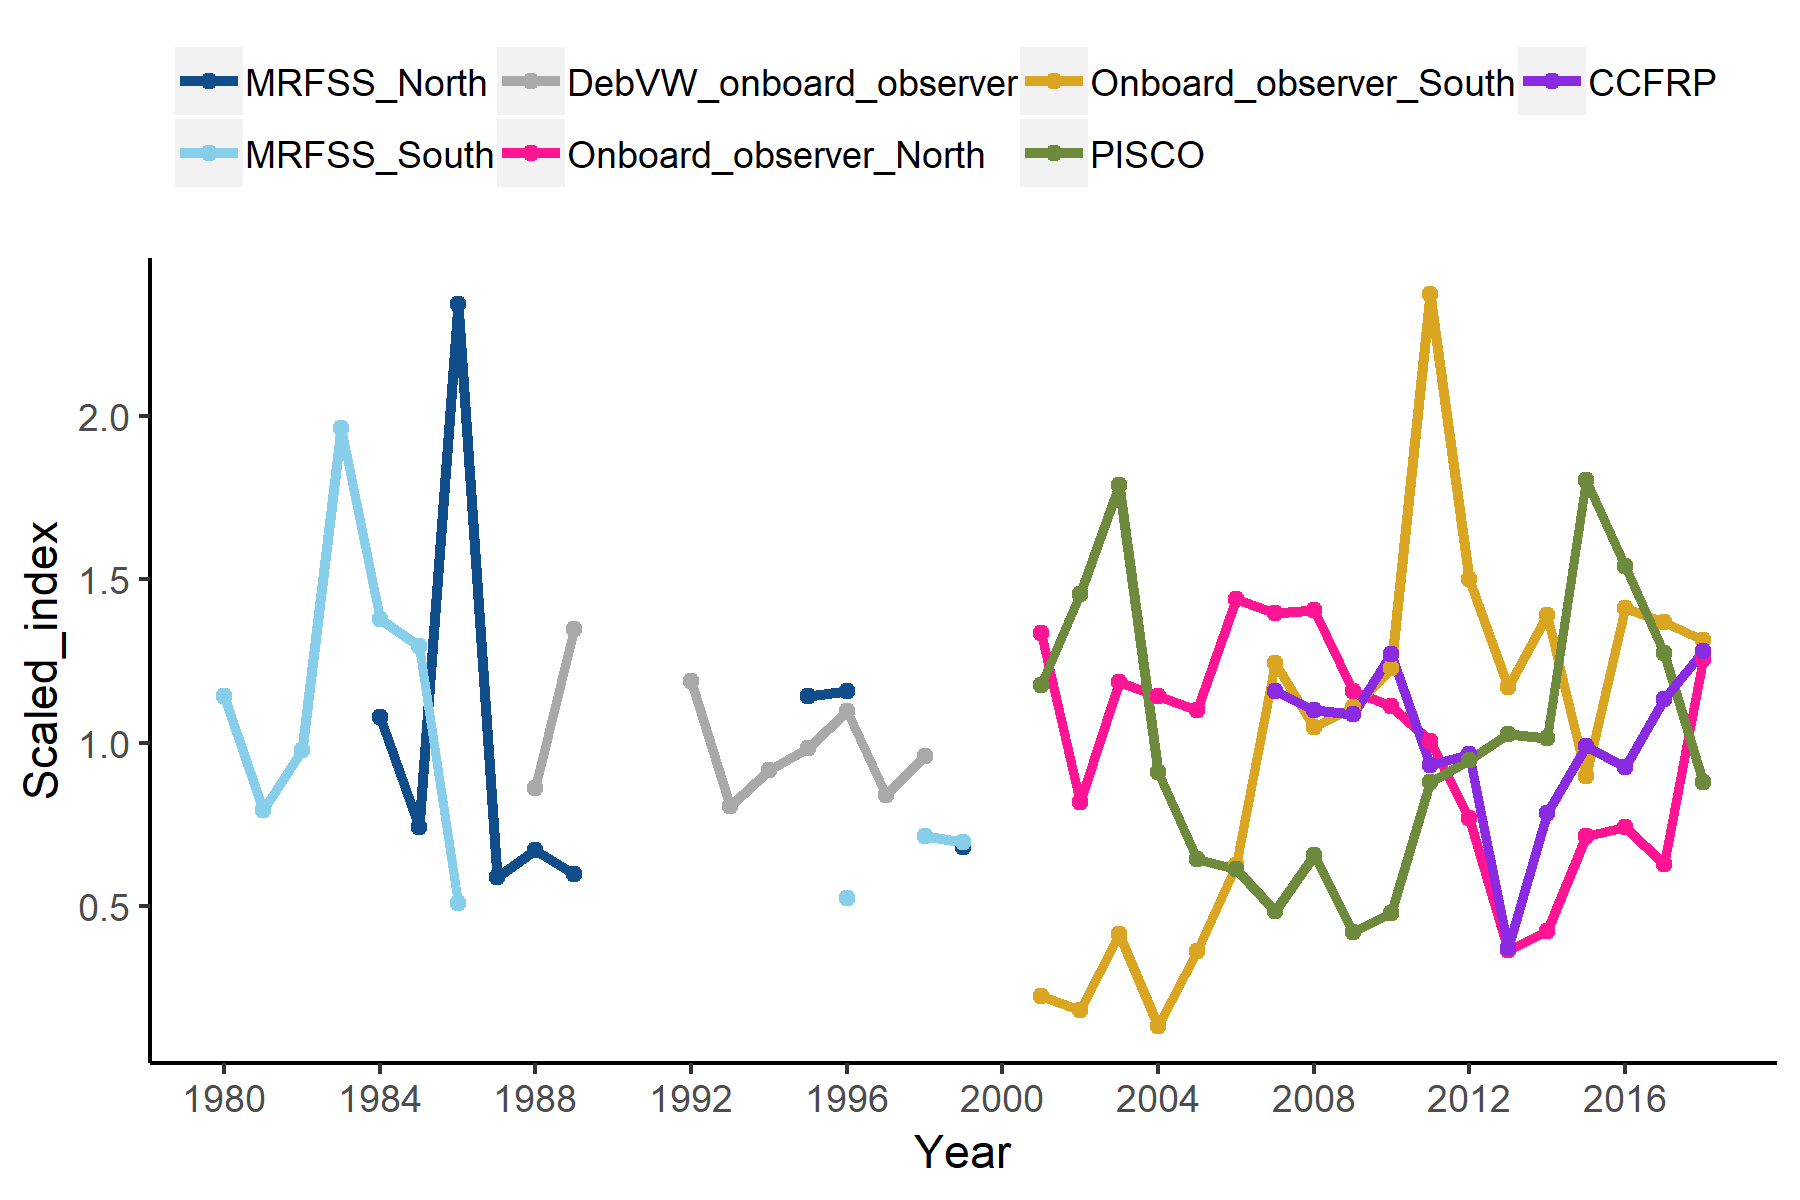
\includegraphics{Figures/All_index_compare.png}
\caption{Comparison of all indices of abundance in the pre-STAR base
model (with each index scaled to its mean).
\label{fig:All_index_compare}}
\end{figure}

\begin{figure}
\centering
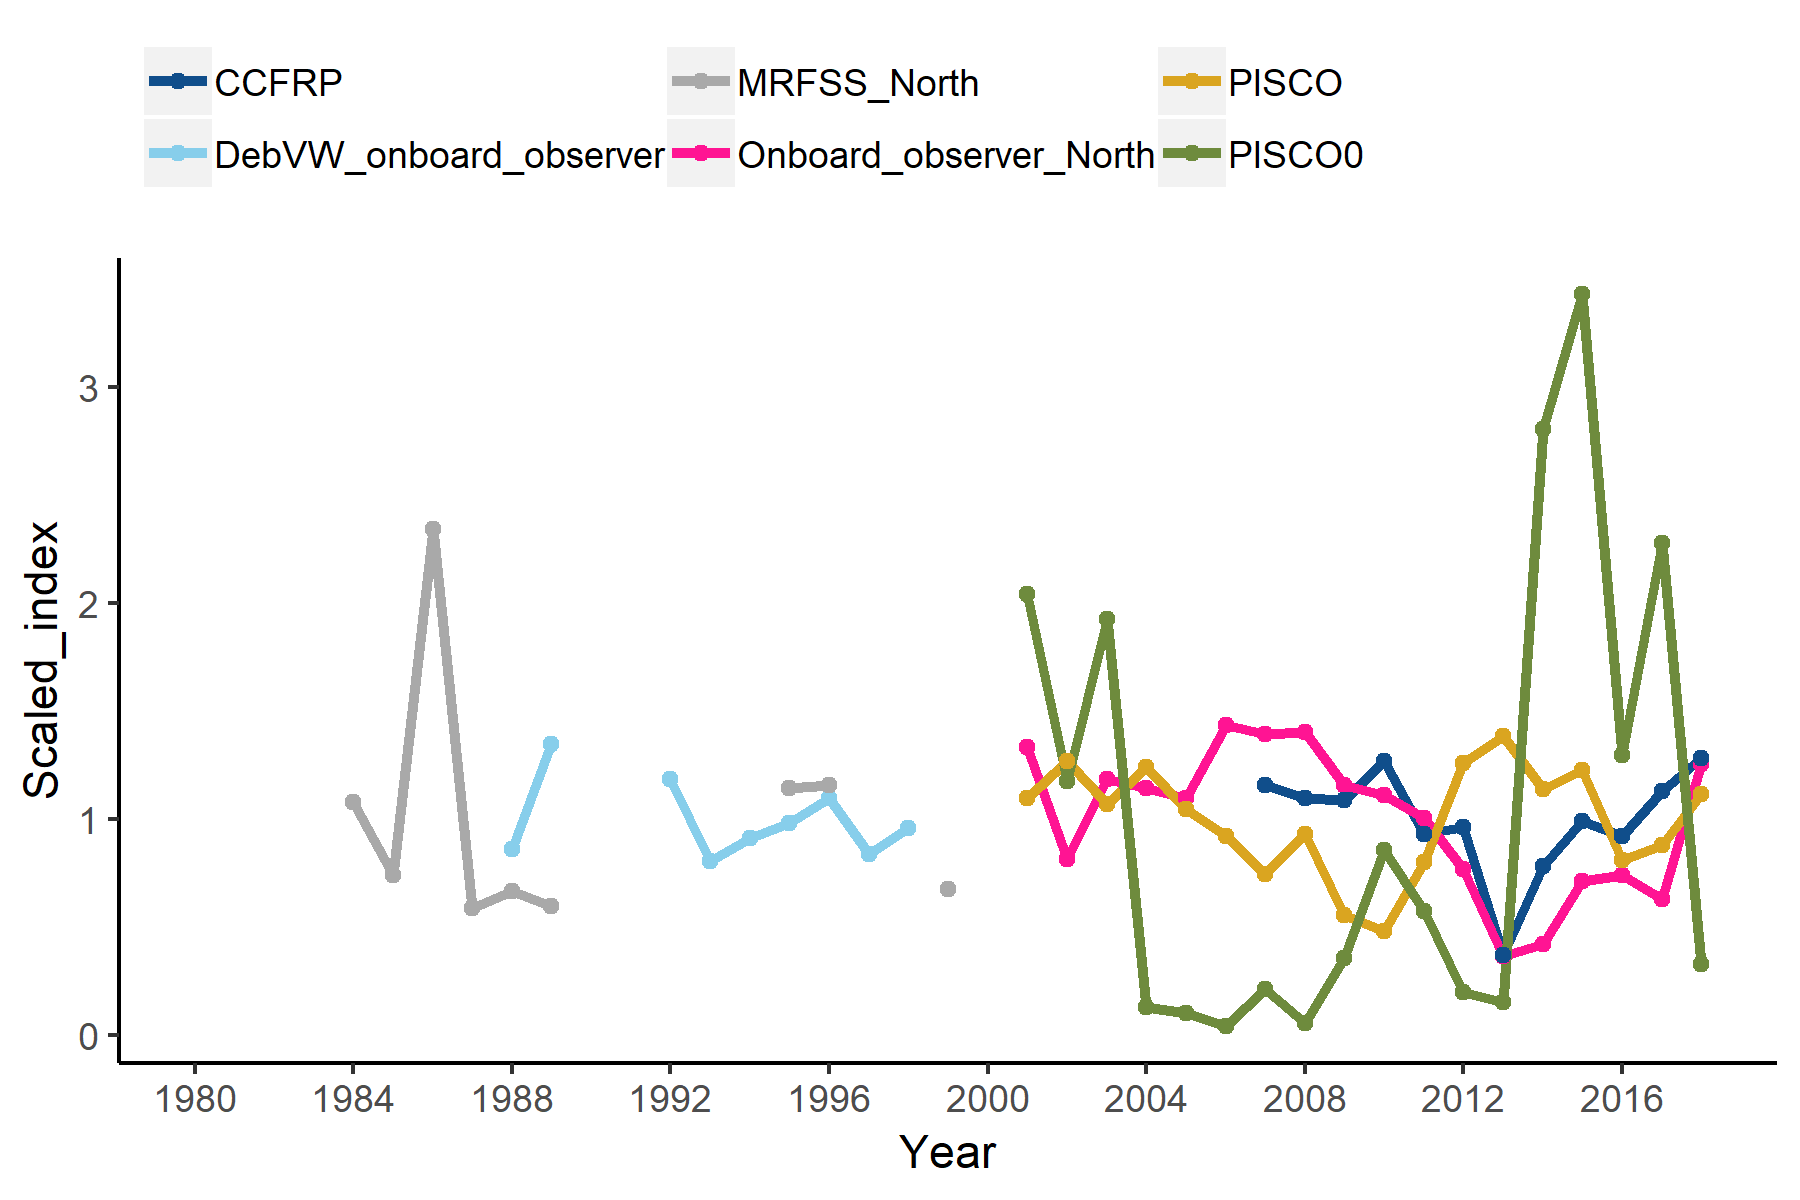
\includegraphics{Figures/All_index_compare_postSTAR.png}
\caption{Comparison of all indices of abundance in the post-STAR base
model (with each index scaled to its mean).
\label{fig:All_index_compare_postSTAR}}
\end{figure}

\begin{figure}
\centering
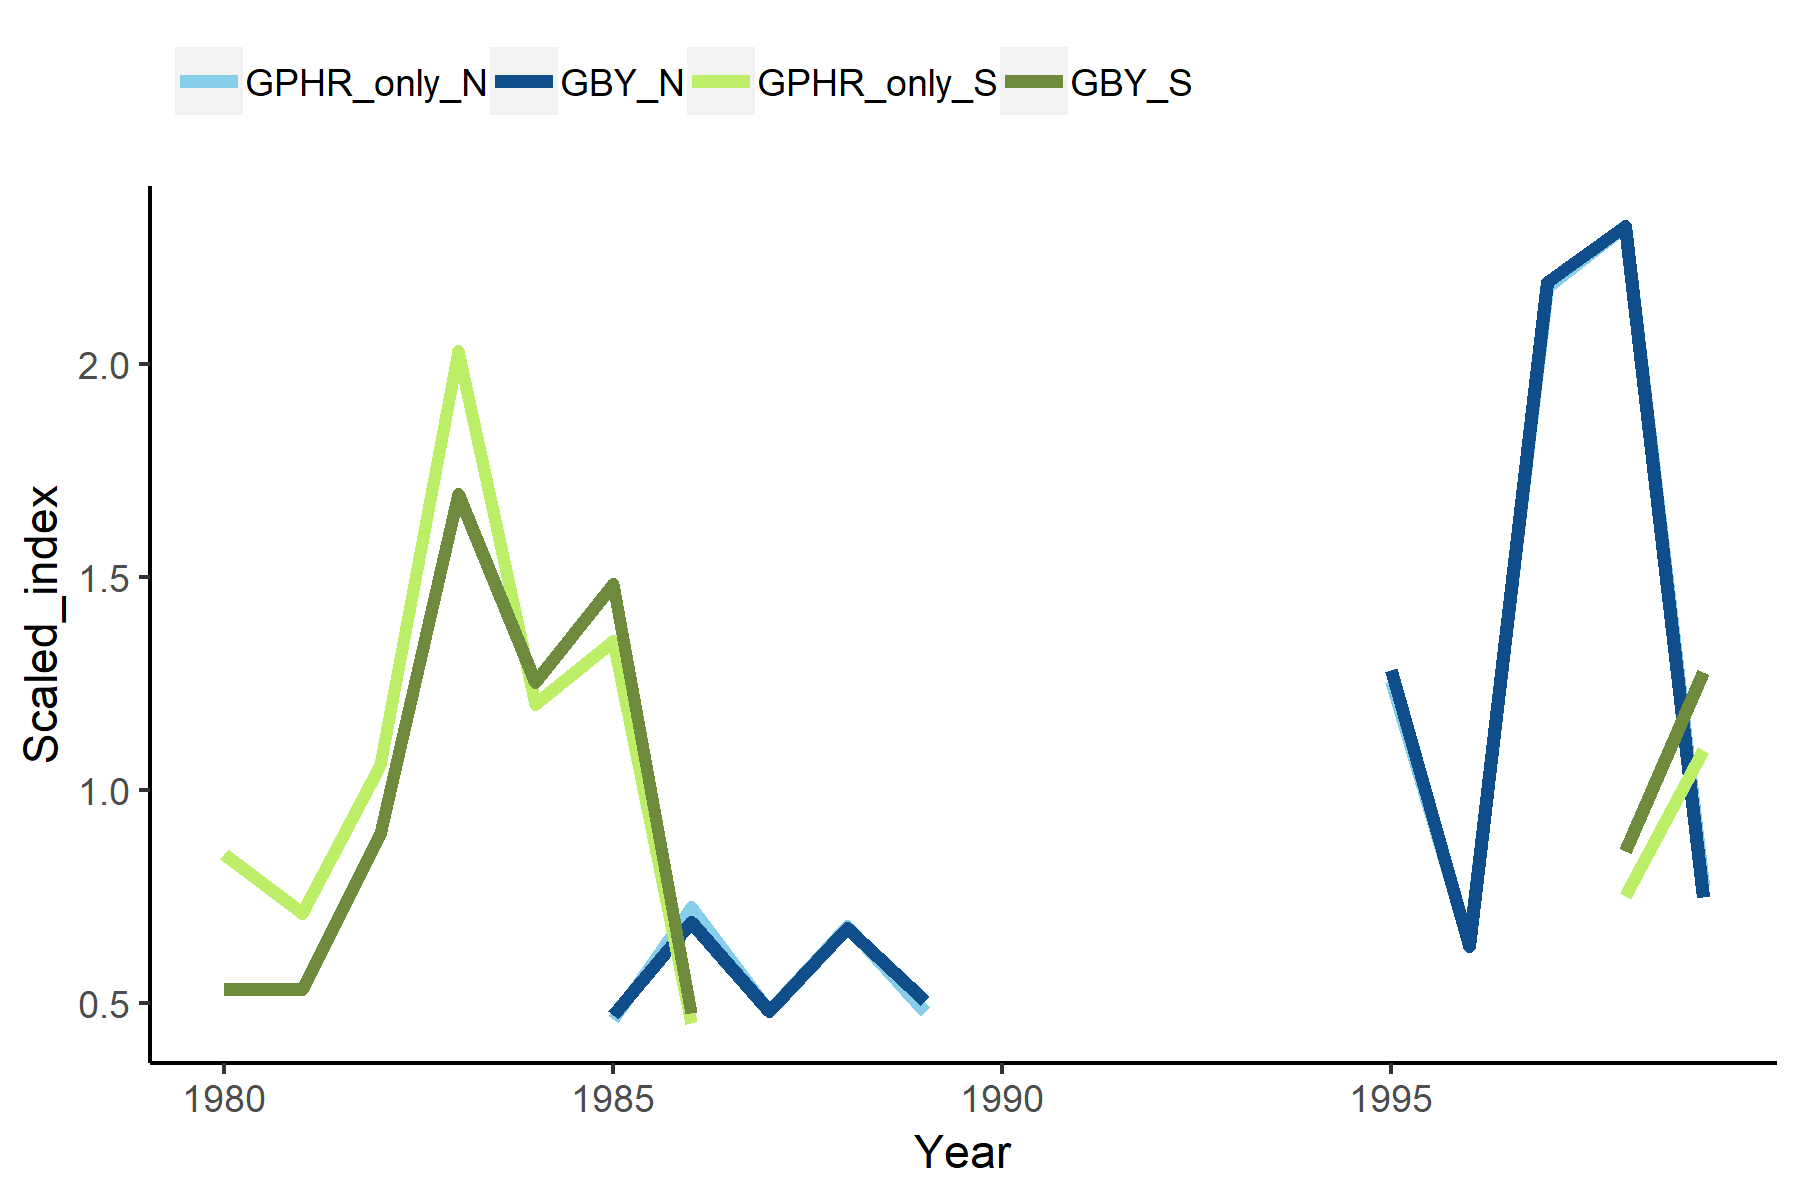
\includegraphics{Figures/MRFSS_index_compare.png}
\caption{Comparison of indices of abundance (scaled to their means) for
the MRFSS dockside CPFV survey between a gopher-only and GBYR complex
index for north and south of Point Conception.
\label{fig:MRFSS_index_compare}}
\end{figure}

\begin{figure}
\centering
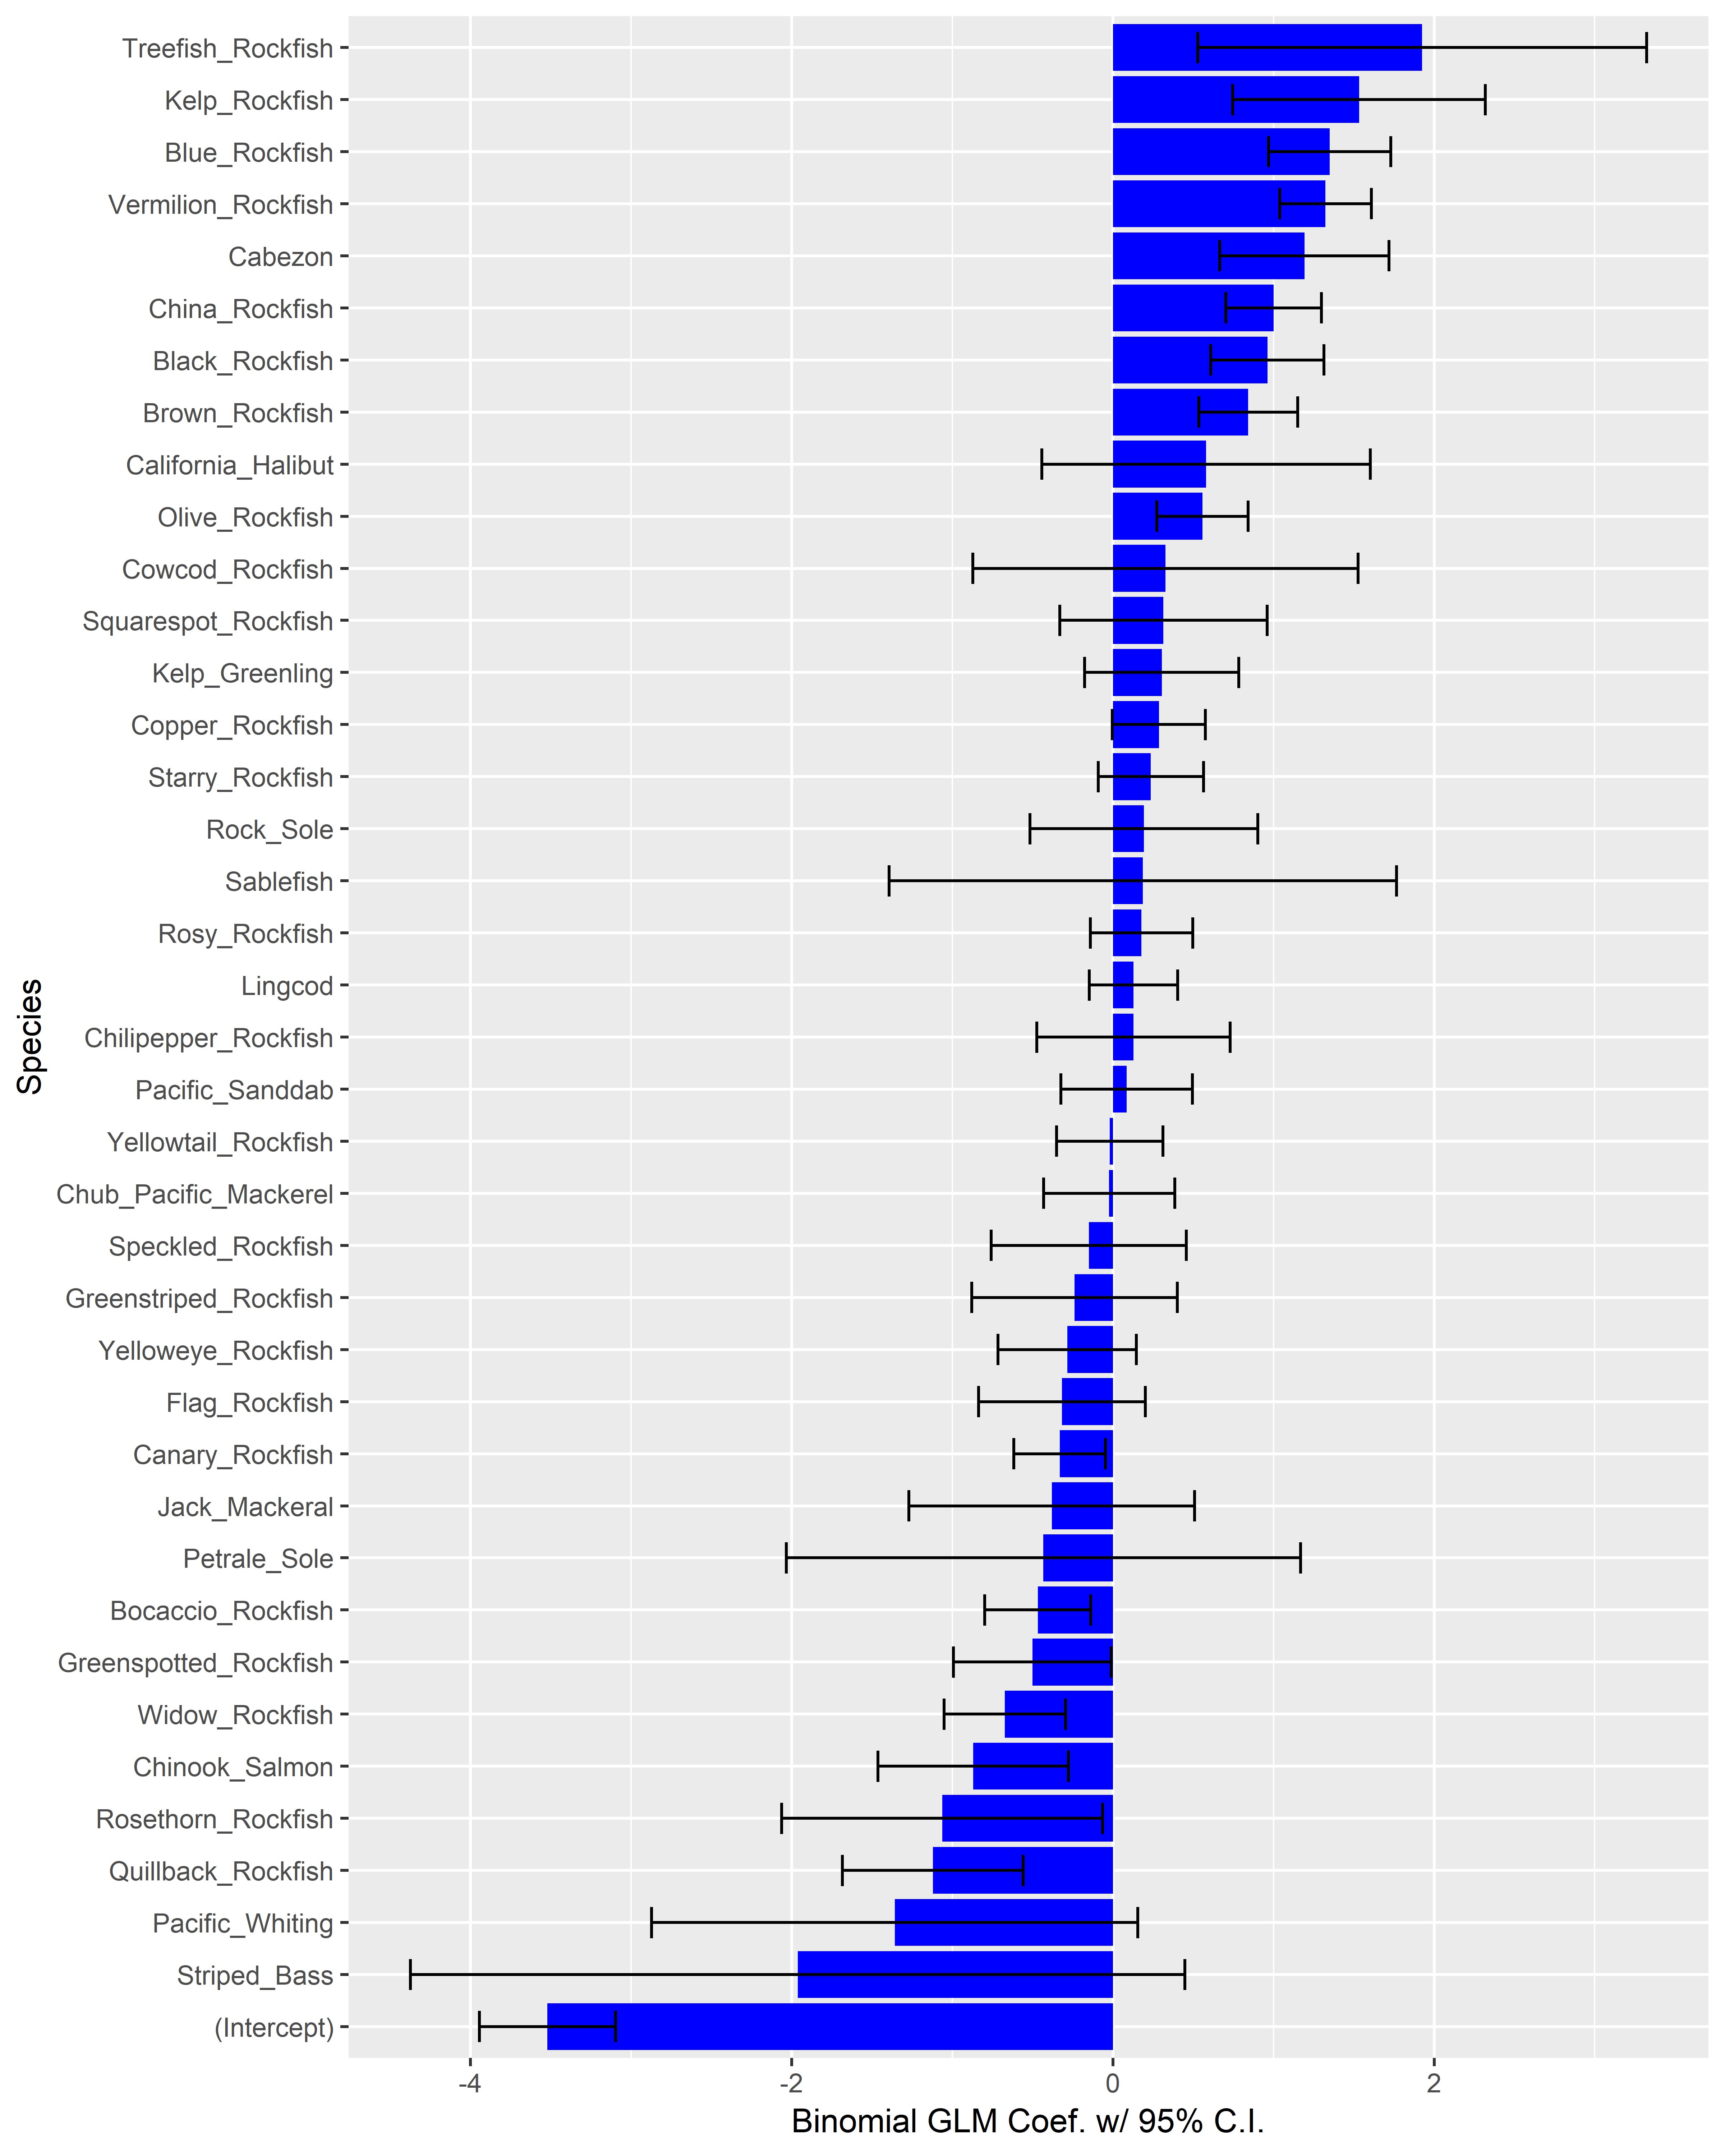
\includegraphics{Figures/Fleet10_SM_filter.png}
\caption{Species coefficients from the binomial GLM for presence/absence
of GBYR in the Marine Recreational Fisheries Statistics Survey (MRFSS)
CPFV mode dockside survey data set north of Point Conception. Horizontal
bars are 95\% confidence intervals. \label{fig:Fleet10_SM_filter}}
\end{figure}

\begin{figure}
\centering

\includegraphics{Figures/MRFSS_index_N_SM_falsepos.png}
\caption{Comparisons of the indices of abundance for GBYR north of Point
Conception from the MRFSS dockside CPFV survey that either include of
exclude the trips identified as false positives from the
Stephens-MacCall filter. \label{fig:MRFSS_index_N_SM_falsepos}}
\end{figure}

\begin{figure}
\centering
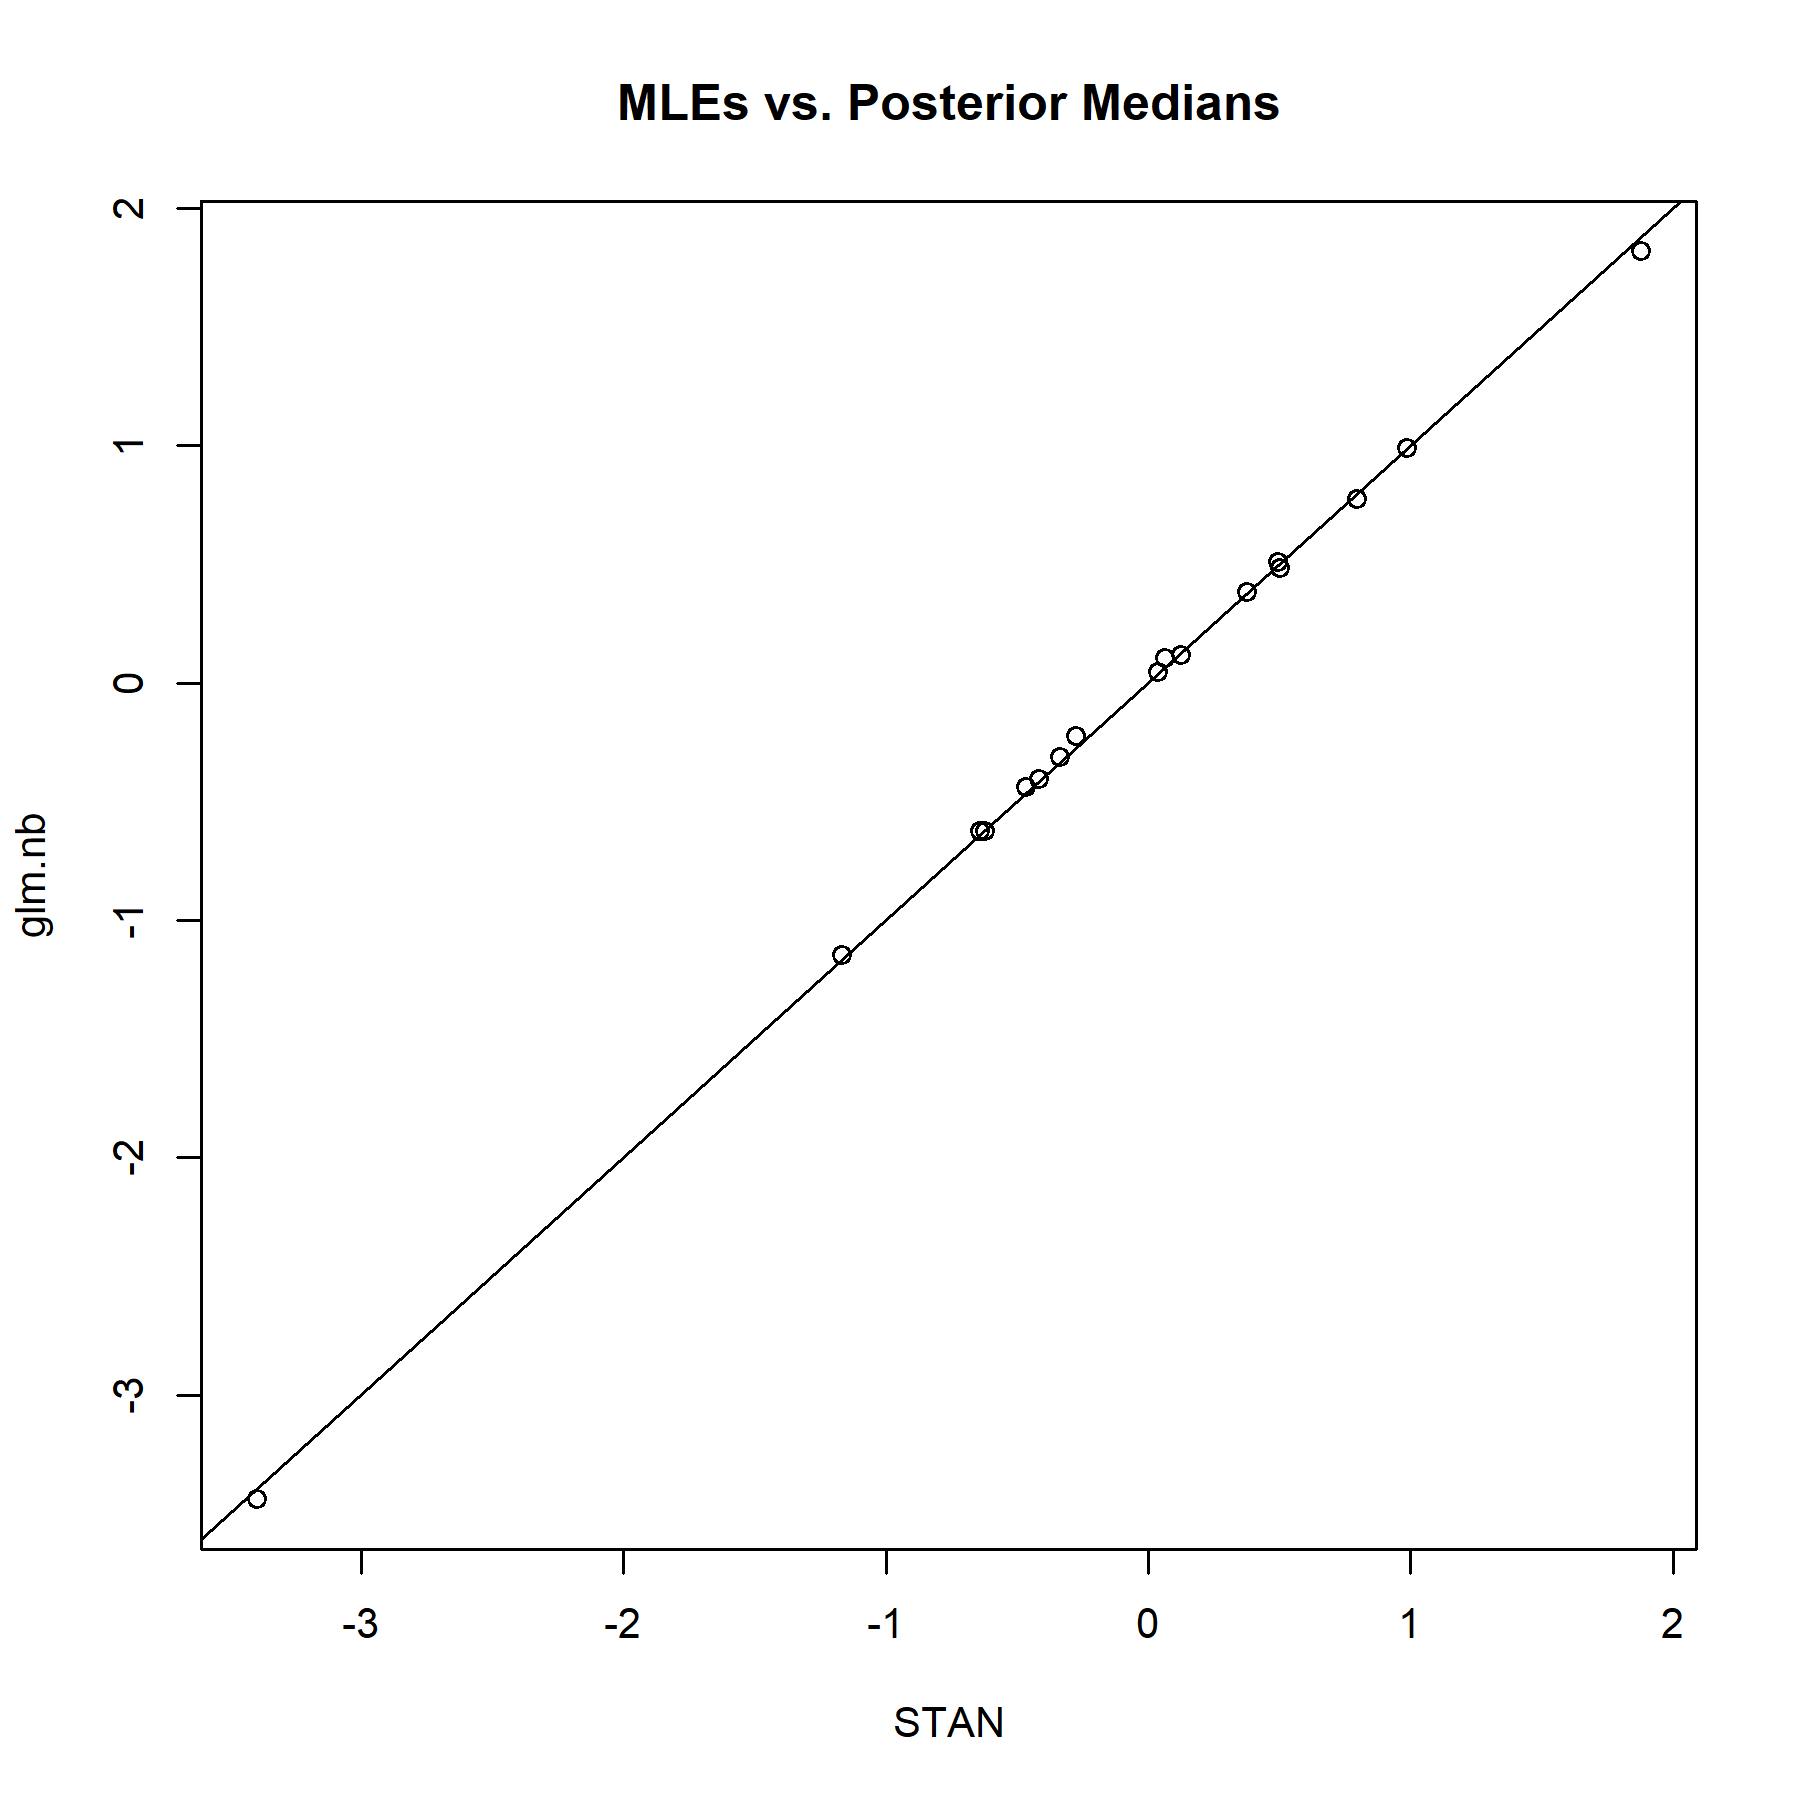
\includegraphics{Figures/Fleet10_MLE_stan.png}
\caption{Comparison of negative binomial predictions (CPUE) to observed
means in each stratum (year) MRFSS CPFV dockside index north of Point
Conception. The 1:1 plot is for reference. \label{fig:Fleet10_MLE_stan}}
\end{figure}

\begin{figure}
\centering
\includegraphics{Figures/Fleet10_prop_zero_STAN.png}
\caption{Posterior predictive distribution of the proportion of zero
observations in replicate data sets generated by the negative binomial
model for MRFSS dockside CPFV index north of Point Conception.
\label{fig:Fleet10_prop_zero_STAN}}
\end{figure}

\FloatBarrier

\begin{figure}
\centering
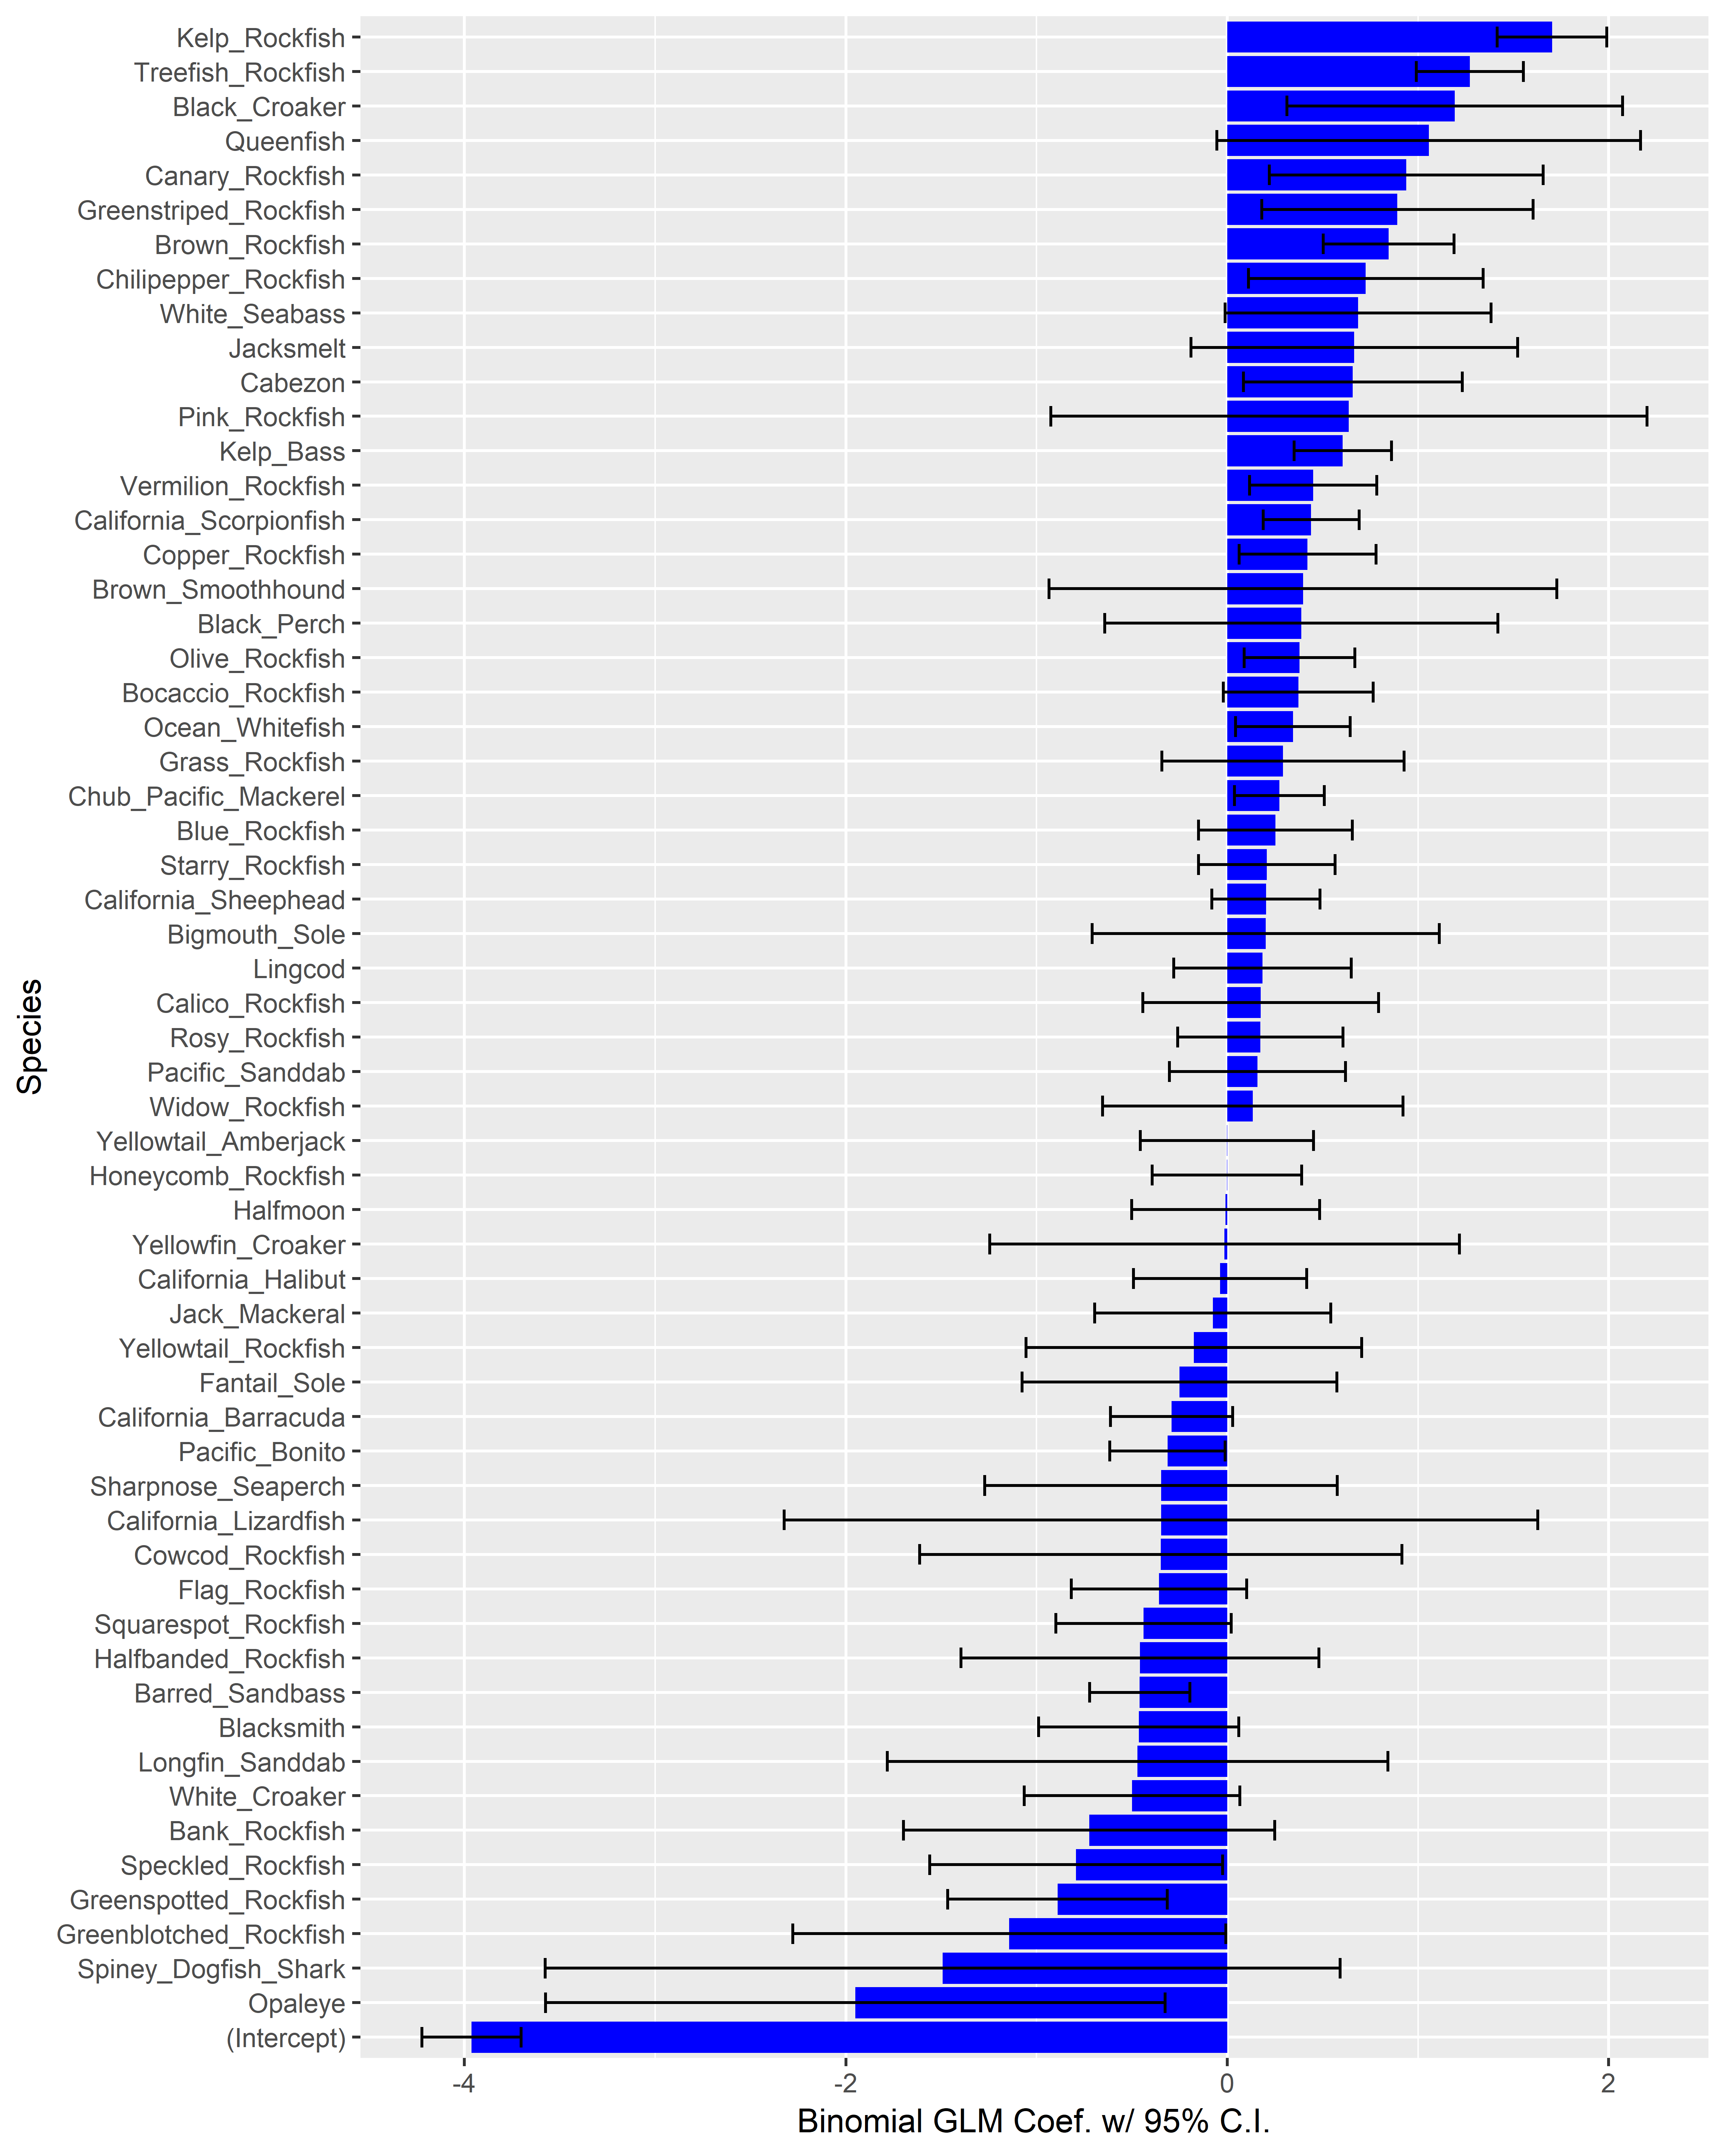
\includegraphics{Figures/Fleet11_SM_filter.png}
\caption{Species coefficients from the binomial GLM for presence/absence
of GBYR in the Marine Recreational Fisheries Statistics Survey (MRFSS)
CPFV mode dockside survey data set north of Point Conception. Horizontal
bars are 95\% confidence intervals. \label{fig:Fleet11_SM_filter}}
\end{figure}

\FloatBarrier

\begin{figure}
\centering
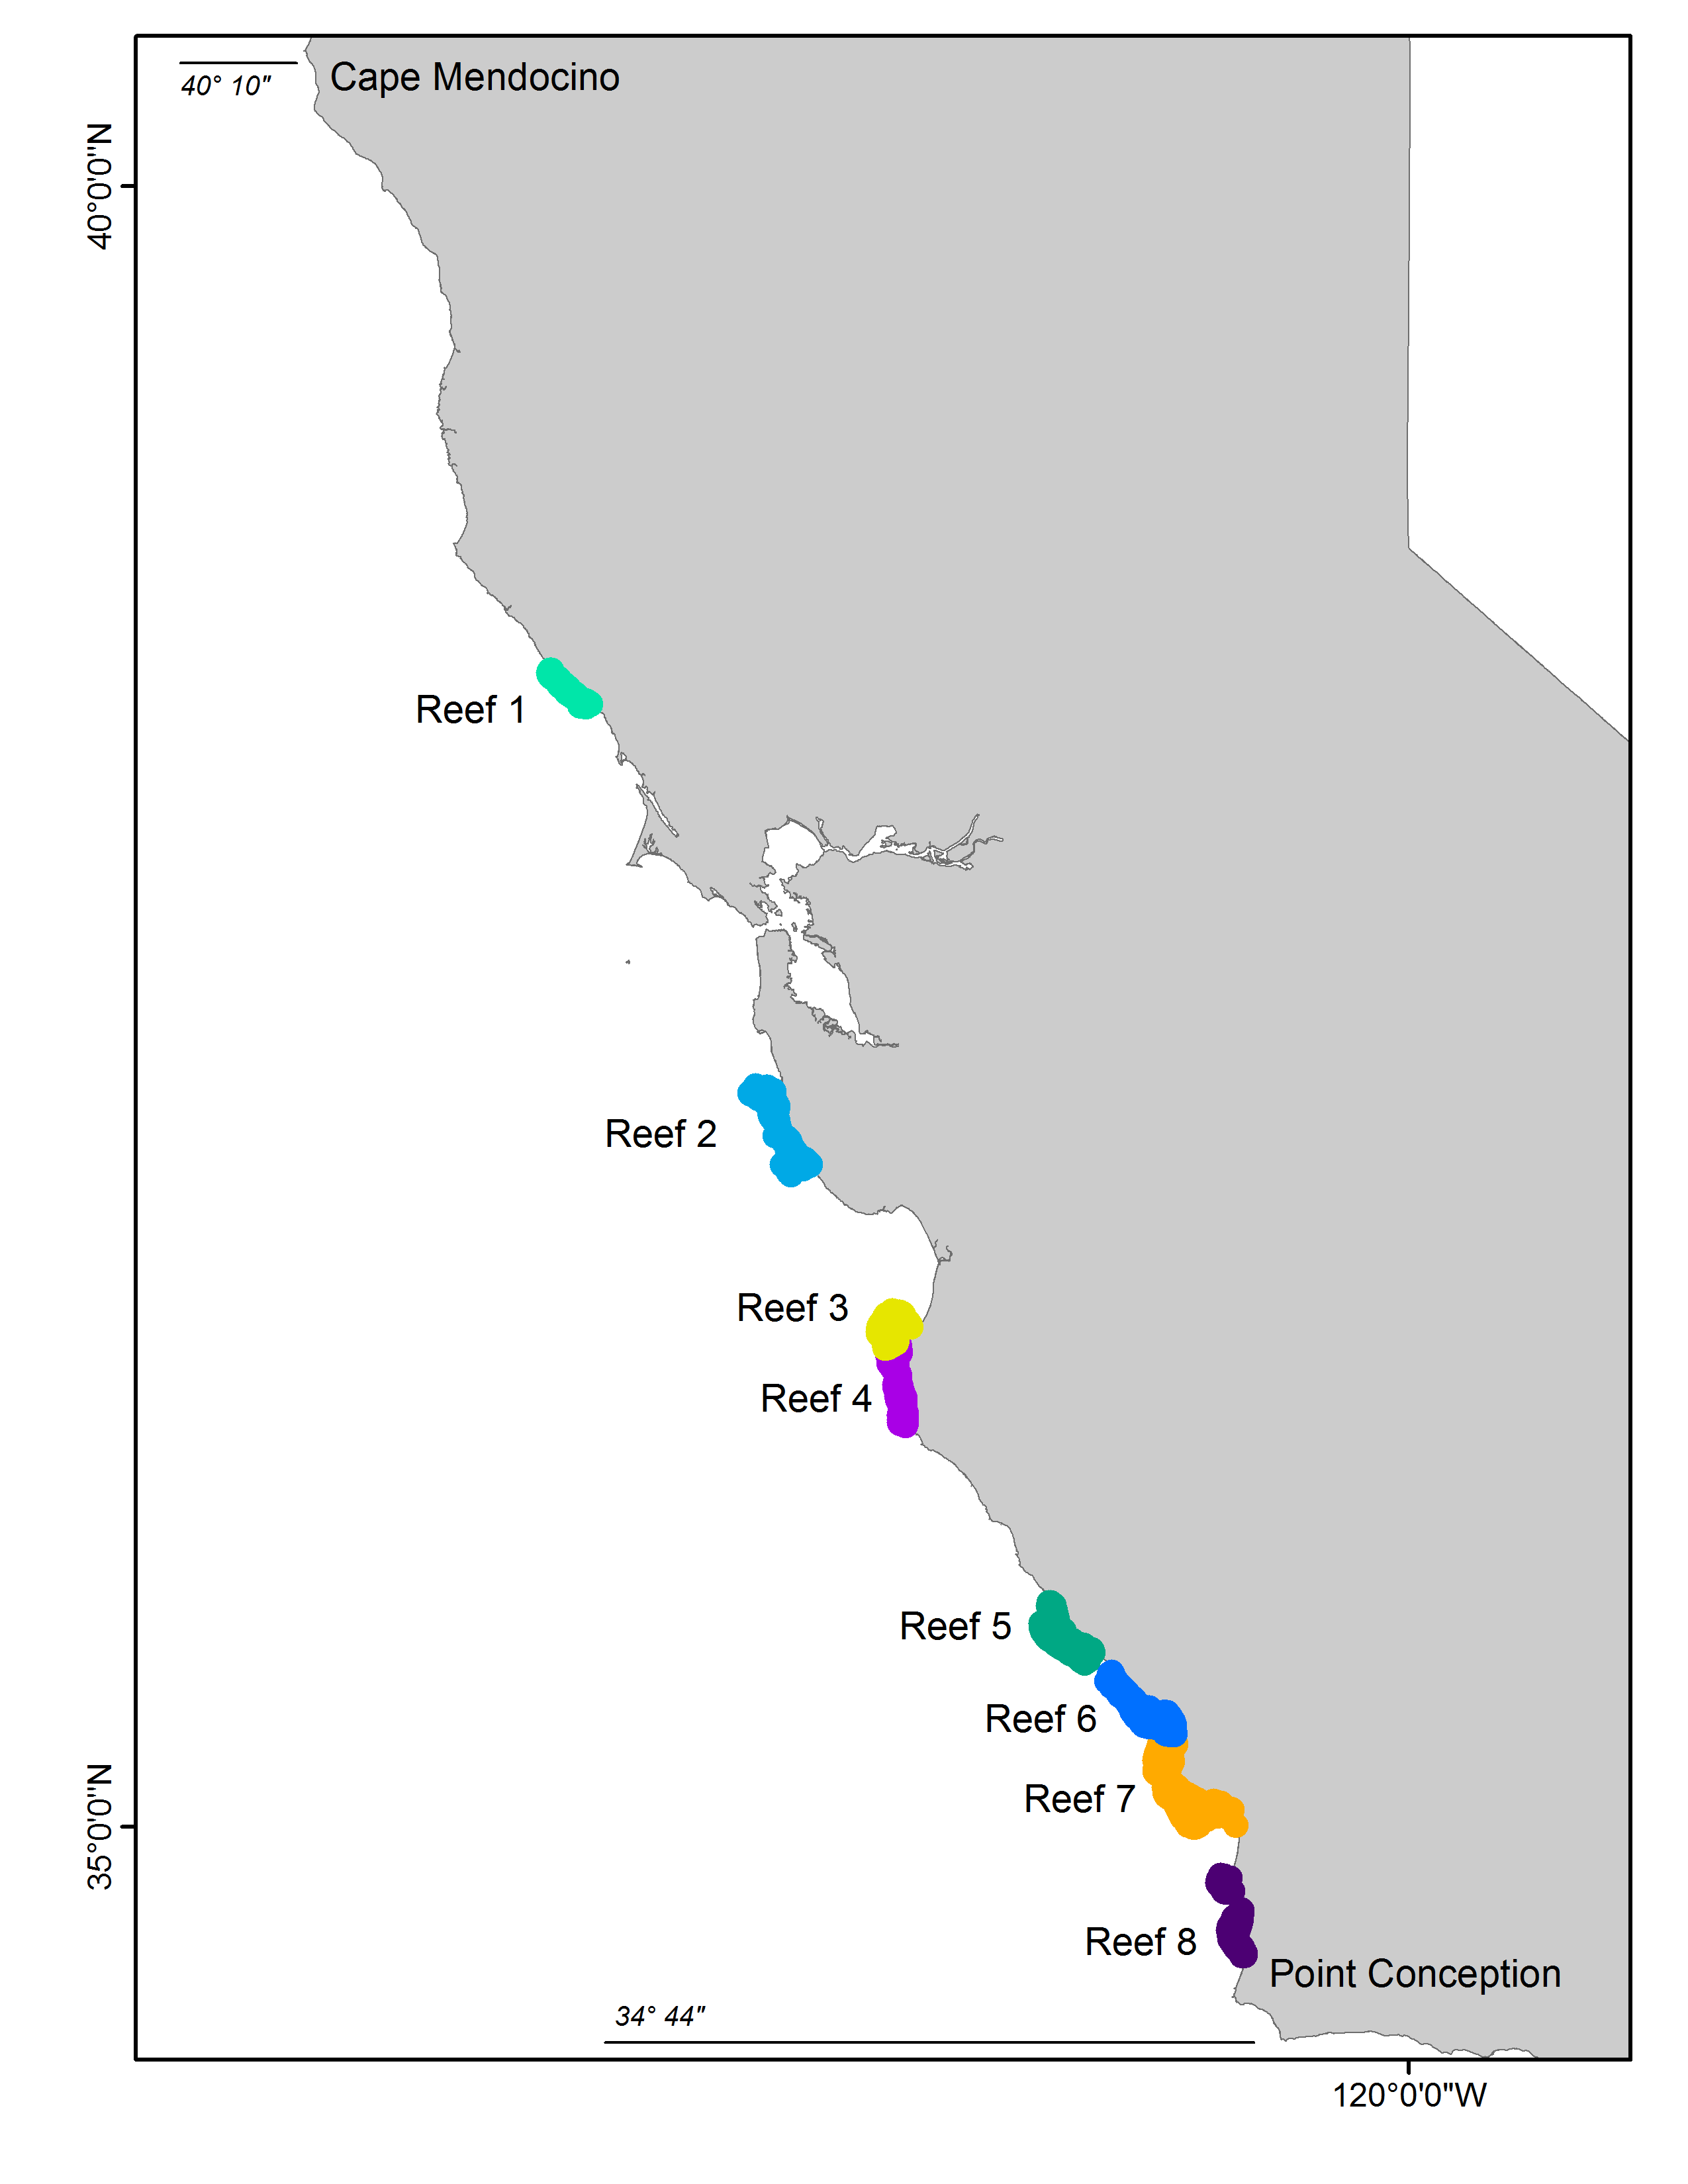
\includegraphics{Figures/DebWV_sites.png}
\caption{Map of the reefs used in the Deb Wilson-Vandenberg CPFV onboard
observer survey index of abundance. \label{fig:DebWV_sites}}
\end{figure}

\begin{figure}
\centering
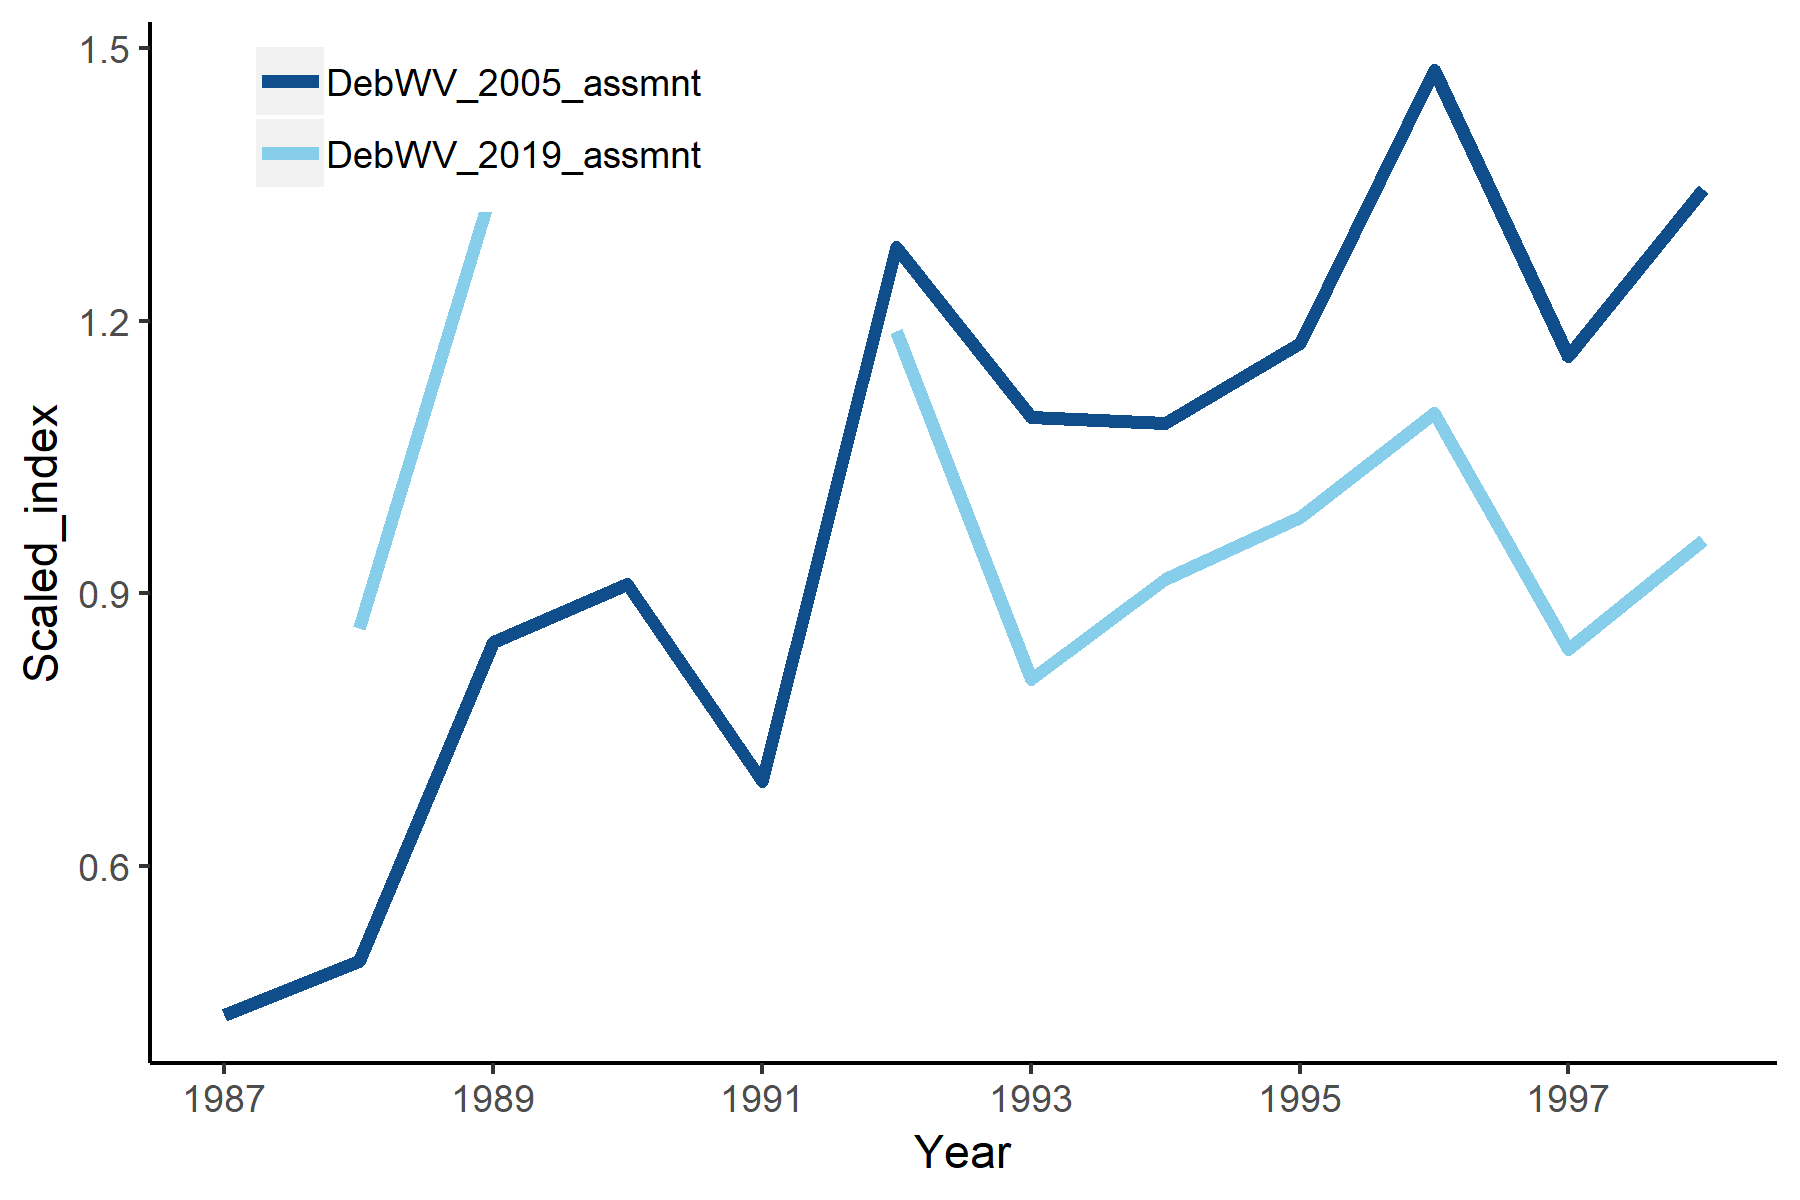
\includegraphics{Figures/DebWV_index_compare.png}
\caption{Comparison of the index developed for the Deb Wilson-Vandenberg
CPFV onboard observer survey from the 2005 assessment and for the 2019
assessment. \label{fig:DebWV_index_compare}}
\end{figure}

\FloatBarrier

\begin{figure}
\centering
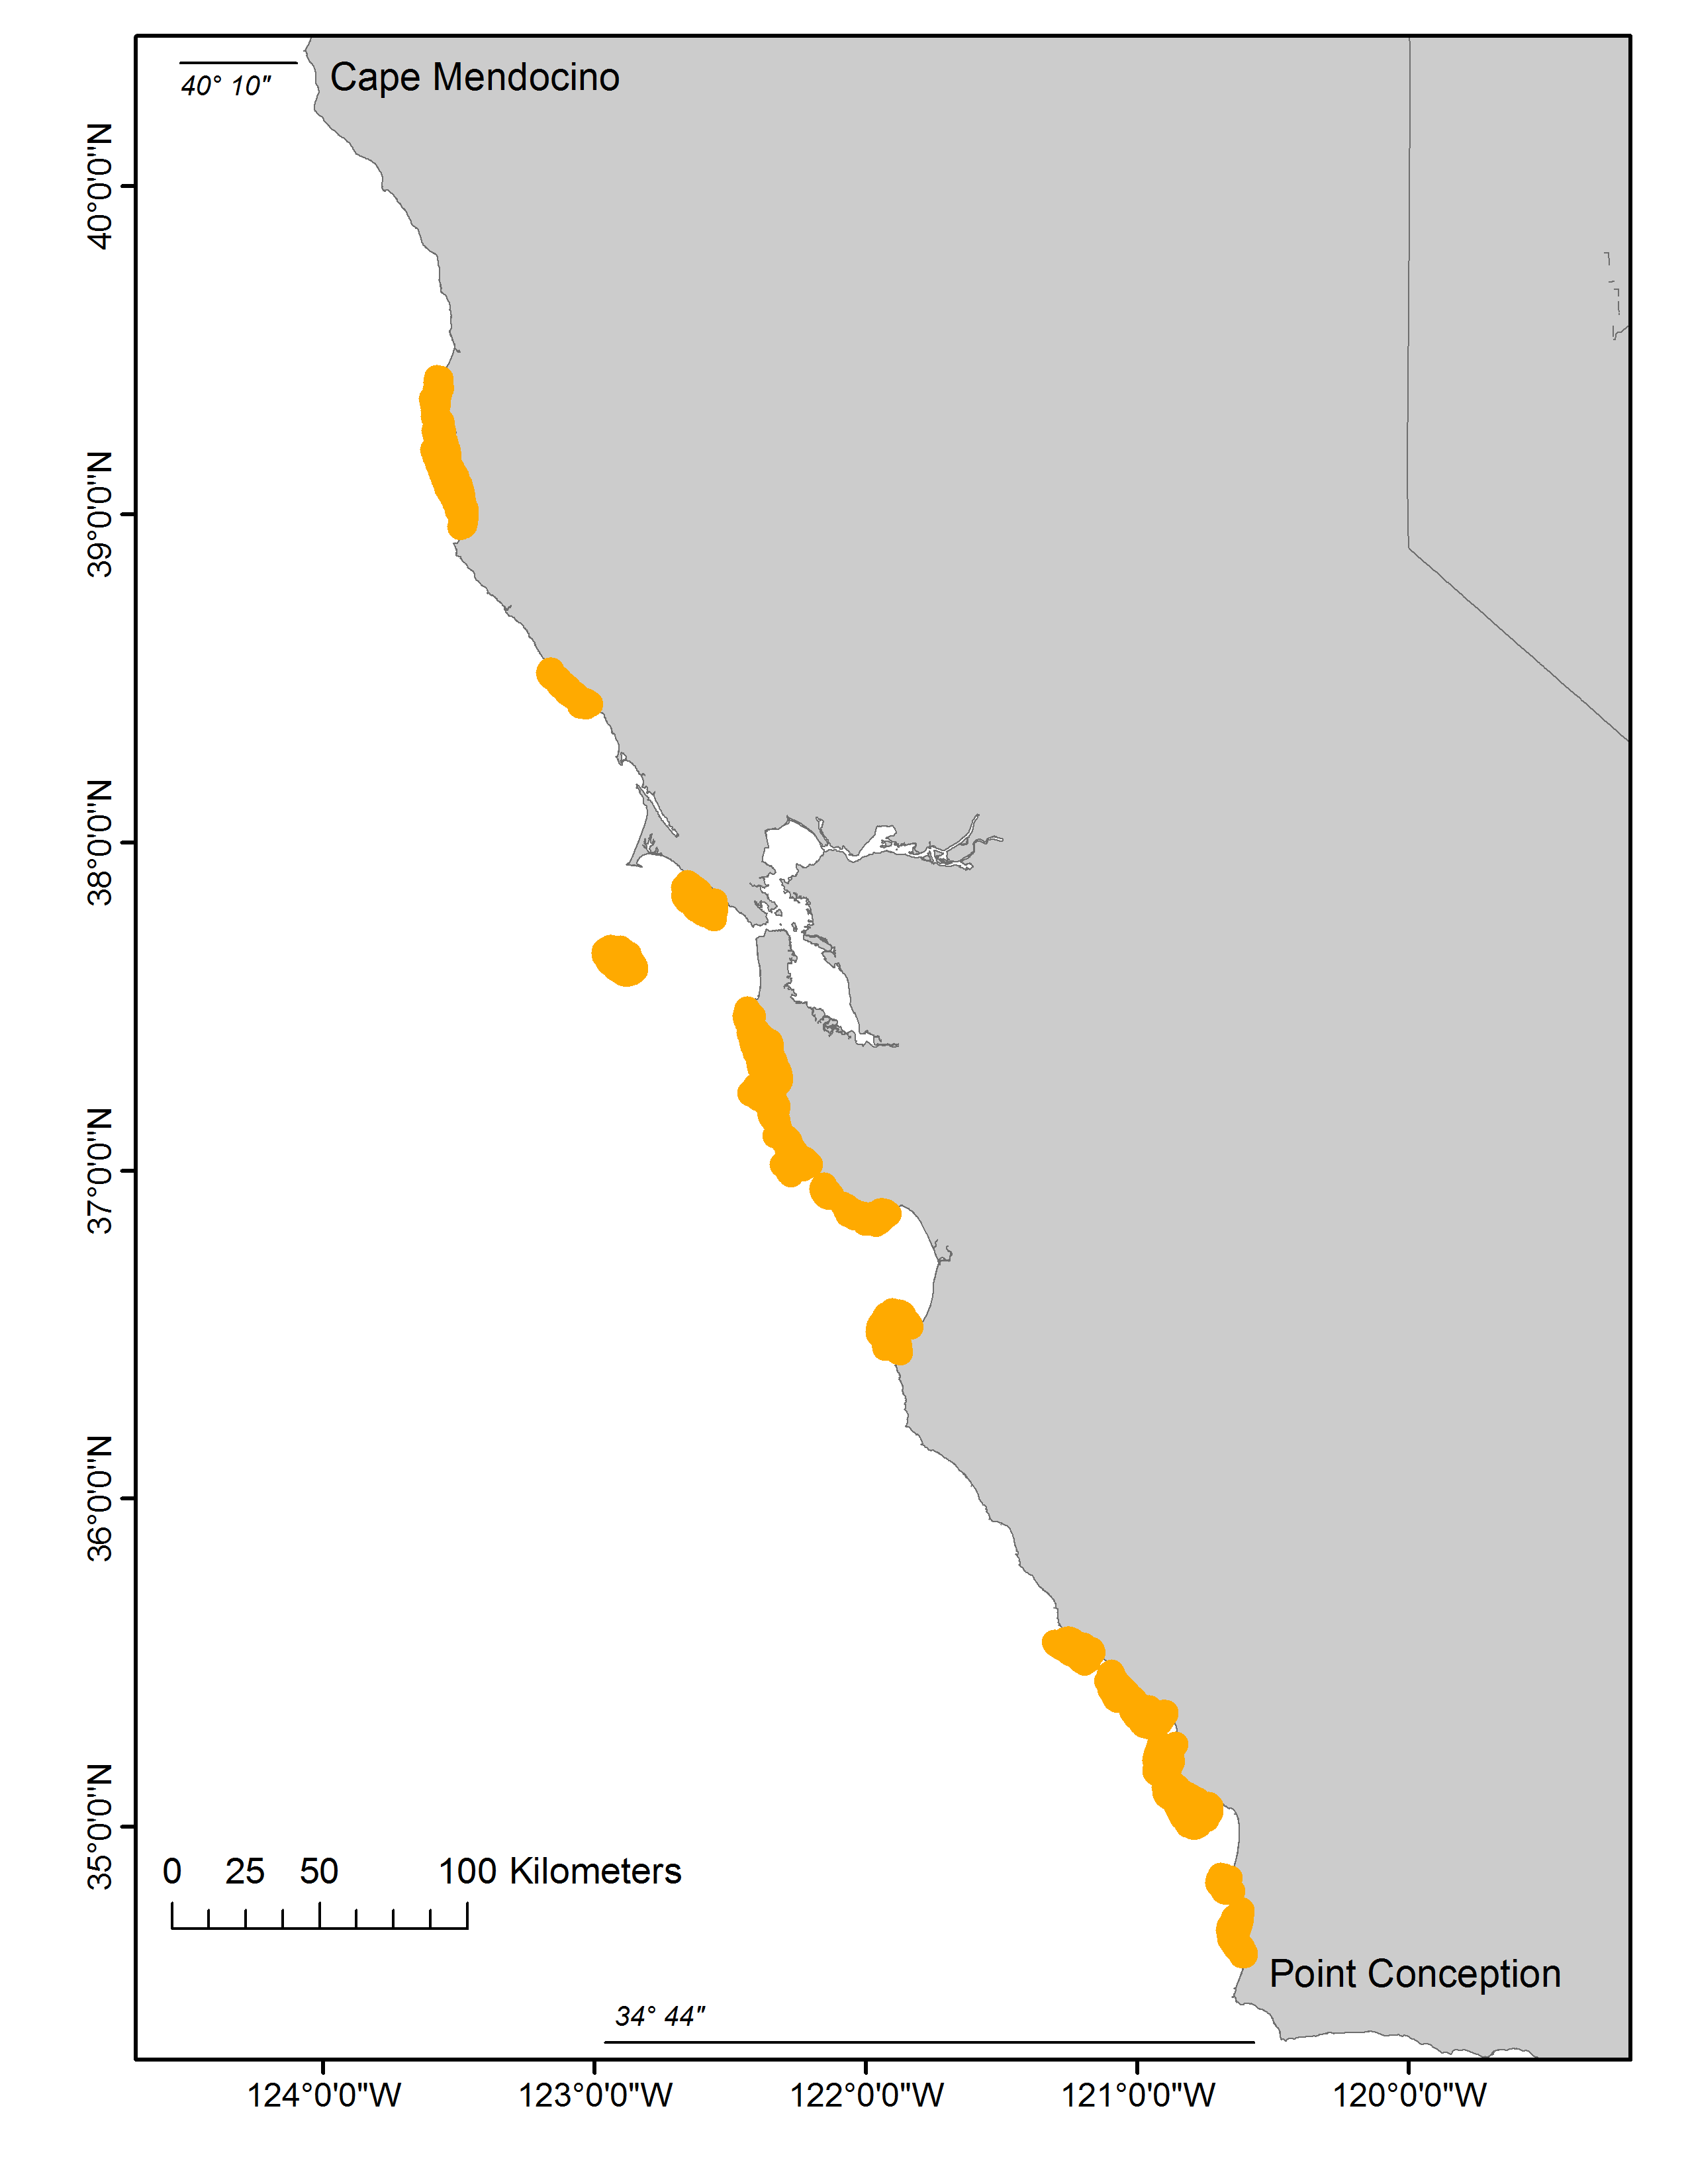
\includegraphics{Figures/Onboard_observer_north_sites.png}
\caption{Map of the reefs selected for the final index for the onboard
observer surveys (CDFW and Cal Poly) north of Point Conception
\label{fig:Onboard_observer_north_sites}}
\end{figure}

\FloatBarrier

\begin{figure}
\centering
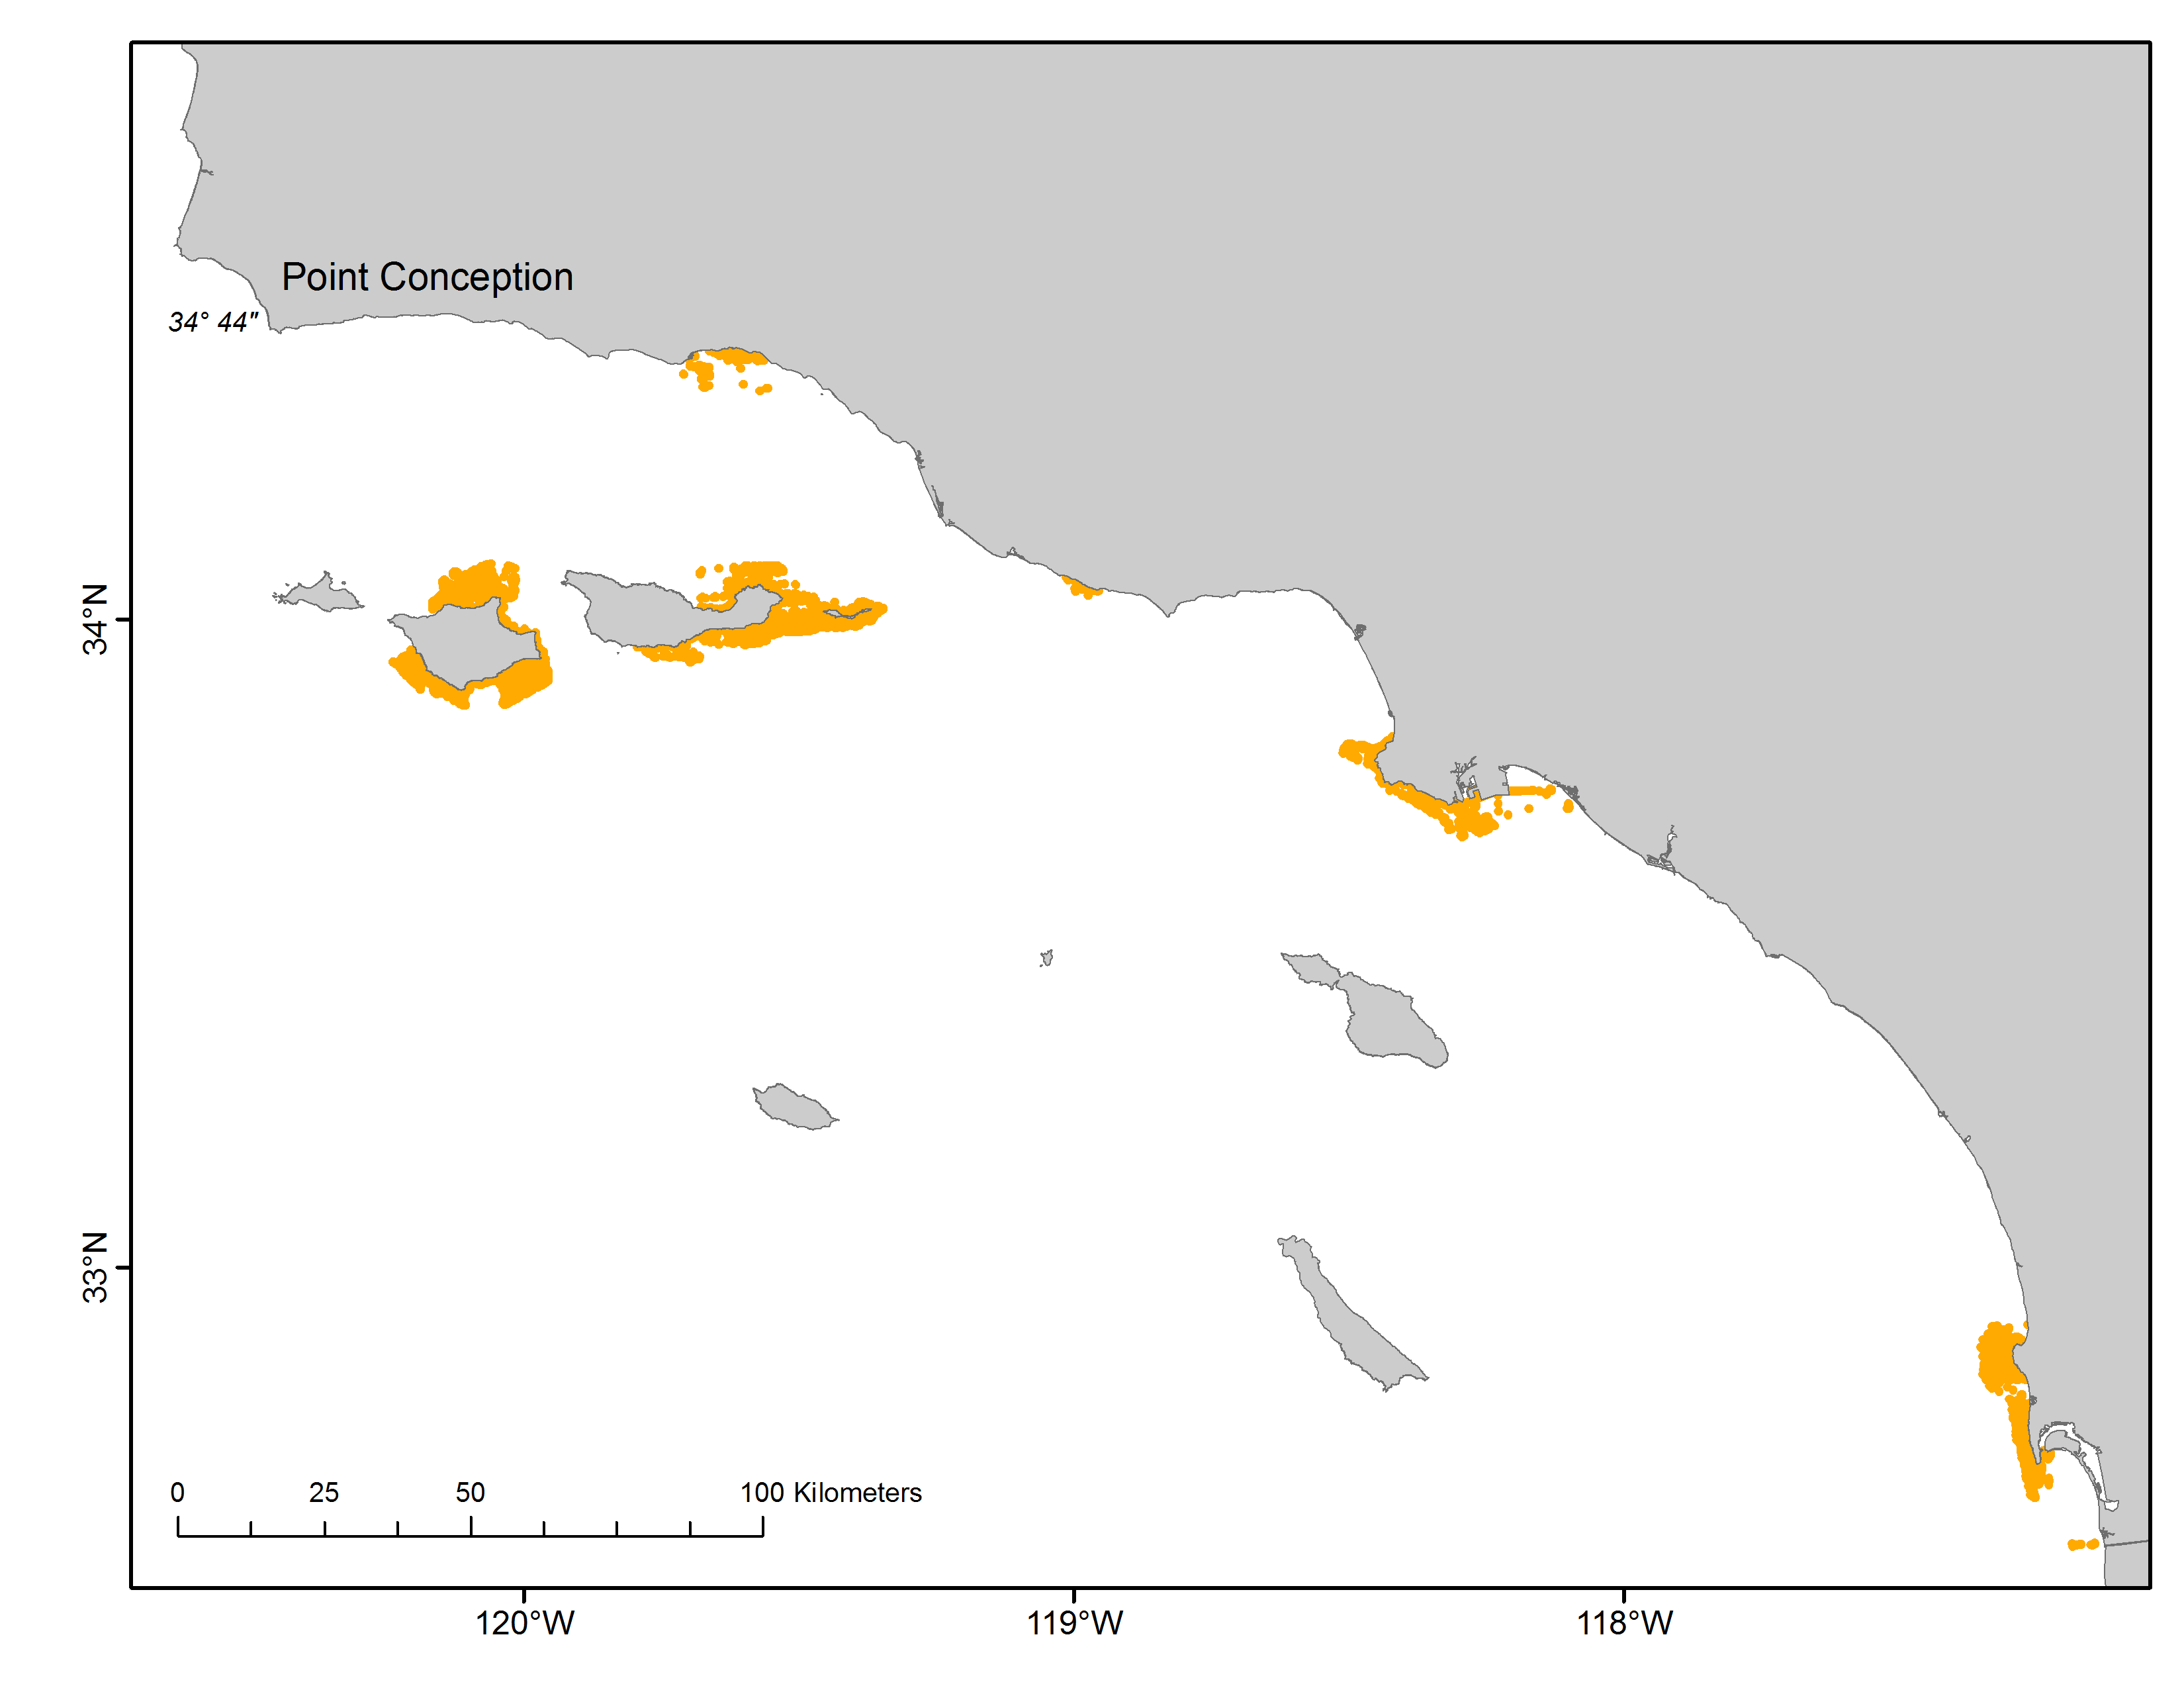
\includegraphics{Figures/Onboard_observer_south_sites.png}
\caption{Map of the reefs selected for the final index for the CDFW
onboard observer survey south of Point Conception
\label{fig:Onboard_observer_south_sites}}
\end{figure}

\FloatBarrier 

\begin{figure}
\centering
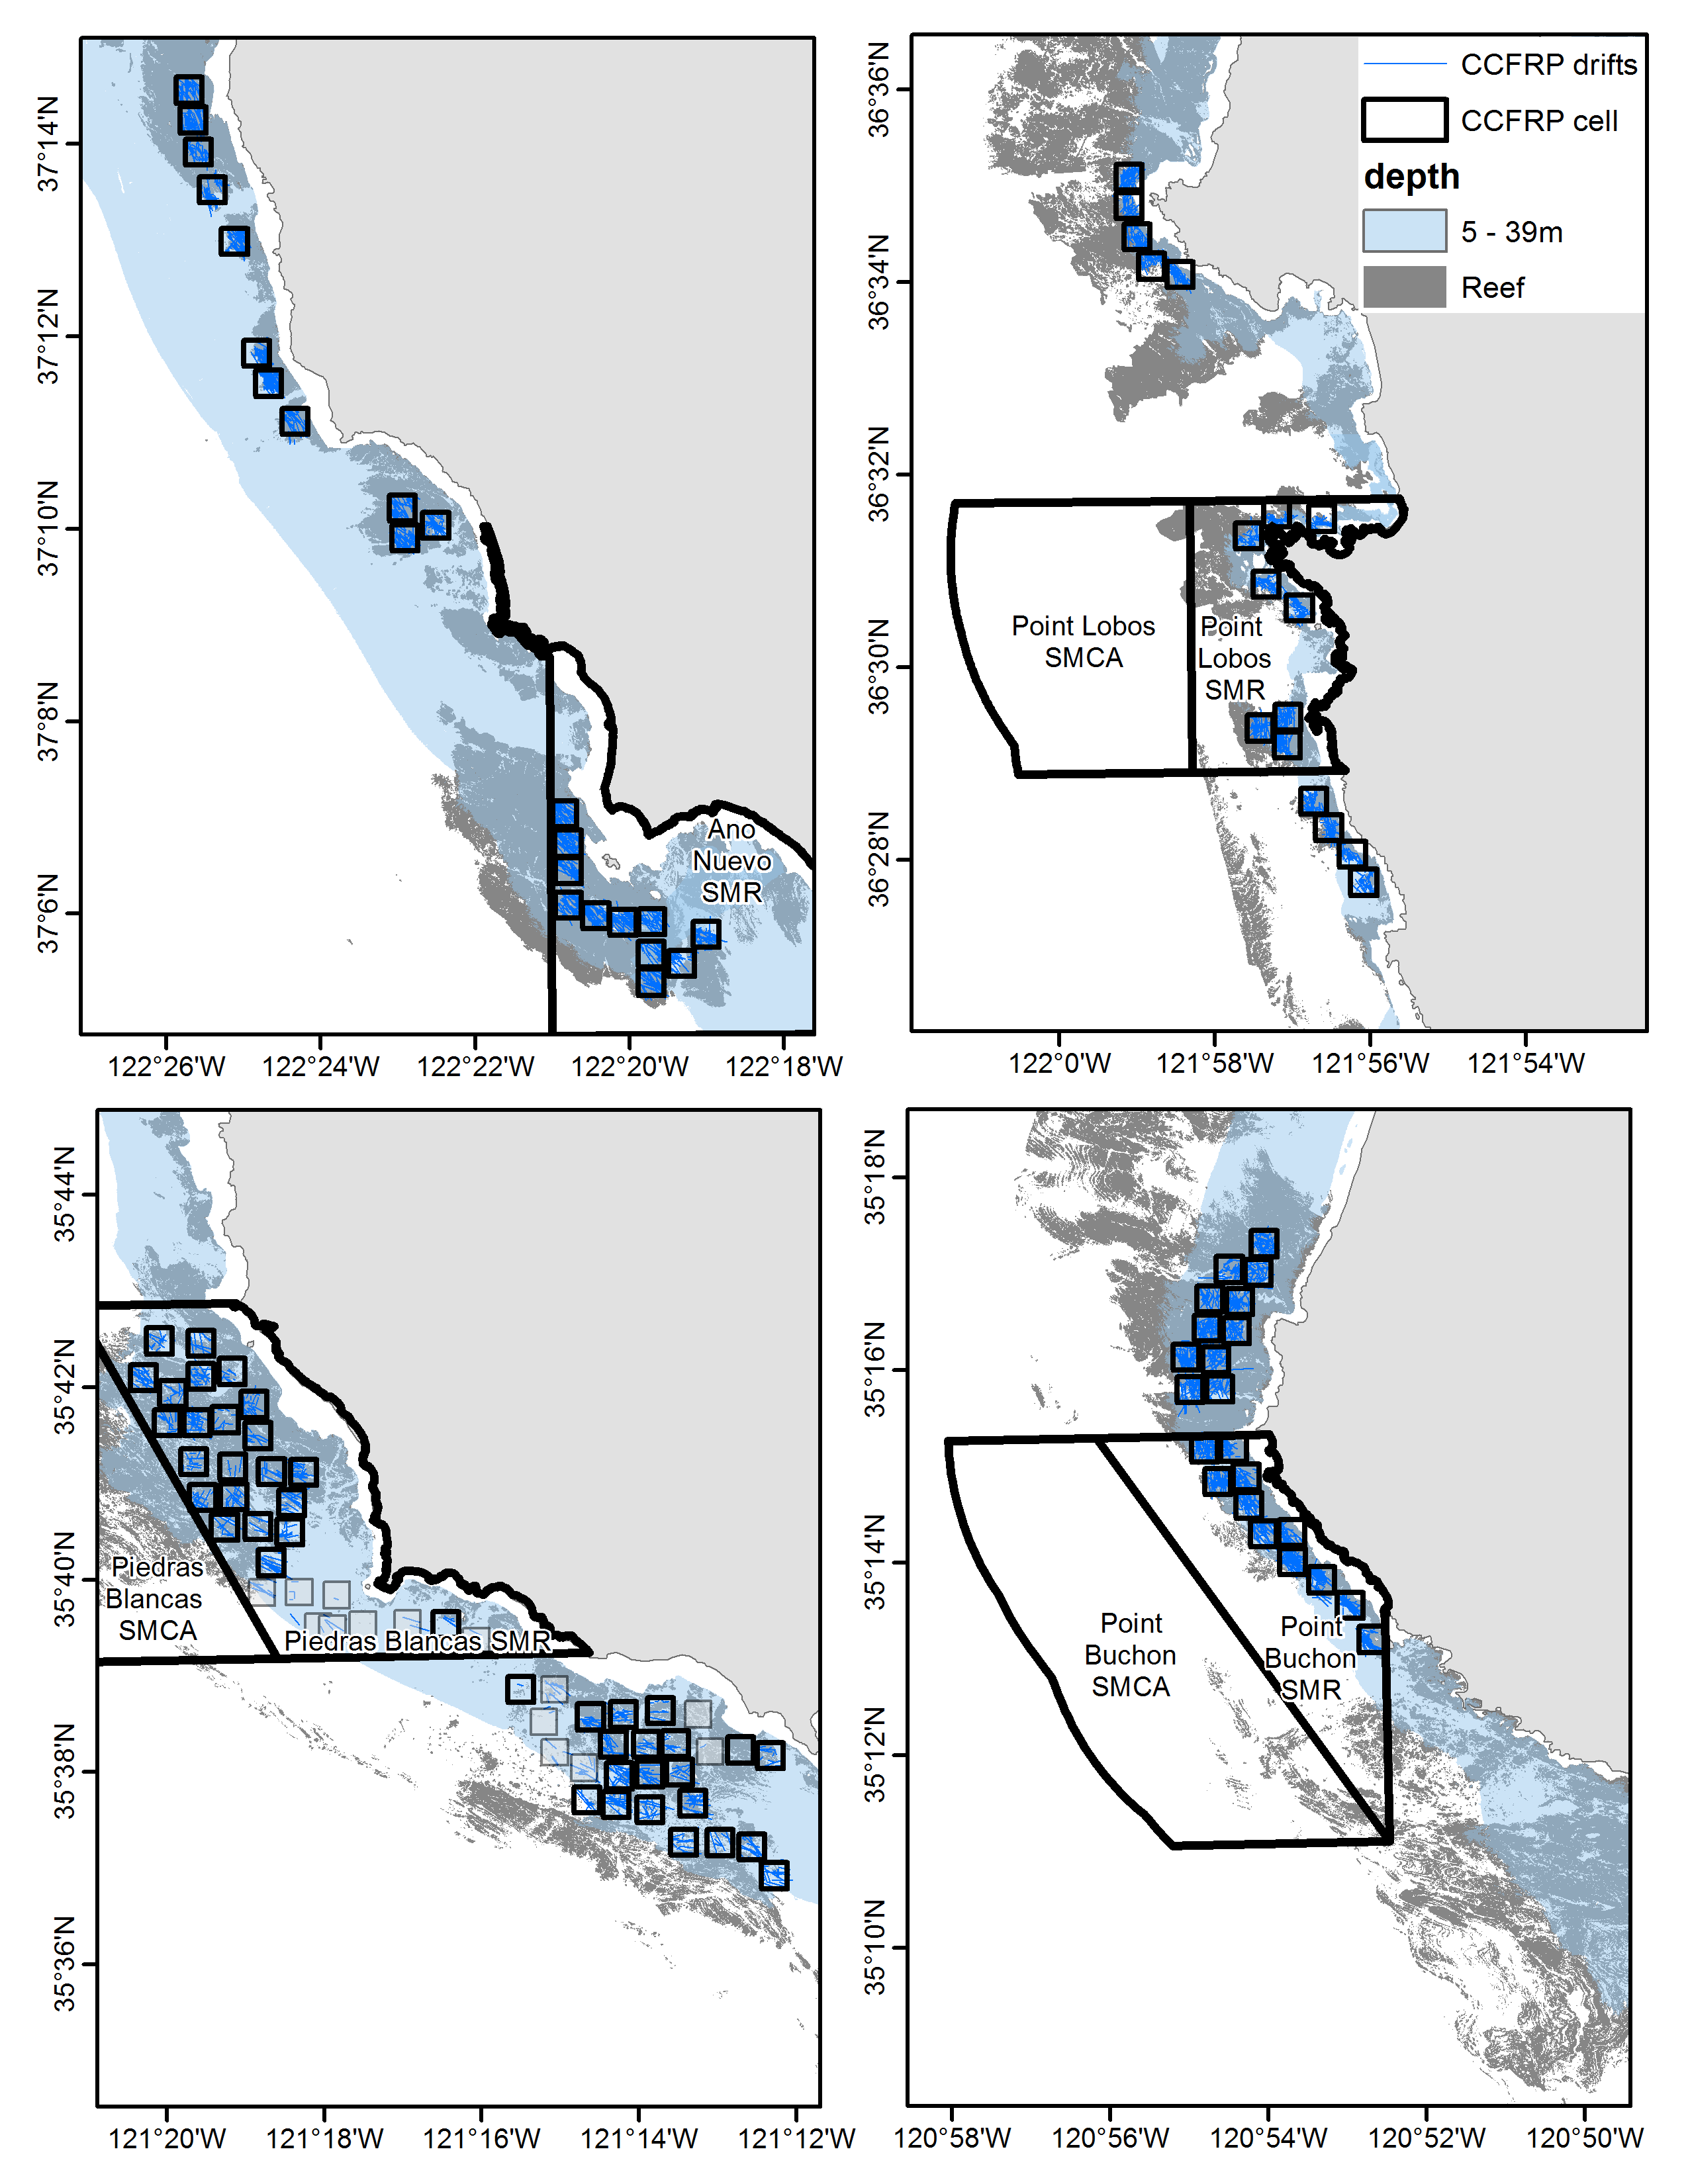
\includegraphics{Figures/CCFRP_sites.png}
\caption{Map of the four MPAs sampled consistently through time for the
CCFRP fishery-independent survey. \label{fig:CCFRP_sites}}
\end{figure}

\FloatBarrier

\begin{figure}
\centering
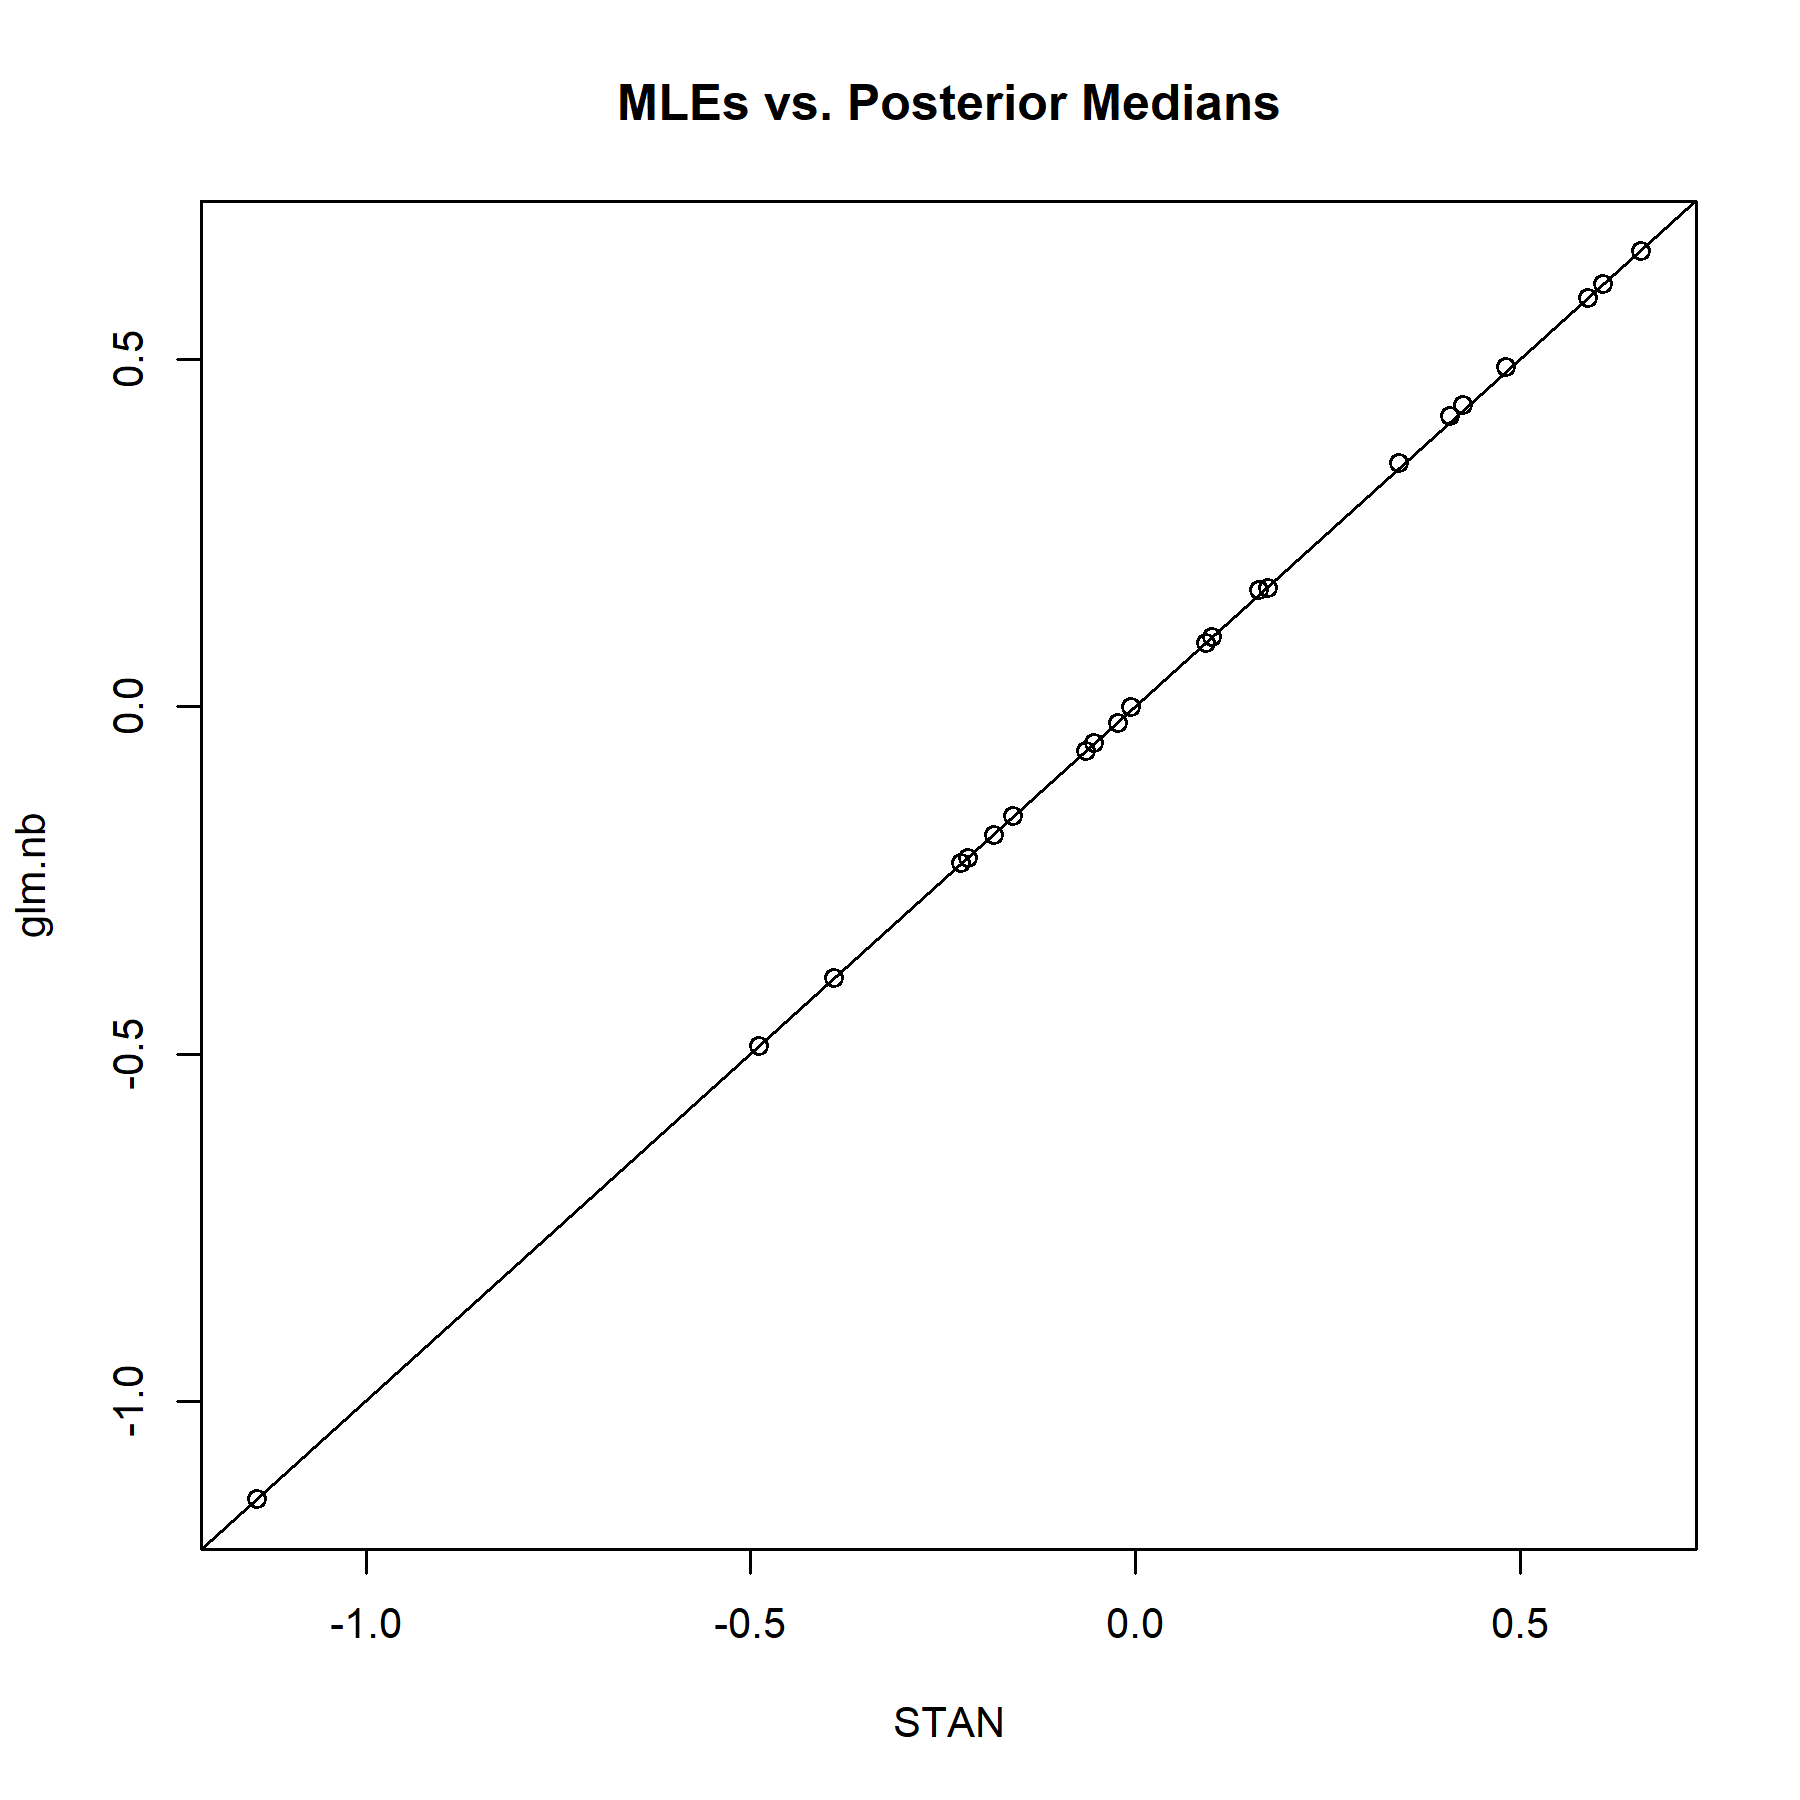
\includegraphics{Figures/Fleet9_MLE_stan.png}
\caption{Comparison of negative bionimial predictions (CPUE) to observed
means in each stratum (year) for the CCFRP index. The 1:1 plot is for
reference. \label{fig:Fleet9_MLE_stan}}
\end{figure}

\FloatBarrier

\begin{figure}
\centering
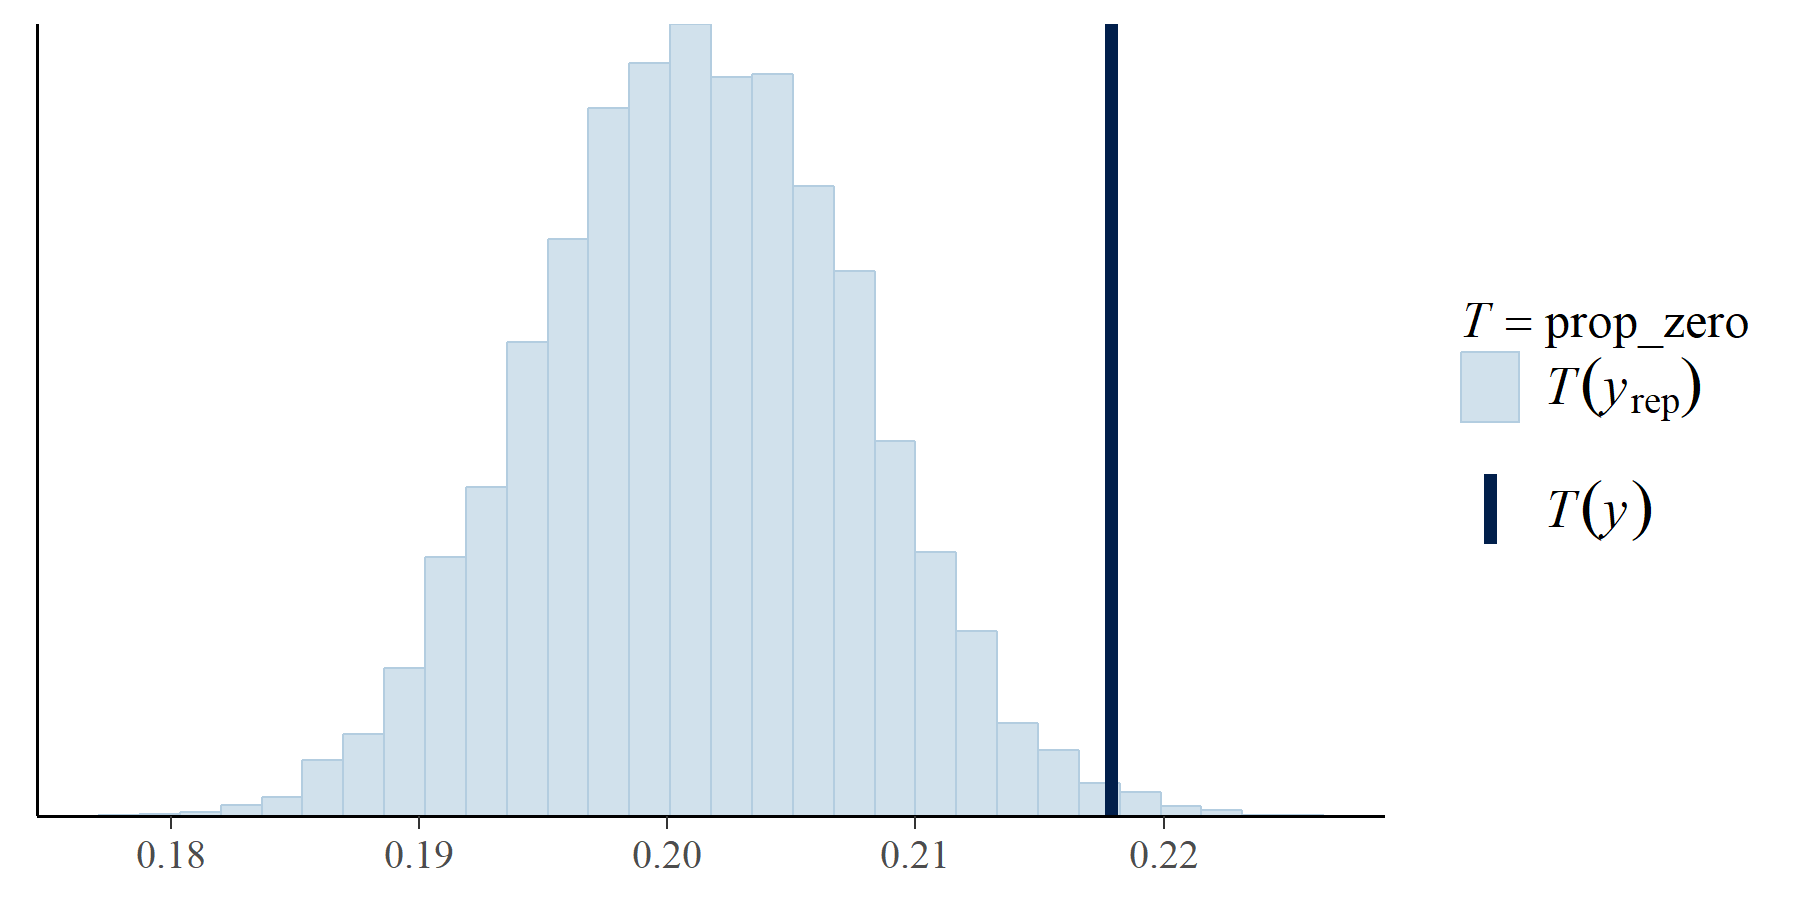
\includegraphics{Figures/Fleet9_prop_zero_STAN.png}
\caption{Posterior predictive distribution of the proportion of zero
observations in replicate data sets generated by the negative binomial
model for the CCFRP index. \label{fig:Fleet9_prop_zero_STAN}}
\end{figure}

\FloatBarrier

\begin{figure}
\centering
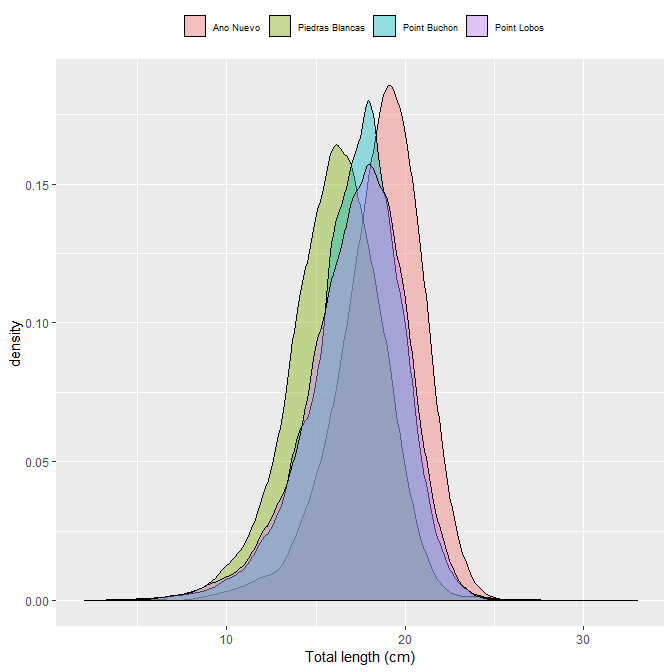
\includegraphics{Figures/CCFRP_lengths_by_site.png}
\caption{Length distributions of GBYR for the four MPAs sampled by the
CCFRP survey used in this assessment. \label{CCFRP_lengths_by_site}}
\end{figure}

\begin{figure}
\centering
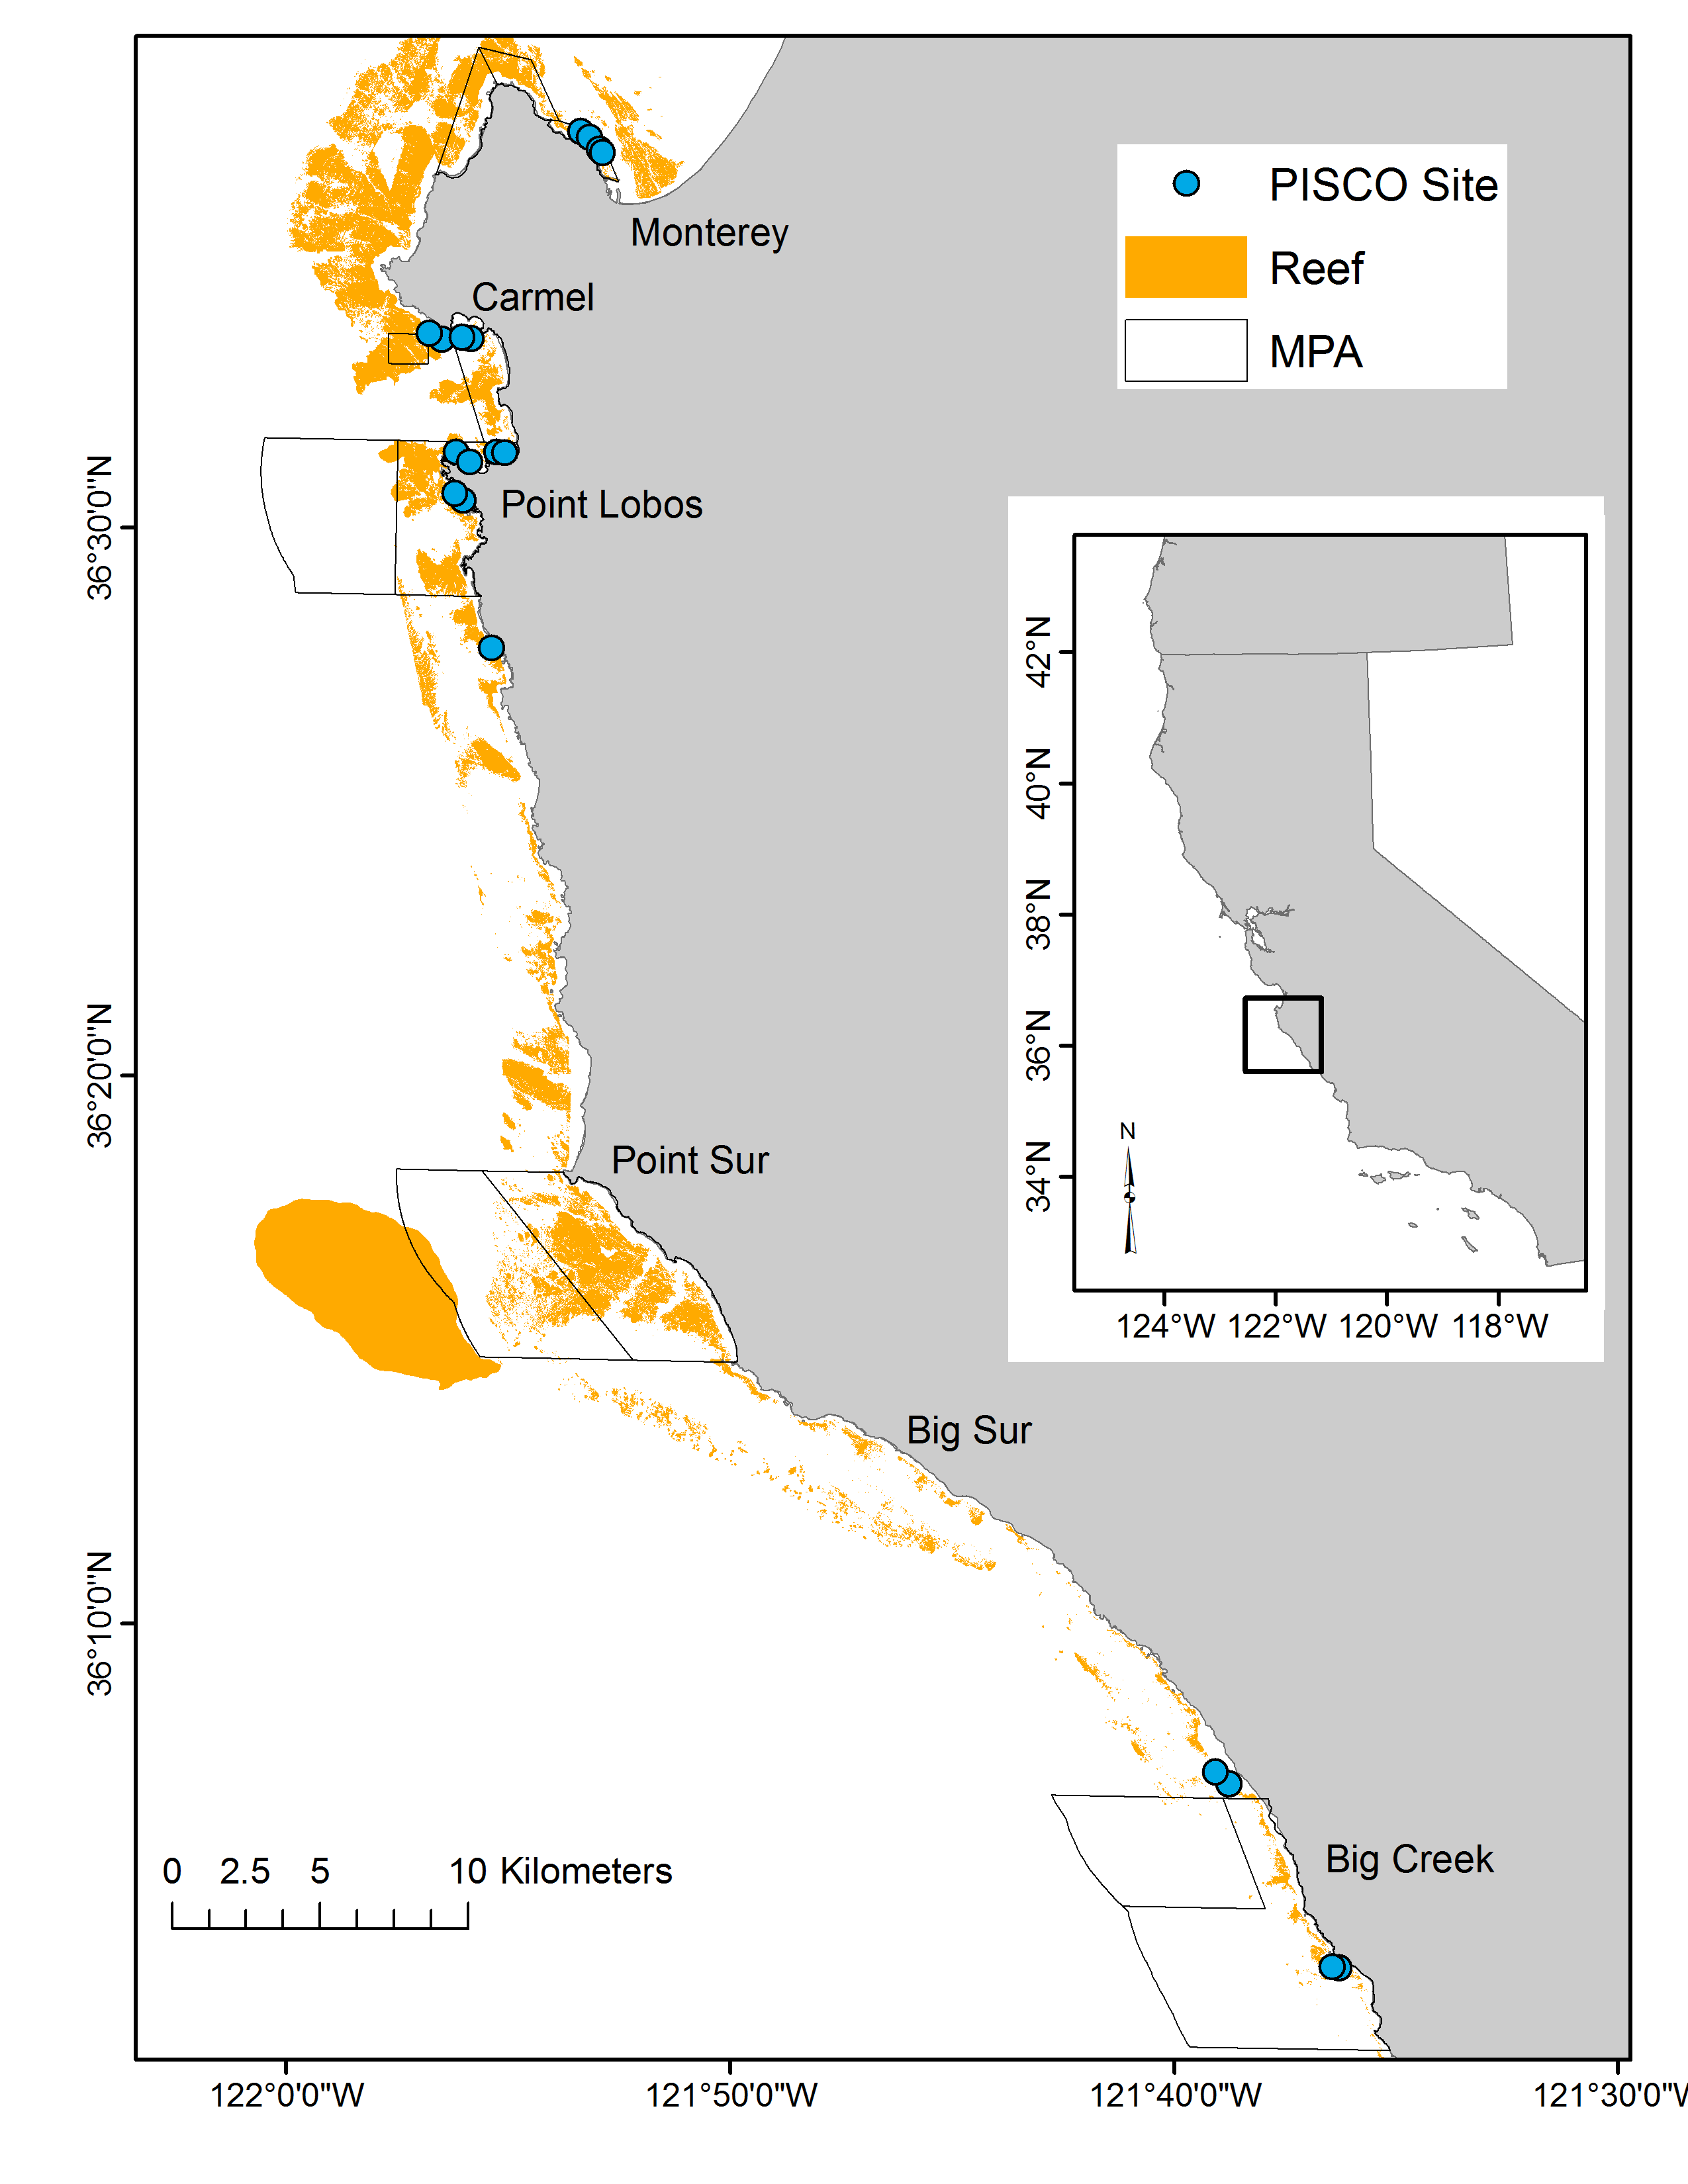
\includegraphics{Figures/PISCO_sites.png}
\caption{Map of the sites sampled consistently through time for the
PISCO kelp forest fish survey. \label{fig:PISCO_sites}}
\end{figure}

\FloatBarrier

\begin{figure}
\centering
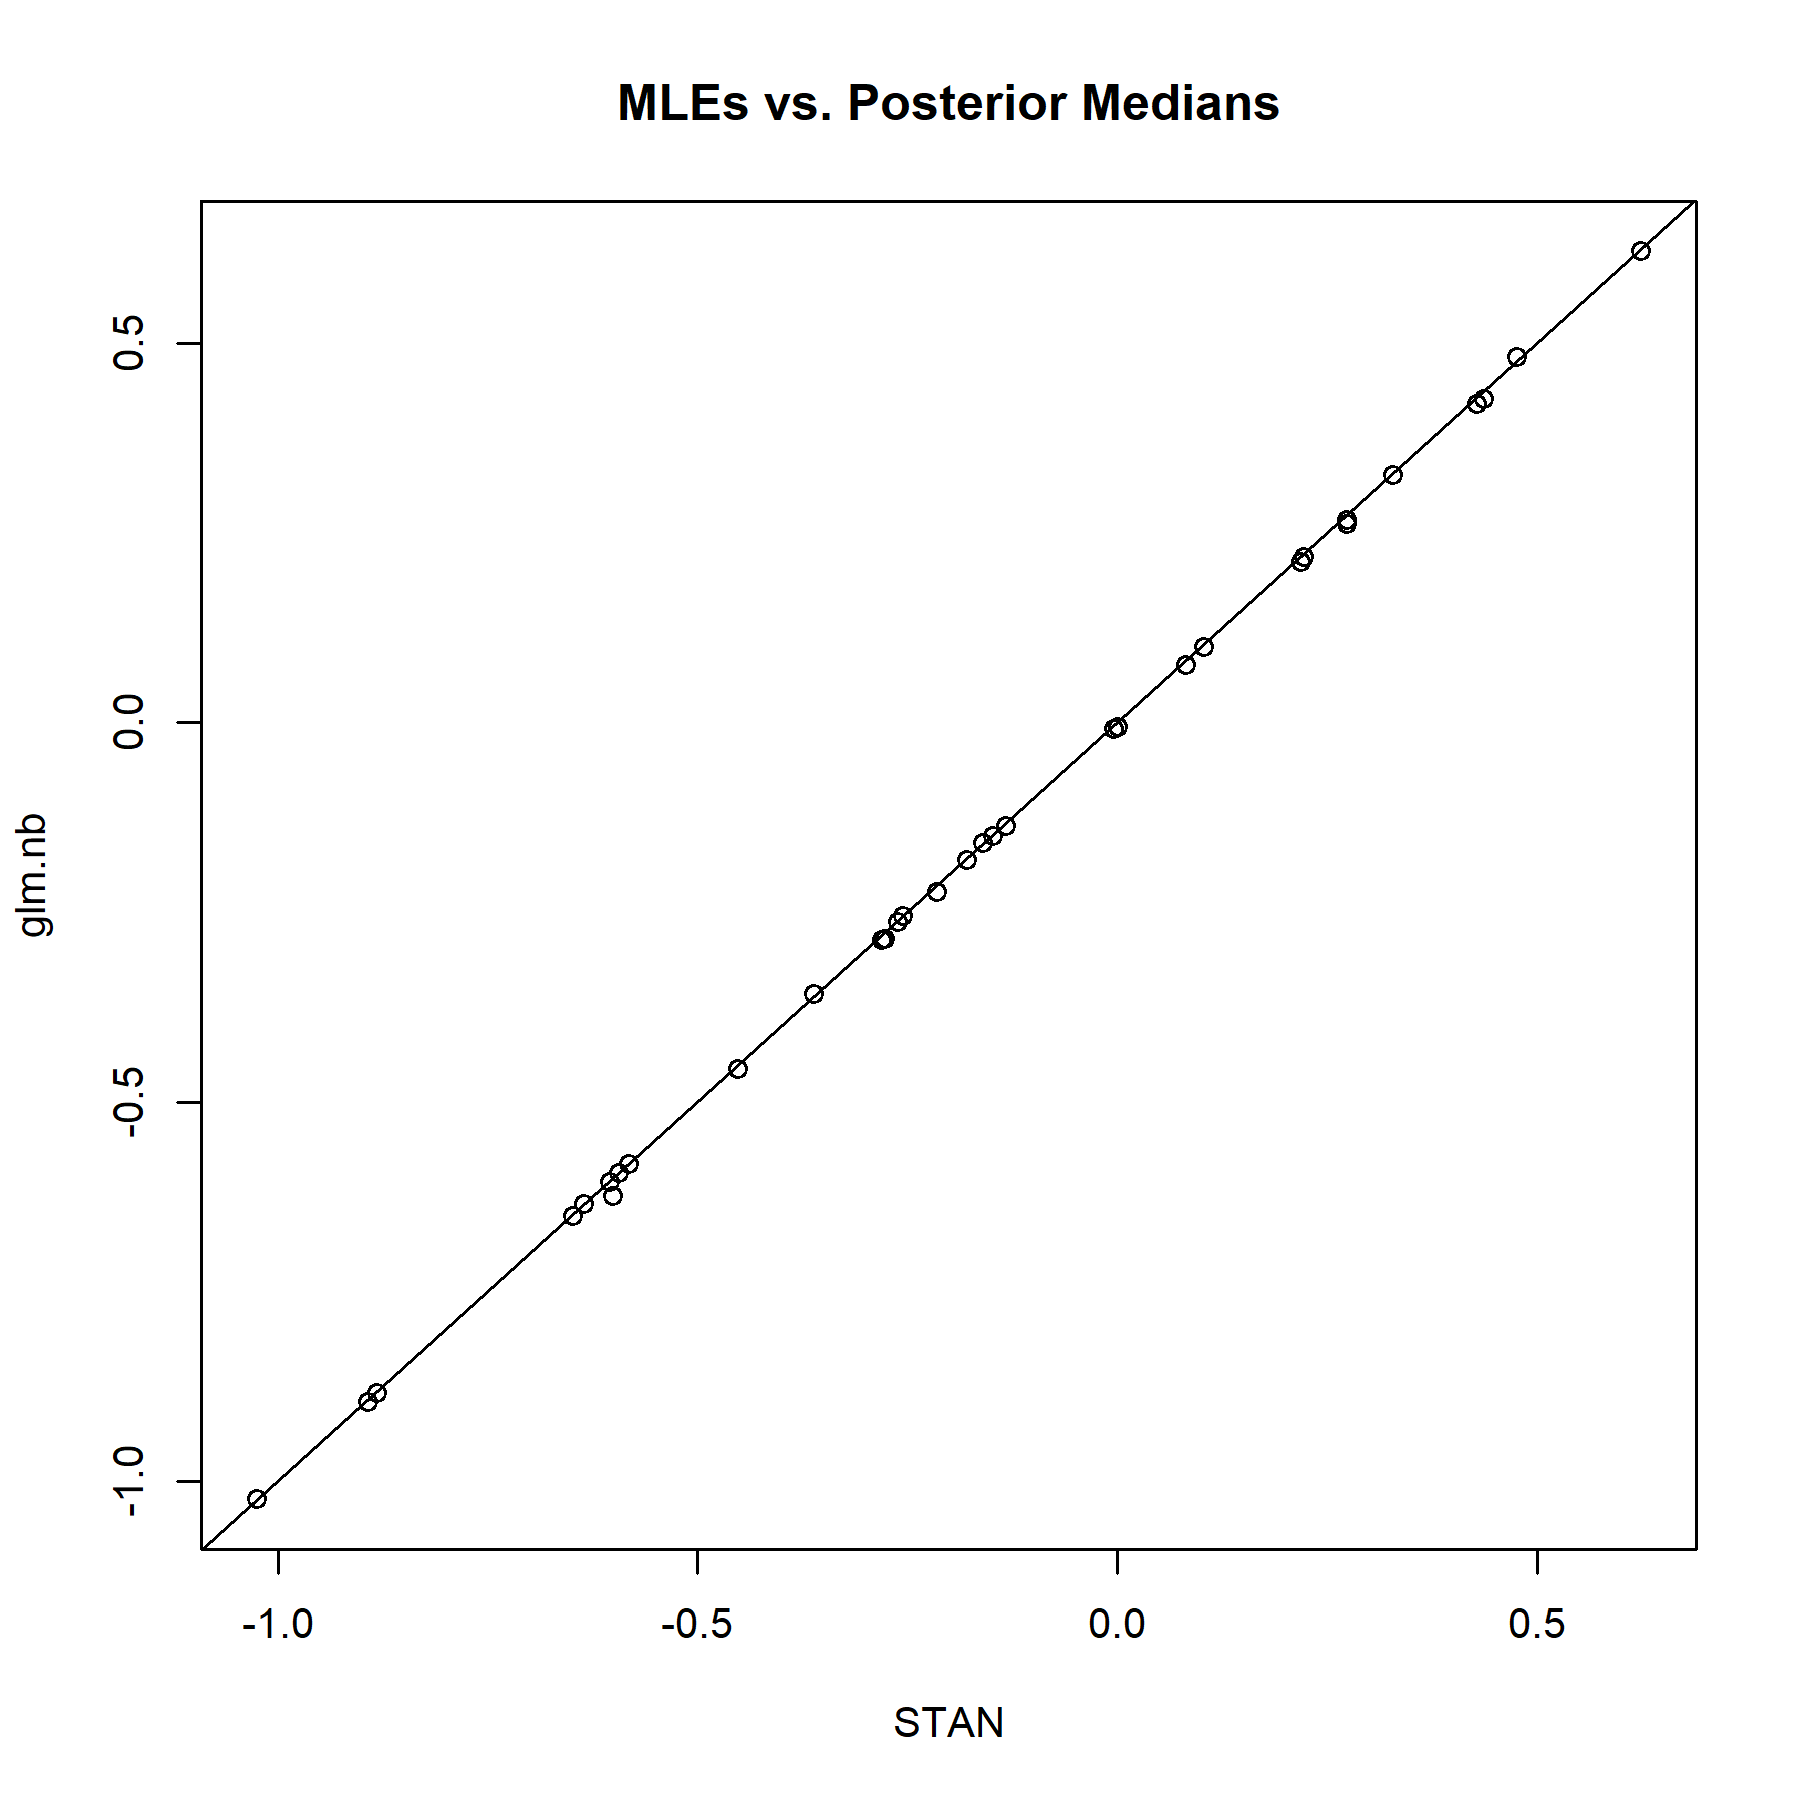
\includegraphics{Figures/Fleet8_MLE_stan.png}
\caption{Comparison of negative bionimial predictions (CPUE) to observed
means in each stratum (year) for the PISCO kelp forest fish survey
index. The 1:1 plot is for reference. \label{fig:Fleet8_MLE_stan}}
\end{figure}

\FloatBarrier

\begin{figure}
\centering
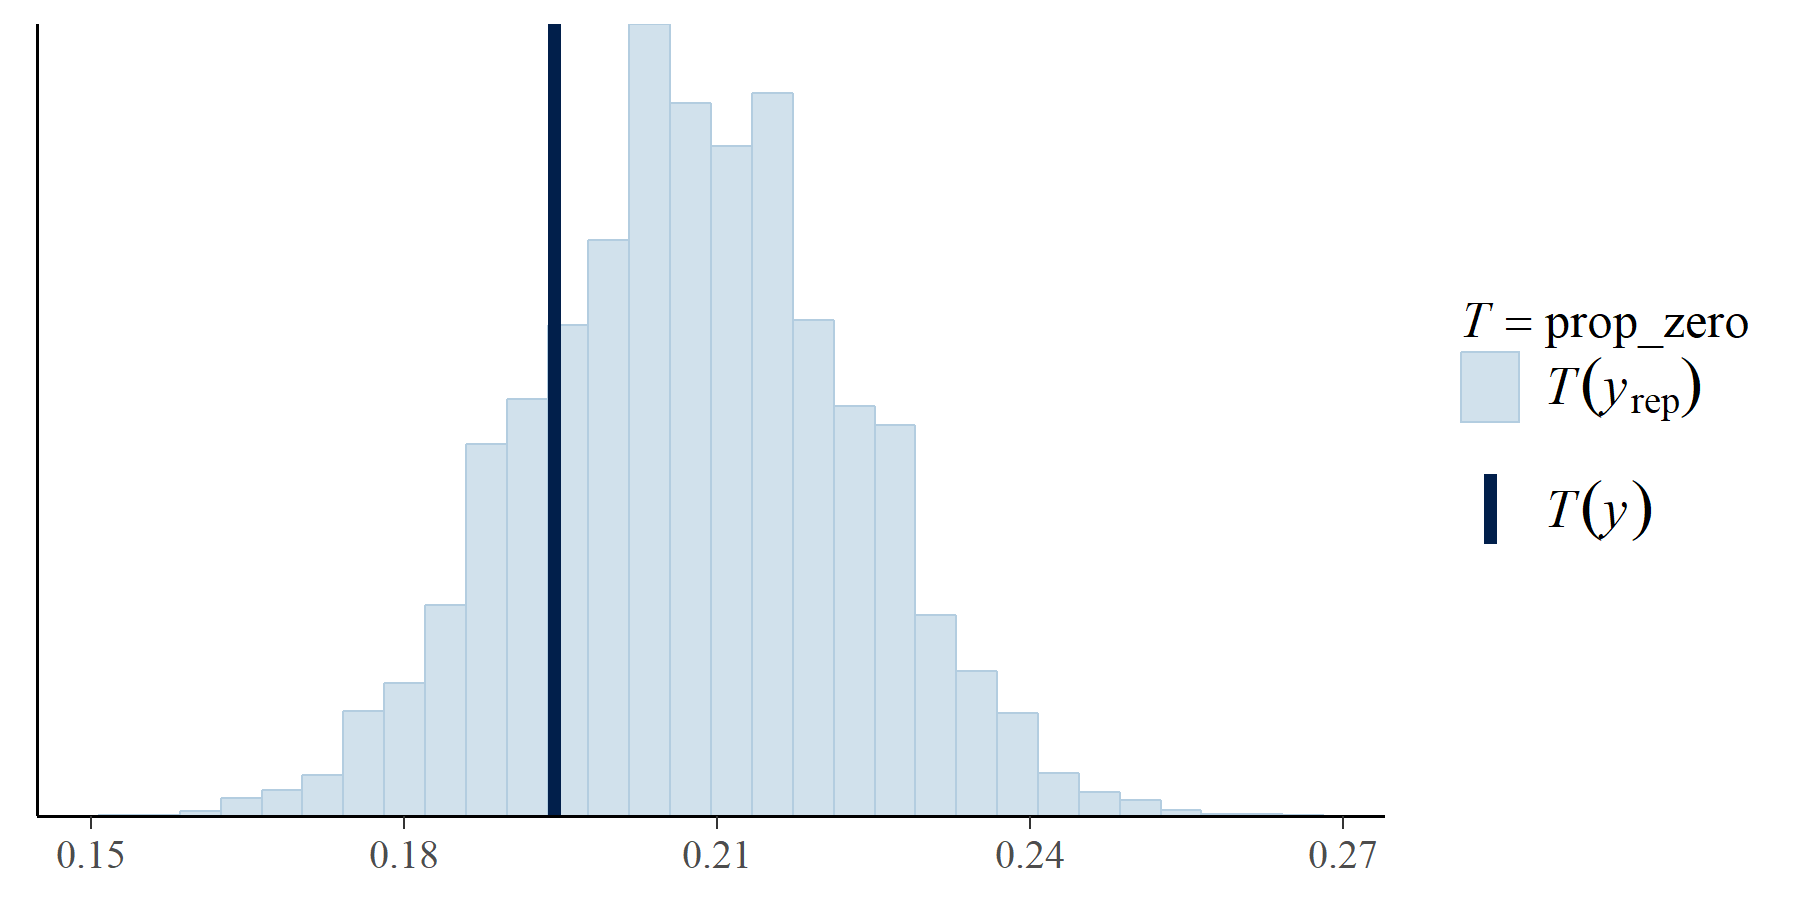
\includegraphics{Figures/Fleet8_prop_zero_STAN.png}
\caption{Posterior predictive distribution of the proportion of zero
observations in replicate data sets generated by the negative binomial
model for the PISCO kelp forest fish survey.
\label{fig:Fleet8_prop_zero_STAN}}
\end{figure}

\FloatBarrier

\begin{figure}
\centering
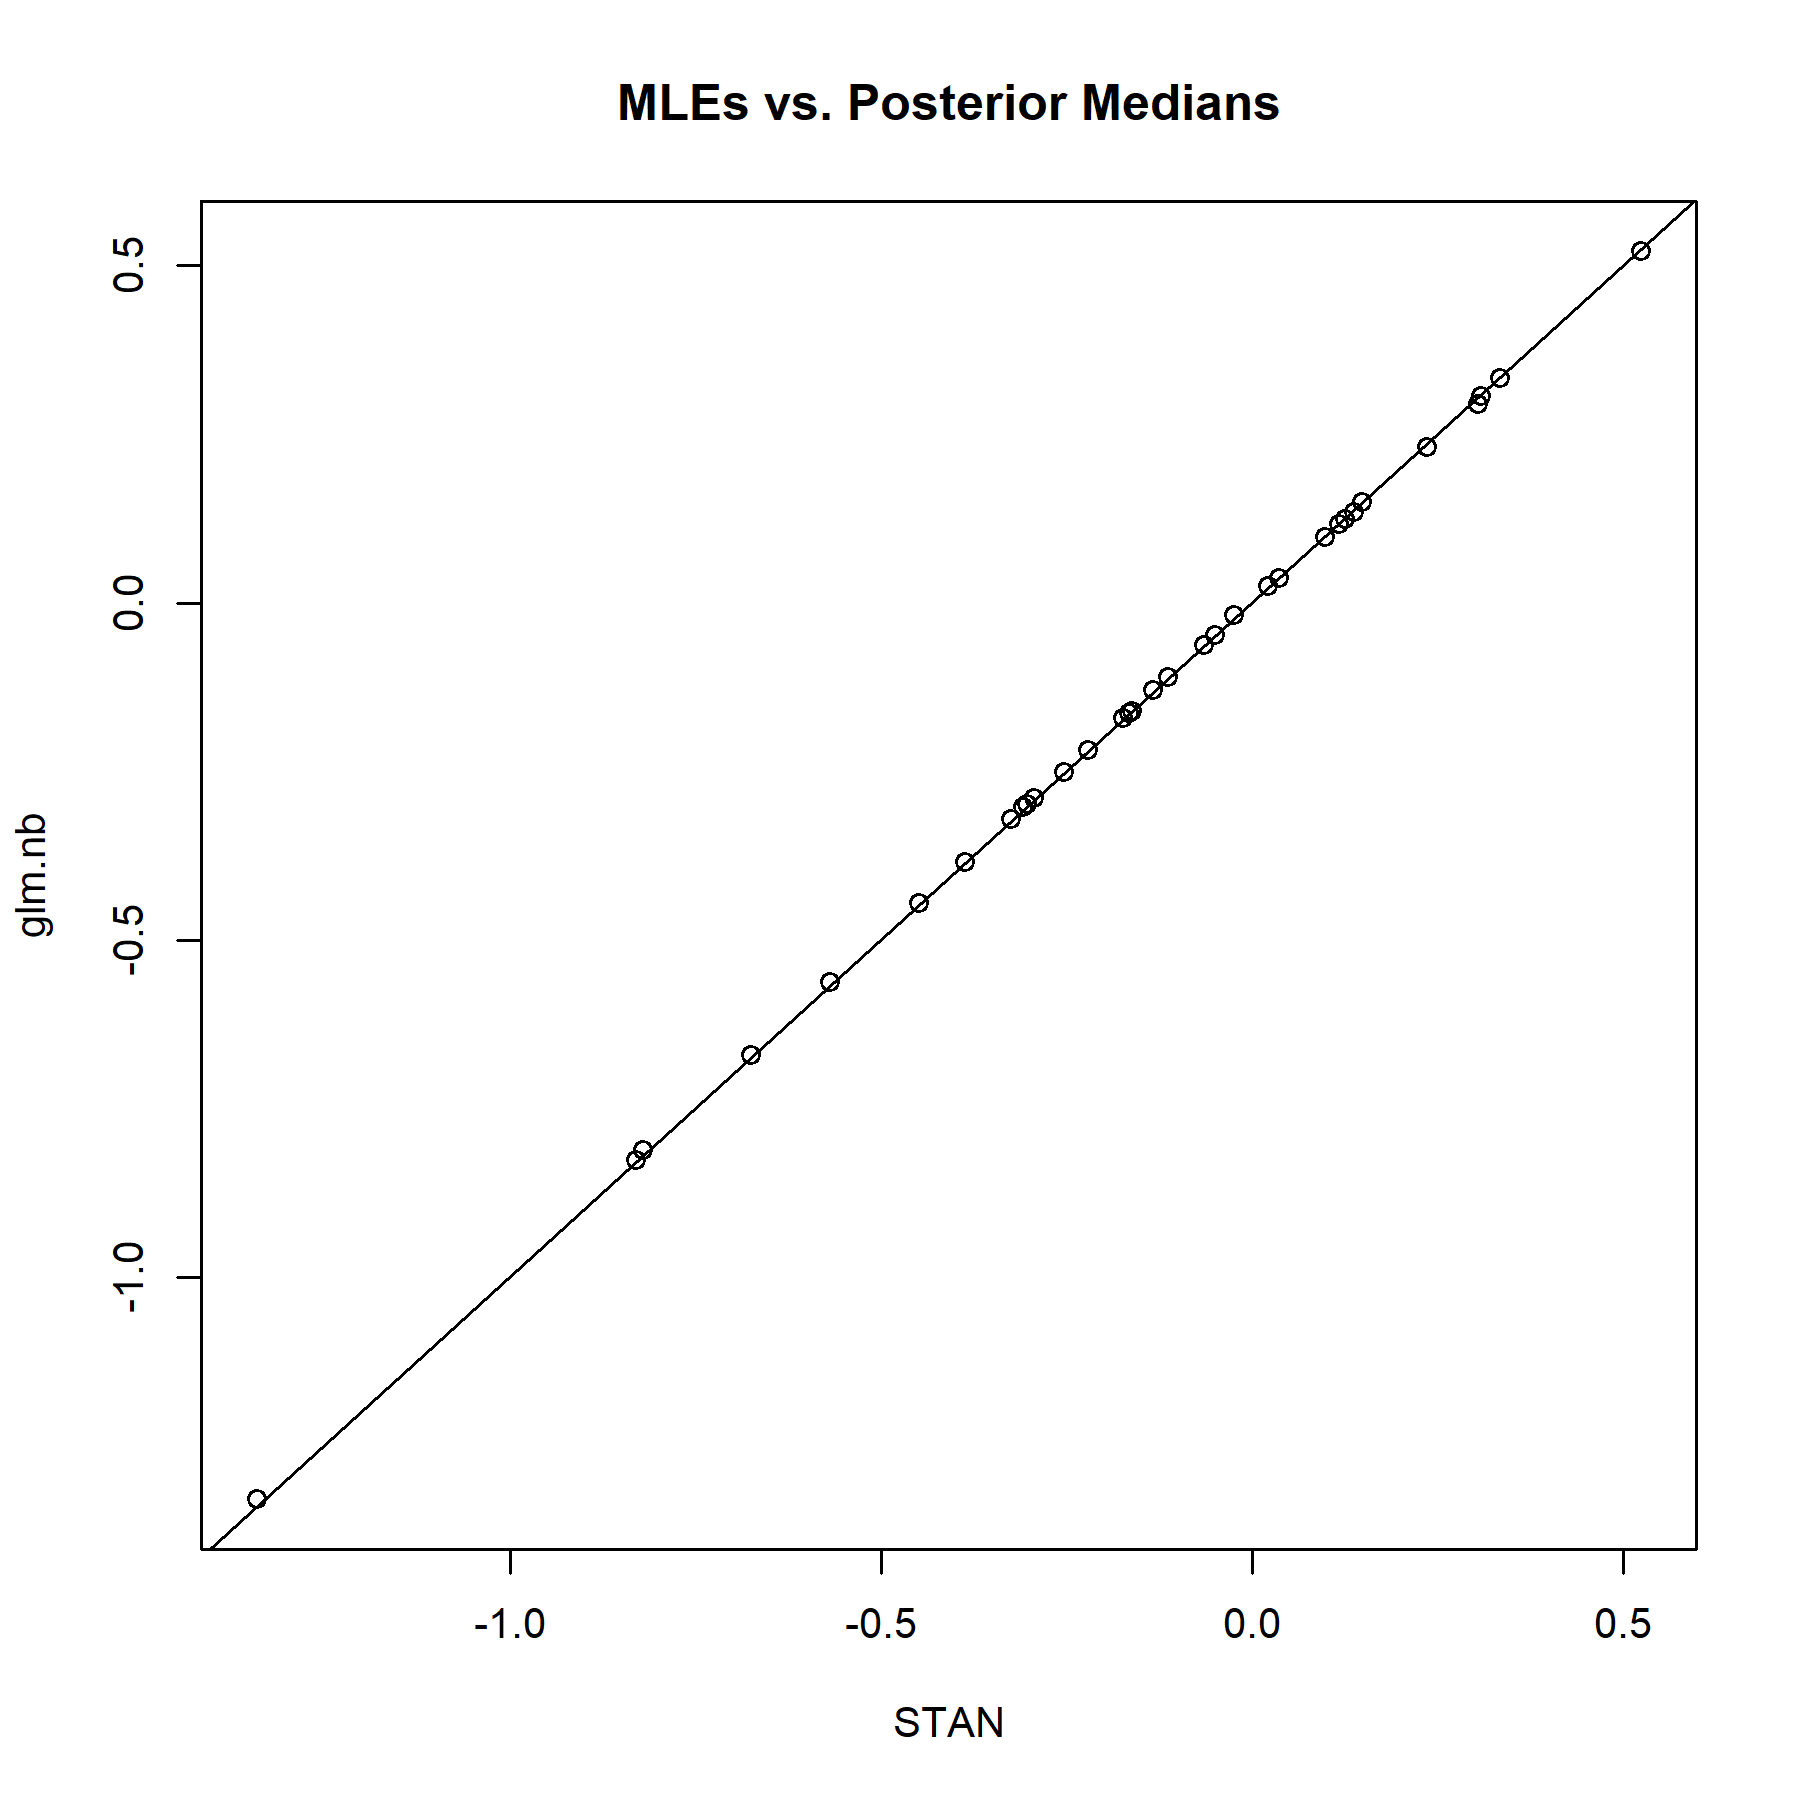
\includegraphics{Figures/Fleet8large_MLE_stan.png}
\caption{Comparison of negative bionimial predictions (CPUE) to observed
means in each stratum (year) for the PISCO kelp forest fish survey index
for fish 15 cm and larger. The 1:1 plot is for reference.
\label{fig:Fleet8large_MLE_stan}}
\end{figure}

\FloatBarrier

\begin{figure}
\centering
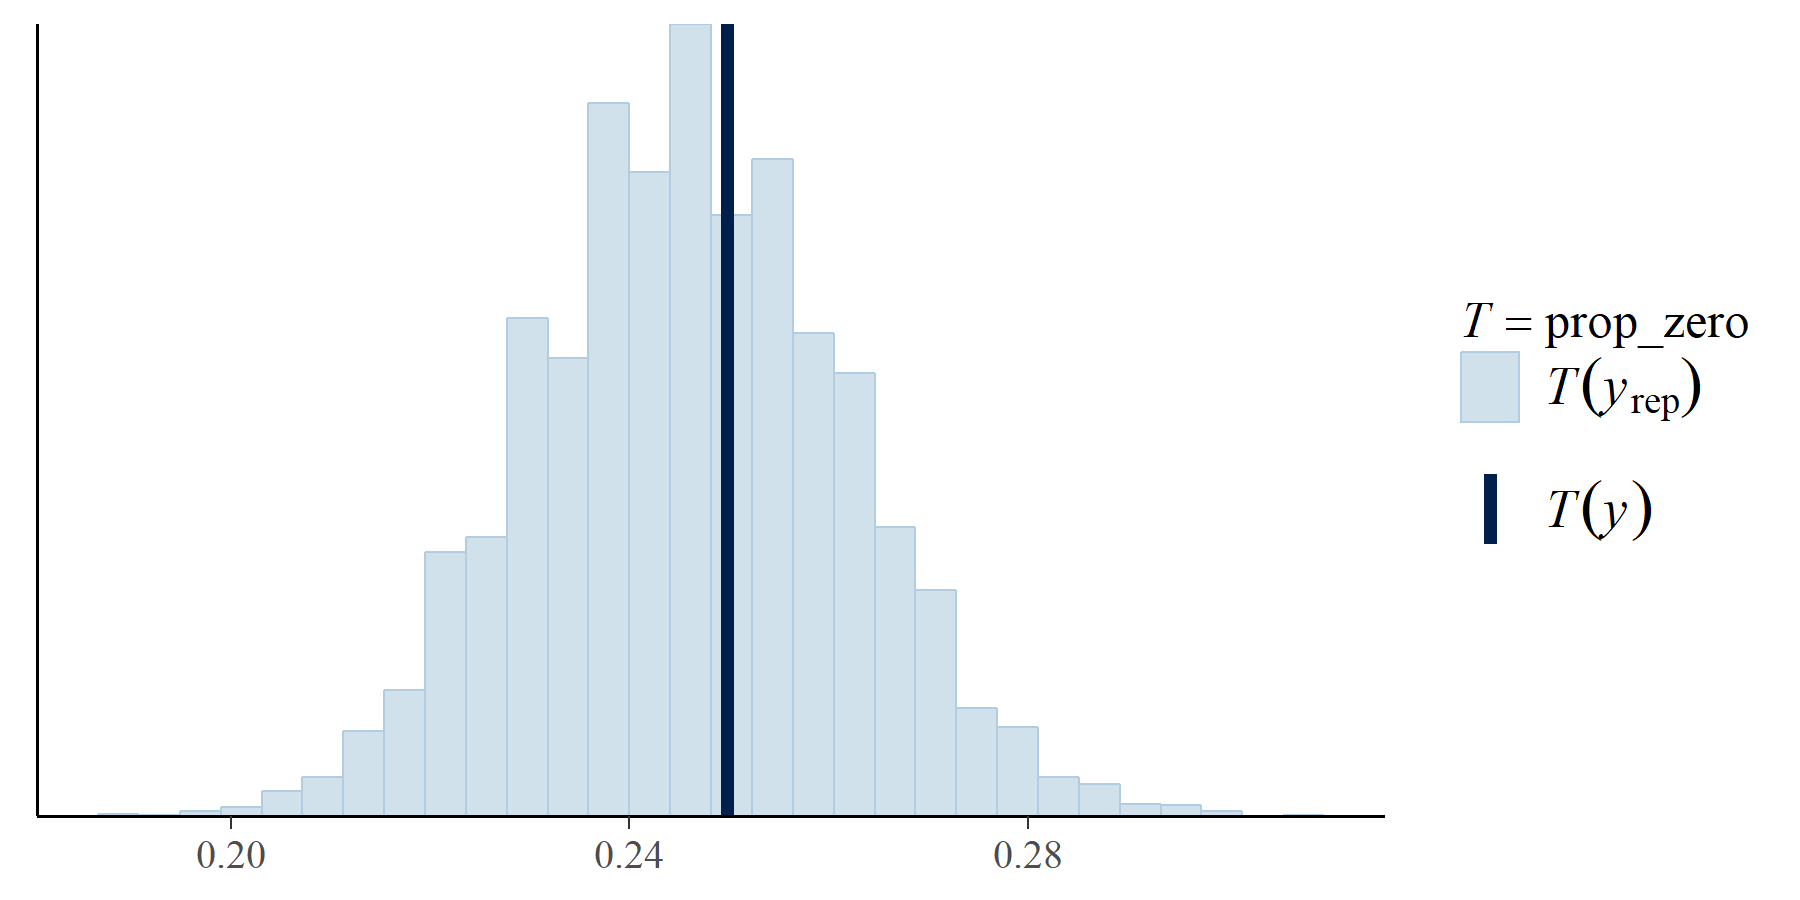
\includegraphics{Figures/Fleet8large_prop_zero_STAN.png}
\caption{Posterior predictive distribution of the proportion of zero
observations in replicate data sets generated by the negative binomial
model for the PISCO kelp forest fish survey for fish 15 cm and larger.
\label{fig:Fleet8large_prop_zero_STAN}}
\end{figure}

\FloatBarrier

\begin{figure}
\centering
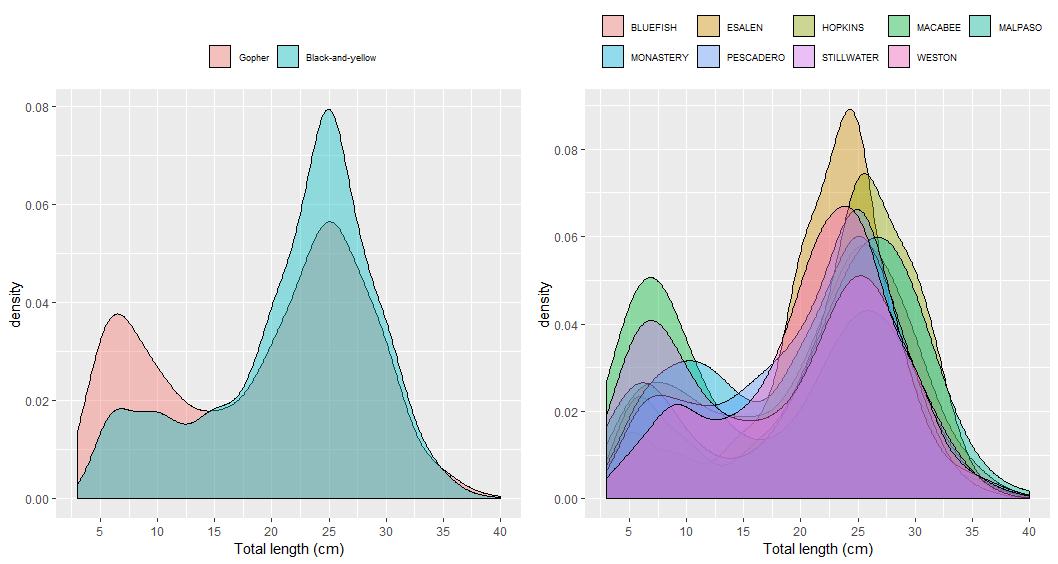
\includegraphics{Figures/PISCO_lengths.png}
\caption{Plots of the length distributions from the PISCO kelp forest
fish survey by species (left) and for combined species by site (right)
for sites included in the final index of abundance.
\label{fig:PISCO_lengths}}
\end{figure}

\FloatBarrier

\begin{figure}
\centering
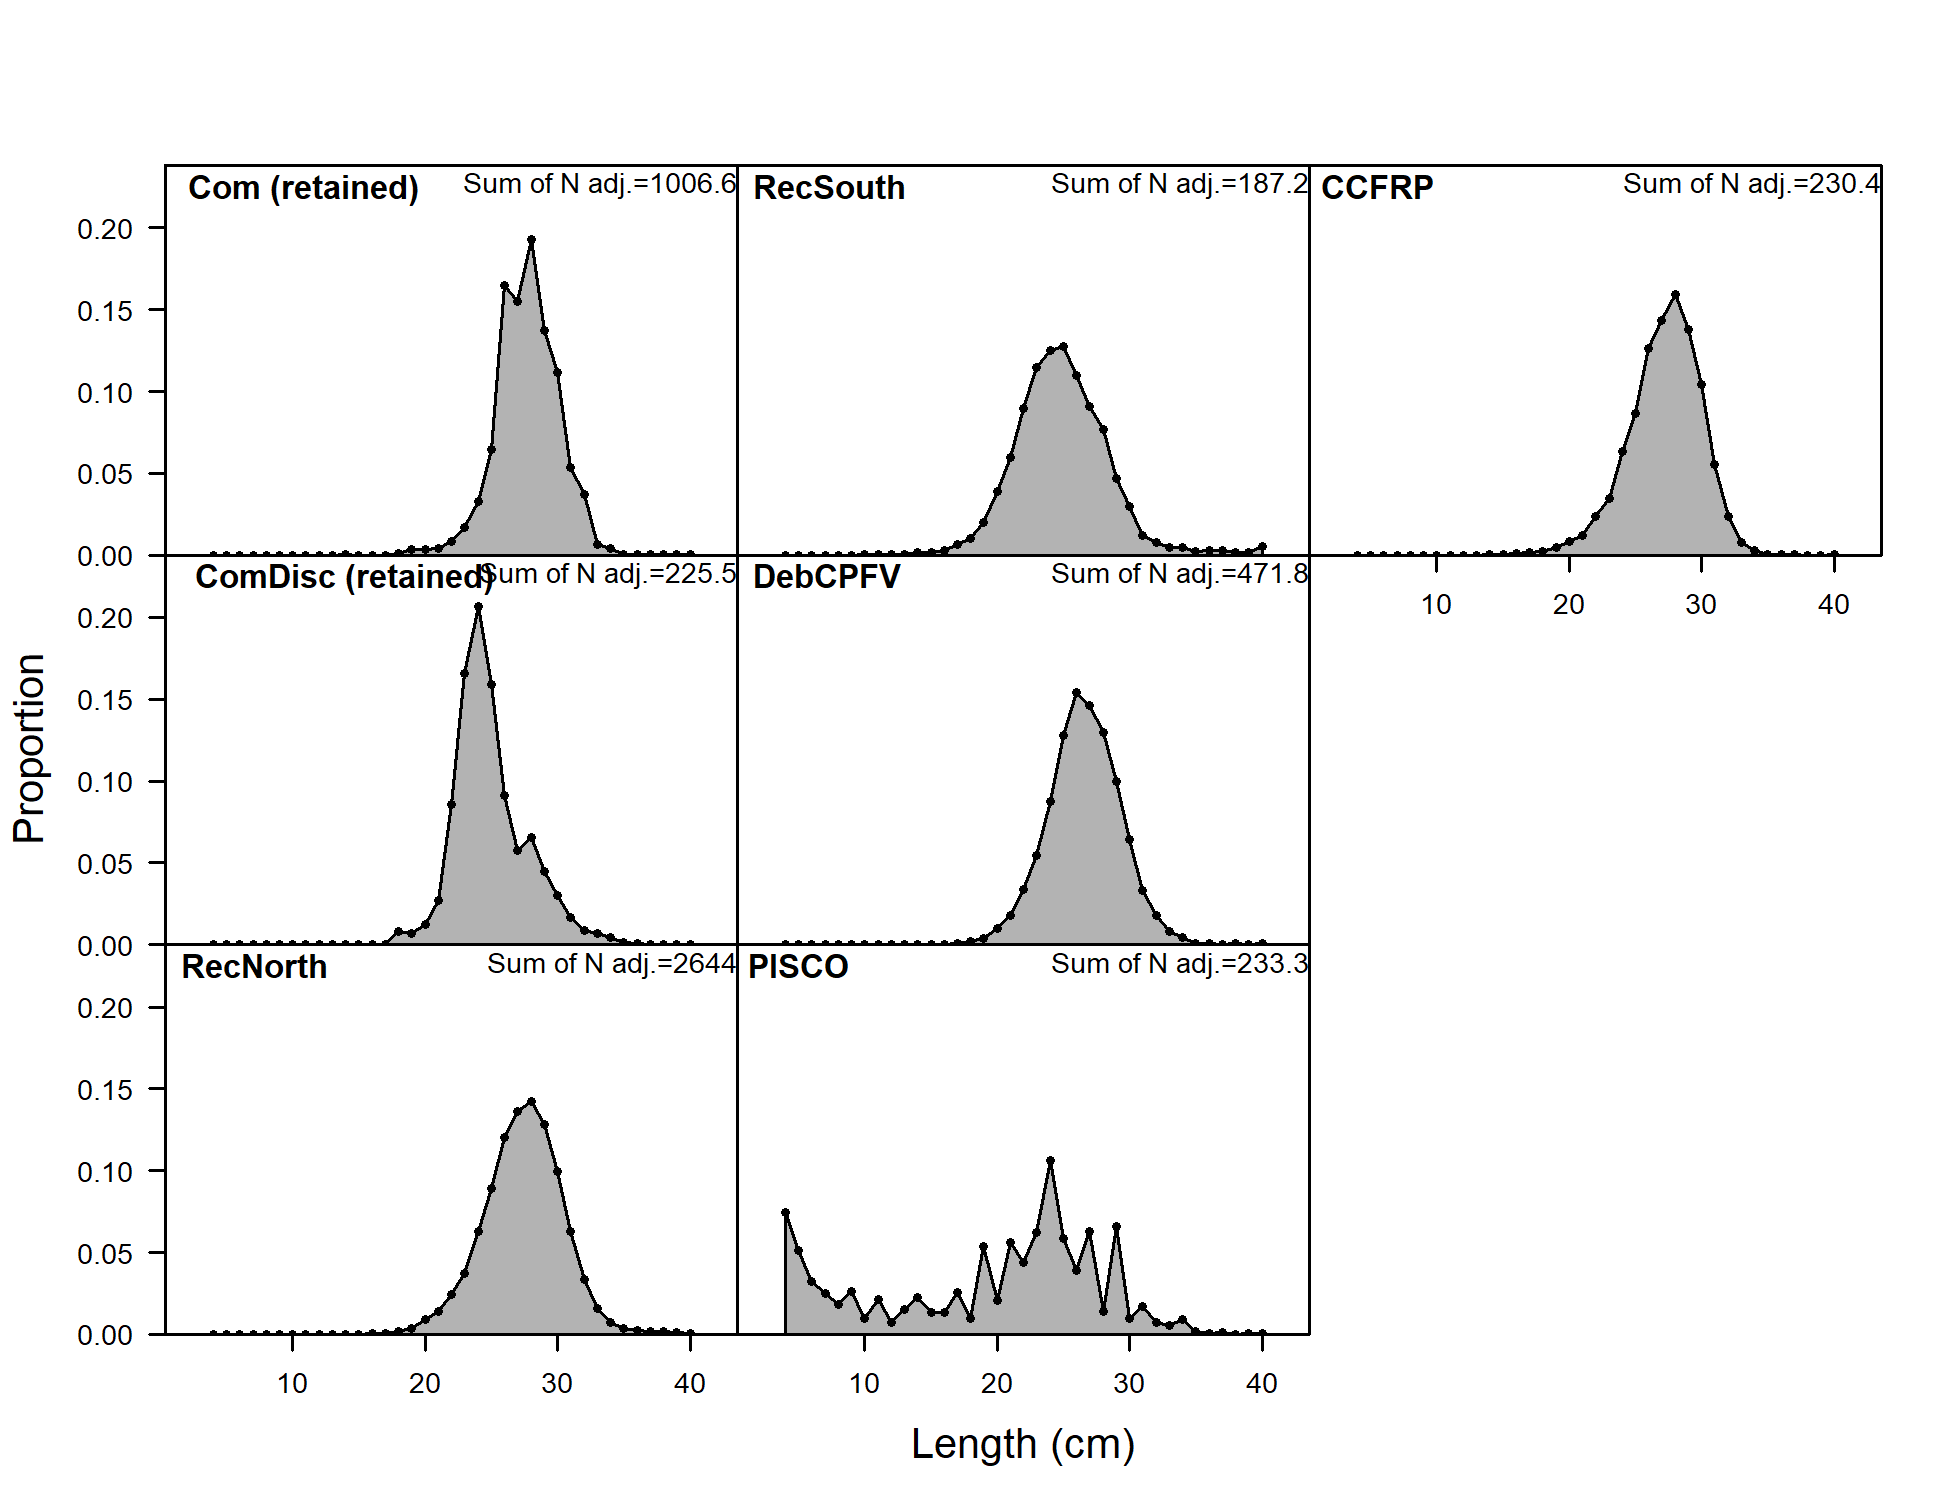
\includegraphics{r4ss/plots_mod1/comp_lendat__aggregated_across_time.png}
\caption{Length comp data, aggregated across time by fleet. Labels
`retained' and `discard' indicate discarded or retained sampled for each
fleet. Panels without this designation represent the whole catch.
\label{fig:comp_lendat_aggregated_across_time}}
\end{figure}

\FloatBarrier

\begin{figure}
\centering
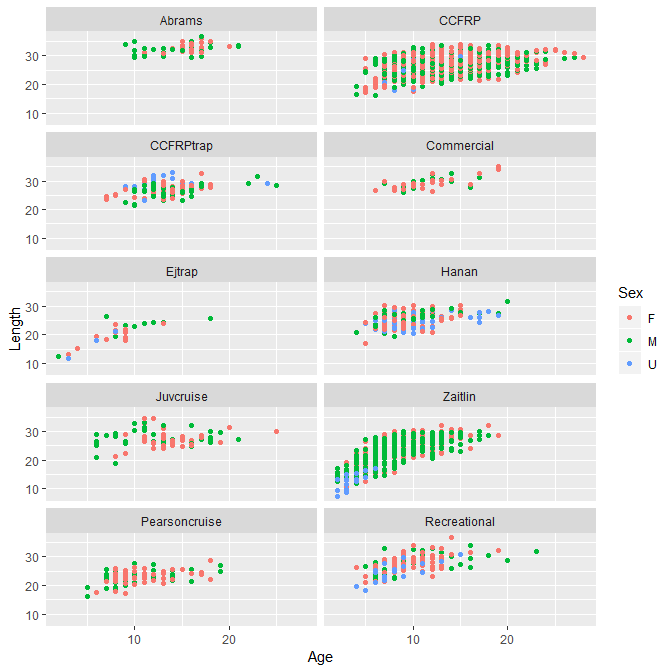
\includegraphics{Figures/Age_length_by_study.png}
\caption{Available length-at-age data for gopher and black-and-yellow
rockfish by sex and data source. The Zaitlin study is all
black-and-yellow rockfish. The remaining plots represent gopher rockfish
\label{fig:Age_length_by_study}}
\end{figure}

\begin{figure}
\centering
\includegraphics{Figures/Growth_by_species.png}
\caption{External estimates of growth for gopher and black-and-yellow
rockfish from fits to von Bertalanffy growth models.
\label{Growth_by_species}}
\end{figure}

\begin{figure}
\centering
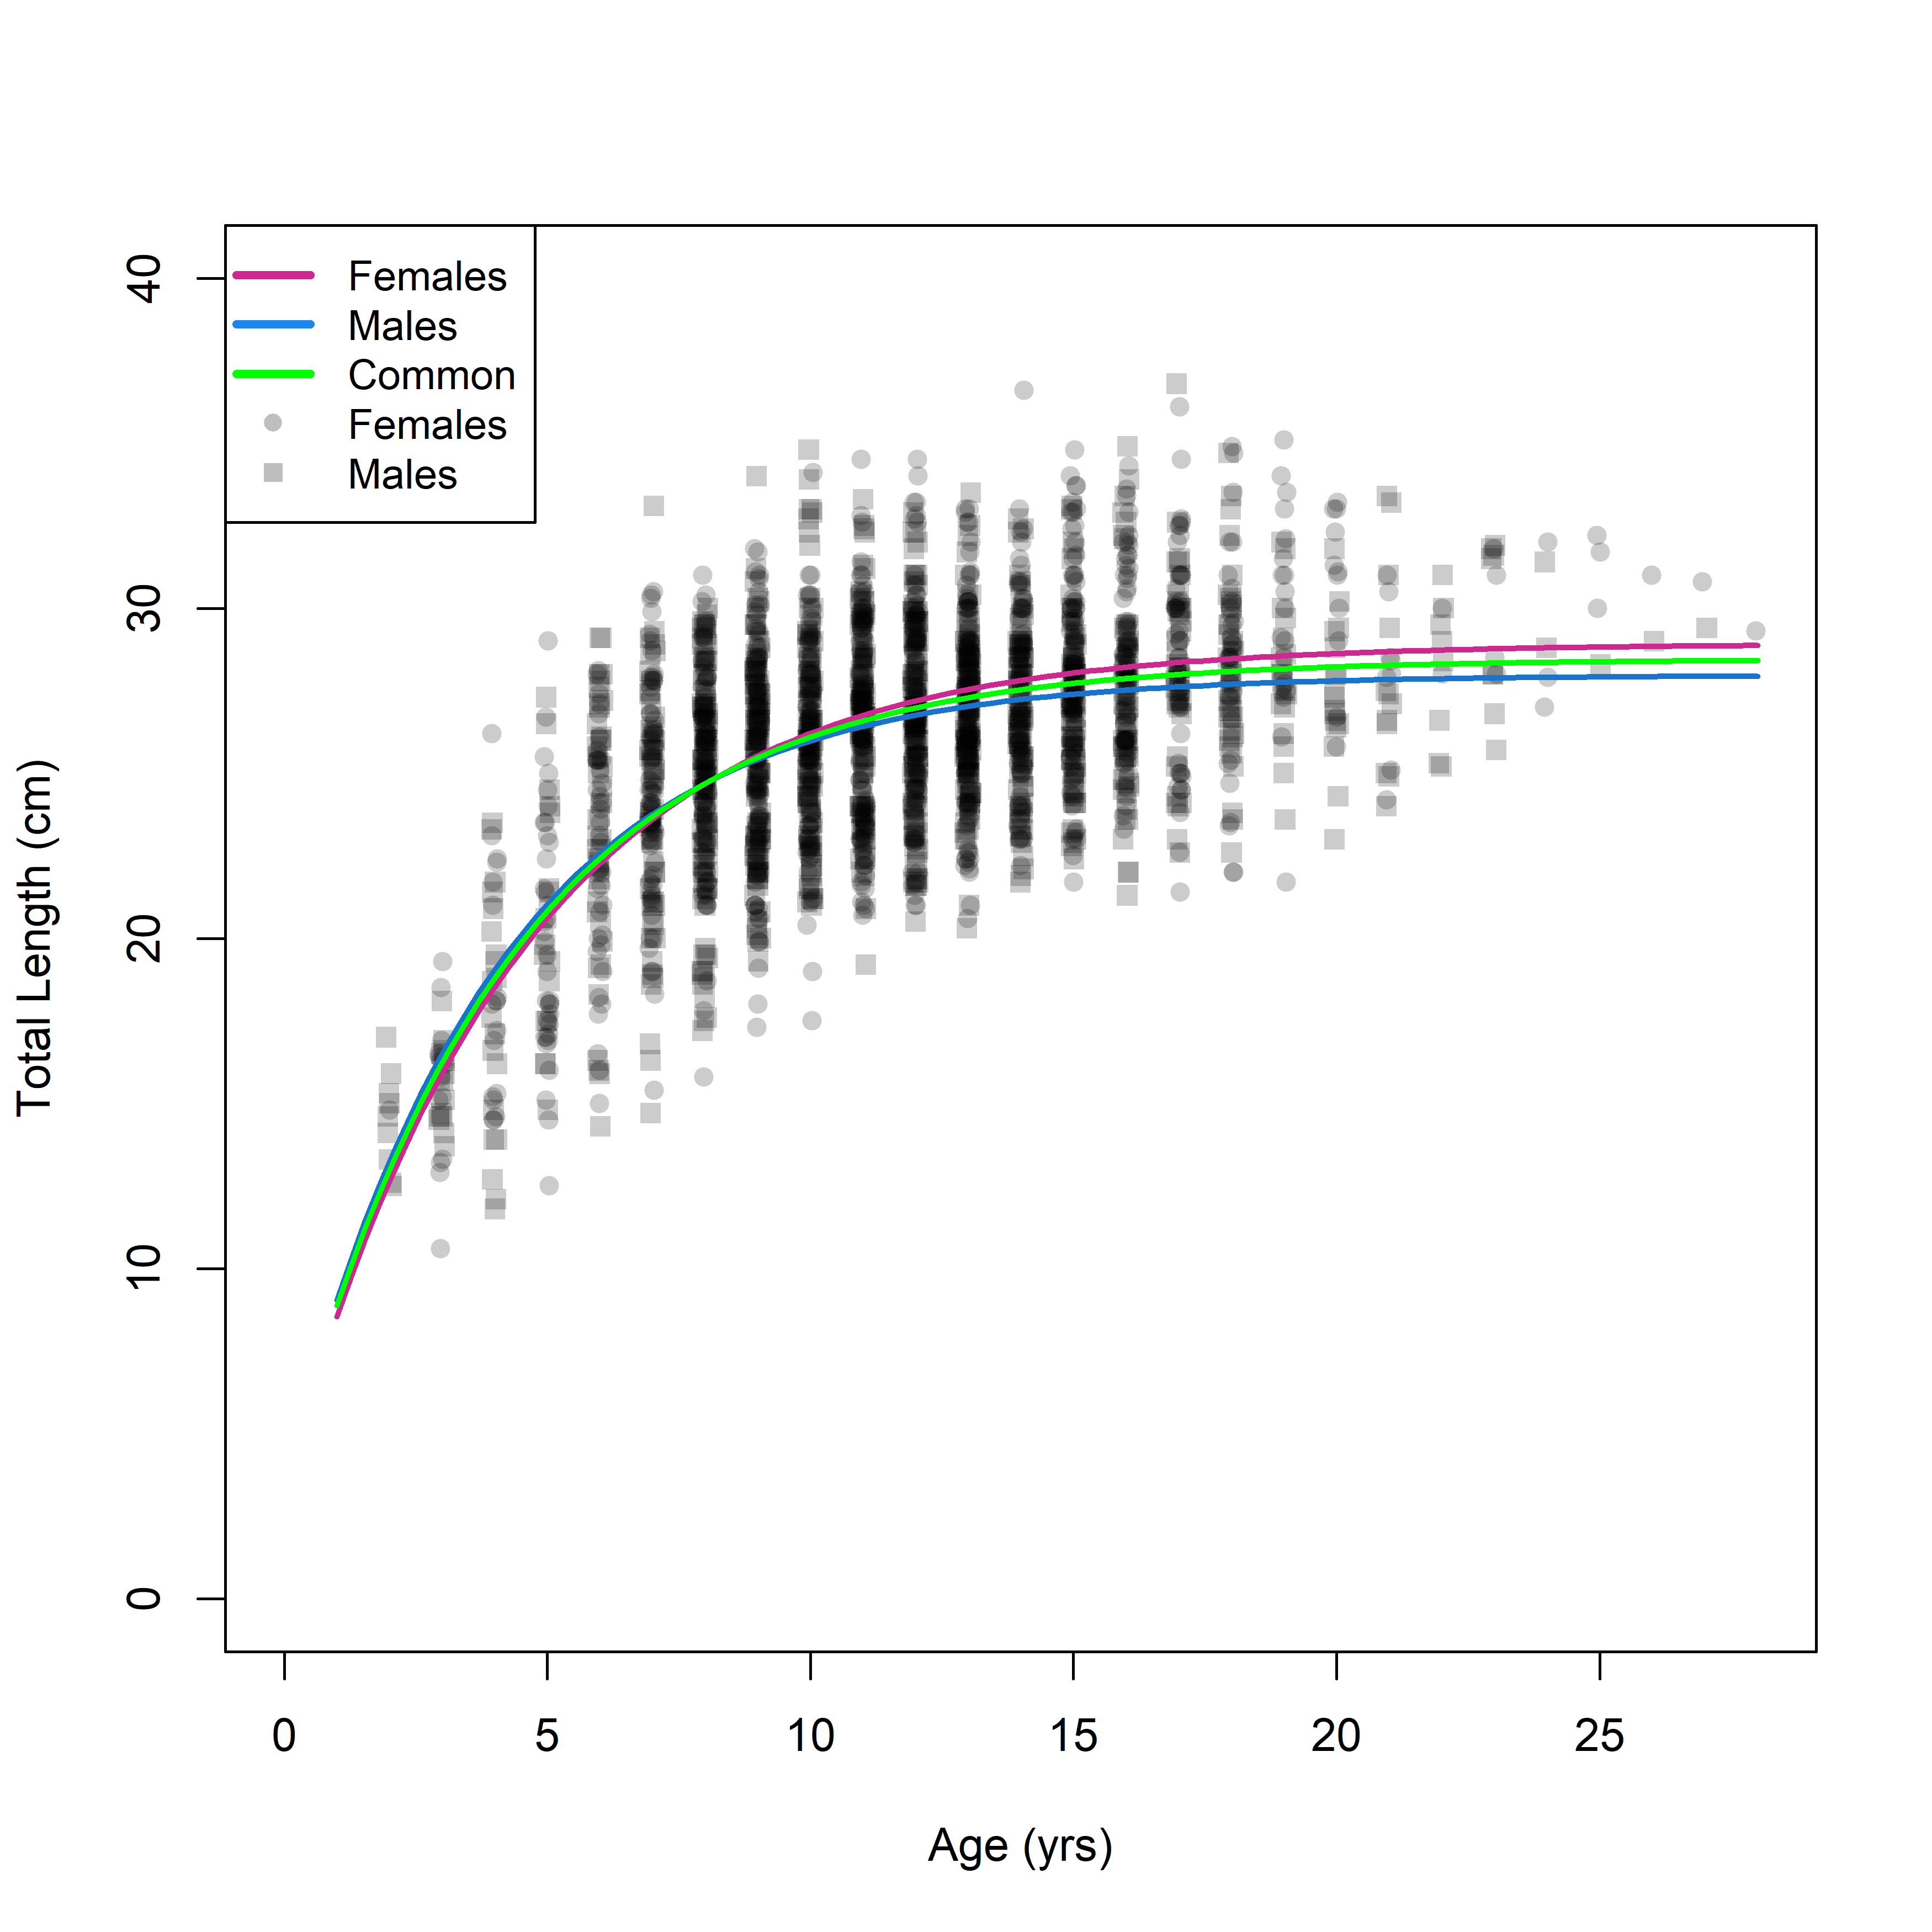
\includegraphics{Figures/Growth_by_sex.png}
\caption{External estimates of growth for GBYR combined by sex from fits
to von Bertalanffy growth models. \label{Growth_by_sex}}
\end{figure}

\FloatBarrier

\begin{figure}
\centering
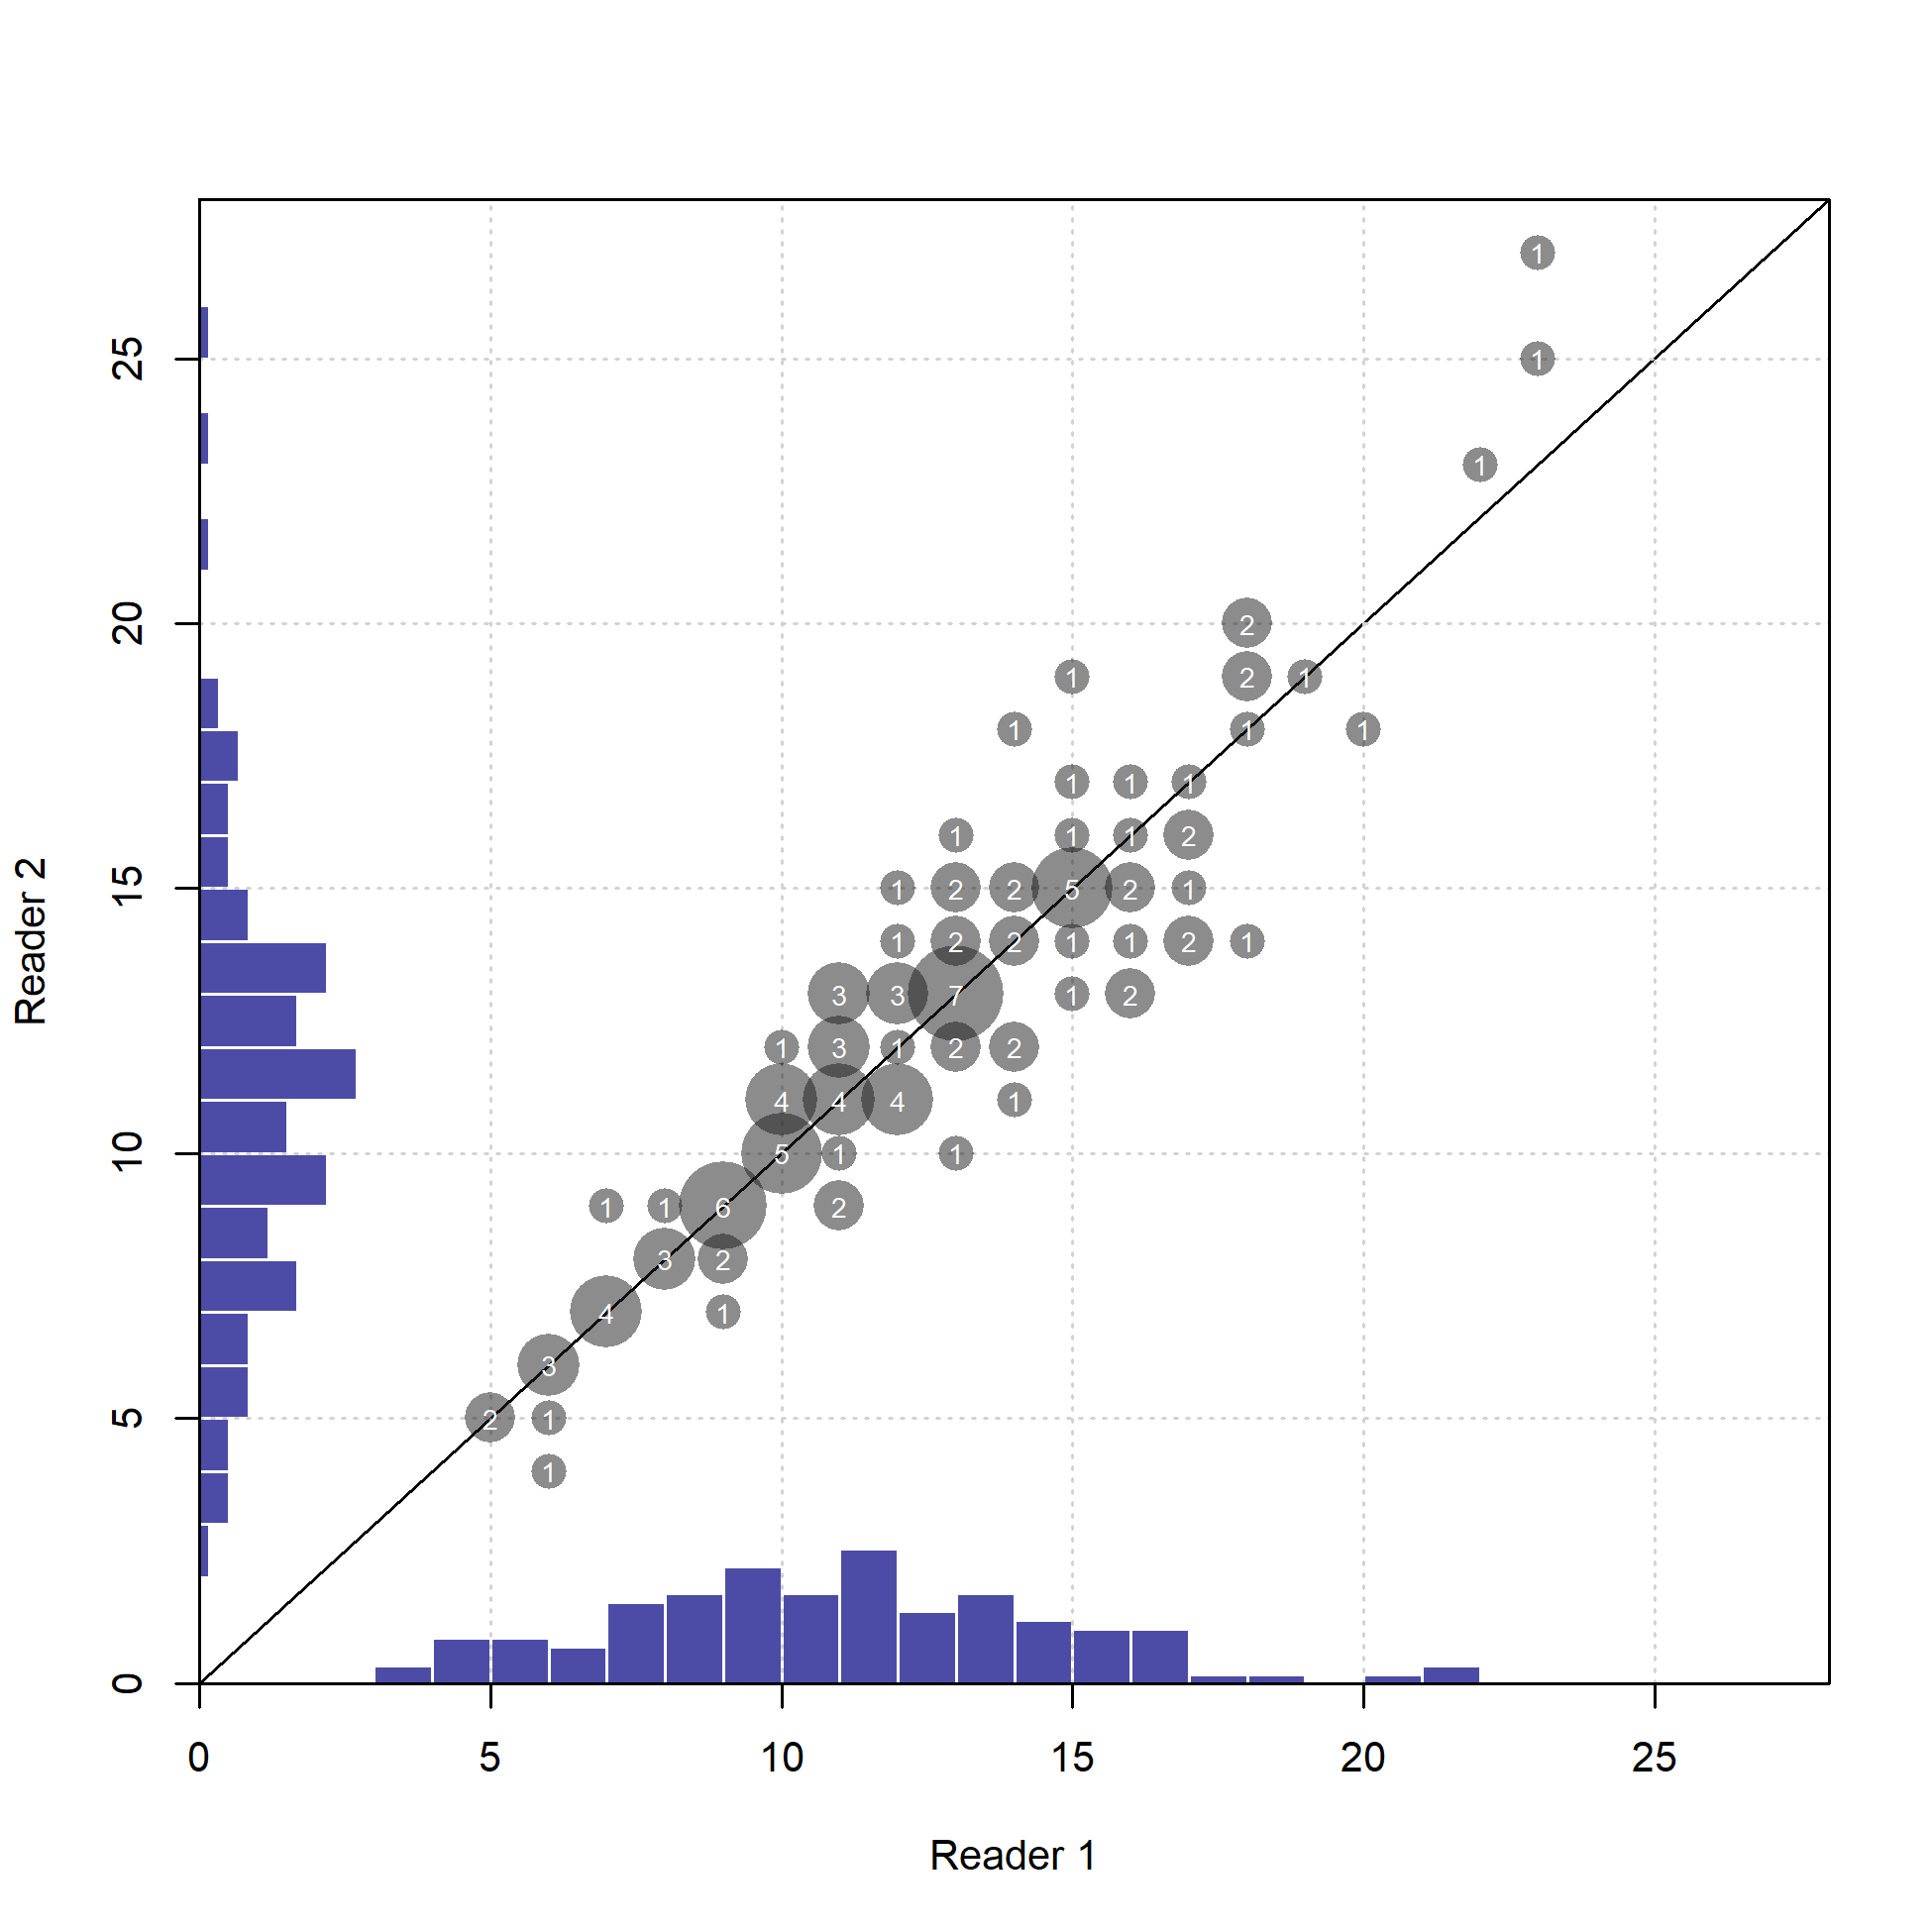
\includegraphics{Figures/GBY_age_error.png}
\caption{Aging precision between initial and blind double reads for
GBYR. Numbers in the bubbles are the sample sizes of otoliths
cross-read. \label{fig:GBY_age_error}}
\end{figure}

\FloatBarrier

\begin{figure}
\centering
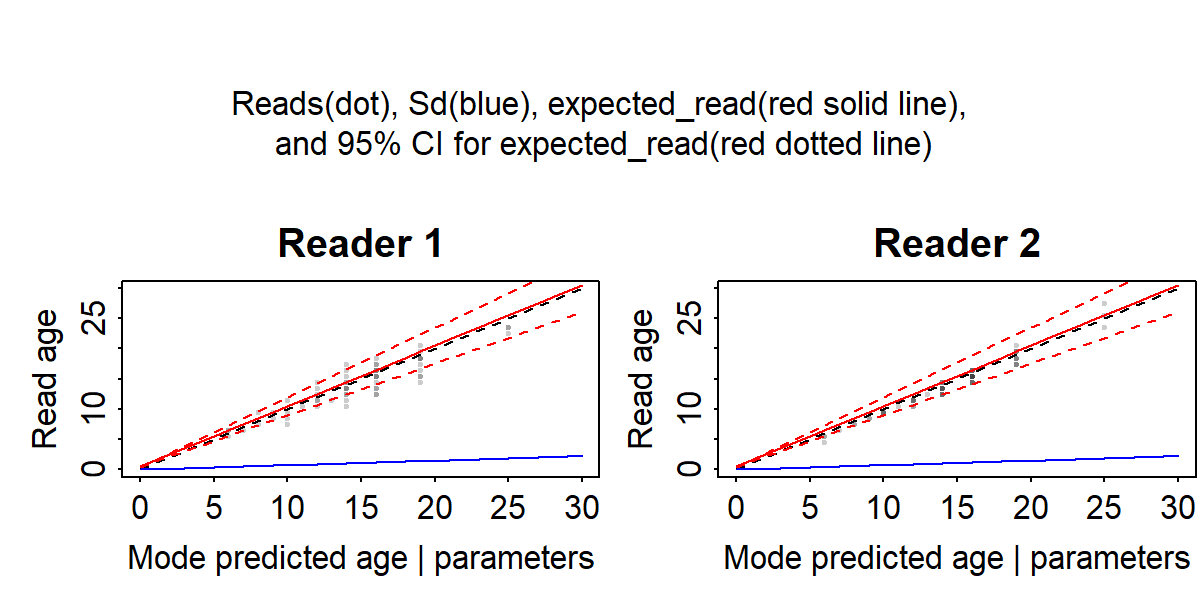
\includegraphics{Figures/GBY_age_error2.png}
\caption{True versus predicted age for two current age readers at the
NWFSC from the ageing error software with unbiased reads and curvilinear
standard deviation for both readers. \label{fig:GBY_age_error2}}
\end{figure}

\begin{figure}
\centering
\includegraphics{Figures/GBY_weight_length.png}
\caption{Comparison of the gopher rockfish weight-length curves from Lea
et al. (1999) and tha estimated from black-and-yellow rockfishes from
Zaitlin (1986), and gopher rockfishes from Loury (2011) and
Meyers-Cherry (2014). The estimated curve from the current data is used
in this assessment. \label{fig:GBY_weight_length}}
\end{figure}

\begin{figure}
\centering
\includegraphics{Figures/GBY_maturity_ogive.png}
\caption{Maturity ogive for females estimated from black-and-yellow
rockfish from Zaitlin (1986) and gopher rockfish from Meyers-Cherry
(2014). Sample sizes at a given length are shown in the circles.
\label{fig:GBY_maturity_ogive}}
\end{figure}

\FloatBarrier

\FloatBarrier

\begin{figure}
\centering
\includegraphics{Figures/SMURF_lengths.png}
\caption{Length distribution by month for GBYR captured using a sampling
tool called a Standard Monitoring Unit for the Recruitment of Fishes
(SMURFs) from the UCSC-PISCO kelp forest fish survey, specifically as
part of Diana Baetscher's dissertation work (Baetscher 2019).
\label{fig:SMURF_lengths}}
\end{figure}

\FloatBarrier

\begin{figure}
\centering
\includegraphics{Figures/Comm_lengths_justification.png}
\caption{Length distributions of gopher and black-and-yellow rockfish
for the commercial fleet and WCGOP discards north and south of Point
Conception. The commercial landings were also separated between fish
landed live and fish landed dead for this figure.
\label{fig:Comm_lengths_justification}}
\end{figure}

\FloatBarrier

\begin{figure}
\centering
\includegraphics{Figures/Rec_lengths_justification.png}
\caption{Length distributions of gopher and black-and-yellow rockfish
for the recreational fleet north and south of Point Conception and by
mode. \label{fig:Rec_lengths_justification}}
\end{figure}

\FloatBarrier

\begin{figure}
\centering
\includegraphics{Figures/sensitivity1_spawnbio.png}
\caption{Sensitivity of the spawning biomass to fixing natural mortality
to the prior, fixing the von Bertalanffy \(k\) parameter to the external
estimate, or using commercial PacFIN length composition data instead of
CALCOM, as compared to the pre-STAR base model.
\label{fig:sensitivity1_spawnbio}}
\end{figure}

\begin{figure}
\centering
\includegraphics{Figures/sensitivity2_spawnbio.png}
\caption{Sensitivity of the spawning biomass to either the default
weight of composition data, the harmonic mean, or Francis weights.
\label{fig:sensitivity2_spawnbio}}
\end{figure}

\FloatBarrier

\begin{figure}
\centering
\includegraphics{Figures/STAR_request1.png}
\caption{Catch curve analysis for age data prior to 2000 and for
2000-2018. \label{fig:STAR_request1}}
\end{figure}

\FloatBarrier

\begin{figure}
\centering
\includegraphics{Figures/STAR_request2.png}
\caption{Comparison of time series of relative and absolute spawning
output from pre-STAR base model and the model from request 2 removing
southern indices. \label{fig:STAR_request2}}
\end{figure}

\begin{figure}
\centering
\includegraphics{Figures/STAR_request3.png}
\caption{Comparison of time series of relative and absolute spawning
output from pre-STAR base model and models from requests 2, 3a and 4.
\label{fig:STAR_request3}}
\end{figure}

\FloatBarrier

\begin{figure}
\centering
\includegraphics{Figures/STAR_request4.png}
\caption{Comparison of time series of recruits from pre-STAR base model
and models from requests 2, 3a and 4a. \label{fig:STAR_request4}}
\end{figure}

\FloatBarrier

\begin{figure}
\centering
\includegraphics{Figures/STAR_request8.png}
\caption{The PISCO recruitment index based upon observed individuals of
4 and 5 cm (``scaled to 5cm'') or 4, 5a and 6 cm (``scaled to 6 cm'').
\label{fig:STAR_request8}}
\end{figure}

\FloatBarrier

\begin{figure}
\centering
\includegraphics{Figures/STAR_request8_2.png}
\caption{Results of request 7 and 8. Time series of absolute (top) and
relative (middle) spawning output and recruitment deviations (now
staring in 1978; bottom). \label{fig:STAR_request8_2}}
\end{figure}

\FloatBarrier

\begin{figure}
\centering
\includegraphics{Figures/STAR_request10.png}
\caption{. Results of request 10, drop-1-out analysis. Time series of
relative (top) and absolute (middle) spawning output and recruitment
estimates (now staring in 1978; bottom). \label{fig:STAR_request10}}
\end{figure}

\begin{figure}
\centering
\includegraphics{Figures/preSTAR_postSTAR_compare_spawnbio}
\caption{Comparison of the spawning output between the pre-STAR panel
base model and the post-STAR model base.
\label{fig:preSTAR_postSTAR_compare_spawnbio}}
\end{figure}

\FloatBarrier

\begin{figure}
\centering
\includegraphics{Figures/preSTAR_postSTAR_compare_Bratio}
\caption{Comparison of the relative spawning output (depletion) between
the pre-STAR panel base model and the post-STAR model base.
\label{fig:preSTAR_postSTAR_compare_Bratio}}
\end{figure}

\begin{figure}
\centering
\includegraphics{Figures/preSTAR_postSTAR_compare_recruit}
\caption{Comparison of the age-0 recruits between the pre-STAR panel
base model and the post-STAR model base.
\label{fig:preSTAR_postSTAR_compare_recruit}}
\end{figure}

\FloatBarrier

\begin{figure}
\centering
\includegraphics{Figures/GBY_age_error_updated.png}
\caption{Updated aging precision used in the post-STAR base model
between initial and blind double reads for GBYR. Numbers in the bubbles
are the sample sizes of otoliths cross-read.
\label{fig:GBY_age_error_updated}}
\end{figure}

\FloatBarrier

\begin{figure}
\centering
\includegraphics{Figures/growth_compare.png}
\caption{Estimates of growth for GBYR from the 2005 assessment, external
fit to the CAAL data used in this assessment and the internal SS
estimate of growth for this assessment. All growth curves were estimated
using the Schnute parameterization of the von Bertalanffy growth curve.
\label{fig:growth_compare}}
\end{figure}

\FloatBarrier

\begin{figure}
\centering
\includegraphics{r4ss/plots_mod1/sel01_multiple_fleets_length1.png}
\caption{Selectivity at length for all of the fleets in the base model.
\label{fig:sel01_multiple_fleets_length1}}
\end{figure}

\FloatBarrier

\begin{figure}
\centering
\includegraphics{r4ss/plots_mod1/recdevs2_withbars.png}
\caption{Estimated time-series of recruitment deviations for GBYR with
95\% intervals. \label{fig:recdevs2_withbars}}
\end{figure}

\begin{figure}
\centering
\includegraphics{r4ss/plots_mod1/ts11_Age-0_recruits_(1000s)_with_95_asymptotic_intervals.png}
\caption{Time series of estimated GBYR recruitments for the base-case
model with 95\% confidence or credibility intervals.
\label{fig:Recruit_mod1}}
\end{figure}

\begin{figure}
\centering
\includegraphics{r4ss/plots_mod1/recruit_fit_bias_adjust.png}
\caption{Bias adjustment for recruitment deviations. Points are
transformed variances. Red line shows current settings for bias
adjustment specified in the control file. Blue line shows the least
squares estimate of alternative bias adjustment relationship for
recruitment deviations. \label{fig:recruit_fit_bias_adjust}}
\end{figure}

\begin{figure}
\centering
\includegraphics{r4ss/plots_mod1/SR_curve2.png}
\caption{Estimated recruitment (red circles) and the assumed
stock-recruit relationship (black line) for GBYR. The green line shows
the effect of the bias correction for the lognormal distribution.
\label{fig:SR_curve2}}
\end{figure}

\FloatBarrier 

\begin{figure}
\centering
\includegraphics{r4ss/plots_mod1/index5_logcpuefit_RecDocksideNorth.png}
\caption{Fit to log index data on log scale for the recreational MRFSS
dockside CPFV fishery north of Point Conception. Lines indicate 95\%
uncertainty interval around index values. Thicker lines indicate input
uncertainty before addition of estimated additional uncertainty
parameter. \label{fig:index5_logcpuefit_RecDocksideNorth}}
\end{figure}

\FloatBarrier

\begin{figure}
\centering
\includegraphics{r4ss/plots_mod1/index5_logcpuefit_DebCPFV.png}
\caption{Fit to log index data on log scale for the recreational Deb's
CPFV onboard observer program, representing north of Point Conception.
Lines indicate 95\% uncertainty interval around index values. Thicker
lines indicate input uncertainty before addition of estimated additional
uncertainty parameter. \label{fig:index5_logcpuefit_DebCPFV}}
\end{figure}

\FloatBarrier 

\begin{figure}
\centering
\includegraphics{r4ss/plots_mod1/index5_logcpuefit_RecOnboardNorth.png}
\caption{Fit to log index data on log scale for the CRFS/Cal Poly CPFV
onboard observer survey north of Point Conception. Lines indicate 95\%
uncertainty interval around index values. Thicker lines indicate input
uncertainty before addition of estimated additional uncertainty
parameter. \label{fig:index5_logcpuefit_RecOnboardNorth}}
\end{figure}

\FloatBarrier

\begin{figure}
\centering
\includegraphics{r4ss/plots_mod1/index5_logcpuefit_PISCO.png}
\caption{Fit to log index data on log scale for the fishery-independent
PISCO kelp forest fish survey for fish 15 cm and larger. Lines indicate
95\% uncertainty interval around index values. Thicker lines indicate
input uncertainty before addition of estimated additional uncertainty
parameter. \label{fig:index5_logcpuefit_PISCO}}
\end{figure}

\FloatBarrier 

\begin{figure}
\centering
\includegraphics{r4ss/plots_mod1/index5_logcpuefit_PISCOage0.png}
\caption{Fit to log index data on log scale for the fishery-independent
PISCO age-0 (6 cm or less) kelp forest fish survey for fish 15 cm and
larger. Lines indicate 95\% uncertainty interval around index values.
\label{fig:index5_logcpuefit_PISCOage0}}
\end{figure}

\FloatBarrier

\begin{figure}
\centering
\includegraphics{r4ss/plots_mod1/index5_logcpuefit_CCFRP.png}
\caption{Fit to log index data on log scale for the fishery-independent
CCFRP hook-and-line survey. Lines indicate 95\% uncertainty interval
around index values. Thicker lines indicate input uncertainty before
addition of estimated additional uncertainty parameter.
\label{fig:index5_logcpuefit_CCFRP}}
\end{figure}

\FloatBarrier 

\begin{figure}
\centering
\includegraphics{r4ss/plots_mod1/comp_lenfit__aggregated_across_time.png}
\caption{Length compositions aggregated across time by fleet.
\label{fig:comp_lenfit__aggregated_across_time}}
\end{figure}

\FloatBarrier

\begin{figure}
\centering
\includegraphics{r4ss/plots_mod1/comp_condAALfit_data_weighting_TA1.8_condAgeRecNorth.png}
\caption{Mean age for the recreational fishery (ages from north of Point
Conception only) with 95\% confidence intervals based on current samples
sizes. Francis data weighting method TA1.8: thinner intervals (with
capped ends) show result of further adjusting sample sizes based on
suggested multiplier (with 95\% interval) is 0.182 (0.585-3.568). For
more info, see Francis et al. (2011).
\label{fig:comp_condAALfit_data_weighting_TA1.8_condAgeRecNorth}}
\end{figure}

\begin{figure}
\centering
\includegraphics{r4ss/plots_mod1/comp_condAALfit_data_weighting_TA1.8_condAgeCCFRP.png}
\caption{Mean age for the CCFRP survey with 95\% confidence intervals
based on current samples sizes. Francis data weighting method TA1.8:
thinner intervals (with capped ends) show result of further adjusting
sample sizes based on suggested multiplier (with 95\% interval) is 0.023
(0.503-3.281). For more info, see Francis et al. (2011).
\label{fig:comp_condAALfit_data_weighting_TA1.8_condAgeCCFRP}}
\end{figure}

\begin{figure}
\centering
\includegraphics{r4ss/plots_mod1/comp_condAALfit_data_weighting_TA1.8_condAgeDummy1.png}
\caption{Mean age for the `dummy' fleet with 95\% confidence intervals
based on current samples sizes. Francis data weighting method TA1.8:
thinner intervals (with capped ends) show result of further adjusting
sample sizes based on suggested multiplier (with 95\% interval) is 0.065
(0.501-3.848). For more info, see Francis et al. (2011).
\label{fig:comp_condAALfit_data_weighting_TA1.8_condAgeDummy1}}
\end{figure}

\FloatBarrier

\begin{figure}
\centering
\includegraphics{Figures/retro_spawnb.png}
\caption{Retrospective pattern for spawning output.
\label{fig:retro_spawnb}}
\end{figure}

\FloatBarrier

\begin{figure}
\centering
\includegraphics{Figures/retro_recdev.png}
\caption{Retrospective pattern for estimated recruitment deviations.
\label{fig:retro_recdev}}
\end{figure}

\FloatBarrier

\begin{figure}
\centering
\includegraphics{Figures/profile_R0_piner2.png}
\caption{Likelihood profile for R\textsubscript{0} values across
surveys. \label{fig:profile_R0_piner2}}
\end{figure}

\FloatBarrier

\begin{figure}
\centering
\includegraphics{Figures/profile_R0_like.png}
\caption{Likelihood profile across R\textsubscript{0} values for each
data type. \label{fig:profile_R0_like}}
\end{figure}

\FloatBarrier

\begin{figure}
\centering
\includegraphics{Figures/profile_R0_piner.png}
\caption{Likelihood profile across R\textsubscript{0} values of length
composition by fleet. \label{fig:profile_R0_piner}}
\end{figure}

\begin{figure}
\centering
\includegraphics{Figures/profile_R0_depl.png}
\caption{Trajectories of depletion across values of R\textsubscript{0}.
\label{fig:profile_R0_depl}}
\end{figure}

\FloatBarrier

\begin{figure}
\centering
\includegraphics{Figures/profile_h_like.png}
\caption{Likelihood profile across steepness values for each data type.
\label{fig:profile_h_like}}
\end{figure}

\FloatBarrier 

\begin{figure}
\centering
\includegraphics{Figures/profile_h_depl.png}
\caption{Trajectories of depletion across values of steepness.
\label{fig:profile_h_depl}}
\end{figure}

\FloatBarrier

\begin{figure}
\centering
\includegraphics{Figures/profile_h_piner.png}
\caption{Likelihood profile across steepness values by fleet length
composition. \label{fig:profile_h_piner}}
\end{figure}

\FloatBarrier

\begin{figure}
\centering
\includegraphics{Figures/profile_h_piner2.png}
\caption{Likelihood profile across steepness values by surveys.
\label{fig:profile_h_piner2}}
\end{figure}

\FloatBarrier

\FloatBarrier 

\begin{figure}
\centering
\includegraphics{Figures/profile_m_like.png}
\caption{Likelihood profile across female natural mortality values for
each data type. \label{fig:profile_m_like}}
\end{figure}

\FloatBarrier

\begin{figure}
\centering
\includegraphics{Figures/profile_m_piner.png}
\caption{Likelihood profile across female natural mortality values by
length composition. \label{fig:profile_m_piner}}
\end{figure}

\FloatBarrier 

\begin{figure}
\centering
\includegraphics{Figures/profile_m_piner2.png}
\caption{Likelihood profile across female natural mortality values by
surveys. \label{fig:profile_m_piner2}}
\end{figure}

\FloatBarrier

\begin{figure}
\centering
\includegraphics{Figures/profile_m_depl.png}
\caption{Trajectories of depletion across values of female natural
mortality. \label{fig:profile_m_depl}}
\end{figure}

\FloatBarrier

\begin{figure}
\centering
\includegraphics{Figures/profile_k_like.png}
\caption{Likelihood profile across the growth parameter \(k\) for each
data type. \label{fig:profile_k_like}}
\end{figure}

\FloatBarrier 

\begin{figure}
\centering
\includegraphics{Figures/profile_k_piner.png}
\caption{Likelihood profile across the growth parameter \(k\) by age
composition. \label{fig:profile_k_piner}}
\end{figure}

\FloatBarrier 

\begin{figure}
\centering
\includegraphics{Figures/profile_k_piner2.png}
\caption{Likelihood profile across the growth parameter \(k\) by
surveys. \label{fig:profile_k_piner2}}
\end{figure}

\FloatBarrier

\begin{figure}
\centering
\includegraphics{Figures/profile_k_depl.png}
\caption{Trajectories of depletion across values of the growth parameter
\(k\). \label{fig:profile_k_depl}}
\end{figure}

\begin{figure}
\centering
\includegraphics{r4ss/plots_mod1/ts7_Spawning_output_with_95_asymptotic_intervals_intervals.png}
\caption{Estimated spawning output with approximate 95\% asymptotic
intervals.
\label{fig:ts7_Spawning_biomass_(mt)_with_95_asymptotic_intervals_intervals}}
\end{figure}

\begin{figure}
\centering
\includegraphics{r4ss/plots_mod1/ts9_Fraction_of_unfished_with_95_asymptotic_intervals_intervals.png}
\caption{Estimated spawning depletion with approximate 95\% asymptotic
intervals.
\label{fig:ts9_unfished_with_95_asymptotic_intervals_intervals}}
\end{figure}

\begin{figure}
\centering
\includegraphics{r4ss/plots_mod1/yield1_yield_curve.png}
\caption{Equilibrium yield curve for the base case model. Values are
based on the 2018 fishery selectivity and with steepness fixed at 0.718.
\label{fig:yield1_yield_curve}}
\end{figure}

\FloatBarrier

\FloatBarrier
\newpage

\hypertarget{appendix-a.-californias-commercial-fishery-regulations}{\section*{Appendix
A. California's Commercial Fishery
Regulations}\label{appendix-a.-californias-commercial-fishery-regulations}}
\addcontentsline{toc}{section}{Appendix A. California's Commercial
Fishery Regulations}

\renewcommand{\thepage}{A-\arabic{page}}
\renewcommand{\thefigure}{A\arabic{figure}}

\setcounter{page}{1} \setcounter{figure}{1}

\begin{figure}
\centering
\includegraphics{Figures/Comm_regs1.pdf}
\caption{\label{fig:Comm_regs1}}
\end{figure}

\FloatBarrier

\begin{figure}
\centering
\includegraphics{Figures/Comm_regs2.pdf}
\caption{\label{fig:Comm_regs2}}
\end{figure}

\FloatBarrier

\begin{figure}
\centering
\includegraphics{Figures/Comm_regs3.pdf}
\caption{\label{fig:Comm_regs3}}
\end{figure}

\FloatBarrier
\newpage

\hypertarget{appendix-b.-californias-recreational-fishery-regulations}{\section*{Appendix
B. California's Recreational Fishery
Regulations}\label{appendix-b.-californias-recreational-fishery-regulations}}
\addcontentsline{toc}{section}{Appendix B. California's Recreational
Fishery Regulations}

\renewcommand{\thepage}{B-\arabic{page}}
\renewcommand{\thefigure}{B\arabic{figure}}

\setcounter{page}{1} \setcounter{figure}{1}

\begin{figure}
\centering
\includegraphics{Figures/Rec_regs1.pdf}
\caption{\label{fig:Rec_regs1}}
\end{figure}

\FloatBarrier

\begin{figure}
\centering
\includegraphics{Figures/Rec_regs2.pdf}
\caption{\label{fig:Rec_regs2}}
\end{figure}

\FloatBarrier

\begin{figure}
\centering
\includegraphics{Figures/Rec_regs3.pdf}
\caption{\label{fig:Rec_regs3}}
\end{figure}

\FloatBarrier

\begin{figure}
\centering
\includegraphics{Figures/Rec_regs4.pdf}
\caption{\label{fig:Rec_reg4}}
\end{figure}

\FloatBarrier
\newpage

\section*{Appendix C. Detailed fits to length composition
data}\label{appendix-c.-detailed-fits-to-length-composition-data}
\addcontentsline{toc}{section}{Appendix C. Detailed fits to length
composition data}

\renewcommand{\thepage}{C-\arabic{page}}
\renewcommand{\thefigure}{C\arabic{figure}}

\setcounter{page}{1} \setcounter{figure}{1}

\begin{figure}
\centering
\includegraphics{./r4ss/plots_mod1/comp_lenfit_flt1mkt2.png}
\caption{Length comps, retained, Com. `N adj.' is the input sample size
after data\_weighting adjustment. N eff. is the calculated effective
sample size used in the McAllister\_Iannelli tuning method.
\label{fig:mod1_1_comp_lenfit_flt1mkt2}}
\end{figure}

\begin{figure}
\centering
\includegraphics{./r4ss/plots_mod1/comp_lenfit_flt2mkt0.png}
\caption{Length comps, whole catch, RecNorth. `N adj.' is the input
sample size after data\_weighting adjustment. N eff. is the calculated
effective sample size used in the McAllister\_Iannelli tuning method.
\label{fig:mod1_2_comp_lenfit_flt2mkt0}}
\end{figure}

\begin{figure}
\centering
\includegraphics{./r4ss/plots_mod1/comp_lenfit_flt3mkt0.png}
\caption{Length comps, whole catch, RecSouth. `N adj.' is the input
sample size after data\_weighting adjustment. N eff. is the calculated
effective sample size used in the McAllister\_Iannelli tuning method.
\label{fig:mod1_3_comp_lenfit_flt3mkt0}}
\end{figure}

\begin{figure}
\centering
\includegraphics{./r4ss/plots_mod1/comp_lenfit_flt4mkt0.png}
\caption{Length comps, whole catch, DebCPFV. `N adj.' is the input
sample size after data\_weighting adjustment. N eff. is the calculated
effective sample size used in the McAllister\_Iannelli tuning method.
\label{fig:mod1_4_comp_lenfit_flt4mkt0}}
\end{figure}

\begin{figure}
\centering
\includegraphics{./r4ss/plots_mod1/comp_lenfit_flt6mkt0.png}
\caption{Length comps, whole catch, PISCO. `N adj.' is the input sample
size after data\_weighting adjustment. N eff. is the calculated
effective sample size used in the McAllister\_Iannelli tuning method.
\label{fig:mod1_5_comp_lenfit_flt6mkt0}}
\end{figure}

\begin{figure}
\centering
\includegraphics{./r4ss/plots_mod1/comp_lenfit_flt7mkt0.png}
\caption{Length comps, whole catch, CCFRP. `N adj.' is the input sample
size after data\_weighting adjustment. N eff. is the calculated
effective sample size used in the McAllister\_Iannelli tuning method.
\label{fig:mod1_6_comp_lenfit_flt7mkt0}}
\end{figure}

\newpage

\color{black}

\section*{References}\label{references}
\addcontentsline{toc}{section}{References}

\renewcommand{\thepage}{}

\hypertarget{refs}{}
\hypertarget{ref-Alesandrini1999}{}
Alesandrini, S., and Bernardi, G. 1999. Ancient species flocks and
recent speciation events: What can rockfishes teach us about cichlids
(and vice-versa)? Journal of Molecular Evolution \textbf{49}: 814--818.

\hypertarget{ref-Ally1991}{}
Ally, J., Ono, D., Read, R.B., and Wallace, M. 1991. Status of major
southern California marine sport fish species with management
recommendations, based on analyses of catch and size composition data
collected on board commercial passenger fishing vessels from 1985
through 1987. Marine Resources Division Administrative Report No. 90-2.

\hypertarget{ref-Alverson1964}{}
Alverson, D.L., Pruter, a T., and Ronholt, L.L. 1964. A Study of
Demersal Fishes and Fisheries of the Northeastern Pacific Ocean.
Institute of Fisheries, University of British Columbia.

\hypertarget{ref-Ammann2004}{}
Ammann, A.J. 2004. SMURFs: Standard monitoring units for the recruitment
of temperate reef fishes. Journal of Experimental Marine Biology and
Ecology \textbf{299}: 135--154.

\hypertarget{ref-Anderson1983}{}
Anderson, T.W. 1983. Identification and development of nearshore
juvenile rockfishes (genus \emph{Sebastes}) in central California kelp
forests. Thesis, California State Univeristy, Fresno.

\hypertarget{ref-Baetscher2019}{}
Baetscher, D. 2019. Larval dispersal of nearshore rockfishes.
Dissertation, University of Santa Cruz.

\hypertarget{ref-vonB1938}{}
Bertalanffy, L. von. 1938. A quantitative theory of organic growth.
Human Biology \textbf{10}: 181--213.

\hypertarget{ref-Buonaccorsi2011}{}
Buonaccorsi, V.P., Narum, S.R., Karkoska, K.A., Gregory, S., Deptola,
T., and Weimer, A.B. 2011. Characterization of a genomic divergence
island between black-and-yellow and gopher \emph{Sebastes} rockfishes.
Molecular Ecology \textbf{20}(12): 2603--2618.

\hypertarget{ref-Collins1978}{}
Collins, R., and Crooke, S. (n.d.). An evaluation of the commercial
passenger fishing vessel record system and the results of sampling the
Southern California catch for species and size composition, 1975-1978.
Unpublished report.

\hypertarget{ref-Dick2017}{}
Dick, E., Beyer, S., Mangel, M., and Ralston, S. 2017. A meta-analysis
of fecundity in rockfishes (genus \emph{Sebastes}). Fisheries Research
\textbf{187}: 73--85.

\hypertarget{ref-Dick2010}{}
Dick, E.J., and MacCall, A.D. 2010. Estimates of Sustainable Yield for
50 Data-Poor Stocks in theCoast Groundfish Fishery Management Plan.

\hypertarget{ref-Echeverria1987}{}
Echeverria, T. 1987. Thirty-four species of California rockfishes:
maturity and seasonality of reproduction. Fishery Bulletin \textbf{85}:
229--250.

\hypertarget{ref-Eschmeyer1983}{}
Eschmeyer, W., Herald, E., and Hammann, H. 1983. A field guide to
Pacific coast fishes North America.

\hypertarget{ref-Francis2011}{}
Francis, R. 2011. Data weighting in statistical fisheries stock
assessment models. Canadian Journal of Fisheries and Aquatic Sciences
\textbf{68}: 1124--1138.

\hypertarget{ref-Hallacher1984}{}
Hallacher, L.E. 1984. Relocation of original territories by displaced
black-and-yellow rockfish, Sebastes chrysomelas, from Carmel Bay,
California. California Department of Fish and Game \textbf{70}:
158--162.

\hypertarget{ref-Hallacher1985}{}
Hallacher, L.E., and Roberts, D.A. 1985. Differential utilization of
space and food by the inshore rockfishes (Scorpaenidae: Sebastes) of
Carmel Bay, California. Environmental Biology of Fishes \textbf{12}(2):
91--110.

\hypertarget{ref-Hamel2015}{}
Hamel, O. 2015. A method for calculating a meta-analytical prior for the
natural mortality rate using multiple life history correlates. ICES
Journal of Marine Science \textbf{72}: 62--69.

\hypertarget{ref-Harry1961}{}
Harry, G., and Morgan, A. 1961. History of the trawl fishery, 1884-1961.
Oregon Fish Commission Research Briefs \textbf{19}: 5--26.

\hypertarget{ref-Hauser2008}{}
Hauser, L., and Carvalho, G.R. 2008. Paradigm shifts in marine fisheries
genetics: ugly hypotheses slain by beautiful facts. Fish and Fisheries
\textbf{9}(4): 333--362.

\hypertarget{ref-Holliday1984}{}
Holliday, M.C., Deuel, D.G., and Scogin, W.M. 1984. Marine Recreational
Fishery Statistics Survey, Pacific Coast, 1979-1980. National Marine
Fisheries Service National Fishery Statistics Program, Current Fishery
Statistics Number \textbf{8321}.

\hypertarget{ref-Hubbs1933}{}
Hubbs, C., and Schultz, L. 1933. Description of two new American species
refereable to the genus \emph{Sebastodes}, with notes on related
species. University of Washintgon Publications in Biology \textbf{2}:
15--44.

\hypertarget{ref-Hunter1994}{}
Hunter, K. 1994. Incipient speciation in rockfish \emph{Sebastes
carnatus} and \emph{Sebastes chrysomelas}. Dissertation, California
State University, Northridge.

\hypertarget{ref-Johnson2006}{}
Johnson, D.W. 2006. Predation, habitat complexity, and variation in
density-dependent mortality of temperate reef fishes. Ecology
\textbf{87}(5): 1179--1188.

\hypertarget{ref-Johnson2007}{}
Johnson, D.W. 2007. Habitat complexity modifies post-settlement
mortality and recruitment dynamics of a marine fish. Ecology
\textbf{88}(7): 1716--1725.

\hypertarget{ref-Karpov1995}{}
Karpov, K.A., Albin, D.P., and Van Buskirk, W. 1995. The marine
recreational fishery in northern California and central California: a
historical comparison (1958--86), status of stocks (1980--1986), and
effects of changes in the California Current. California Department of
Fish Game Fish Bulletin \textbf{176}.

\hypertarget{ref-Key2005}{}
Key, M., MacCall, A., Bishop, T., and Leos, B. 2005. Stock assessment of
the gopher rockfish \emph{Sebastes carnatus}. Pacific Fishery Management
Council, Portland, OR.

\hypertarget{ref-Larson1972}{}
Larson, R. 1972. The food habits of four kelp-bed rockfishes
(Scorpaenidae, \emph{Sebastes}) off Santa Barbara, California.
PhD thesis, University of California, Santa Barbara.

\hypertarget{ref-Larson1980}{}
Larson, R.J. 1980. Territorial behavior of the black and yellow rockfish
and gopher rockfish (Scorpaenidae, Sebastes). Marine Biology
\textbf{58}(2): 111--122.

\hypertarget{ref-Lea1999}{}
Lea, R., McAllister, R., and VenTresca, D. 1999. Biological aspects of
nearshore rockfishes of the genus \emph{Sebastes} from Central
California, with notes on ecologically related sport fishes. California
Department of Fish and Game, Fish Bulletin \textbf{177}.

\hypertarget{ref-Lo1992}{}
Lo, N., Jacobson, L.D., and Squire, J.L. 1992. Indices of relative
abundance from fish spotter data based on delta-lognormal models.
Canadian Journal of Fisheries and Aquatic Sciences \textbf{49}:
2515--2526.

\hypertarget{ref-Loury2011}{}
Loury, E. 2011. Diet of the Gopher Rockfish (Sebastes carnatus) inside
and outside of marine protected areas in central California. PhD thesis,
San Jose State University.

\hypertarget{ref-Loury2015}{}
Loury, E., Bros, S., Starr, R., Ebert, D., and Calliet, G. 2015. Trophic
ecology of the gopher rockfish Sebastes carnatus inside and outside of
central California marine protected areas. Marine Ecology Progress
Series \textbf{536}: 229--241.

\hypertarget{ref-Love2002}{}
Love, M., Yoklavich, M., and Thorsteinson, L. 2002. The rockfishes of
the northeast Pacific. University of California Press, Berkeley, CA,
USA.

\hypertarget{ref-MacCall2009}{}
MacCall, A.D. 2009. Depletion-corrected average catch: A simple formula
for estimating sustainable yields in data-poor situations. ICES Journal
of Marine Science \textbf{66}: 2267--2271.

\hypertarget{ref-MacGregor1970}{}
MacGregor, J. 1970. Fecundity, multiple spawning, and description of the
gonads in Sebastodes. US Fish and Wildlife Service, Report No. 596.

\hypertarget{ref-Matthews1985}{}
Matthews, K. 1985. Species similarity and movement of fishes on natural
and artificial reefs in Monterey Bay, California. Bulletin of Marine
Science \textbf{37}: 252--270.

\hypertarget{ref-McAllister1997}{}
McAllister, M.K., and Ianelli, J.N. 1997. Bayesian stock assessment
using catch-age data and the sampling - importance resampling algorithm.
Canadian Journal of Fisheries and Aquatic Sciences \textbf{54}(2):
284--300.

\hypertarget{ref-Methot2019}{}
Methot, R.D., Wetzel, C.R., and Taylor, I.G. 2019. Stock Synthesis User
Manual Version 3.30.13. NOAA Fisheries, US Department of Commerce.

\hypertarget{ref-MeyersCherry2014}{}
Meyers-Cherry, N. 2014. Spatial and temporal comparisons of gopher
rockfish \emph{Sebastes carnatus} life history and condition in south
central California. Thesis, California Polytechnic State University.

\hypertarget{ref-Monk2014}{}
Monk, M., Dick, E., and Pearson, D. 2014. Documentation of a relational
database for the California recreational fisheries survey onboard
observer sampling program, 1999-2011. NOAA-TM-NMFS-SWFSC-529.

\hypertarget{ref-Monk2016}{}
Monk, M.H., Miller, R.R., Field, J., Dick, E., Wilson-Vandenberg, D.,
and Reilly, P. 2016. Documentation for California Department of Fish and
Wildlife's Onboard Sampling of the Rockfish and Lingcod Commercial
Passenger Fishing Vessel Industry in Northern and Central California
(1987-1998) as a relational database. NOAA-TM-NMFS-SWFSC-558.

\hypertarget{ref-Narum2004}{}
Narum, S.R., Buonaccorsi, V.P., Kimbrell, C.A., and Vetter, R.D. 2004.
Genetic Divergence between Gopher Rockfish \emph{Sebastes carnatus} and
Black and Yellow Rockfish \emph{Sebastes chrysomelas}. Copeia
\textbf{2004}(4): 926--931.

\hypertarget{ref-PFMC2002}{}
Pacific Fishery Management Council. 2002. Status of the Pacific Coast
Groundfish Fishery Through 2001 and Acceptable Biological Catches for
2002: Stock Assessment and Fishery Evaluation. Pacific Fishery
Management Council, Portland, OR.

\hypertarget{ref-PFMC2004}{}
Pacific Fishery Management Council. 2004. Pacific coast groundfish
fishery management plan: fishery management plan for the California,
Oregon, and Washington groundfish fishery as amended through Amendment
17. Pacific Fishery Management Council, Portland, OR.

\hypertarget{ref-PSMFC2018}{}
Pacific Fishery Managment Council. 2018. Status of the Pacific Coast
Groundfish Fishery: Stock Assessment and Fishery Evaluation.

\hypertarget{ref-Pearson2008}{}
Pearson, D.E., Erwin, B., and Key, M. 2008. Reliability of California's
groundfish landings estimates from 1969-2006. NOAA-TM-NMFS-SWFSC-431.

\hypertarget{ref-Ralston2010}{}
Ralston, S., Pearson, D., Field, J., and Key, M. 2010. Documentation of
California catch reconstruction project. NOAA-TM-NMFS-SWFSC-461.

\hypertarget{ref-Reilly1998}{}
Reilly, P.N., Wilson-Vandenberg, D., Wilson, C.E., and Mayer, K. 1998.
Onboard sampling of the rockfish and lingcod commercial passenger
fishing vessel industry in northern and central California, January
through December 1995. Marine region, Admin. Rep. \textbf{98-1}: 1--110.

\hypertarget{ref-Sampson1997}{}
Sampson, D.B., and Crone, P.R. 1997. Commercial Fisheries Data
Collection Procedures for U.S. Pacific Coast Groundfish.
NOAA-TM-NMRS-NWFSC-31.

\hypertarget{ref-Seeb1986}{}
Seeb, L. 1986. Biochemical systematics and evolution of the scorpaenid
genus \emph{Sebastes}. Dissertation, University of Washington.

\hypertarget{ref-Somers2018}{}
Somers, K., Jannot, J., Tuttle, V., Richerson, K., Riley, N., and
McVeigh, J. 2018. Estimated discard and catch of groundfish species in
the 2017 US west coast fisheries.. NOAA Fisheries, NWFSC Observer
Program, 2725 Montlake Blvd E., Seattle, WA 98112.

\hypertarget{ref-Starr2015}{}
Starr, R., Wendt, D., Barnes, C., Marks, C., Malone, D., Waltz, G.,
Schmidt, K., Chiu, J., Launer, A., Hall, N., and Yochum, N. 2015.
Variation in responses of fishes across multiple reserves within a
network of marine protected areas in temperate waters. PLoS One2
\textbf{10}(3): p.e0118502.

\hypertarget{ref-Stefansson1996}{}
Stefánsson, G. 1996. Analysis of groundfish survey abundance data:
combining the GLM and delta approaches. ICES Journal of Marine Science
\textbf{53}: 577--588.

\hypertarget{ref-Stephens2004}{}
Stephens, A., and MacCall, A. 2004. A multispecies approach to
subsetting logbook data for purposes of estimating CPUE. Fisheries
Research \textbf{70}: 299--310.

\hypertarget{ref-Then2015}{}
Then, A., Hoenig, J., Hall, N., and Hewitt, D. 2015. Evaluating the
predictive performance of empirical estimators of natural mortality rate
using information on over 200 fish species. ICES Journal of Marine
Science \textbf{72}: 82--92.

\hypertarget{ref-Thorson2012}{}
Thorson, J.T., Stewart, I.J., and Punt, A.E. 2012. nwfscAgeingError: a
user interface in R for the Punt et al. (2008) method for calculating
ageing error and imprecision. Available from:
http://github.com/nwfsc-assess/nwfscAgeingError/.

\hypertarget{ref-Waples2006}{}
Waples, R.S., and Gaggiotti, O. 2006. What is a population? An empirical
evaluation of some genetic methods for identifying the number of gene
pools and their degree of connectivity. Molecular Ecology \textbf{15}:
1419--1439.

\hypertarget{ref-Waples2008}{}
Waples, R.S., Punt, A.E., and Cope, J.M. 2008. Integrating genetic data
into management of marine resources: How can we do it better? Fish and
Fisheries \textbf{9}(4): 423--449.

\hypertarget{ref-Wendt2009}{}
Wendt, D., and Starr, R. 2009. Collaborative research: an effective way
to collect data for stock assessments and evaluate marine protected
areas in California. Marine and Coastal Fisheries: Dynamics, Management,
and Ecosystem Science. \textbf{1}: 315--324.

\hypertarget{ref-Wilson2008}{}
Wilson, J., Broitman, B., Caselle, J., and Wendt, D. 2008. Recruitment
of coastal fishes and oceanographic variability in central California.
Estuarine Coastal and Shelf Science \textbf{79}: 483--490.

\hypertarget{ref-Vandenberg2014}{}
Wilson-Vandenberg, D., Larinto, T., and Key, M. 2014. Implementing
California's Nearshore Fishery Management Plan - twelve year later.
California Fish and Game \textbf{100}(2): 186--214.

\hypertarget{ref-Zaitlin1986}{}
Zaitlin, J. 1986. Geographical variation in the life history of Sebastes
chrysomelas. PhD thesis, San Francisco State University.

\hypertarget{ref-Zuercher2019}{}
Zuercher, R. 2019. Social and ecological connectivity in kelp forest
ecosystems. Dissertation, University of California Santa Cruz.

\end{document}
